\documentclass[11pt, twoside, a4paper]{book}

\newcommand\authorname{Juan Carlos PRIETO}	% Pensez a mettre votre nom ici

\usepackage[english]{babel}
\usepackage[utf8]{inputenc}
\usepackage[T1]{fontenc}
\usepackage{lmodern}
\usepackage{vmargin} 
\usepackage{indentfirst} 
\usepackage{textcomp}
\usepackage{setspace}
\usepackage{soul}
\usepackage{longtable}
\usepackage{array}

\usepackage{cite}
\usepackage{epsfig}
\usepackage{subfigure}
\usepackage{wrapfig}
\usepackage{calc}
\usepackage{amssymb}
\usepackage{amstext}
\usepackage{amsmath}
\usepackage{amsthm}
\usepackage{multicol}
\usepackage{multirow}
\usepackage{url}
\usepackage{hyperref} 
\usepackage{enumerate}

\newtheorem{definition}{Definition}

\graphicspath{{./logo/}{./data/eps/}}

\makeatletter
\renewcommand{\@chapapp}{}% Not necessary...
\newenvironment{chapquote}[2][2em]
  {\setlength{\@tempdima}{#1}%
   \def\chapquote@author{#2}%
   \parshape 1 \@tempdima \dimexpr\textwidth-2\@tempdima\relax%
   \itshape}
  {\par\normalfont\hfill--\ \chapquote@author\hspace*{\@tempdima}\par\bigskip}
\makeatother


\usepackage{fancyhdr}


%\usepackage{inputs/thesisCreatis}

\begin{document}
\sloppy
\pagenumbering{roman}

\frontmatter
% D�finition de la page de garde
\clearpage

% *************** Front matter ***************
% *************** Title page ***************
\pagestyle{empty}
\thispagestyle{empty} \noindent 


%%%% debut macro %%%%
\newenvironment{changemargin}[2]{\begin{list}{}{%
\setlength{\topsep}{0pt}%
\setlength{\leftmargin}{0pt}%
\setlength{\rightmargin}{0pt}%
\setlength{\listparindent}{\parindent}%
\setlength{\itemindent}{\parindent}%
\setlength{\parsep}{0pt plus 1pt}%
\addtolength{\leftmargin}{#1}%
\addtolength{\rightmargin}{#2}%
}\item }{\end{list}}
%%%% fin macro %%%%

\begin{changemargin}{-1.7cm}{0 cm}

%\newcolumntype{M}[1]{>{\raggedright}m{#1}}
\begin{tabular}{l m{5cm} c m{5cm} r m{5cm}}

\includegraphics[height= 2cm]{UdL.eps} &  & 
\includegraphics[height= 2cm]{INSA.eps} \\
  &   &  \\
  &   &  \\
\small Num\'ero d'ordre : ISAL 0010 &   & \small Ann\'ee 2014
\end{tabular}

\vspace{0.6cm}

\begin{center}
{\Large TH\`ESE}

\vspace{0.15cm}

{D\'{e}livr\'{e}e par}

\vspace{0.15cm}

{\Large L'Insitut National des Sciences Appliqu\'ees de Lyon}

\vspace{0.5cm}

{\Large DIPL\^{O}ME DE DOCTORAT}

\vspace{0.15cm}

{(arr\^{e}t\'{e} du 7 aout 2006)}

\vspace{0.5cm}

{\Large \'ECOLE DOCTORALE : \'{E}lectronique, \'{E}lectrotechnique,
Automatique
Sp\'{e}cialit\'e: STIC Sant\'{e}
}

\vspace{0.5cm}

{Soutenue publiquement le 31 Janvier 2014 par}

\vspace{0.25cm}

{\Large \authorname}

\vspace{0.25cm}

\Huge \bf Multiparametric organ modeling for shape statistics and simulation procedures.

\vspace{0.3cm}
\end{center}


\begin{center}
{\Large Jury} \\
\vspace{0.5cm}
\begin{tabular}{lll}
    {\bf Christophe ODET} & Professeur, INSA - Lyon & Directeur de th\`{e}se \\
    {\bf Chantal MULLER} & Maitre de Conf\'{e}rences, INSA - Lyon & Co-directeur de th\`{e}se \\
    {\bf Martin STYNER}   & Maitre de Conf\'{e}rences, NIRAL - UNC & Rapporteur \\
    {\bf Christian GERMAIN} & Professeur,  IMS - Universit\'{e} Bordeaux & Rapporteur \\
    {\bf David ROUSSEAU}   & Professeur,  INSA - Lyon & Examinateur \\
    {\bf Fran\c{c}ois COTTON} & Professeur, Centre Hospitalier Lyon-Sud & Examinateur \\
    {\bf Charles GUTTMANN}   & Maitre de Conf\'{e}rences, BWH - Boston Massachusetts & Examinateur \\
    {\bf Stephen PIZER}   & Professeur, MIDAG - UNC & Examinateur \\
\end{tabular}
\end{center}

\end{changemargin}



% Remerciements
% ********** Acknowledgements **********
\chapter*{Acknowledgements}

\begin{chapquote}{Jesus Prieto}
  PAPA think (piensa), act (actua), persevere (persevera) and ambition (ambiciona). 
\end{chapquote}

First of all, I would like to thank my parents Martha Bernal and Jesus Prieto. 
They made the choice of adoption and they gave me the best they could. 
They taught me important values and made me the person that I am today. 

To Prof. Chantal Muller, who gave me the opportunity to work 
on this project and trusted me from the beginning.
I wish her the best.

It has been a privilege to work with Prof. Steve Pizer.
Thanks to all the discussions we had, the most important contribution 
on this dissertation was achieved. 

To Prof. Christophe Odet for his support during this thesis.

I would like to thank the rest of my thesis committee: 
Prof. Martin Styner, Prof. Christian Germain, Prof. David Rousseau, Prof. Fran\c{c}ois Cotton and Prof. Charles Guttmann, 
for their feedback and comments.

A warm thought to my friends in Lyon and Chapel Hill 
for all the good moments we had during this PhD.

Finally, I would like to thank Aur\'elie Nguyen for her patience 
and for taking care of me when I was writing this manuscript.


\newpage


% ********** End of Acknowledgements **********


% Abstract
% ********** Abstract **********
\cleardoublepage

\section*{\huge Abstract}
\addcontentsline{toc}{chapter}{Abstract}

Geometric modeling has been one of the most researched areas 
in the medical domain.
Today, there is not a well established methodology to model the shape of an organ. 
There are many approaches available and each one of them have different strengths and weaknesses.

Most state of the art methods to model shape use surface information only.
There is an increasing need for techniques to support volumetric information.
Besides shape characterization, a technique to differentiate objects by shape is needed.
This requires computing statistics on shape.

%The current challenge of research in life sciences is to create
%models to represent the surface, the interior of an object,
%and give statistical differences based on shape.

In this work, we use a technique for shape modeling that is
able to model surface and internal features, and 
is suited to compute shape statistics.

Using this technique (s-rep), a procedure to model the human cerebral cortex is proposed. 
This novel representation offers new possibilities to analyze cortical lesions
and compute shape statistics on the cortex.

The second part of this work proposes a methodology to 
parameterize the interior of an object.
The method is flexible and can 
enhance the visual aspect or the description of physical properties of an object.

The geometric modeling enhanced with physical parameters is used 
to produce simulated magnetic resonance images.
This image simulation approach is validated by analyzing the behavior and performance of classic segmentation algorithms for real images.


% ********** Abstract **********
\newpage
\section*{\huge Résumé}

La modélisation géométrique a été l'un des sujets les plus étudiés pour la représentation des structures anatomiques dans le domaine médical.
Aujourd'hui, il n'y a toujours pas de méthode bien établie pour modéliser la forme d'un organe.
Cependant, il y a plusieurs types d'approches disponibles et chaque approche a ses forces et ses faiblesses.

La plupart des méthodes de pointe utilisent uniquement l'information surfacique mais
un besoin croissant de modéliser l'information volumique des objets apparaît.
En plus de la description géométrique, il faut pouvoir différencier les objets d'une population selon leur forme.
Cela nécessite de disposer des statistiques sur la forme dans organe dans une population donné.

Dans ce travail de thèse, on utilise une représentation capable de modéliser les caractéristiques surfaciques et internes d'un objet.
La représentation choisie (s-rep) a en plus l'avantage de permettre de déterminer les statistiques de forme pour une population d'objets.

En s'appuyant sur cette représentation, une procédure pour modéliser le cortex cérébral humain est proposée.
Cette nouvelle modélisation offre de nouvelles possibilités pour analyser les lésions corticales
et calculer des statistiques de forme sur le cortex.

La deuxième partie de ce travail propose une méthodologie pour décrire de manière paramétrique l'intérieur d'un objet.
La méthode est flexible et peut améliorer l'aspect visuel ou la description des propriétés physiques d'un objet.

La modélisation géométrique enrichie avec des paramètres physiques volumiques
est utilisée pour la simulation d'image par résonance magnétique pour produire des simulations plus réalistes.
Cette approche de simulation d'images est validée en analysant le comportement et les performances des méthodes de segmentations
classiquement utilisées pour traiter des images réelles du cerveau.

% Definition de la table des mati�res
% \clearpage ~~~~ \thispagestyle{plain} \newpage\thispagestyle{plain}
\cleardoublepage
% \phantomsection
\listoffigures
\clearpage
\tableofcontents								% Cr�ation de la table des mati�res
\addcontentsline{toc}{chapter}{Contents}

% Liste des symboles
% *************** List of symbols and abbreviations ***************

% ******************************************************************************
% You can make list of symbols and abbreviations here.
% You only need to make a label when a symbol is introduced in the document and
% here you can reference this label to obtain page number.
% ******************************************************************************

\chapter*{Abbreviations}
\addcontentsline{toc}{chapter}{List of Symbols}

\begin{center}
\begin{tabular}{cp{12cm}}

$\mu$MR & Micro magnetic resonance \\
AAM & Active appereance models \\
ASM & Active shape models \\
b-reps & Boundary representations \\
CA  & Computational anatomy) \\
CT & Computed tomography \\
DT & Distance Transform \\
DTI & Diffusion tensor imaging \\
ET & Echo time \\
FEM & Finite element method \\
MA  & Medial axis \\
MAT & Medial axis transform \\
MRF & Markov Random Field \\
MRG & Model Guided Rendering \\
MRI & Magnetic resonance imaging \\
MS  & Medial axis or medial sheet\\
ODE & Ordinary differential equation \\
PDM & Point distrubution models \\
PCA & Principal component analysis\\
PET & Positron emission tomography)\\
RF  & Radio Frequency \\
SR$\mu$CT &  Synchrotron Radiation Computed Micro-Tomography \\
s-rep & Skeletal representation \\
SS  & Skeletal sheet \\
TR & Time repetition \\
US & Ultra sound \\ 

\end{tabular}
\end{center}

% *************** End of list of symbols and abbreviations ***************



%%%%%%%%%%%%%%%%%%%%%%%
%% MAIN
%%%%%%%%%%%%%%%%%%%%%%%
\mainmatter

\pagestyle{plain}
\cfoot{\thepage}

\pagenumbering{arabic}


\graphicspath{{Introduction/images/}}

\chapter{Introduction}
\label{chapter:Introduction}

Recent advances on digital imaging modalities
and computation have enabled an emerging field 
studying the biological variability of human anatomy. 
This field is called CA (computational anatomy).

CA as defined by \cite{Grenander1998} has three principal aspects: construction of
anatomical manifolds or shape modeling by points, curves, surfaces and volumes;
comparison of these models; and statistical analysis of shape variability.

The statistics allows for inference and hypothesis testing of disease states.
This is done using the statistical description
to determine the probability of a hypothesis to be true or false.
In other words, a new sample is classified as diseased or healthy 
according to its shape.

The automated construction of anatomical models 
has been the main interest of many research groups around the world. 
These models are based on algorithms and equations that capture the behavior
and/or the appearance of the object.

Besides hypothesis testing, the models are also used for 
various types of simulation procedures such as simulation of medical images.
Medical imaging consists in acquiring details of the interior of the human body by using different techniques. 
Among these techniques we find MRI (magnetic resonance imaging), CT (computed tomography),
US (ultrasound) or PET (positron emission tomography). 
They are widely used to diagnose and plan treatment for patients with the information acquired in the image.
These imaging devices can be very expensive, they require regular maintenance and are used only by specialized staff. 
In this context, image simulation is defined as the process of producing a synthesized image 
from a specific modality using the geometry of a virtual object. 
The virtual object in question could be an organ or a system of organs.

One purpose of image simulation is to improve imaging devices.
This is done by acquiring better understanding of image acquisition phenomena
or calibrating a specific set of parameters that will produce a desired outcome 
and then translate the experience to the real device.
Another use for simulated images is to evaluate the performance of segmentation algorithms as 
the results can be directly correlated to the virtual model.

Other types of simulations are done to understand biological process,
muscle deformation, cardiac cycle, respiratory cycle, cortical folding etc. 

Knowing all the potential applications on the medical domain,
the current challenge today is to create a virtual human, in other words,
to create a model capable of integrating anatomical, physiological, mechanical,  
biological and physical information. 
This virtual human could be used to improve simulation procedures
and also hypothesis testing for disease states. 

The first objective of this dissertation 
is to provide a technique generic enough to model
the shape of various organs, 
giving the possibility to include information 
from different spatial scales, imaging modalities or 
other sources.
To model the shape of an object, there are many approaches available.
Notably deformable models have proven to be successful. 
They are able to automate, to a certain degree, 
image segmentation of structures and they also produce statistics on the deformations. 
Unfortunately, some of the techniques 
don't provide the necessary mechanisms for further use on simulation procedures. 
Chapter \ref{chapter:3DModels} summarizes the important features of the techniques 
frequently used to model the geometry of objects.
The choice of the modeling technique should meet some specific requirements 
that will be used to model the human cerebral cortex. 
The representation should support the extremely 
folded geometry of the cortex
and also be capable to locate 
internal features or 
provide a sense of orientation at every place inside the object. 

Chapter \ref{chapter:cortexModeling} explains 
a methodology to create a cortex representation. 
The modeling technique relates to 
the true shape of the cortex which is that of a folded slab
as most of the state of the art methods only use surface information or 
model the folds locally. 

The second objective 
is to provide a mechanism
to synthesize solids, meaning 
surface and internal properties 
of the object must be available.
The procedure to synthesize solids uses small two dimensions
textured images as exemplars. The synthesized result is visually and statistically 
similar to the exemplar.
The textured images can be from various sources 
including images from the web, 
histology and complex ones such as 
MRI physical parameters acquired with relaxometry techniques.
The generated solids can be used
to enhance the visualization and/or internal properties of the models created
using the techniques described in Chapter \ref{chapter:3DModels}.
Chapter \ref{chapter:textureSynthesis} explains the solid synthesis procedure.

The third objective is to use
the geometric description enhanced 
with internal properties such as physical parameters
and generate simulated MRIs.
Chapter \ref{chapter:MRISimulation} explains MRI simulation and 
uses the techniques for geometric modeling and
solid synthesis to create some virtual objects.
These objects are used to simulate MRIs, which are
validated with well known segmentation algorithms. 

Chapter \ref{chapter:Conclusions} concludes the current research study 
and future perspectives are declared. 


\newpage

\graphicspath{{ChapterSrep/images/}}
\chapter{3D object representation}
\label{chapter:3DModels}

\section{Introduction}
\label{sec:3DModels}

Advances in technology have made possible to 
develop high quality 3D models that are used in various
sectors of the industry.
They implement a mathematical description of the appearance of the object
that can be used for animation, prototyping and simulation purposes. 
The geometry of the object is the core of these procedures.

Today's challenge is to create models of objects that are adapted 
to perform robust simulation procedures. 
They should provide the mechanisms to include information from 
various sources at different spatial scales and
also work in multi-object scenarios.
Moreover, their shape must be representative of a population, 
implying the establishment of a methodology to compute mean shapes 
and a description of the variability in the population. 
There is no standard technique to 
deal with shape, nor to compute average shapes.
Those are rather challenging tasks in computer vision.
%In a generalized manner there should be more efforts to understand
%how the mechanisms of human perception 
%deal with shape as they do it very well but they are not completely understood. 

Developing a model with the characteristics stated above 
opens the possibility to improve existing simulation procedures,
acquire a better understanding of the systems in the human body,
develop better automated analysis on medical images and
also improve personalized medicine.
Furthermore, (non-invasive) medical interventions could be planned using
patient specific models since they are created from 
the information acquired on the medical images.

A review of state of the art techniques to improve 3D modeling of organs
is done in the following section. 3D modeling can be divided broadly 
into two categories: surface modeling and solid modeling.

Surface models represent only the outer layer of the object. They are stored 
as a set of primitives such as points, edges or polygons and define the boundary of the object.
During the last 20 years, most of the research has been focused on this category as they are easier to manipulate.
Surface modeling can be divided into different sub-categories: landmark representations and
boundary representations or b-reps. 

Solid models on the other hand represent both, the exterior and the interior of the object. 
They can be divided mainly into two sub-categories: atlas based deformable models and quasi medial-representations. 
%Unfortunately, solid models require more computational power and have been used mostly for research purposes.

The chapter is organized as follows, Section \ref{sec:surfaceRep} gives an overview of the most important surface modeling
techniques, Section \ref{sec:solidRep} gives an overview of solid modeling techniques with emphasis on s-reps, 
the technique that I will be using throughout this dissertation. 
My contribution to s-reps are a new interpolation method based on splines, which will be explained 
in Section \ref{sec:s-repImplementation}.
Section \ref{sec:3dRepConclusion} gives a conclusion of the methods.


\section{Surface representation}
\label{sec:surfaceRep}


Surface representation techniques can be divided 
broadly into two categories: landmark representations and boundary representation or b-reps. 
I overview the most prominent authors in the following section.


\subsection{Landmark representations}

Landmark representations were proposed by \cite{kendall1989survey}. 
Since landmark representation is a simple method to perform shape analysis,
there has been an extensive study of their geometry and statistics \cite{bookstein1991morphometric}, \cite{dryden1993multivariate}, \cite{james1993revolution}, \cite{small1996statistical}.

Kendall understood shape as a set of prominent features (landmarks) in the objects and gave the following definition: 

\begin{definition}
 \label{def:shape}
 \textit{Shape} is all the geometrical information that remains when
 a specified group of transformations are filtered from the object. That group consits of translations, rotations and scaling.
\end{definition}
 
This filtering is accomplished by Procrustes analysis. 

Procrustes analysis is done to match the landmarks 
by putting them on a common frame and derive valid information 
from their displacement. 
This is equivalent to understanding how the shape deforms
on the population. 

I will briefly describe how a Procrustes analysis is done.
To filter the location, the object must be centered on its geometric center or centroid.
Let $O = \{x_i: i < k, k \in N\} \in R^n$ be the set of landmarks that compose an object.
The centroid of $O$ is defined in Equation \ref{equ:centroid}. 

\begin{equation}
  C(O) = \frac{\sum_i^k O(i)}{k}
  \label{equ:centroid}
\end{equation}

The object is then translated by $C(O)$ i.e., $O_t = \{x_i - C(O): i < k, k \in N\} \in R^n$.
We will see in Section \ref{sec:medialRepresentations} that in some cases, centering at the centroid 
is not adequate to perform shape analysis.

To filter the scale or make $O$ unit scale, the object is normalized.
Scale is defined as a linear transformation that enlarges or shrinks an object.
To remove the scale of an object the root mean square distance from the points to the centroid must be equal to 1.
The calculation of this coefficient is defined in Equation \ref{equ:norm}.

\begin{equation}
 N(O) = \sqrt{\frac{\sum_i^k (O(i) - C(O))^2}{k}}  
 \label{equ:norm}
\end{equation}

The object $O$ is scaled by $1/N(O)$: $O_s = \{O(i)/N(O): i < k, k \in N\} \in R^n$.

The last step is to filter the rotation, 
which is defined as moving an object around a point or axis of rotation, as shown in figure \ref{fig:Rotation}.
In this example, the object is rotated $45^o$ clockwise and the axis of rotation
is the crossproduct between the $x$ and $y$ axes.

\begin{figure} 
 \centering 
 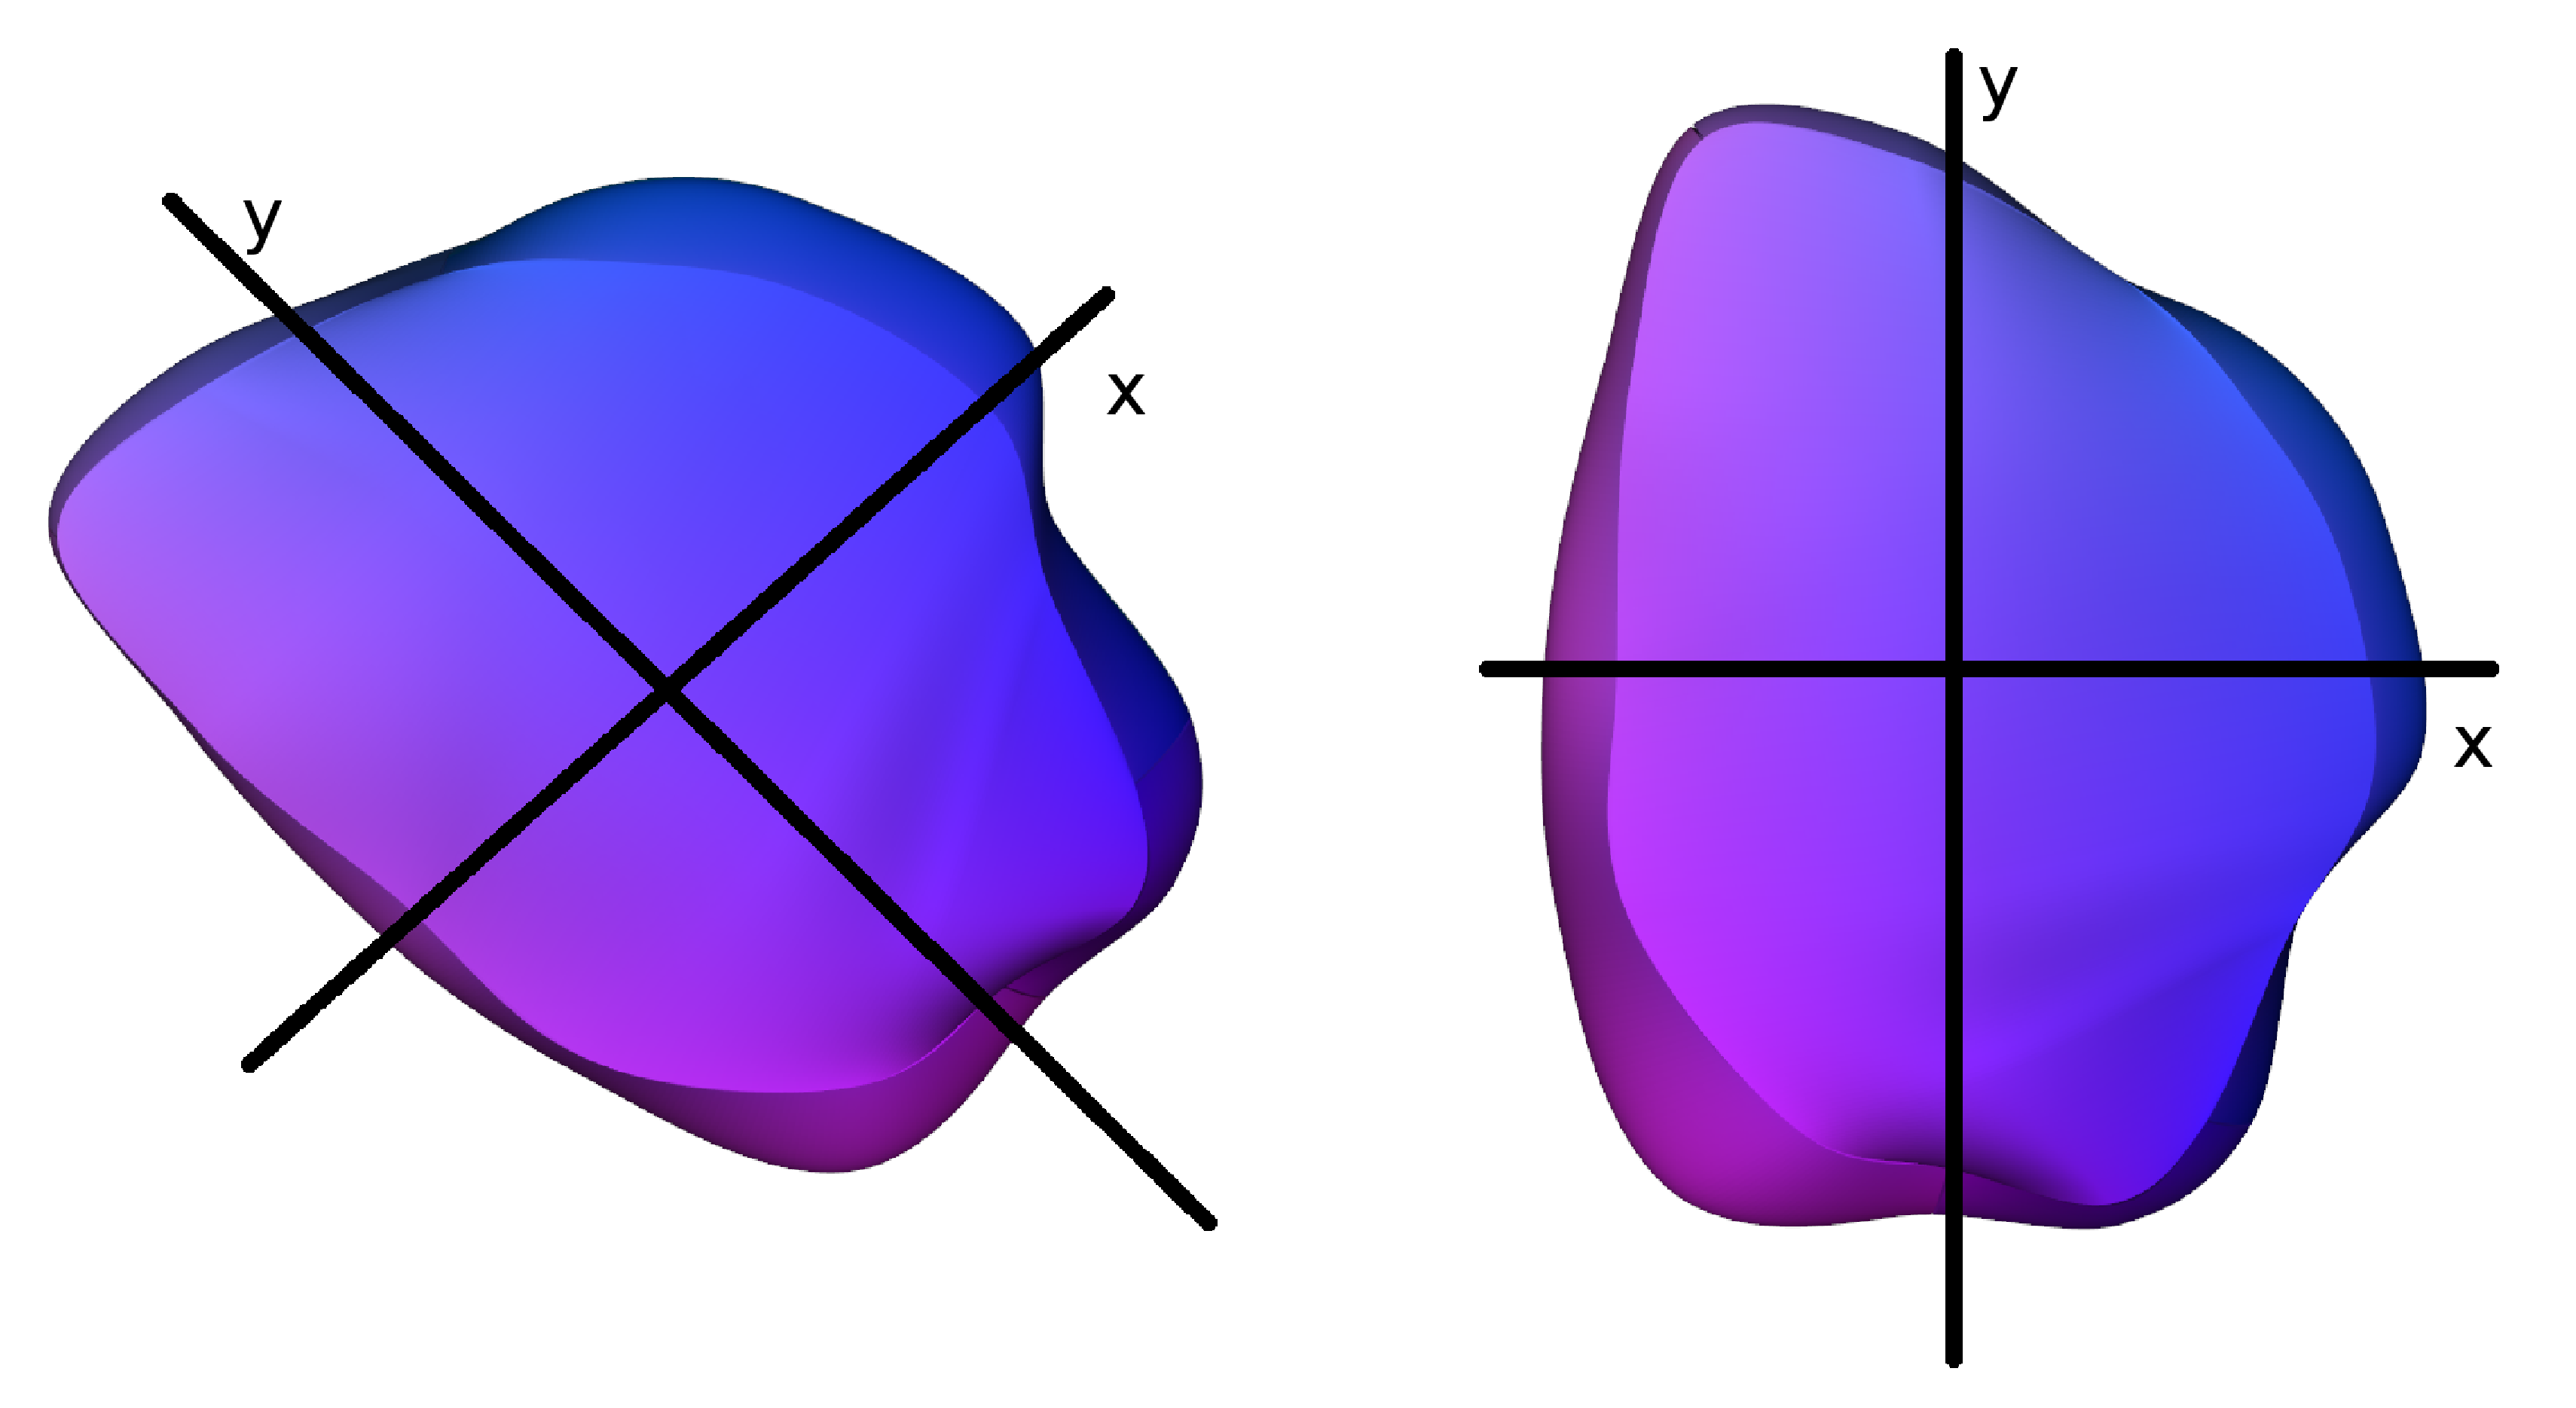
\epsfig{file = rotation.eps, width = 8cm}
 \caption[Rotated figure.]{Figure rotated 45 degrees clockwise.}
 \label{fig:Rotation}  
\end{figure}

Since a rotation can be expressed in matrix form,
the alignment problem can be done 
iteratively by minimizing the distance from the points 
in two objects as shown in Equation \ref{equ:align1}.

\begin{eqnarray}
  [\hat{\Omega}] = \operatorname*{arg\,min}_{\Omega} || \Omega O_i - TO_i||
  \label{equ:align1}
\end{eqnarray}
where $\Omega$ is a rotation matrix around the centroid of the object.
$O$ is an object and $TO$ is a target object or template where both objects are centered on the origin and have unit scale.
The problem consists in finding a matrix $\Omega$ such that the distance from points in $O$ is minimum
to the points in $TO$.

Using matched landmarks 
in a population of objects, this enables the study of shape by 
analyzing the displacements of the landmarks from the target to each object across the population. 

Further improvements of landmark representations sought to produce constrained diffeomorphic deformations i.e., 
differentiable maps that have a differentiable inverse. 
Without the constraint, mapping an unfolded template to a folded structure 
produces non diffeomorphic defformation and
causes to lose the geometry and topology of the template.

\cite{joshi2000landmark} associated the transformation with an energy term,
forcing the existence and uniqueness of the solution, 
thus, enabling the creation of smooth differentiable maps.
This causes the landmarks to deform correctly to the target object and preserve the topology even if 
it is curved. 

Although landmark matching performs well in the study of biological shape and
is able to compute statistics from landmark displacements that 
capture information on scale, translation, rotation and shear.
Information on bending, widening and elongation 
are not very well captured by the approach.
Another major drawback is on landmark positioning.
This is usually done by hand, which is time consuming. 

\subsection{Boundary representations} 

Boundary representation include the following approaches: active contours, active shape/appearance models and projection onto orthogonal functions.

\subsubsection{Active contours} 

Active contours is a method proposed by \cite{kass1988snakes}, commonly known as snakes.
The method was conceived mainly for image segmentation procedures based on curve evolution.

It starts with the definition of a contour $V$ composed by a set of points $p_i$ and an energy function defined for $V$. 
The function has two components corresponding to the internal and external energy in the object being segmented or geometric typicality and
an image match term as defined in Equation \ref{equ:snake}. 

The geometric typicality is responsible for the smoothness of $V$ and its propagation in a desired direction.
Smoothness is controlled by $Econtinuity$ and the direction of propagation by $Eballoon$, ensuring that
the snake curve keeps propagating in the desired direction. 

The image match term takes into consideration the intensity pattern around each vertex $p_i \in V$.
$Eintensity$ makes $V$ move to a region of low or high image intensity information and 
$Egradient$ attracts $V$ to the edges of the object being segmented. 
The whole energy of the contour is defined by the integral in Equation \ref{equ:snakeEnergy}.

\begin{eqnarray} 
 E(V(s)) = \alpha Eint(V(s)) + \beta Eext (V(s)) ds\\
 Eint (V) = \gamma Econtinuity (V) + \delta Eballoon (V)\\
 Eext (V) = \eta Eintensity (V) + \varphi Egradient (V)
 \label{equ:snake}
\end{eqnarray}

\begin{equation}
 E_{snake} = \int_0^1 E(V(s)) ds\\
 \label{equ:snakeEnergy}
\end{equation}

\begin{figure} 
 \centering 
 \epsfig{file = snakes.eps, width = 8cm}
 \caption[Snake's energy.]{Image taken from \cite{kass1988snakes}. The contour moves back to the edge of the pear.}
 \label{fig:snakes}  
\end{figure}

As shown in Figure \ref{fig:snakes}, the contour maps back to the edge of the pear after the perturbation; 
this place is where the minimum is found.

Two major drawbacks of the active contour model are in the initialization step 
since the countour must be placed according to the object being segmented, 
and the need for the boundaries of the object to be defined by a gradient, i.e., to have a smooth boundary with contrast everywhere. 

\cite{chan2001active} proposed an active contour model based on the segmentation 
techniques by \cite{mumford1989optimal} and the level set method. 
The level-set method 
models the internal information of an object.
An example of a level set method is the DT (distance transform).
The DT labels each pixel in the image with the distance value to the nearest boundary point, 
having $0$ at the boundary and either positive or negative in the interior and exterior of the object. 
Even though this information could be 
used to locate and reference the position of internal features in the object, 
the information is only used to 
produce boundary segmentations 
or in other words, to model the curve/surface propagation flow until reaching a stable position.

Figure \ref{fig:chanveseS} shows the automatic segmentation of an object whose boundaries are not well defined and 
the contour can be place anywhere in the image.

\begin{figure} 
 \centering 
 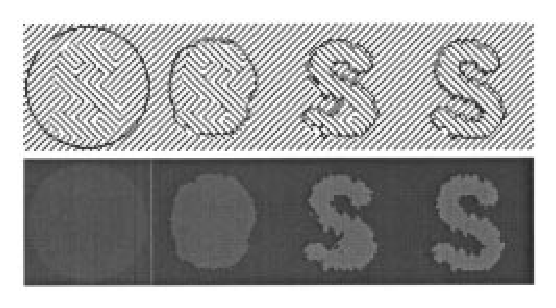
\epsfig{file = chanVeseS.eps, width = 8cm}
 \caption[Segmentation with orientation.]{Image taken from \cite{chan2001active}. The contour of 'S' is not well defined, the segmentation succeeds due to the grouping based on orientation identity.}
 \label{fig:chanveseS}  
\end{figure}

In some situations the regions that are being segmented could be divided, due to high noise on the image or occlusion.
To solve this problem, \cite{jeanvariational} proposed a region growing approach that includes
different type of descriptors in the minimization process.

The approach defines regions in the image via a discrete function:

\begin{equation}
  \phi^{n}(x) =  \begin{cases}
			   1, \text{for $x$ } \in \Omega_{in} \\
			   0, \text{for $x$ } \in \Omega_{out}, 
		 \end{cases} 
   \label{equ:vrgRose}
\end{equation}
where $\Omega_{in}$ and $\Omega_{out}$ are the regions that correspond to the segmented pixels.
The regions defined in $\Omega$, change according to the region-based energy $J(\phi^{n})$, which must
be designed so that its minimum corresponds to the expected solution. At each iteration $n$, the voxels that are connected to $\Omega_{in}$
are tested. If the addition of those voxels decreases the energy, then, they are accepted and the discrete function is updated as

\begin{equation}
 \phi^{n+1}(x) = \frac{1}{2}(1-sign\left(\Delta J(\phi^{n+1})\right).
\end{equation}

This approach has been tested in segmentation of the vascular tree in the lung as shown by \cite{PRIE-12c}, \cite{PRIE-12e}.
The descriptors used on the images are based on a vesselness criterion proposed by \cite{springerlink:10.1007/BFb0029240} and on the gray levels of the original image.
The objective is to detect tubular structures in the image.

The complete formulation using the vesselness descriptors is as follows:
\begin{equation}
  \Delta{J(\phi^{n+1})} = 1 - 2\phi^{n}\left(\Delta{J_{1}}(f, v)\right),
\end{equation}
\begin{equation}
  \Delta{J_{1}}(f, v) = \begin{array}{l}
                         \frac{v}{MaxV} \left( |v - \mu_{v_{in}}|^2 - |v - \mu_{v_{out}}|^2 \right)   \\
			+  \left|\frac{f}{MaxF}\right| \left(|f - \mu_{f_{in}}|^2 - |f - \mu_{f_{out}}|^2 \right),
                        \end{array}
\end{equation}
where $MaxV$ is the maximum value of the vesselness criterion, $\mu_{v_{in}}$ and $\mu_{v_{out}}$ 
are the mean values of the vesselness image voxels in $\Omega_{in}$ and $\Omega_{out}$ respectively. 
$MaxF$ is the maximum value in the original image, and similarly $\mu_{f_{in}}$ and $\mu_{f_{out}}$ are the respective mean values in the image 
for the regions $\Omega_{in}$ and $\Omega_{out}$.

After the segmentation is done by any of the curve evolution methods stated above, 
the user is left with a set of points that correspond to the boundary of the object. 
Once again, notice that the approaches lack the mechanisms to describe internal features of the objects.

The following section introduces segmentation using combined geometric and intensity models, know as active shape and appearance models. 

\subsubsection{Active shape and appearance models} 

ASM (Active shape models) was proposed by \cite{cootes1995active}. 
The approach is based on the formulation that complex images can be analyzed by using 
shape priors. 
It differs from previous approaches that search to segment structures based 
on edges or homogeneous regions by introducing a deformable model template of the
objects that exist in the image. 

A deformable template is defined as proposed by \cite{fisker2000making}:

\begin{definition}
  A \textbf{deformable template} model can be characterized as a model, which under an implicit or explicit optimization
  criterion, deforms a shape to match a known type of object in an image. 
\end{definition}

The segmentation procedure uses the deformable template 
and tries to minimize an energy function that matches the template 
on the image.
In general terms, the approach could be described as observe, learn and match.

The observation stage consists in generating the set of 
training cases. To do this, each object or structure of interest is
represented by a set of points or landmarks. These points can represent
the boundary and internal or external features. 
For each case, the points are required to be 
placed in the same manner. This task 
is usually performed by hand and validated by an expert. 
Although automatic methods have been proposed to speed up the process \cite{hill2000framework}, \cite{heimann2007shape},
the outputs are often revised and corrected. 

Once the landmarks are placed on each training case, they are aligned to a common set of axes.
Recall that if the cases are not aligned, the statistics are meaningless.

After the alignment, the learning stage is done using PCA (principal component analysis); see Appendix \ref{sec:apendixPCA} for details.
PCA detects salient features or principal directions of variation,
removes redundant information and produces a compact representation of the data.

Once the principal direction of variation is detected in the population, 
any of the training sets in the data can be approximated using
\begin{equation}
 x_i \approx Pb + \bar{x}
 \label{equ:approxData}
\end{equation}
where $P = (p_1 |p_2 | . . . |p_n )$ contains $n$ eigenvectors (produced by PCA)
and $b$ is a $n$ dimensional vector that defines a set of 
parameters of a deformable model. 

The variance of the $i_{th}$ parameter of $b_i$ across the training set is given by $\lambda_i$. By applying limits
$\pm 3 \sqrt{\lambda_i}$ the resulting model is guaranteed to be in the population. 

The final stage is to match a new input to the training cases.
This could be done in an iterative process. 
Using the alignment explained in section \ref{sec:surfaceRep},
the matching of a new object $x_i$ goes as follows: 

\begin{enumerate}
 \item Initialize $b$ to zero.
 \item Generate a model $y$ using Equation \ref{equ:approxData} and appearance information.
 \item Align $y$ to $x_i$ using the transformation $\Gamma$ given by Equation \ref{equ:align1}.
 \item Project $x_i$ into model coordinates using $\Gamma^{-1}$, $x_i' = \Gamma^{-1}(x_i)$.
 \item Project $x_i'$ into the tangent plane to $\bar{x}$ by scaling: $x_i'' = x_i'/(x_i' \cdot \bar{x})$
 \item Update $b = P^T (x_i'' - \bar{x})$
 \item Repeat from 2 until convergence.
\end{enumerate}

This general approach to match shape has proven to be very effective in image segmentation. 
It has been applied in applications such as object tracking, detection and recognition.

The AAM (Active Appearance Model) proposed by \cite{cootes2001active} improves the ASM by learning image appearance
statistics as well as the location 
of the landmarks, i.e., each appearance vector is built from the image intensities (grey level or multiple components as RGB).
PCA is applied separately on the landmark information of appearance and location.

A third PCA is applied to search for correlation between the shape and appearance analysis. 
This final PCA is the one used to produce the approximations of a new model.

A speed-up of the method was also proposed by \cite{mitchell20023} where the search for the closest model is done in a multi-scale 
fashion. 

In general terms ASM and AAM are robust and efficient methods in image segmentation, 
we will see in section \ref{sec:medialRepresentations} that 
other methods similar to PCA are best suited to produce statistical information for 3D shape analysis.

\subsubsection{Function based models} 

Function based modeling offers great flexibility and precision. 
The key concept is to use a set of smooth functions to approximately model the surface of an object.
One of the strengths of using such functions is that the derivatives of the object's surface are available and 
boundary normals and curvatures can be derived analytically. 
In contrast to PDM (point distribution models such as landmark based or ASM), these methods efficiently represent
a shape model by using fewer parameters.

Different types of functions can be used to reconstruct a surface, including 
orthogonal functions and spline based methods such as NURBS (Non-Uniform Rational Basis Splines).

There are many type of orthogonal functions: spherical wavelets \cite{schroder1995spherical}, 
SPHARM (spherical harmonics \cite{brechbuhler1995parametrization}, 
Hermite polynomials \cite{bradley1997geometric}, among others.

Spherical Wavelets describe surfaces that have spherical topology.
A wavelet is a function that localizes a given function in space and scale.
In other words, wavelets can represent a given function at multiple levels of detail
and in multiple regions. 
They are superior to a conventional Fourier transform
because they capture 
low and high frequency components of the signal at
specific locations in time or space.
Equation \ref{eqn:wavelet} shows the general formula of a wavelet.

\begin{eqnarray}
 \Psi_{a, b}(t) = \frac{1}{\sqrt{a}}\Psi(\frac{t - b}{a}) \\
 x_a(t) = \iint x(t) \Psi_{a, b}(t)dt
 \label{eqn:wavelet}
\end{eqnarray}

To create a spherical wavelet, the shape of the object is mapped onto the sphere,
and a signal is sampled from it \cite{schroder1995spherical}.
The signal is decomposed in various steps of subsampling and differentiating.
At the end, the procedure retains a coarse representation of the sphere. 
To recover the information lost during the sumbsampling of the signal, a Haar-like operator
is used such that it retains the differences between the two stages \cite{schwartz2008tr}.
The wavelet signal can be used for (lossy) signal compression and can be further analyzed
by PCA. The analysis by PCA yields a mean shape that contains global information 
about the population. 
One of the major drawbacks of the approach lies in the fact that they are only able to represent 
objects of spherical topology. 
A second issue is also found for objects that need to be mapped 
on a sphere to produce the transformation. The mapping can introduce undesired distortion. 


SPHARM functions only represent objects with spherical topology. 
This approach starts by unfolding and mapping the object onto a sphere, where each 
point can be expressed by two parameters in spherical coordinates $(\theta, \phi)$. 
An optimization is performed over the projected points that aims to preserve the area of original
surface elements and minimize their distortion. 
Once the spherical parameterization is obtained, 
the surface $\vec{v}(\theta, \phi) = (x(\theta, \phi), y(\theta, \phi), z(\theta, \phi))^T$
can be expressed as
\begin{equation}
 \vec{v}(\theta, \phi) = \sum_{l=0}^\infty \sum_{m=-l}^l \vec{c}_l^m Y_l^m(\theta, \phi)
 \label{equ:sphericalHarmonics}
\end{equation}
where a least-squares procedure 
finds the best coefficients $\vec{c}_l^m$ for the spherical harmonic basis functions $Y_l^m(\theta, \phi)$, 
for a review on spherical harmonic functions see \cite{mohlenkamp2010user}.
Image \ref{fig:spharm} shows a lateral ventricle surface using different harmonics.

\begin{figure} 
 \centering 
 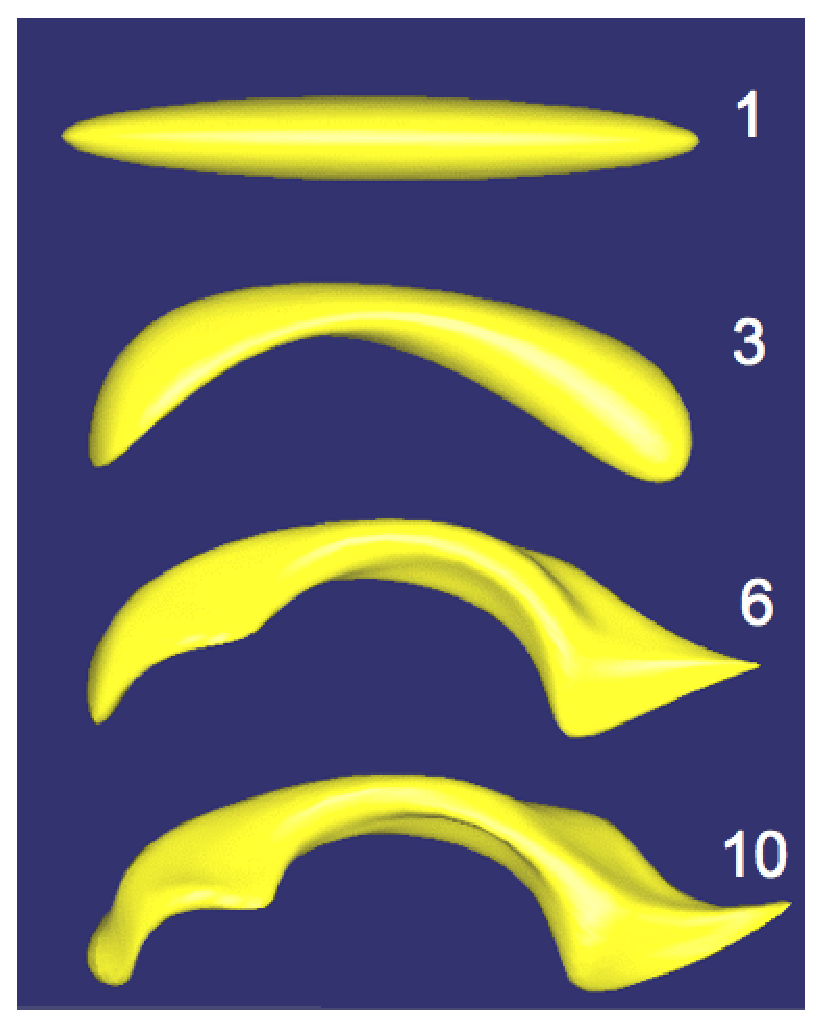
\epsfig{file = spharm.eps, width = 6cm}
 \caption[SPHARM description.]{Image taken from \cite{styner2004boundary}. The SPHARM shape description of a human lateral ventricle 
	  shown at 4 different degrees ( 1, 3, 6, 10 harmonics).
}
 \label{fig:spharm}  
\end{figure}

SPHARM functions were used to estimate the age of a person based on the 
shape analysis of 3D X-ray CT images of human fourth ribs \cite{PRIET-12d}.

Other type of functions can be used to model an object's surface. I am interested in 
the Hermite based functions and spline based methods. They will not be detailed in this section
as they will be reviewed in Section \ref{sec:s-repImplementation}.


\section{Solid representation}
\label{sec:solidRep}

\subsection{Atlas based deformable models}
\label{sec:atlasDeform}

Atlas based deformable models are included in solid representation 
because the geometry of the template (atlas) is well known, 
including its surface and internal features. 

The atlas deformation is based on image registration techniques.
To define image registration, I take the following definition given by \cite{brown1992survey}:

\begin{definition}
 \textbf{Image registration} can be defined as a mapping between two images both
 spatially and with respect to intensity.
\end{definition}

This matching produces deformation maps where every position $p_i$
in the atlas $I_a$ is known on the target $I_t$, therefore 
a registration can be expressed as
\begin{equation}
 I_a(p_i) \approx g(I_t(f(p_i)))
\end{equation}
where $f(p_i)$ is a spatial coordinate transformation
and $g$ is an intensity transformation.

Using the deformation maps, the position of every voxel 
(including internal features) from the atlas can be found on 
the target object. 

To produce the registration, the transformation uses different image descriptors and spatial information. 
The mapping finds an optimal solution, where the optimum depends on the type of descriptors.
For an updated review on image registration techniques see \cite{wyawahare2009image}.

The outputs produced by registration techniques are smooth diffeomorphic maps; 
this means that local structure is also preserved during the deformation \cite{narayanan2005diffeomorphic}. 
For this reason, they have been used to develop transformation-based
probabilistic atlas as shown by \cite{cao2005large} where it describes the variation of ventricular geometry 
and fiber organization (internal features).

Popular software suites for unsupervised segmentation and labeling of structures in the brain
can be found in Freesurfer \cite{fischl2002whole}, \cite{fischl2004automatically} and 
BrainVisa \cite{pohl07_3}. Both are atlas based registration techniques. 

Even though, image registration is known to have to much uncertainty,
it is an approach broadly use for medical image analysis. 
It is difficult to evaluate how well the procedure performs and this is  
a critical point for medical diagnostics, where accuracy is needed. 
Uncertainty arises because the registration produces a single deterministic answer.
Some authors propose solutions to solve this issue by doing posterior statistical analysis 
based on the intensity information \cite{kybic2010bootstrap}, \cite{simonson2011image}.

Measuring uncertainty is helpful to determine whether the results 
can be trusted or not. This measure could possibly be exploited
in unsupervised segmentations or a multi-atlas registration scenario, by giving weights to each atlas based 
on their performance. 
In any case, statistics on deformations are still not adequately developed and remain the major
drawback of the approach. 

The following section is for medial representations, the type of modeling that will be used throughout
this dissertation. 

\subsection{Medial representations}
\label{sec:medialRepresentations}

\begin{chapquote}{Harry Blum}
  For even so simple a notion as location of an object, the contour or perimeter description is particularly poor.
\end{chapquote}

The concept of medial representation started with \cite{blum1967transformation}.
Blum noticed that for any shape, it was possible to calculate a medial axis and 
by doing it, the objects can be described from the inside, in contrast to the techniques 
in Section \ref{sec:surfaceRep}, that seek to model the outside of the object only.

To explain this concept Blum used a grassfire analogy, where the formation of the medial axis is done by setting fire to 
the outer layer of the object i.e., its boundary. The fire propagates uniformly towards the interior of the object and 
when the fronts meet we find the medial axis, a notion related to level-set. 
Following this concept the definition of a medial axis is as follow:

\begin{definition}
 The \textbf{medial axis} is the collection of interior points with at least two closest points on the boundary.
 \label{def:medialAxis}
\end{definition}

In conjunction with the MA (MA will be use to denote medial axis or medial locus similarly) a MAT (medial axis transform) is generated: 

\begin{definition}
 The \textbf{medial axis transform} contains the distance from each point of the medial axis to the boundary of the object. 
\end{definition}

In the context of the grassfire analogy, the MAT adds to each axis point a value equivalent to the burning time from the boundary 
until two fronts meet at the MA.
The MAT has been criticized as small boundary perturbations produce significant changes
on the MA, which yields it impractical for shape description. Figure \ref{fig:unstable} shows 
an example of unstable MA.
This instability has been the focus of many research groups that seek 
to produce a better computation of the MA. 
The idea is to identify the most meaningful 
subsets that compose the MA by trading exactness for stability.

Typically, a pruning of the MA is performed by a threshold value and a criterion that determines
``substance'' and ``connection'', substance being the tangible part of the object and connection, 
how the parts are connected. 
To have a better understanding of this concept think of a complex object such as a hand. 
A hand is compose by a palm (a blob) and fingers (protrusions) or 
think of it as a collection of more complex objects. The substance is
connected in a such a way that we perceive a hand.

\begin{figure} 
 \centering 
 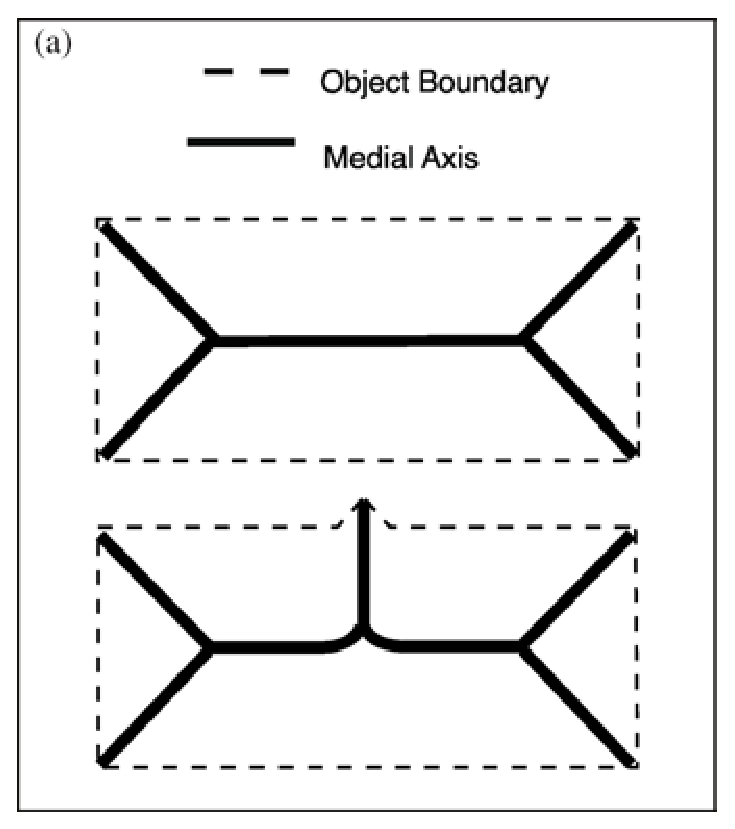
\epsfig{file = medialUnstability.eps, width = 8cm}
 \caption[MAT instabilities.]{Image taken from \cite{katz2003untangling}. MAT instabilities: A tiny change in the boundary produces a large change in the MAT.}
 \label{fig:unstable}  
\end{figure}

Different authors provide the means of computing stable MA: see the methods by
\cite{culver1999accurate}, \cite{amenta2001power}, \cite{katz2003untangling}, \cite{miklos2010discrete}. 

A stable MA is a powerful shape descriptor that
produces compact shape representations of the surface of an object and provides better notions of concepts such as ``center point'' and 
positions inside and relative to the object.
As mentioned in section \ref{sec:surfaceRep} the centroid is used
to align objects on a common frame. In some cases the centroid 
of an object is outside the object itself, thus, making it unsuitable for alignment procedures.
By computing the center point on the MA, it is guaranteed that it will 
be inside the object and its position will be stable under different transformations of the object \cite{liu2011extended}.

The notions such as a position inside the object or relative to other objects are not addressed 
by any of the techniques discussed in Section \ref{sec:surfaceRep}.
These are trivial when an object is described by its MA. 
Positions inside the object will be discussed later in Section \ref{sec:internalCoordinates}.

In 2D the MA is created by computing maximally inscribed discs, with at least two 
points on the boundary. The union of disk's centers form the MA.
In 3D the MA is composed by sheets, generated with maximally inscribed spheres.
In general terms, the MA extends in higher dimensions, where it is composed by hypersurfaces
generated with maximally inscribed hyperspheres.

\begin{figure} 
 \centering 
 \subfigure[Growing]{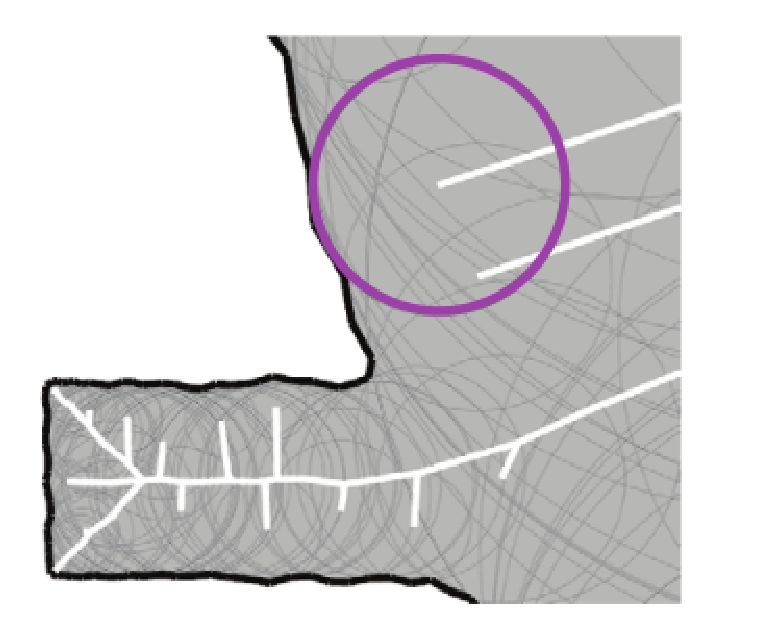
\epsfig{file = StableMedialAxis0.eps, width = 4.5cm}}
 \subfigure[Shrinking]{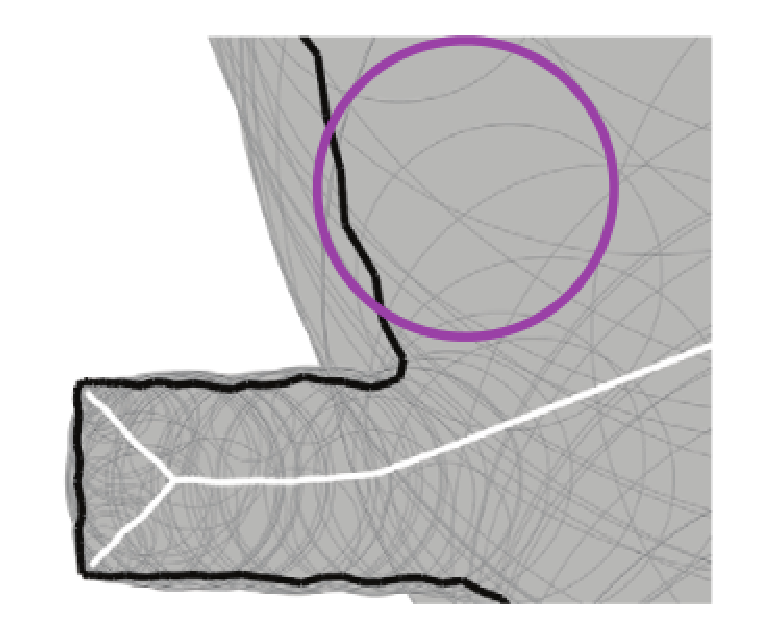
\epsfig{file = StableMedialAxis1.eps, width = 4.5cm}}
 \subfigure[Pruned]{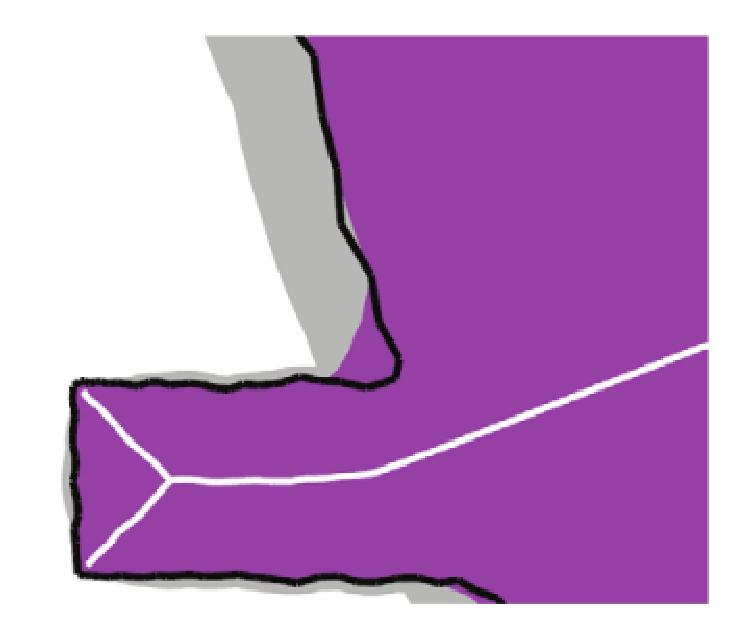
\epsfig{file = StableMedialAxis2.eps, width = 4.5cm}}
 \caption[MA Pruning.]{Image taken from \cite{miklos2010discrete}. Pruning the medial axis to detect important features.}
 \label{fig:stableAxis}  
\end{figure}

To get an insight of one technique to compute a stable MA, let us take the example in 
figure \ref{fig:stableAxis}. Figure \ref{fig:stableAxis}.a shows 
the MA in white and a medial inscribed disk in purple.
Figure \ref{fig:stableAxis}.b shows the same disc scaled by $\delta$. 
When all discs are scaled, large discs cover smaller nearby
discs. Covered discs belong to branches that can be trimed. 

Using this criterion, the branches can be pruned using a
scaling factor $\delta$, keeping only the larger discs 
that belong to the 'substance' of the object.

Figure \ref{fig:stableAxis}.c shows the simplified MA after
the shrinking of the discs by the same $\delta$. 
This procedure detects the least important branches on the MA, and
by pruning them, the amount of data to represent the same figure with out loosing 
much precision is significantly reduced. 

One important aspect left unanswered is if this type of representation 
is adequate to perform statistical analysis on a population of objects. 
One major difficulty will be to produce the correspondence of the branching structures.
Statistics on branching objects is a subject of ongoing research by \cite{wang2007object}, \cite{sorensen2011dissimilarity}, 
\cite{aydin2011visualizing}, 
which is still not applicable to medial geometry. 
To use medial representations for statistical analysis on shape, 
the construction of the MA must be done in a different manner: 
the MA should have a stable structure for the population of objects we wish to represent. 

If we take into consideration how the MA is built, we see that the procedure is a top-down approach, 
it starts on the boundary of the object and by using a certain criteria it gets to the MA. 
Another alternative is to operate the opposite way (down-top). 
We can find a down-top approach to build a MA in \cite{styner2001medial}.

In summary, Styner's method goes by computing an average MA
from a population of objects and then sampling the average using a regular grid of
points. The sampled grid of points is used as the new MA.
To compute the average MA, a PDM of
the branching structures is created 
by finely sampling their SPHARM representations.
The PDM allows PCA to compute the average and 
finally the grid of points or m-rep (definition given shortly) is sampled by 
minimizing a distance function over the points.
A series of tests are performed afterwards to assess
the quality of the MA by 
generating different instances of the population using 
the PCA coefficients. For each instance, the m-rep is refitted,
and an error measurement is estimated to evaluate 
how well it represents the whole population. 

\begin{figure} 
 \centering  
 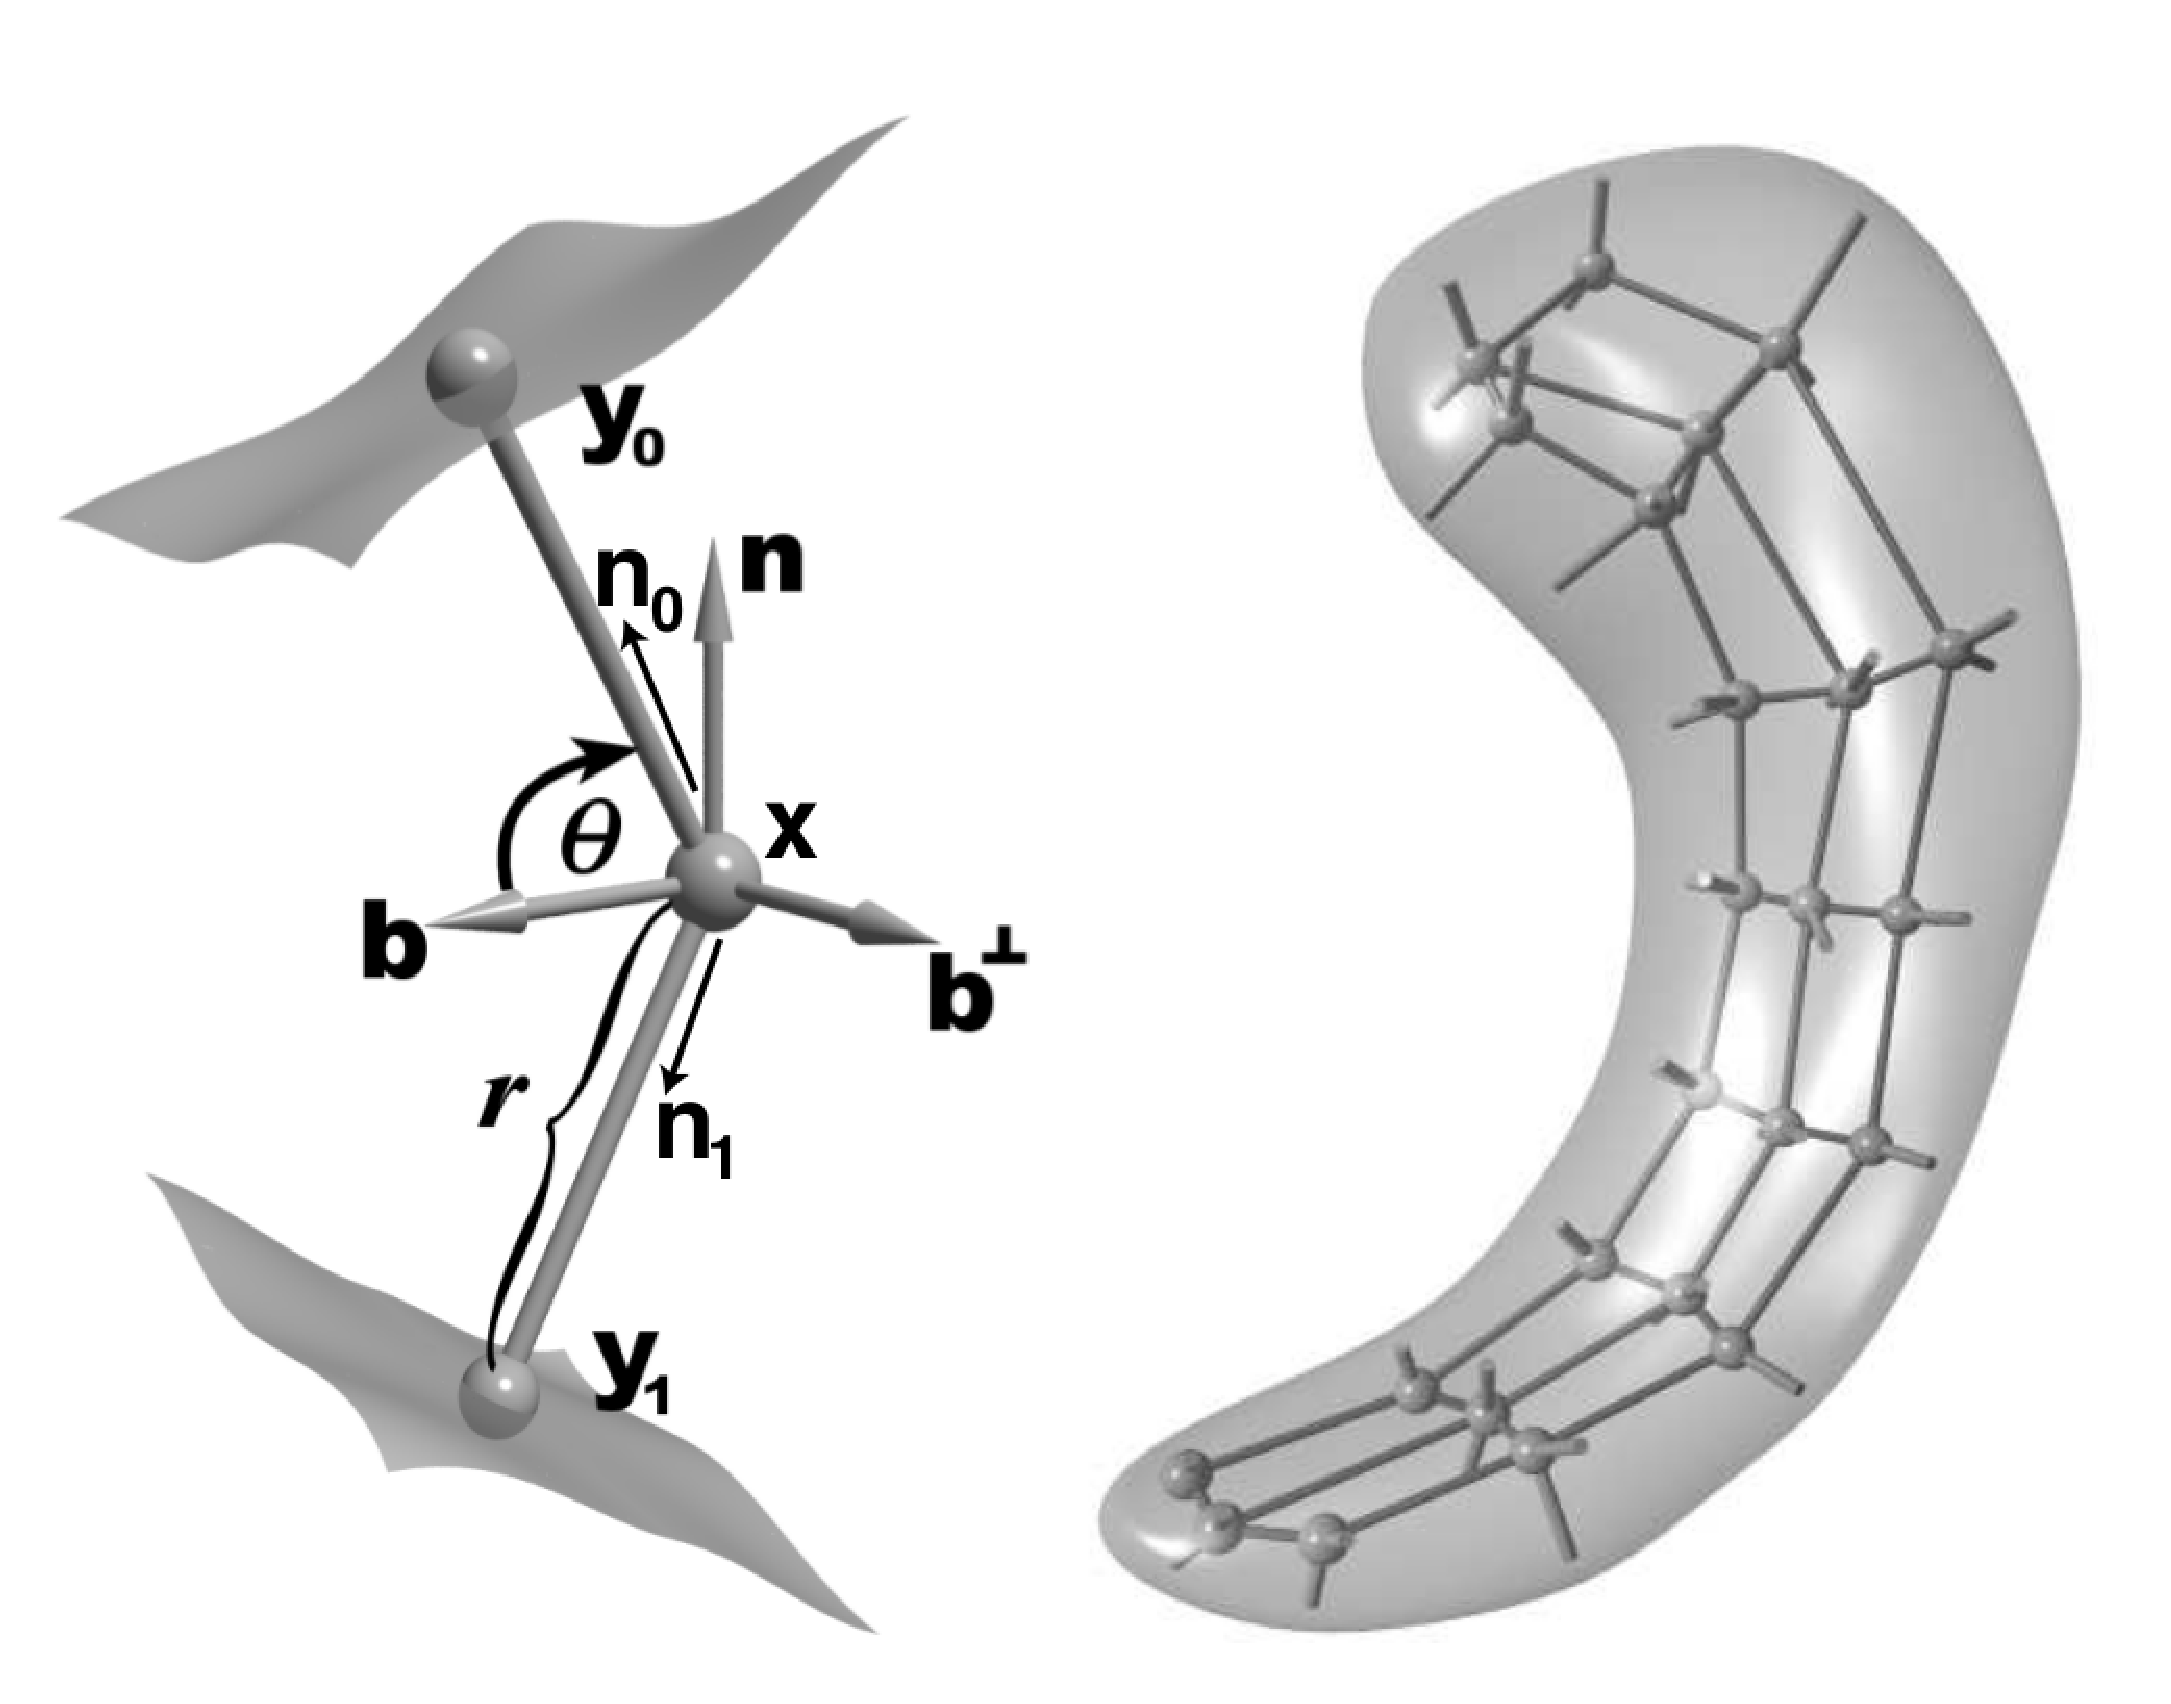
\epsfig{file = medialGeometry.eps, width = 8cm}
 \caption[Medial atom definition.]{Image taken from \cite{fletcher2004principal}. Medial atom definition (left) and a set of atoms representing a hippocampus (right).
          The atoms are arranged in a grid size $8*3$ and are able to produce the boundary of the hippocampus.}
 \label{fig:3DmedialGeometry}  
\end{figure}

M-reps are continuous objects that define the MA of an object as 
a set of connected manifolds \cite{pizer1999segmentation},  \cite{yushkevich2003continuous}, \cite{pizer2003deformable}.
Figure \ref{fig:3DmedialGeometry} shows the components of the medial geometry. 
The MS (medial sheet, equivalent to MA in 2D)
is parameterized by $MS(u, v)$ where $u$ and $v$ can take any value between 
$[0, 1] \in R$. 
The MS is a $C^2$ continuous set of medial atoms with a corresponding
implied boundary $y_{0}$ for top surface and $y_{1}$ for bottom surface. 

\begin{equation}
 MS(u, v) = \{x, r, n_0, n_1\}
 \label{equ:medialSheetAtom}
\end{equation}
Equation \ref{equ:medialSheetAtom} defines an atom for 
every $(u, v)$ on the MS, 
where $x$ is the position on the MS, $n_0$ and $n_1$
are the unit spoke directions, and $r$ is the 
length of both vectors. 

A different type of atom is found at the edges of the figure, named crest atoms.
Figure \ref{fig:crestAtom} shows how the top and bottom surfaces join 
at the crest to produce the closed boundary of the object. 

\begin{figure} 
 \centering  
 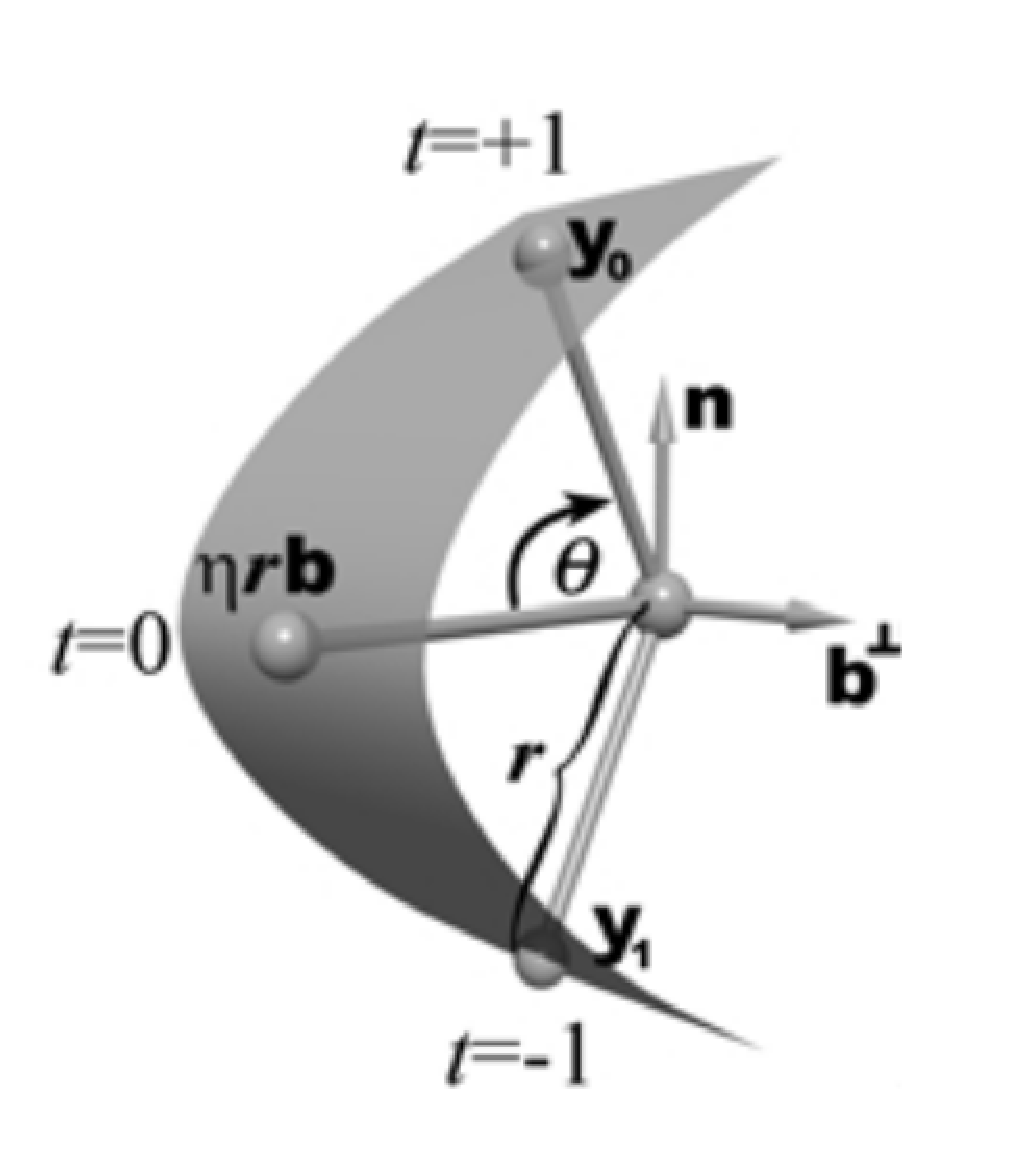
\epsfig{file = crestAtom.eps, width = 8cm}
 \caption[Top, bottom and crest surfaces.]{Image taken from \cite{pizer2003deformable}. Top and bottom surfaces of the m-rep join at the crest.}
 \label{fig:crestAtom}  
\end{figure}

To describe an m-rep in the computer, 
a discrete set of atoms is used.
From now on, the word m-rep relates to the discrete version of the object. 
M-reps use the interpolation mechanisms described in \cite{thall2004deformable}, 
which enables to reconstruct the object's surface.
The interpolation matches the surface 
to the normals described by the vectors $n_0$ and $n_1$.
Matching the normals produces a $C^2$ continuous surface everywhere. 
%From this surface Thall’s method allows the calculation of the interpolated medial atoms.

In summary, m-reps are efficient structures 
that describe in a multi-scale fashion the geometry
of an object, they can be used 
for medical image segmentation \cite{pizer2005method} and perform 
statistical analysis on shape variability \cite{fletcher2004principal}. 

The method used by m-reps to produce statistics is called PGA (principal geodesic analysis)
a generalization of PCA to manifold data, which will be described briefly in the 
following section.

\subsubsection{Principal geodesic analysis}

We have seen that m-reps can represent a population of 3D figures
by defining a stable MS and deforming it to best fit 
the various instances of the objects.
One of the many strengths of m-reps is to describe 
shape changes in terms of thickness, bending and widening 
among the already known variations (translation, rotation and scale).
In order to describe these variations 
standard techniques to compute statistics such as PCA do not apply, 
since m-reps are composed by elements of a non-Euclidean space.
In fact they belong to a Riemannian symmetric space.

If we recall the definition of a medial atom \ref{equ:medialSheetAtom},
we see that it is composed by $x \in R^3$, the center of the
inscribed sphere; $r \in R^+$, the local width defined as the
common spoke length; $n_0, n_1 \in S^2$, the two unit spoke
directions (here $S^2$ is the unit sphere in $R^3$).
The medial atom is then a point on the manifold
$M(1) = R^3 \times R^+ \times S^2 \times S^2$. 
Since an m-rep consists of $n$ medial atoms, 
a single figure may be considered as a point
on the manifold $M(n) = \Pi_{i=1}^n M(1)$ i.e., the direct product
of n copies of $M(1)$.

PGA (principal geodesic analysis) was developed as a generalization of PCA
for manifold data. 
The idea is to project the data onto lower-dimensional 
subspaces that best represent the variability of the data. 
Concepts from PCA such as mean, variance, subspace and projection 
had to be revisited in order to work properly with manifold data.
Details of PGA can be found in \cite{fletcher2004principal}.

PGA works well for data living on manifolds with spherical components, 
especially when the data is concentrated on a great circle path 
since the procedure fits the best great circle to describe these variations.
However, m-rep data frequently lives on small circles
as the mean computed with PGA is not optimal.
A more suitable statistical framework can be developed taking this into consideration. 

The following section describes quasi-medial representations or s-reps and
the statistical framework to compute shape variations called CPNS (composite 
principal nested spheres).


\subsection{Quasi-medial representations}
\label{sec:quasiMedial}

Quasi-medial representations or s-reps \cite{pizer_nested_2012} differ from m-reps on the strict medialness
constraint on every atom, i.e., the position of an atom is not necessarily the center 
of a maximally inscribed sphere. 
In s-reps, the atoms are rewarded for being ``as medial as possible'' but small 
deviations are tolerated, this means that the spokes can have different lengths;
this is done to improve the fit of an s-rep to a given object.

S-reps are continuous objects, defined as a locus of spoke vectors $(p, S)$ 
with tail at $p$ and tip at $p + S$, also parameterized by $(u, v)$ such that 
the skeletal sheet is defined as $SS = \{p(u, v) : \forall (u, v) \in [0, 1] \}$, the
spokes $SP = \{S(u, v) : \forall (u, v) \in [0, 1] \}$ and 
the boundary of the object is $BO = \{p(u, v) + S(u, v) : \forall (u, v) \in [0, 1] \}$.
The union of tails form the skeletal locus as a fully folded 
multi-sided sheet, i.e., the top side of the sheet is parameterized by $v \in [0, 0.5]$
and the bottom side by $v \in [0.5, 1]$.
Given this definition, every point inside the object can be reached by at least one spoke; 
special care in the corners of the object since they are reached by multiple spokes but allow the SS 
to fold and create the interior filling representation.

The lengths of the spokes are defined as $r(u, v) = |S(u, v)|$ and 
the directions of the spokes as $U(u, v) = S(u, v)/r(u, v)$. 
Figure \ref{fig:srepFigure}-a shows a slab figure parameterized
by $(u, v, \tau)$. $\tau \in [0, 1]$ is the portion of the spoke length from the SS to the boundary of the object.
The s-rep description can be used on tubular objects also. 
The tube figure is parameterized by $(u, \phi, \tau)$. Figure \ref{fig:srepFigure}-b shows the 
interior filling representation of a tubular object.

Section \ref{sec:internalCoordinates} extends the concept of interior filling objects and
the generation of $X2U$ (world coordinates to s-rep coordinates) and $U2X$ (s-rep coordinates to world coordinates) maps. 

\begin{figure} 
 \centering  
 \subfigure[Slab]{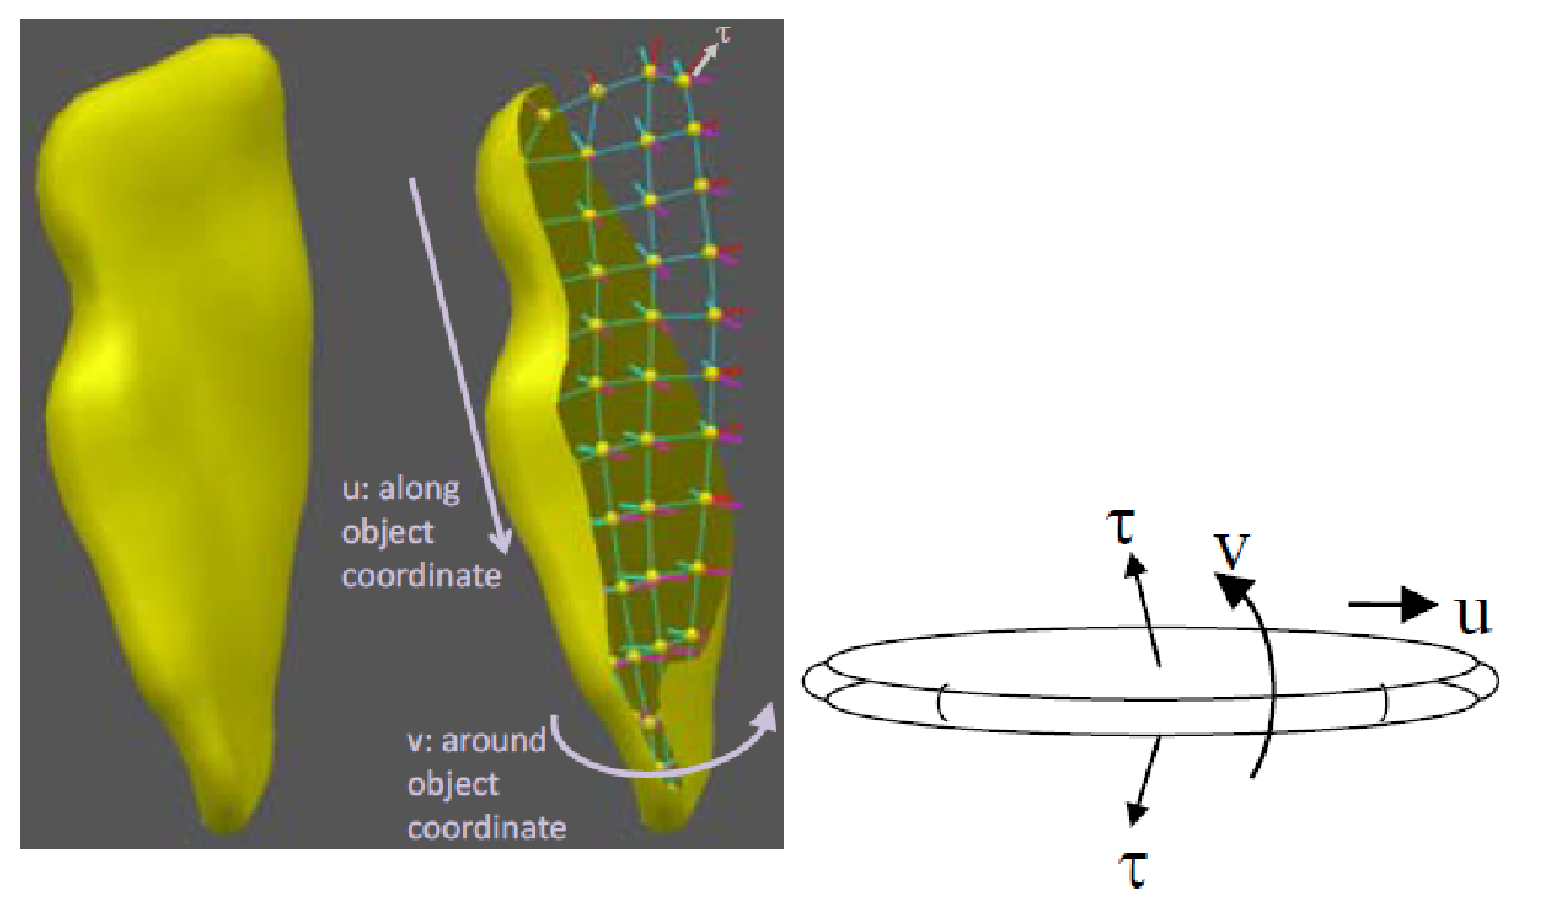
\epsfig{file = s-repSlab.eps, width = 16cm}}
 \subfigure[Quasi-tube]{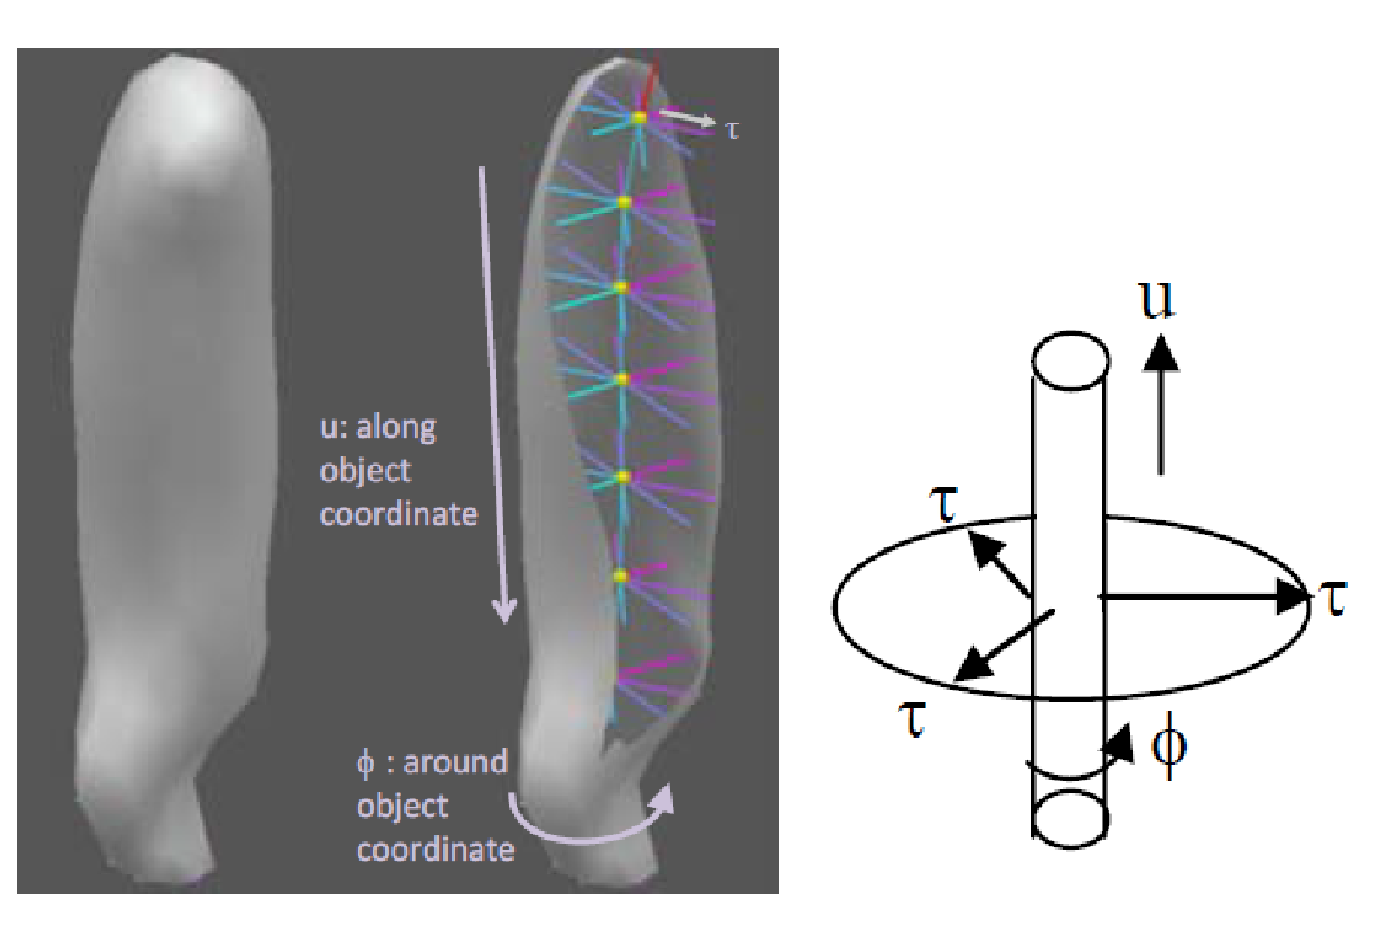
\epsfig{file = s-repTube.eps, width = 16cm}}
 \caption[Slab type s-rep.]{Image taken from \cite{pizer_nested_2012}. S-rep slab, interior filling object. Parameterized by $(u, v, \tau) \in [0, 1]$
          every point inside the object can be reached by only one spoke. 
          Similarly a tube figure is parameterized by $(u, \phi, \tau)$, $\phi$ is the rotation around the space curve that defines the MA.}
 \label{fig:srepFigure}  
\end{figure}

In a similar manner to m-reps, in the computer, s-reps are represented with a discrete set of atoms. 
From now on, s-rep is the discrete version of the object. 
S-reps use the interpolation mechanisms described in \cite{damon2003smoothness},
\cite{han2006interpolation}, \cite{damon2008swept} to produce a smooth skeletal locus and a smooth vector field of spokes that generates the 
boundary of the object.
For slab figures, represented as a $m \times n$ grid of atoms, 
the interpolation defines operators called $S_{rad}(u, v)$ and $S_E(u, v)$, 
applicable to non-fold medial points (top and bottom side of the sheet without the edges) and to the edge of the figure respectively.
The operators are defined as $2 \times 2$ matrices that can be computed for each spoke. They describe how the vector
$U(u, v)$ moves along and across the field of spokes. To interpolate a spoke at position $(u + \Delta u, v + \Delta v)$ 
the method uses the eigen-decomposition of the matrices. Damon shows that the object remains legal i.e., the spokes
do not cross each other,
if and only if for all $(u, v)$ the eigenvalues of $S_{rad}(u, v) < 1/r(u,v)$. 

The field of spokes can be retrieved by taking a small $\Delta$ step in the $(u, v)$ direction and interpolating  
the eigenvalues found from the eigen-decomposition of the matrix. 
The interpolation is done using the neighboring discrete spokes in the quad.

A quad is defined as
\begin{equation}
 Q_{i,j} = \{S(\frac{i}{n}, \frac{j}{m}), S(\frac{i+1}{n}, \frac{j}{m}), S(\frac{i+1}{n}, \frac{j+1}{m}), S(\frac{i}{n}, \frac{j+1}{m}) : i \in [1, n-1], j \in [1, m-1] \}]
 \label{equ:Quad}
\end{equation}
  
At each $(u + \Delta u, v + \Delta v)$ new eigenvalues 
are calculated that can be turned back into an $S_{rad}$ operator. Integrating $S_{rad}$
from $(u, v)$ at the corner to $(u + \Delta u, v + \Delta v)$ following a straight line, 
the full swing of the spoke can be computed. 

Besides object modeling using the interpolation mechanisms just described, 
the goal is to produce s-reps suitable for probabilistic analysis. 
Similarly to m-reps, the MS on an s-rep figure must remain 
stable through the population of objects.
S-reps go through a fitting process to produce the best possible
representation for each subject in the population. 
The procedure has mainly 3 stages to produce the fit. 
First, the s-rep is aligned to the image;
second, each atom is moved around separately to improve the fit; 
third, the spoke lengths are modified to further match the object's
boundary.
Further details are given in the following section.

\subsubsection{S-rep fitting}

The fitting process is done to produce the best 
geometric approximation of an object using 
a base s-rep, thus, stabilizing 
the MS through the population and giving the possibility to 
compute better statistics afterwards.
For the case of s-reps, instead of GPA, CPNS (Composite Principal Nested Spheres) is used.

The s-rep fitting is done on already segmented data, usually provided 
in the form of a binary image. The image is converted into 
a signed distance transform \cite{saboo2011aa}, with negative values 
in the interior, 0 at the boundary and positive outside of the object. 
After the conversion, 
the fitting starts by aligning the s-rep to the data
via matching of moments of boundary positions (zero level on the distance transform) or using 
landmarks provided by the user.

In the second stage or atom stage, each atom in the s-rep is optimized
by measuring how well each of the spokes fits into the distance image $D(x)$ while maintaining 
the regularity of the grid. In this stage, the only variable affected is the position and orientation of the atom. 

In the third stage or spoke stage, each spoke is optimized to produce the best match to the boundary of the object
while fixing the tail and changing the angle and length of the spokes.

The following penalties are used to produce the fit:
\begin{enumerate}
 \item Regularity of the quads (see Equation \ref{equ:Quad} for quad definition). 
 \item Deviation from medialness using the spokes located at opposite sides of the MS $|r(u, v) - r(u, 1 - v)|$. 
 \item Deviation of spoke directions from boundary normals $cos^{-1}(\hat{\nabla D(x)} \cdot U(u, v))$ where $x = p(u,v) + S(u, v)$.
 %\item Deviation from MS normals. The MS normal is calculated as $U(u,v) - U(u,1 - v)$.
 \item Deviation at the crest from the angle between $w_2$ and $U(u, v) \times U(u, 1 - v)$, where $w_2$ is orthogonal to the principal curvature direction.
 \item Illegality of spoke crossings, i.e.,  $S_{rad}(u, v) > 1/r(u,v)$ 
\end{enumerate}

Once the optimization described above is done for every object in the population, 
correspondence among the cases must be achieved prior to computing 
statistics using CPNS; this can be done by using the SS that is composed by 
a set of points $\{p_i\}$ as a PDM. The PDM can be centered at the origin and 
then scaled by making the 
sum of the squared distances of the points to the origin equal to 1.
The scaling factor of the PDM will be named $\lambda$.
After the alignment, in order to produce shape statistics, let us analyze the 
abstract space where an s-rep lives.

\subsubsection{S-rep abstract space and composite analysis}

An s-rep lives in $R^{n+1} \times S^{3n - 4} \times (S^2)^n$.
To explain this abstract space, let us
define one s-rep composed by $n$ spokes $s_{rep} = \{(p_i, r_i, U_i) | i = 1,2, ...,n\}$.
This corresponds to the Cartesian product of $n + 2$ manifolds, 
one of which is Euclidean and the rest are spheres.
The Euclidean manifold $R^{n+1}$ corresponds to $n$ log $r_i$ values plus 
the scaling factor of the PDM (log $\lambda$).
The spherical manifolds are the $S^{3n - 4}$ corresponding to the PDM
and the $(S^2)^n$ are for the $n$ spoke directions.

In order to study a population of s-reps and knowing that 
they are composed by elements on different manifolds, 
each one of them is analyzed separately at first.

PNS (principal nested spheres) \cite{jung_analysis_2012} allows 
estimating the principal modes for each non-Euclidean component
and produces Euclidean scores (see Appendix \ref{sec:apendixCPNS}).
All of the scores are composed on a matrix 
that contains Euclidean data only, thus, 
making possible to do further analysis using PCA. 
The composite matrix $Z_{comp}$ is shown in Equation \ref{equ:compositeMatrix}, where $N$ is the number
of s-reps and * means that the mean has been subtracted from the variable. 

\begin{equation}
\begin{array}{ccc}
         \begin{array}{c}         
          \text{Sphere 0:} \\
          \text{Scaled medial points} \\
           \\
           \\
          \text{Spheres 1 - n:}\\          
          \text{Spoke directions} \\
          \\
          \text{Euclidean variables:}\\
          \text{Scaling}\\
          \\
          \\
          \text{Spoke lengths} \\          
          \\
         \end{array} 
 &
    \left [ \begin{array}{ccc}
          z^t_{1,1} & \hdots & z^t_{1,N} \\
          \vdots    & \ddots & \vdots    \\
          z^t_{N-1,1} & \hdots & z^t_{N-1,N}\\
          \\
          z^{S_1}_{1,1} & \hdots & z^{S_1}_{1,N}\\          
          \vdots    & \ddots & \vdots    \\
          z^{S_n}_{n,1} & \hdots & z^{S_n}_{n,N}\\          
          \\
          \text{log}^*_{\lambda_1} & \hdots & \text{log}^*_{\lambda_N} \\
          \\
          \text{log}^*_{r_{1,1}} & \hdots & \text{log}^*_{r_{n,N}} \\
          \vdots    & \ddots & \vdots    \\
          \text{log}^*_{r_{n,1}} & \hdots & \text{log}^*_{r_{n,N}} \\
         \end{array} \right ]
 &
    \left [ \begin{array}{c}
          \bar \lambda \\          
          \vdots \\
          \bar \lambda \\
          \\
          \bar r_1 \\          
          \vdots \\          
          \bar r_n \\
          \\
          \bar \lambda \\
          \\
          \bar r_1 \\
          \vdots \\
          \bar r_n \\
         \end{array} \right ]
\\
& \longleftarrow \text{Cases} \longrightarrow & \text{Scaling}
\end{array}
\label{equ:compositeMatrix}
\end{equation}

CPNS produces a set of eigenmodes that can be used to approximate 
any of the shapes in the population (see Appendix \ref{sec:apendixPCA}).
This results in a vector that lives in Euclidean space equivalent to the $Z_{comp}$ matrix.
Using this vector, each of the Euclidean components are ready to be mapped back to 
their corresponding spheres by adding the mean value computed at the PNS analysis. 

We have seen that it is possible to compute robust statistics for 3D shape objects using 
medial representations. The following section explains the implementation based 
on the concepts seen for medial representations. 

\section{Object modeling using s-reps }
\label{sec:s-repImplementation}

The s-rep implementation done for this dissertation defines
the interpolation mechanisms similar to \cite{han2006interpolation}.

\subsection{MS interpolation}

The interpolation is done with cubic Hermite splines.
To produce the interpolation, the partial derivatives for every atom on the SS, 
and the normal must be defined.

Let $s_{rep} = \{(p_i, S_i) : i \in N\}$ and $N = m \times n$, 
represent a discrete grid of atoms.
The interpolation is done using the four control points from each quad in the grid. 

%A quad is defined as 
%$Q_{i,j} = \{S(i/n, j/m), S((i+1)/n, j/m), S((i+1)/n, (j+1)/n), S(i/n, (j+1)/m) : i \in [1, n], j \in [1, m] \}]$)),
Equations \ref{equ:pDerivativeU} and \ref{equ:pDerivativeV} shows how to compute the partial derivative for a given atom 
in the $u$ and $v$ direction on the SS. $\Delta u = 1/m$ and $\Delta v = 1/n$ 
correspond to a step lenght. $u + \Delta u$ moves along the $u$ direction onto 
the next atom on the discrete grid, and similarly for the $v$ direction.

\begin{equation}
 \partial p(u, v)_u = \left \{ \begin{array}{ll}
                      p(u + \Delta u, v) - p(u , v) & u = 0\\
                      \big (p(u + \Delta u, v) - p(u - \Delta u, v)\big )/2 & 0 < u < 1 \\
                      p(u, v) - p(u - \Delta u, v) & u = 1
                     \end{array} \right .
\label{equ:pDerivativeU}
\end{equation}

\begin{equation}
 \partial p(u, v)_v = \left \{ \begin{array}{ll}
                      p(u, v + \Delta v) - p(u, v) & v = 0\\
                      \big (p(u, v + \Delta v) - p(u, v - \Delta v) \big ) /2 & 0 < v < 1 \\
                      p(u, v) - p(u, v - \Delta v) & v = 1
                     \end{array} \right .
\label{equ:pDerivativeV}
\end{equation}

Equation \ref{equ:sheetNormal} gives an approximation to the normal of an atom to the SS. 
The normal is computed from opposite spokes with tail at equal position on the SS. 
More precisely, $N$ is normal to the SS if the two spokes are exactly boundary normals 
and have the same lenght. 

\begin{equation}
  \begin{array}{cc}
   N(u, v) \approx \frac{S(u, v) - S(u, 1 - v)}{||S(u, v) - S(u, 1 - v)||}  & u  \in [0, 1], v \in [0, 0.5] \\
  \end{array}
\label{equ:sheetNormal}
\end{equation}

\begin{figure} 
 \centering  
 \subfigure[Level 0]{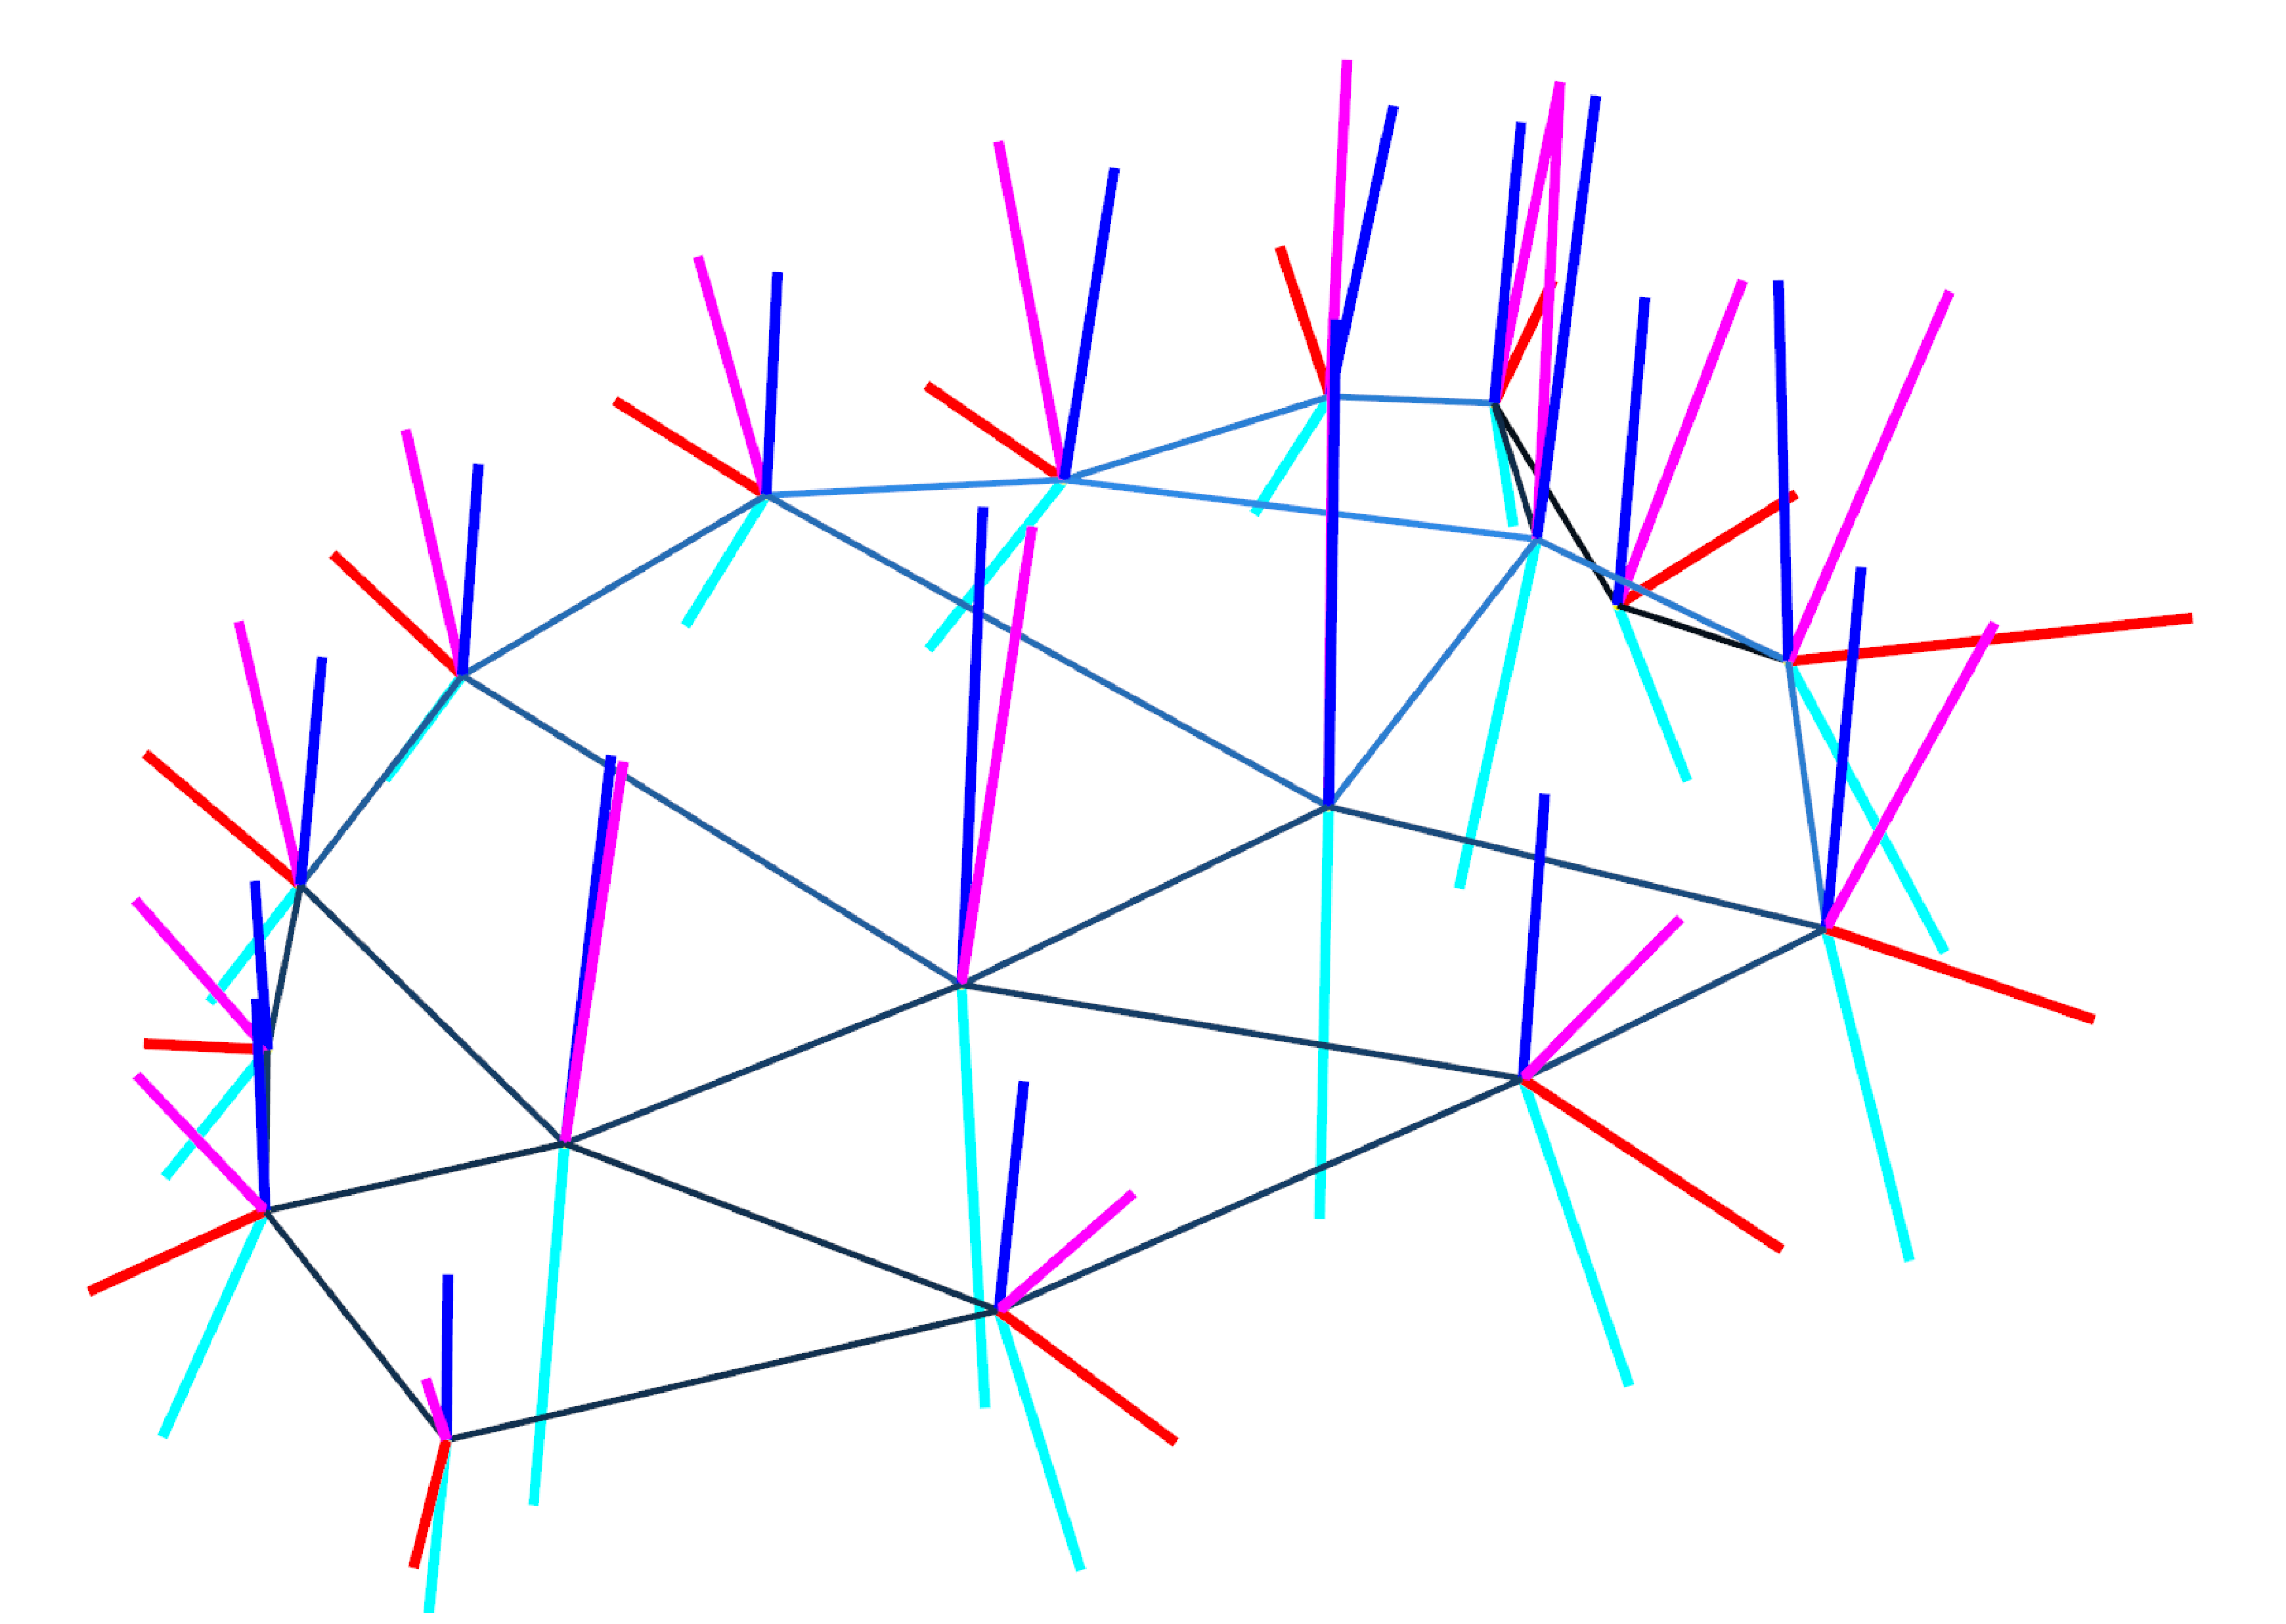
\epsfig{file = interpolationMedialSheet0.eps, width = 7cm}}
 \subfigure[Level 3]{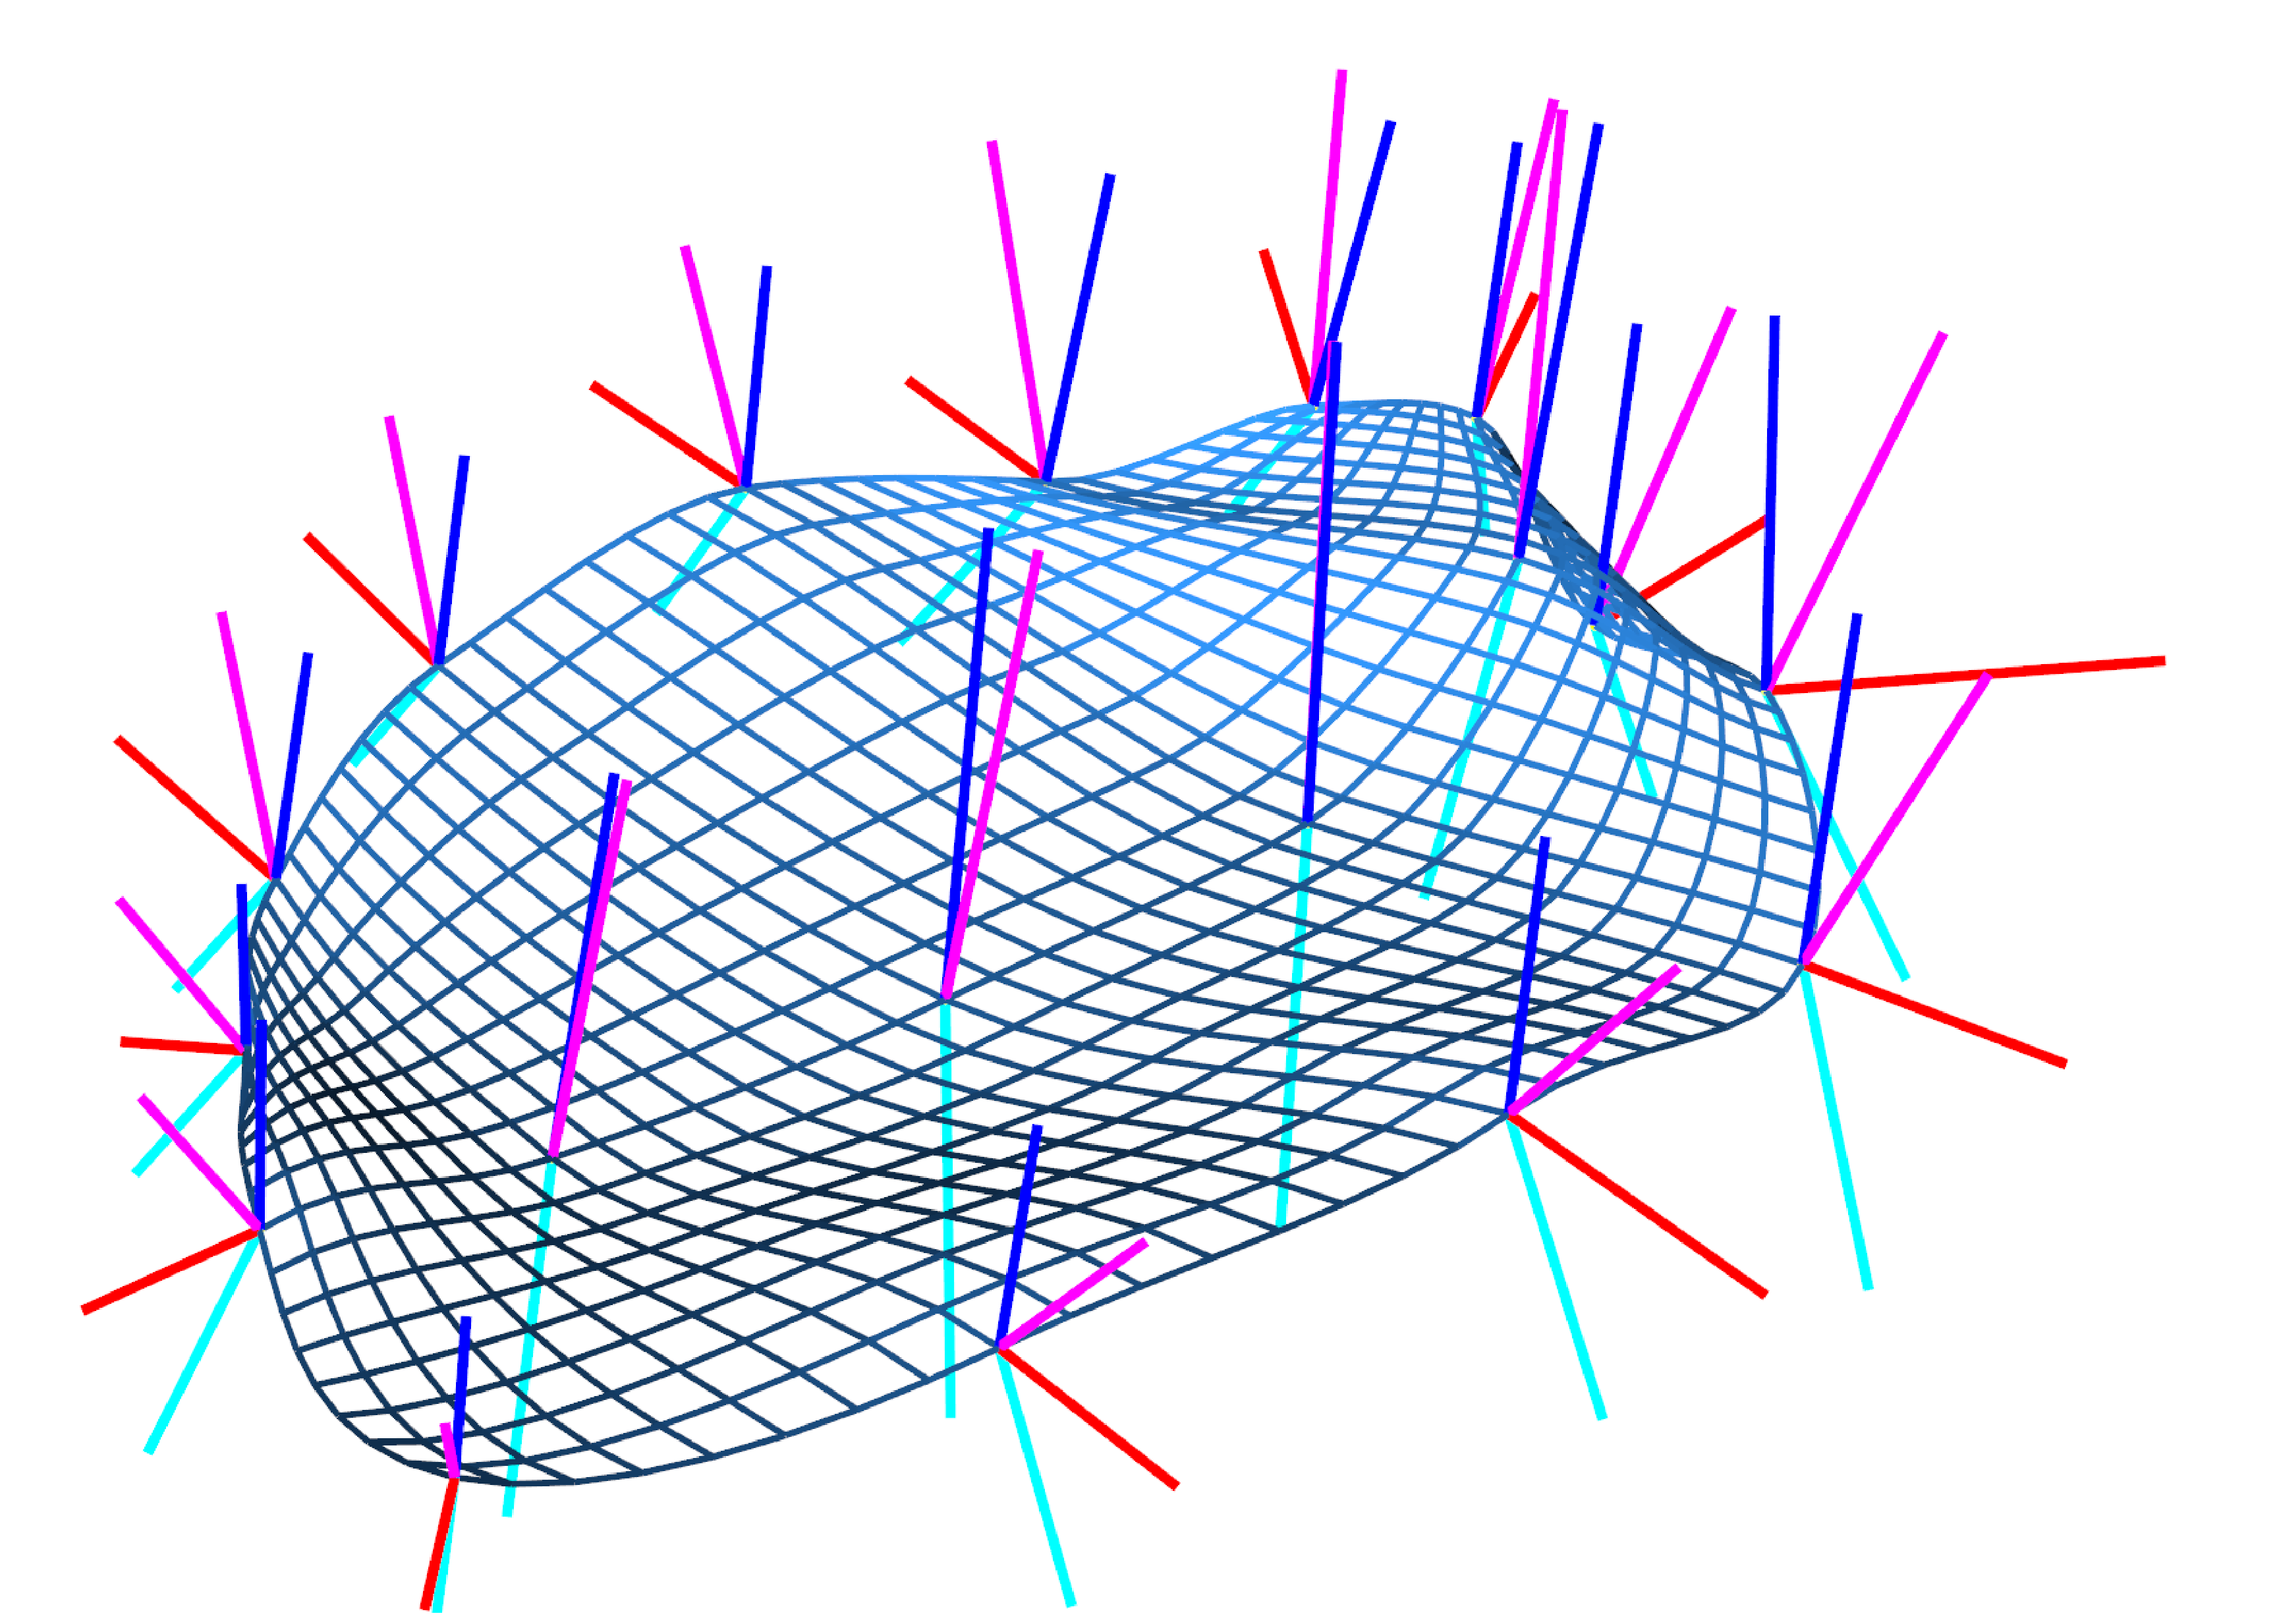
\epsfig{file = interpolationMedialSheet3, width =7cm}}
 \caption[Slab's MS interpolation.]{MS interpolation for a slab type s-rep. The top spoke is shown in magenta, the bottom spoke in cyan, the crest spoke in red,
          the MS is shown in light blue and the normal to the sheet is shown in blue.}
 \label{fig:interpolationMedialSheet}  
\end{figure}

\begin{equation}
 H_{control} = \left [ \begin{array}{cccc}
                    p_{11} & p_{12} 			& \partial p_{{11}_v}^T & \partial p_{{12}_v}^T \\
                    p_{21} & p_{22}			& \partial p_{{21}_v}^T & \partial p_{{22}_v}^T \\
                    \partial p_{{11}_u}^T & \partial p_{{12}_u}^T	& h_{0} & h_{0} \\
                    \partial p_{{21}_u}^T & \partial p_{{22}_u}^T	& h_{0} & h_{0} \\
                    
                   \end{array} \right ]
  \label{equ:hermiteControl}
\end{equation}

To interpolate the SS, a Hermite matrix patch is defined in equation \ref{equ:hermiteControl},
where $\partial p(u,v)^T = \partial p(u,v) - (\partial p(u,v) \cdot N(u, v))N(u,v)$ is the projection of the discrete derivatives in directions $u$ or $v$ onto the tangent planes
that are determined by the normals $N(u,v)$, so the MS interpolation depends on the normals and the discrete derivatives; $h_{0}$ is a vector filled with $0$. 

\begin{equation}
 \begin{array}{l}
  H_1(s)= 2s^3 - 3s^2 + 1\\
  H_2(s)= -2s^3 + 3s^2\\
  H_3(s)= s^3 - 2s^2 + s\\
  H_4(s)= s^3 - s^2\\
 \end{array}
\label{equ:weightFunctions}
\end{equation}

\begin{equation}
 p(u, v) = \left [ \begin{array}{cccc} H_1(\hat u) & H_2(\hat u) & H_3(\hat u) & H_4(\hat u) \end{array} \right ]
                H_{control}
           \left [ \begin{array}{c} H_1(\hat v) \\
				     H_2(\hat v) \\ 
				     H_3(\hat v) \\ 
				     H_4(\hat v) 
		    \end{array} \right ]
\label{equ:interpolatedPoint}
\end{equation}

The interpolated position for any atom on the SS is shown in equation \ref{equ:interpolatedPoint}, 
using a Hermite matrix control patch and the weight functions defined in \ref{equ:weightFunctions}.
$\hat u = (u - floor(u))/\Delta u$, where $floor(u)$ returns the $u$ coordinate of the atom at $p_{11}$,
similarly for $\hat v$, notice that every patch is interpolated by varying $(\hat u, \hat v): 0 \rightarrow 1$.
Figure \ref{fig:interpolationMedialSheet} shows the interpolation of the MS at different levels for the same figure.

In a similar manner, the spoke interpolation can be done using Hermite basis functions. Instead of using the control points
$p(u, v)$, the spokes $S(u, v)$ are used. Accordingly, the discrete derivatives are computed for each spoke, the difference
in this case is that no projection is done using the normals to the SS; the spoke interpolation only depends on the discrete derivatives. 


\begin{figure} 
 \centering  
 \subfigure[Interpolated spokes]{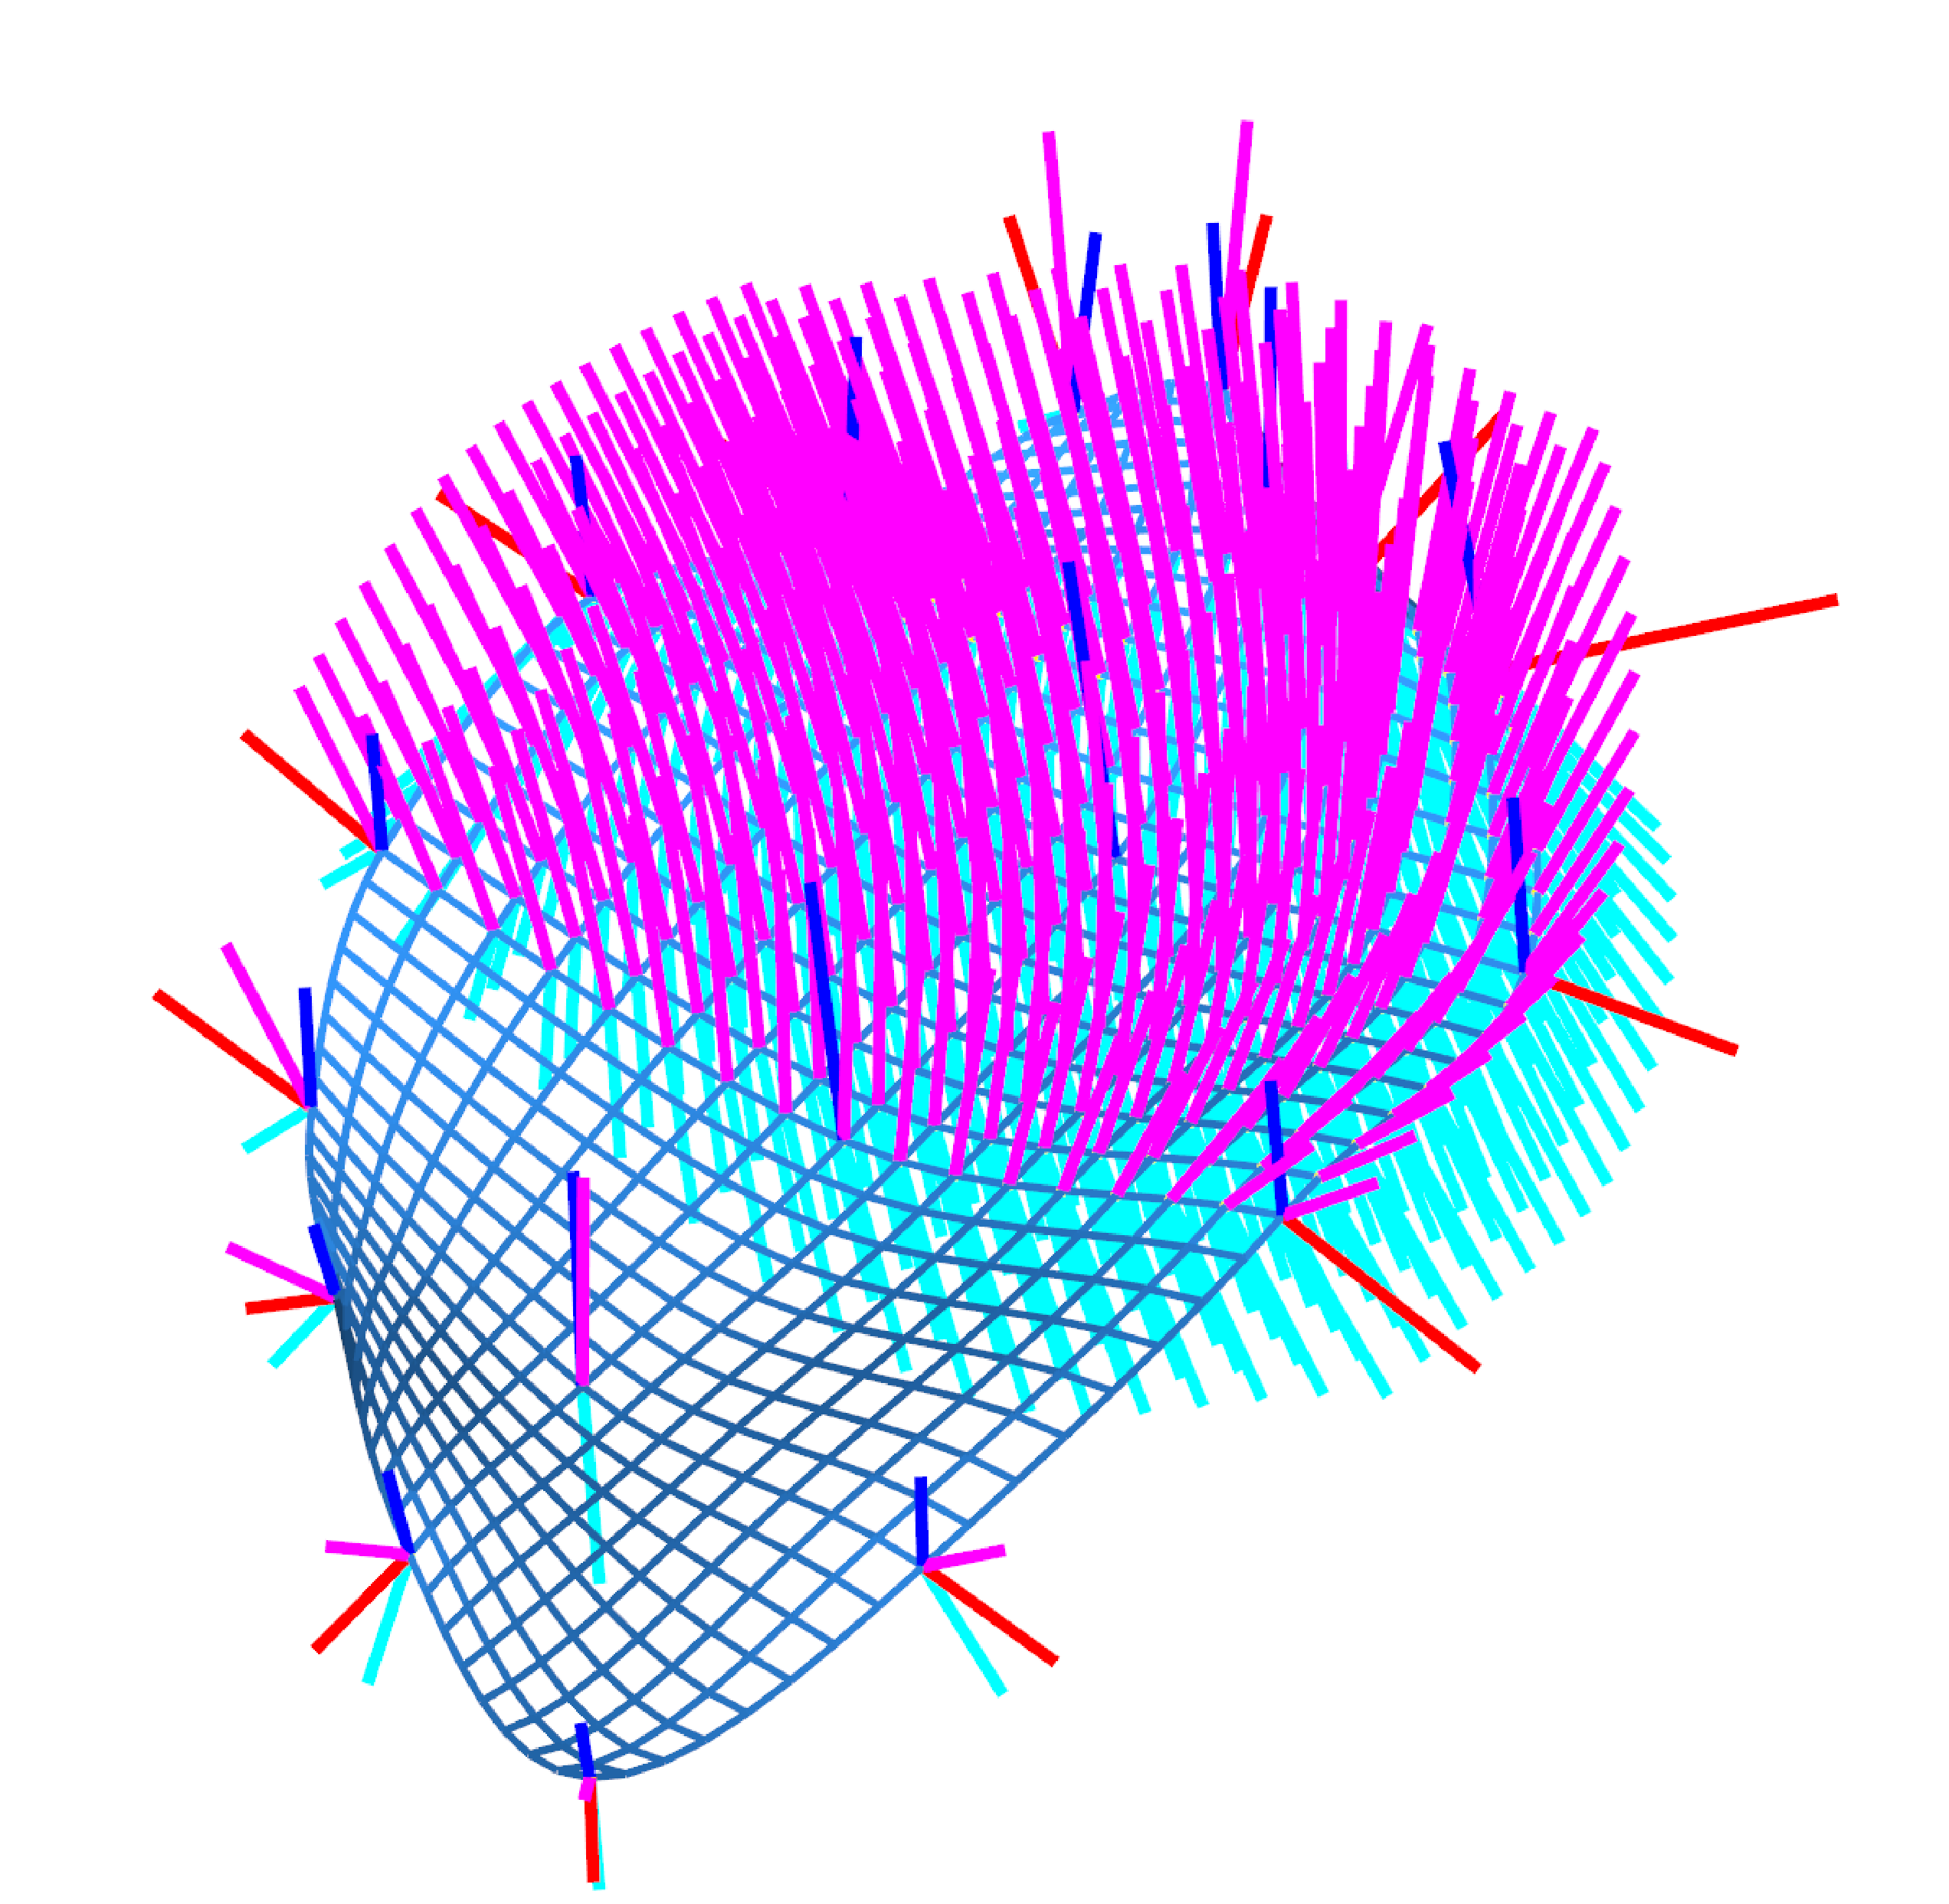
\epsfig{file = interpolationSpokes.eps, width = 7cm} }
 \subfigure[Union of spoke tips]{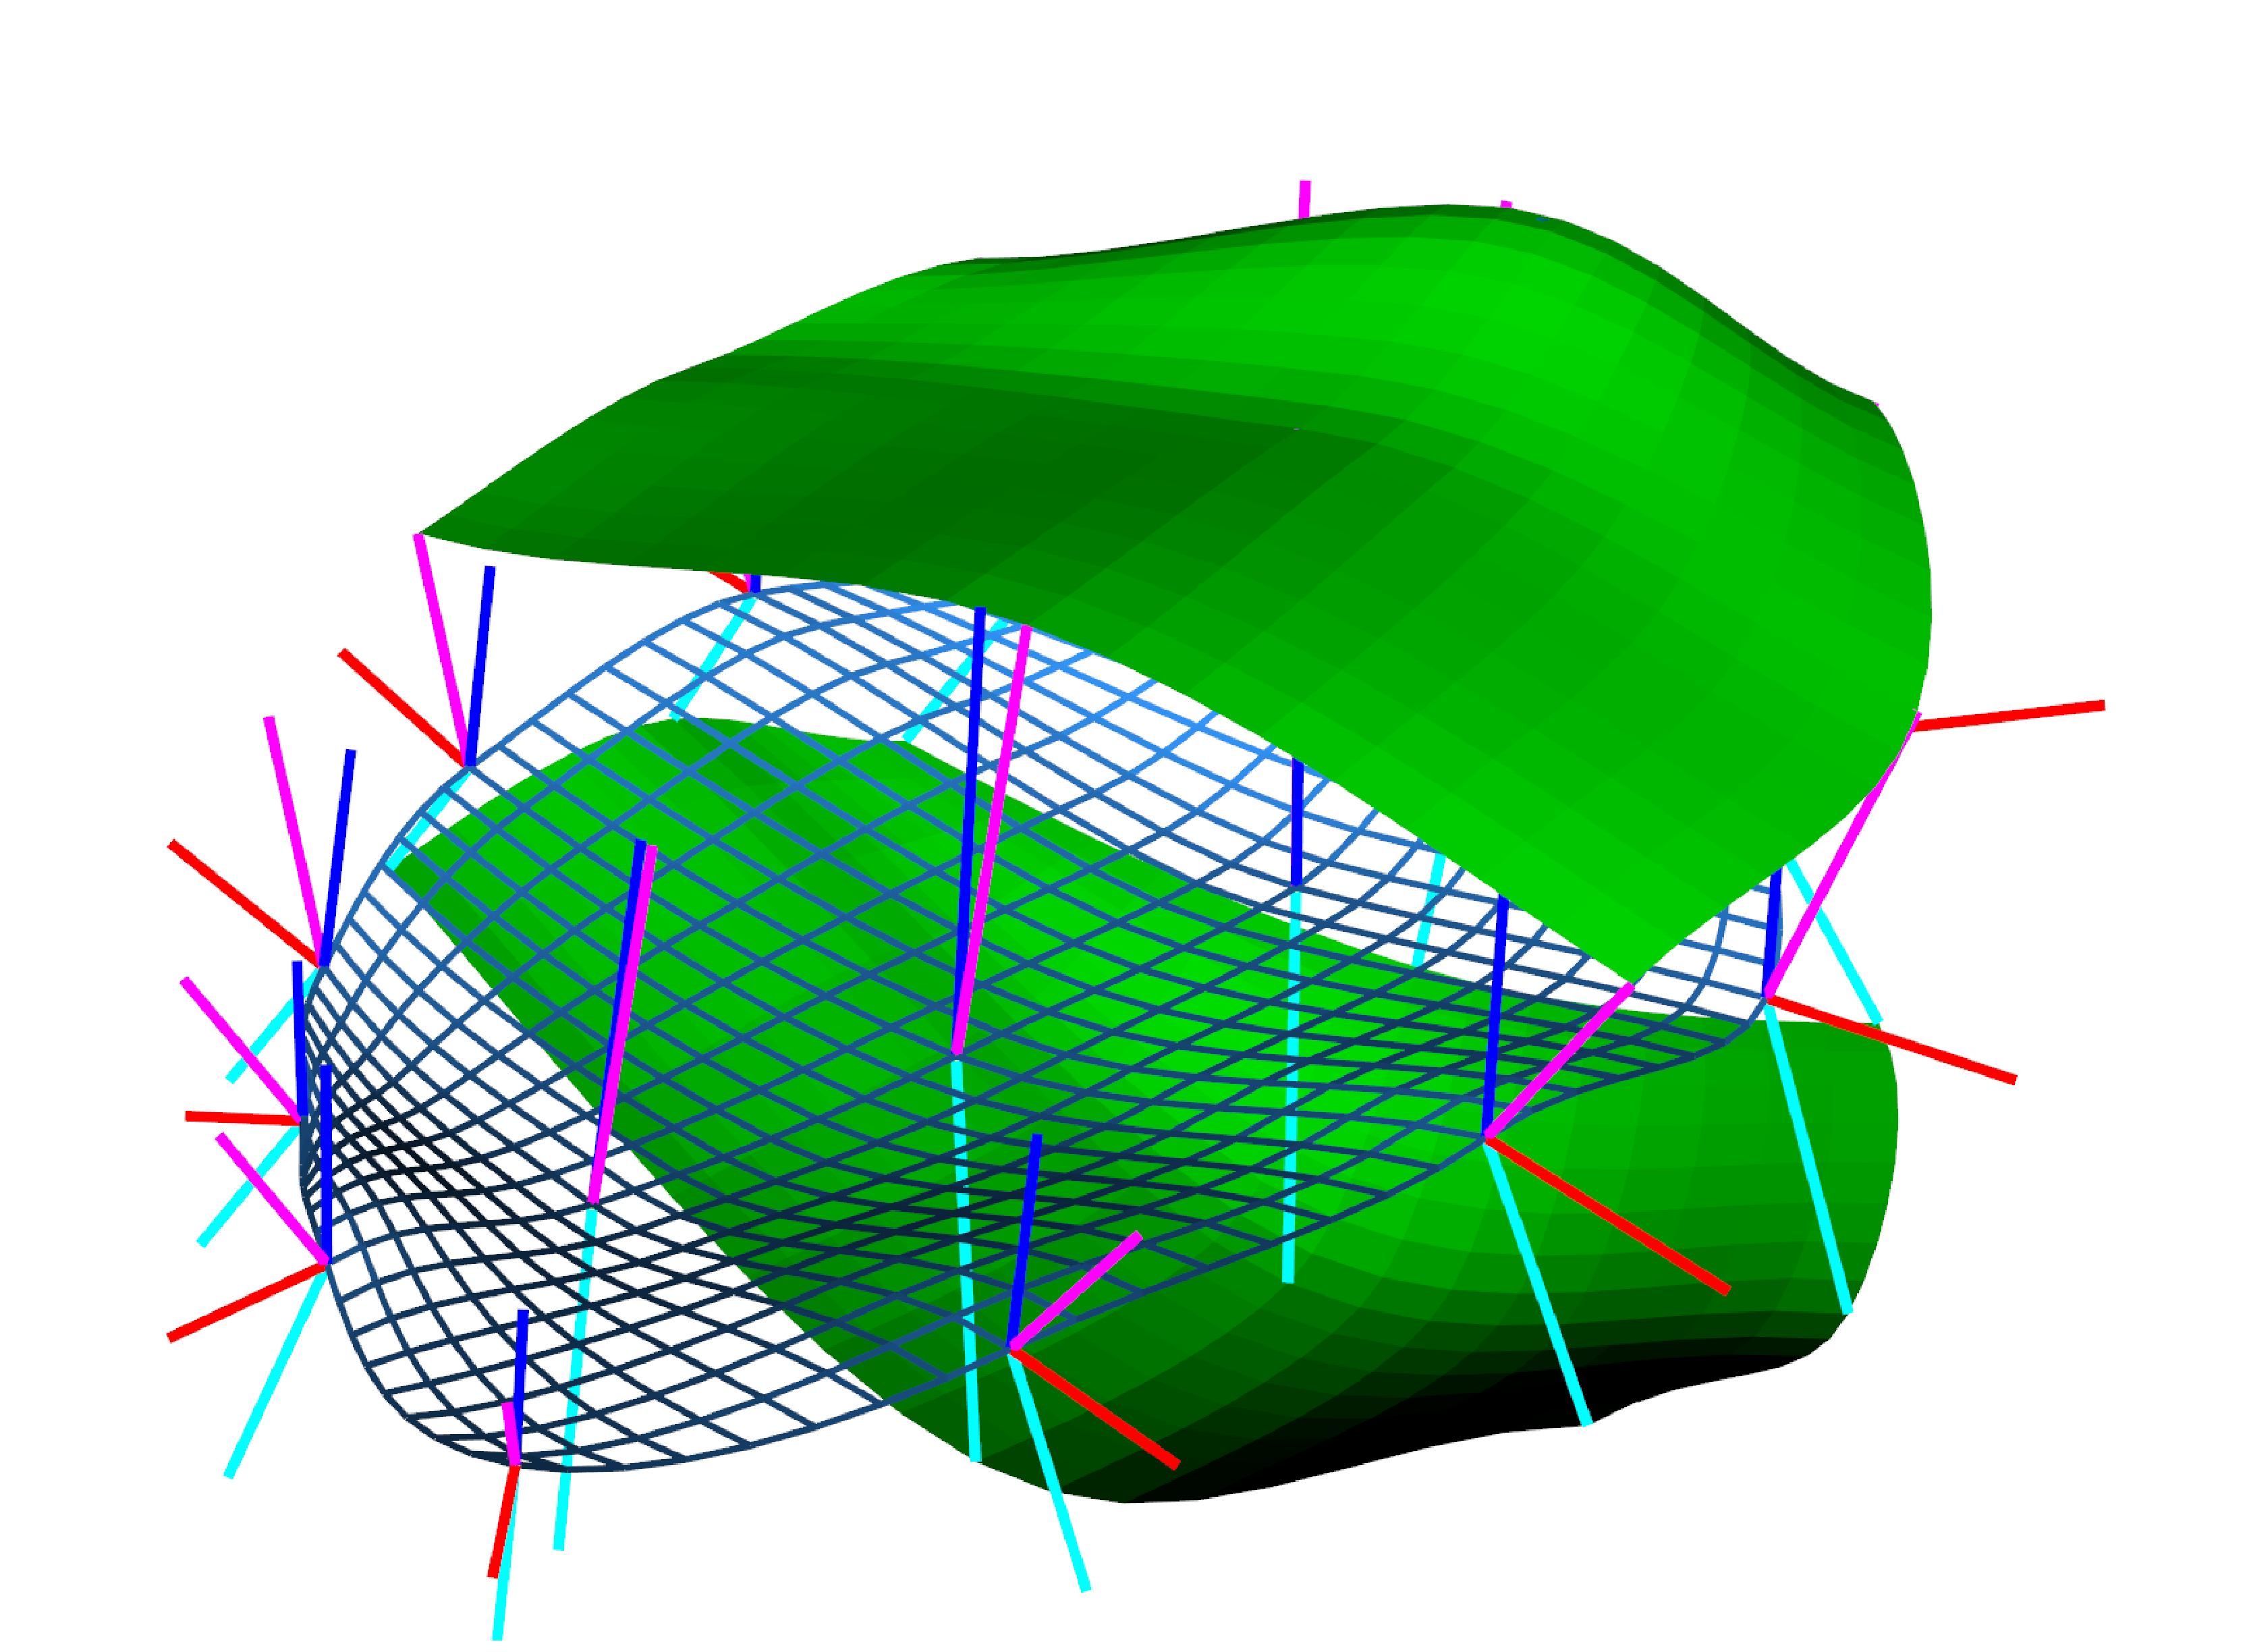
\epsfig{file = interpolationSurface3.eps, width = 7cm}}
 \caption[Top and bottom surface interpolation.]{Top and bottom surfaces interpolated for a given atom. The surfaces are generated from the spoke interpolation.}
 \label{fig:GeneratedSurfaceSpokeInterpolation}  
\end{figure}

The top and bottom surface can be generated using the mechanisms described above. 
Figure \ref{fig:GeneratedSurfaceSpokeInterpolation} shows the implied surface generated by the union of 
interpolated spoke tips.
As mentioned before, both surfaces meet at the crest of the object, 
Section \ref{sec:crestInterpolation} explains how to perform the crest interpolation which 
can also be used to interpolate tubular figures.

\subsection{Crest interpolation}
\label{sec:crestInterpolation}

For the crest interpolation, we wish to fit a surface that 
does not collapse towards the interior of the object. In other words, 
its cross-section should be convex
in the principal direction and preserve $C^2$ continuity. Another property of the surface is that the directional 
derivatives computed for every spoke should be matched in order to produce a smooth surface
to the Hermite based interpolation previously explained.

The crest interpolation method is explained by showing how to interpolate the lenghts $r$ of a spoke
that sweeps according to an angle $\theta$.
The function $r(\theta)$ returns the lenght at a given angle.
In a similar way, we wish to interpolate the cross-section in the crest, where theta 
runs between the terminus of the top or bottom spoke to the crest spoke. 

The same problem can be extended to 3 dimensions where the interpolation produces a space curve.
In order to produce an interpolated surface the interpolation of the cross-section 
sweeps along the skeletal sheet.

\begin{equation} 
 \frac{\partial^2 r(\theta)}{\partial \theta} = q_0  +  q_1  \theta + q_2  \theta^2  
 \label{equ:curvature}
\end{equation}

The first step is to define a quadratic function of the curvature, as shown in Equation
\ref{equ:curvature}, we would like to enforce convexity in the interpolated curve.
By integrating this equation twice, we find the function that gives us the length for $\theta \in [0, \theta_{max}]$.

\begin{eqnarray} 
  \frac{\partial r(\theta)}{\partial \theta} &=& \int_0^{\theta_{max}} \frac{\partial^2 r(\theta)}{\partial \theta} \partial \theta \\
  \frac{\partial r(\theta)}{\partial \theta} &=& \frac{\partial r_0}{\partial \theta} + q_0  \theta + \frac{1}{2}  q_1  \theta^2 + \frac{1}{3}  q_2  \theta^3  \\
  r(\theta) &=& \int_0^{\theta_{max}} \frac{\partial r(\theta)}{\partial \theta} \partial \theta \\
  r(\theta) &=& r_0 + \frac{\partial r_0}{\partial \theta}  \theta + \frac{1}{2}  q_0  \theta^2 + \frac{1}{6}  q_1  \theta^3 + \frac{1}{12}  q_2  \theta^4  
\end{eqnarray}

We start by solving for coefficients $q_1$ and $q_2$,
using the system of equations $r(\theta)$, $\partial r(\theta)/\partial \theta$ and $\partial^2 r(\theta)/\partial \theta$, 
as shown in equation \ref{equ:solveQ1}.

\begin{eqnarray} 
q_2 &=& \frac{6}{\theta_{max}^4} (2 \partial r_{end} \theta_{max} + q_0 \theta_{max}^2 - 6 r_{end} + 6 r_0 + 4 \partial r_0 \theta_{max}) \\
q_1 &=& \frac{-6}{\theta_{max}^3} (-\partial r_{end} + r_0 + \partial r_0 \theta_{max} +  \frac{q_0}{2} \theta_{max} + \frac{q_2}{12} \theta_{max}^4)
\label{equ:solveQ1}
\end{eqnarray} 

There exists a solution to the problem for every $q_0$ but
the optimal solution is found when $q_0$ minimizes the average 2nd derivative
of $r$ as shown in Equation \ref{equ:minimizeCurvature}.

\begin{equation}
 \partial r_{end} =  -1 \partial r_{end} = 0 \partial r_{end} = 1 r_0 \theta \partial r_0
\end{equation}


\begin{equation}  
  \hat q_0 = \operatorname*{arg\,min}_{q_0} \sum_{\theta = 0}^{\theta_{max}} \frac{\partial^2 r(\theta)}{\partial \theta}
  \label{equ:minimizeCurvature}
\end{equation}

Notice that the parameters $r_0$, $r_{end}$, $\partial r_0$ and $\partial r_{end}$ correspond to 
initial and final lengths, and rates of the change at $r_0$ and $r_{end}$ respectively.

\begin{figure} 
 \centering  
 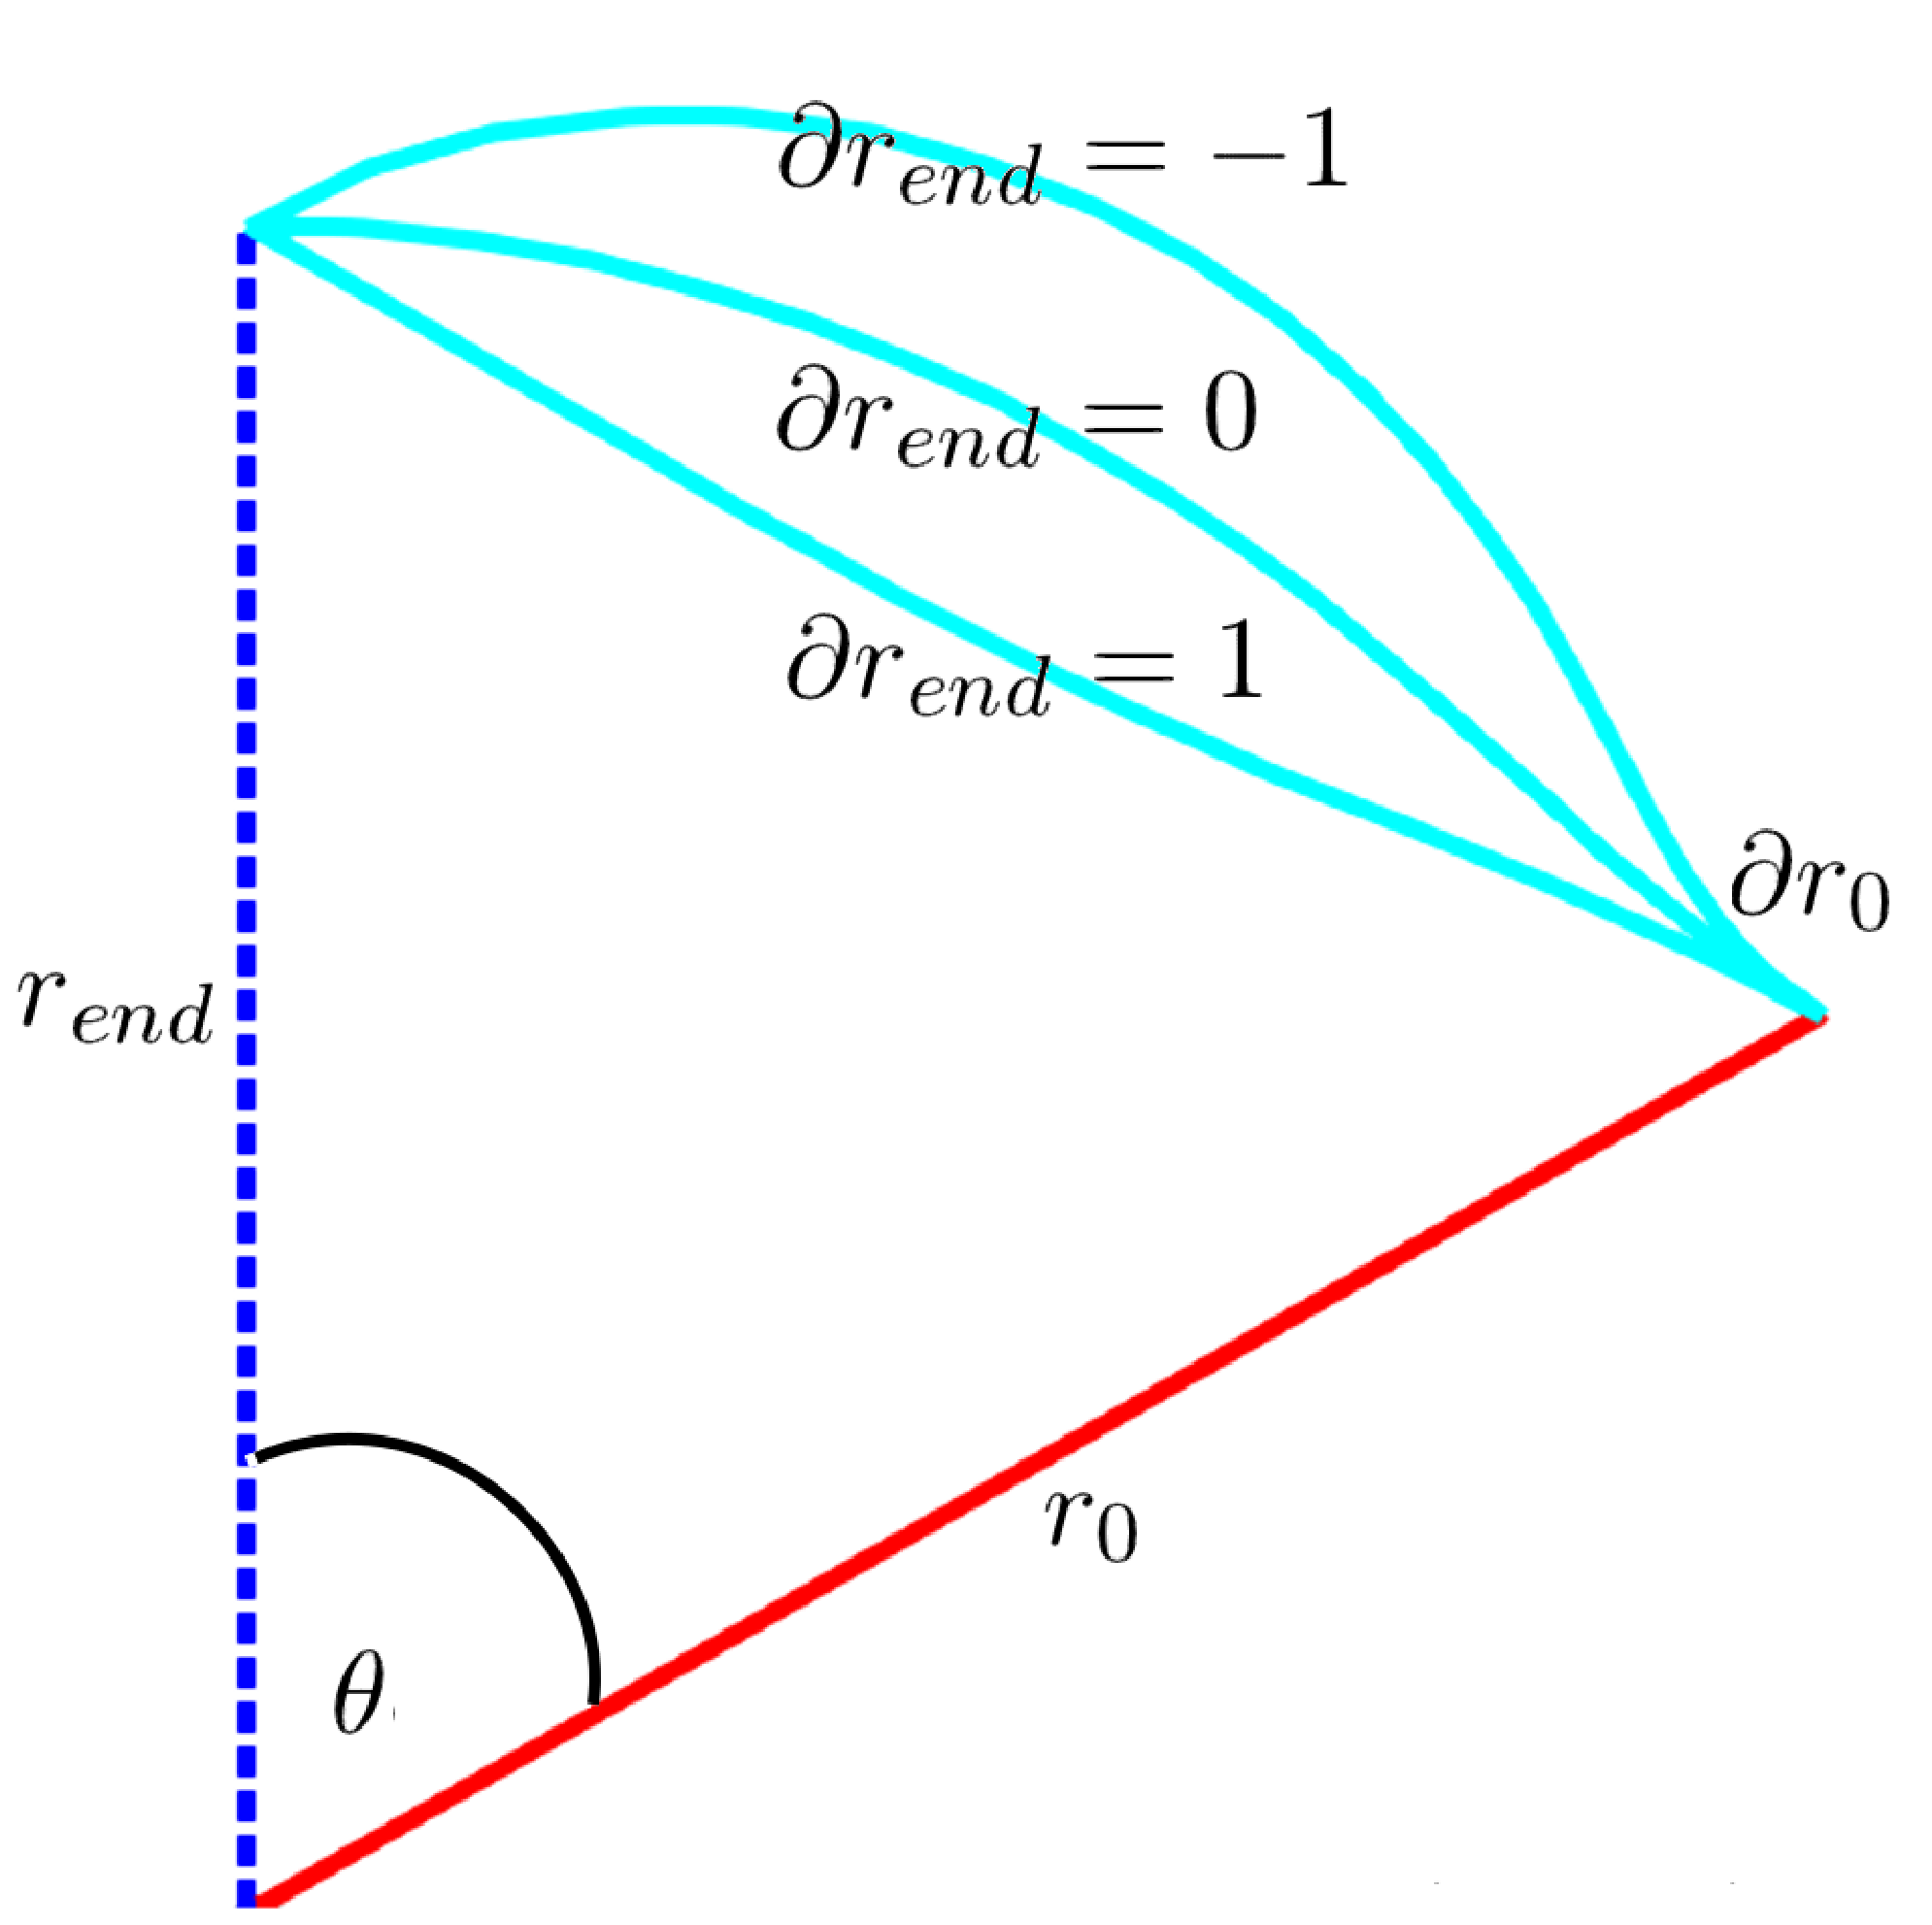
\epsfig{file = interpolationCrest0.eps, width =8cm}
 \caption[Radius interpolation.]{Radius interpolation showing the result for different $\partial r_{end}$.}
 \label{fig:interpolateRadius}  
\end{figure}

To produce space curves, the fitting is done for $[x, y, z]$ separately.
Using the discrete information given by the s-rep,
it is possible to retrieve $p_0$, $p_{end}$, and compute the discrete derivatives $\partial p_0$, and $\partial p_{end}$ 
which are the parameters to produce the fit.
To produce the crest curve, the crest atoms are considered to be on a loop 
where the crest positions are given by $cp_n$ where $n$ is the number of crest positions.
The directional derivatives are calculated as $\partial cp_j = (cp_{j + 1} - cp_{j - 1})/2$
which are projected onto the tangent plane given by the SS normal at each atom
$\partial \hat {cp_j} = \partial cp_j - (\partial cp_j \cdot N_{cp_j})N_{cp_j}$.
Figure \ref{fig:crestCurve} shows the interpolated crest as a space curve.

\begin{figure} 
 \centering  
 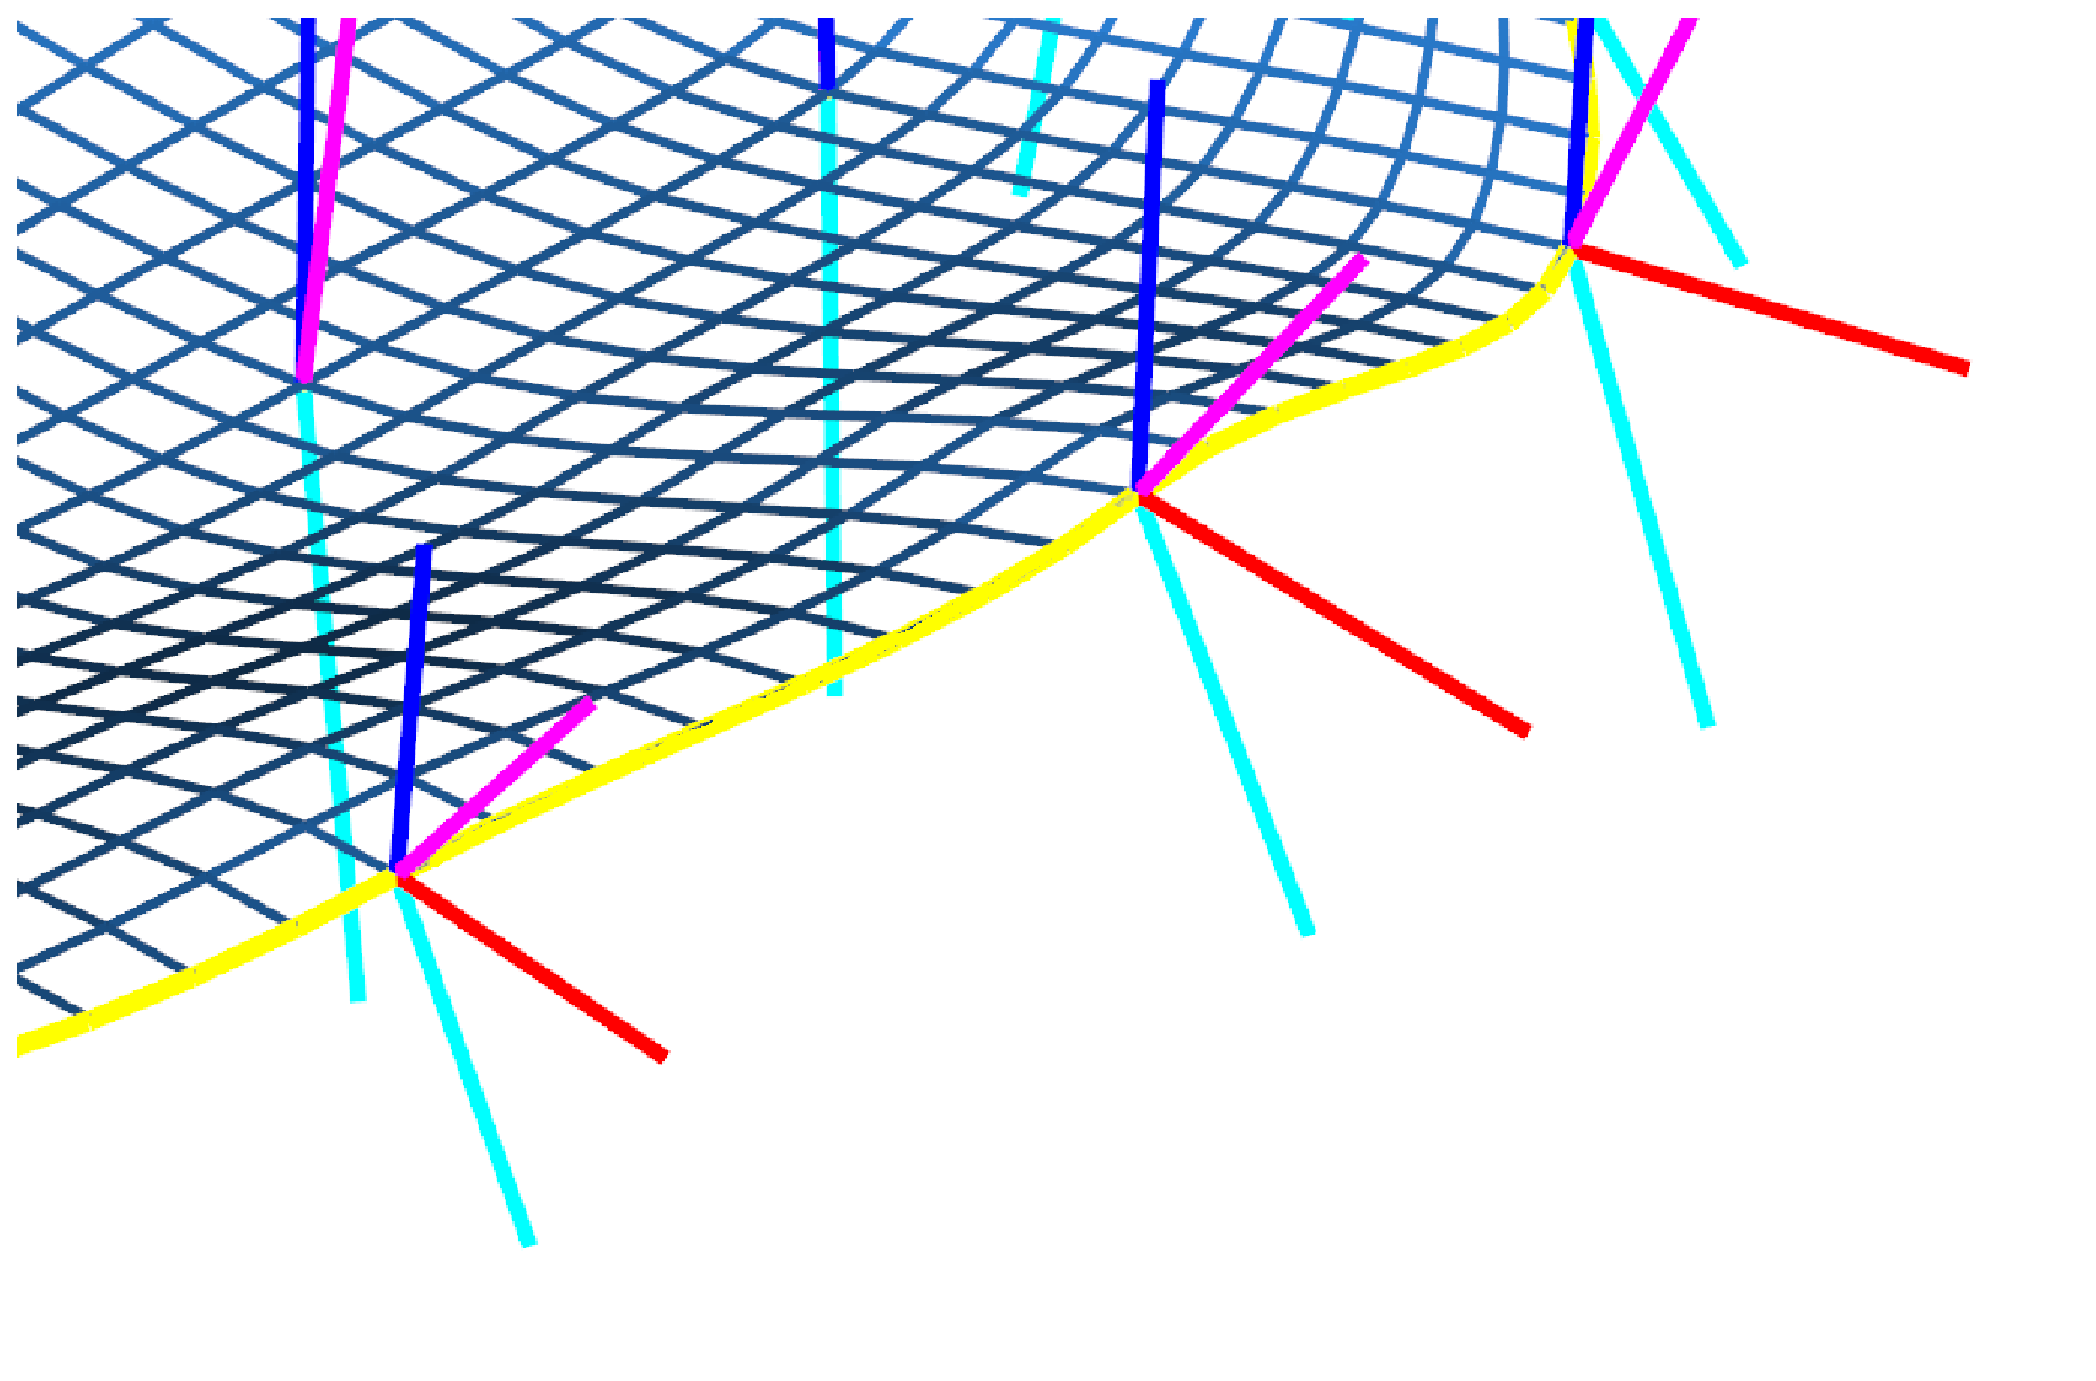
\epsfig{file = interpolationCrestCurve1.eps, width = 8cm}
 \caption[Interpolated crest curve.]{The interpolated crest curve is shown in yellow, using the crest positions to compute the directional derivatives and projecting the derivatives onto the tangent plane.}
 \label{fig:crestCurve}  
\end{figure}

\begin{figure} 
 \centering  
  \subfigure[Crest Spokes Top and Bottom]{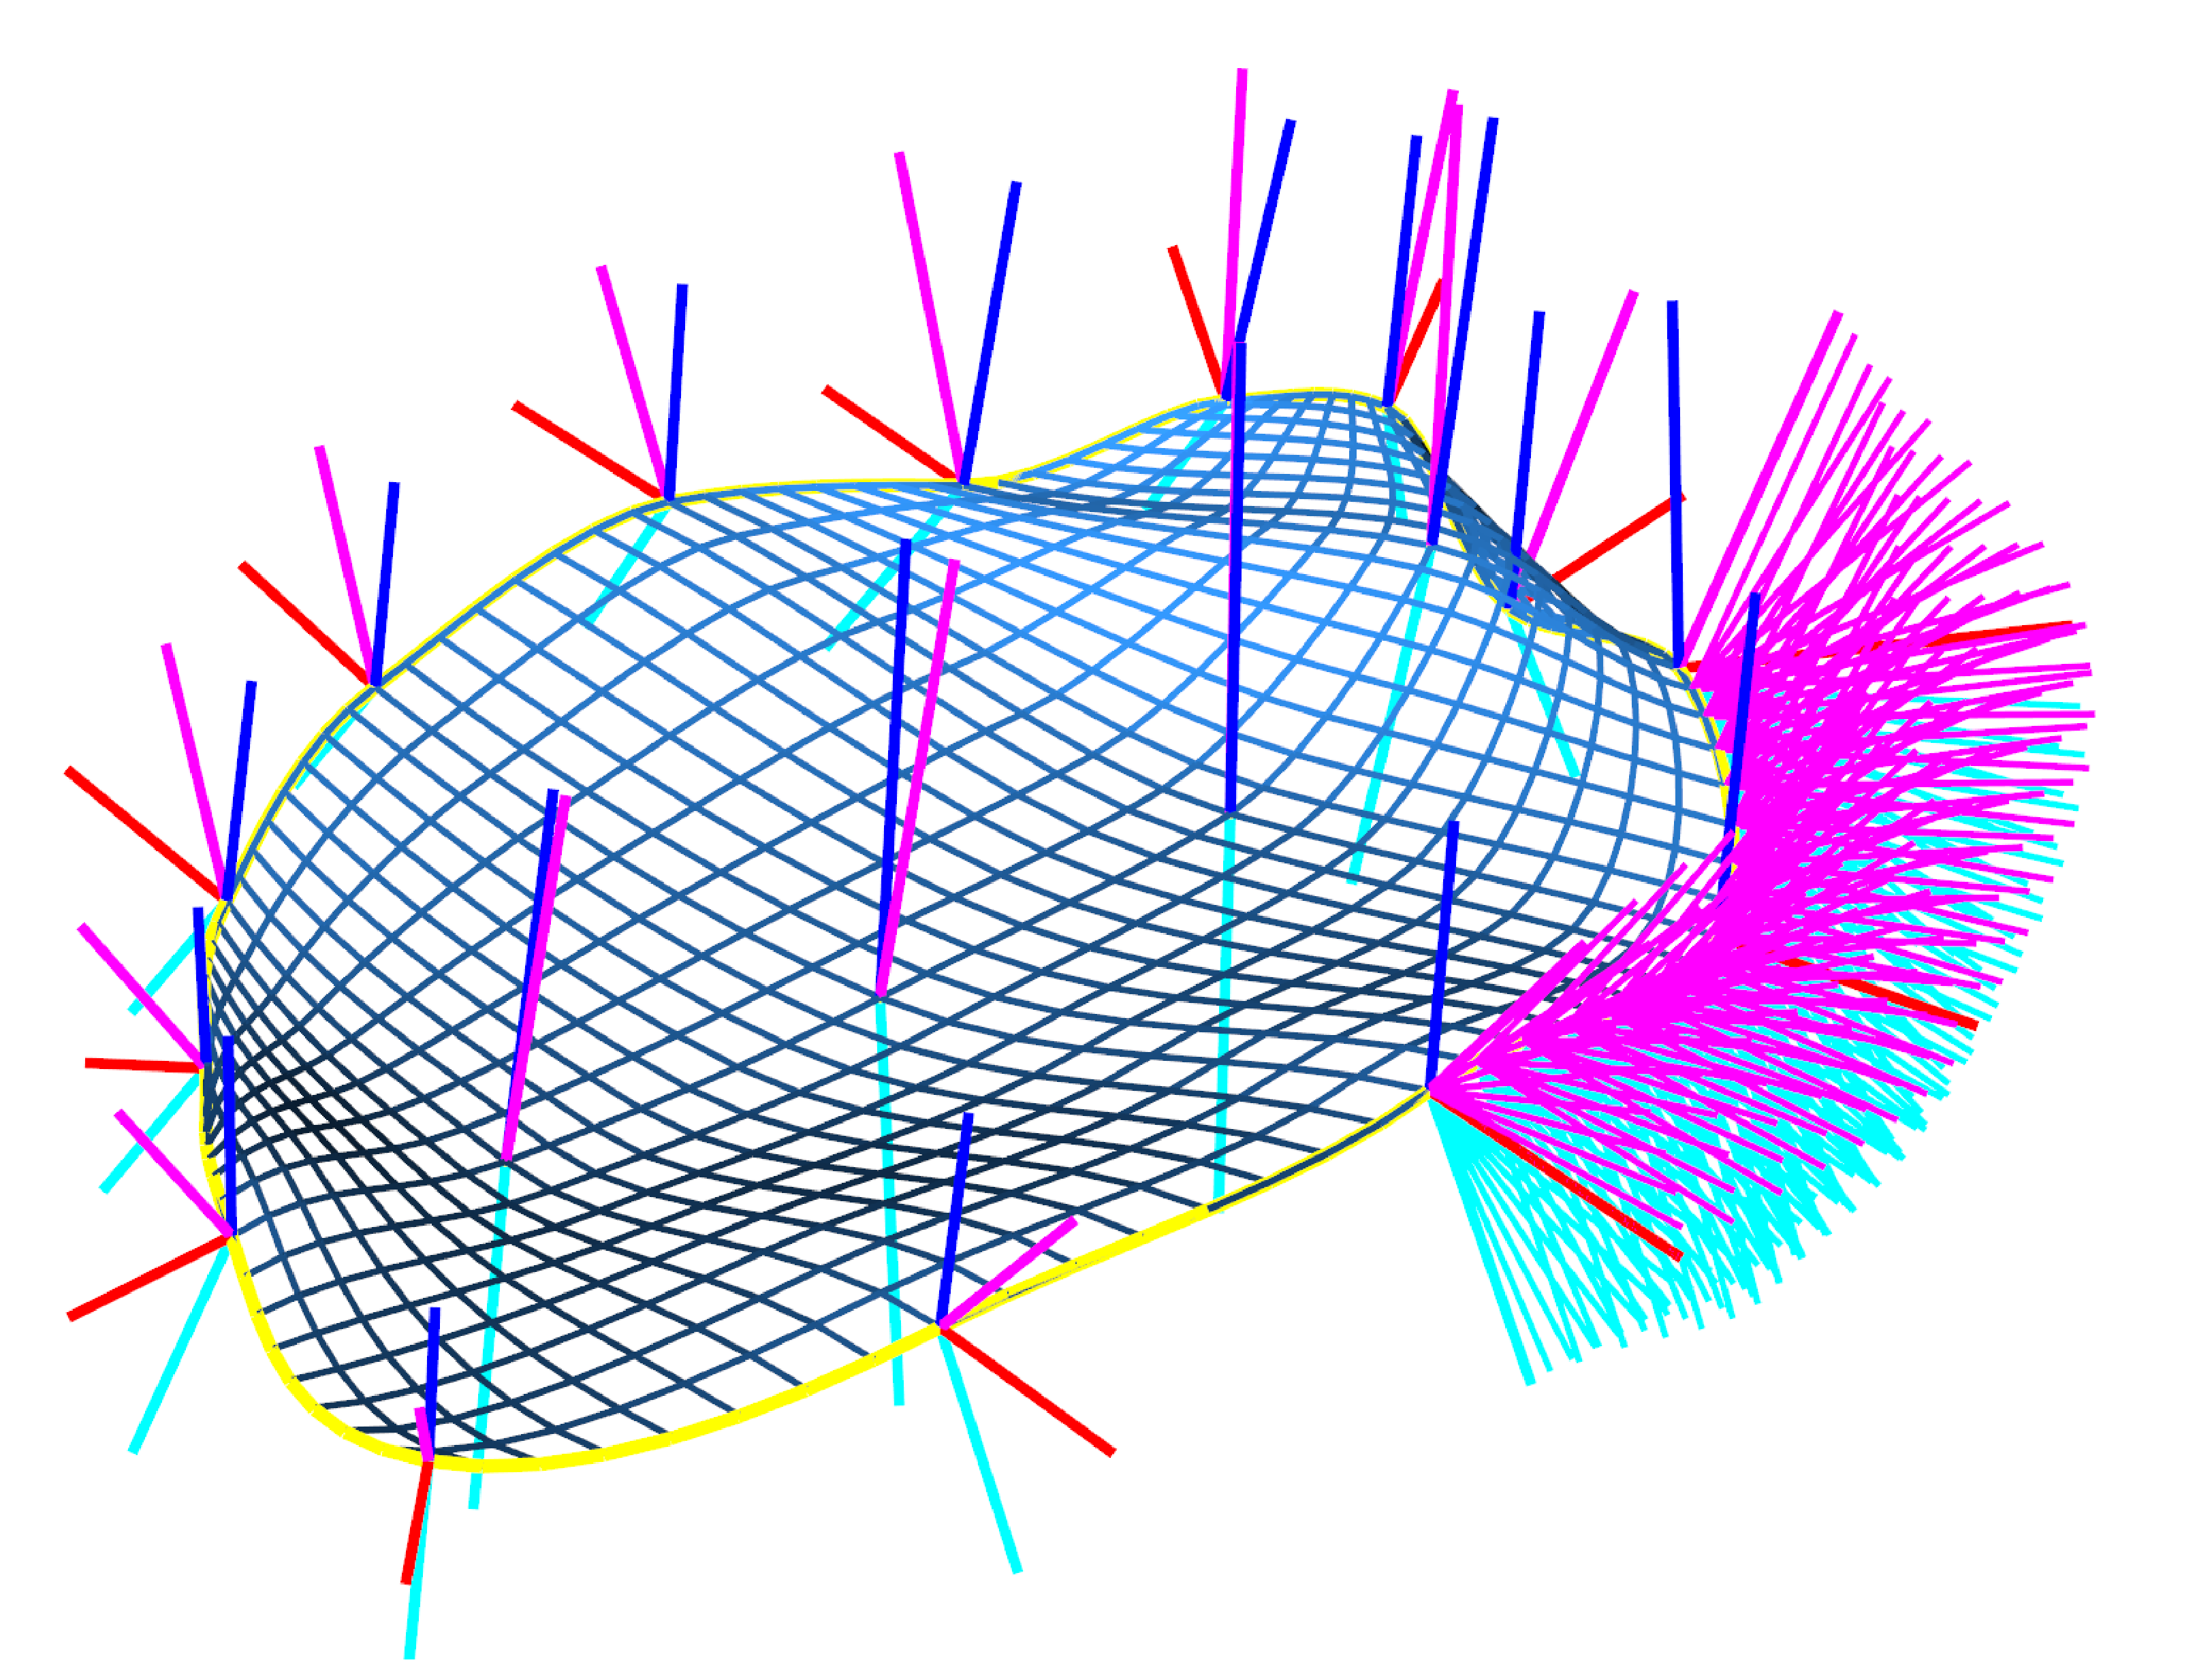
\epsfig{file = interpolationCrestSpokes.eps, width = 7cm}}
  \subfigure[Union of spokes to produce the crest]{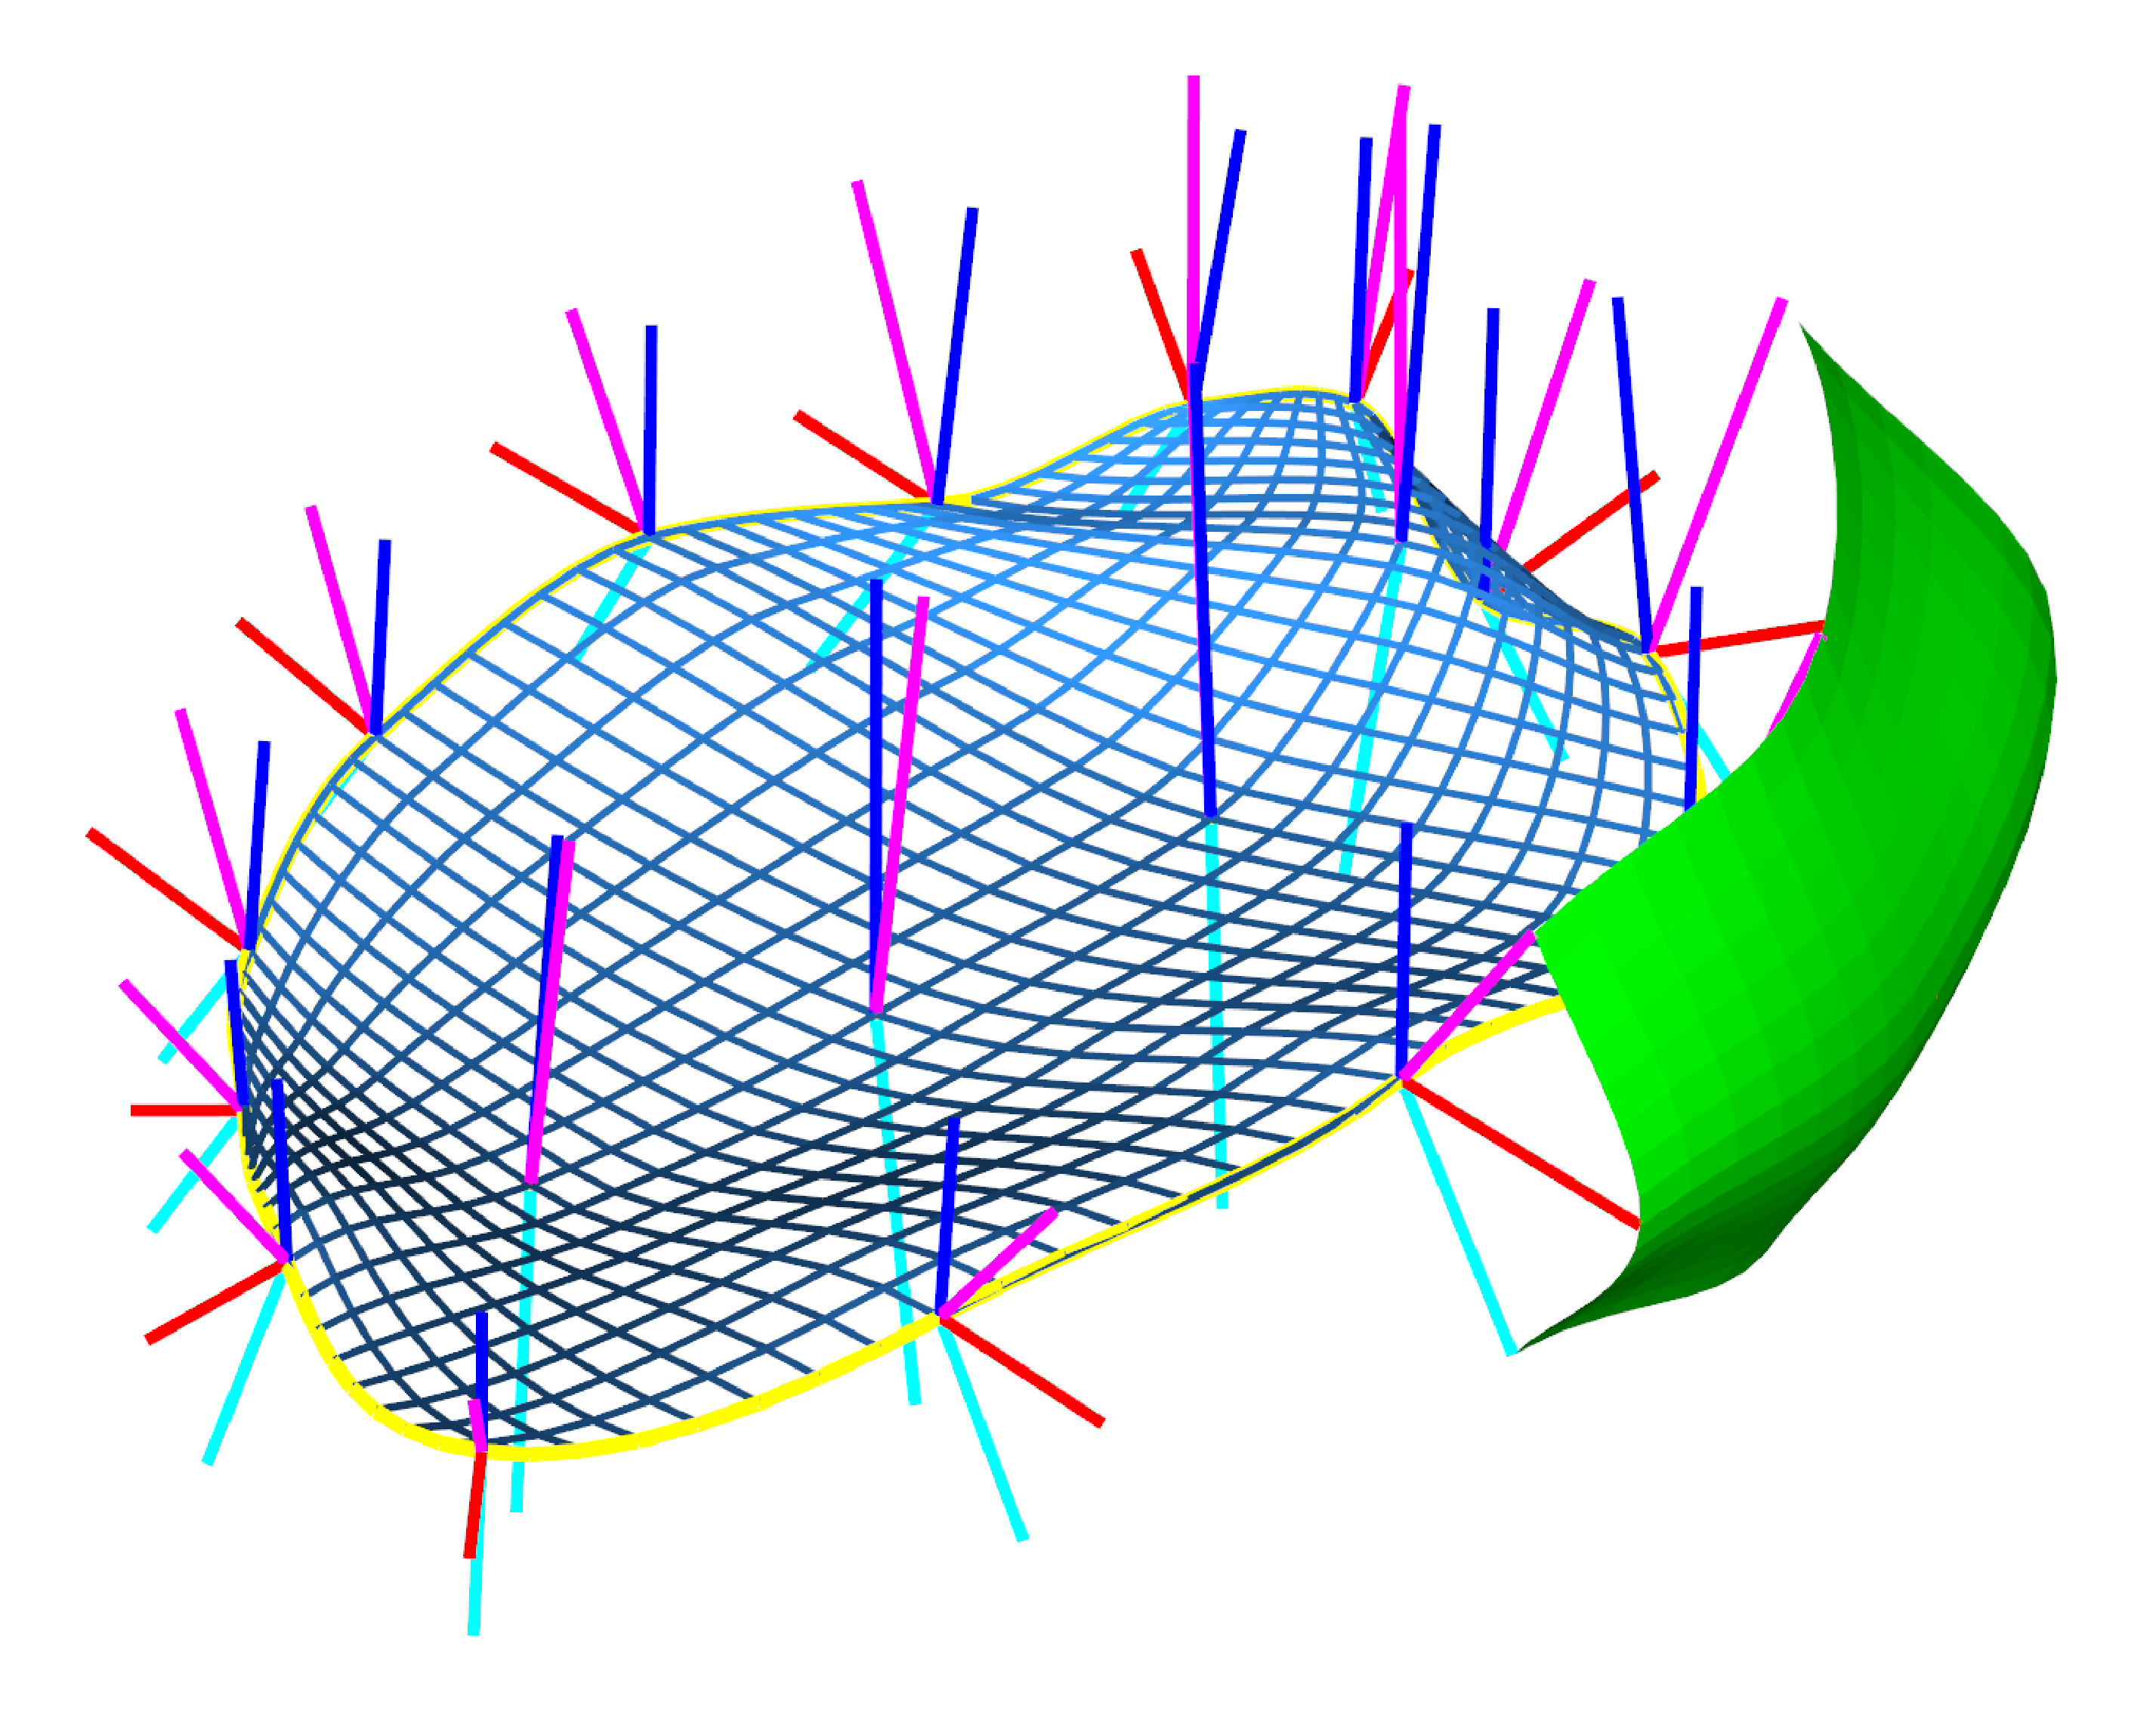
\epsfig{file = interpolationCrestSpokes0.eps, width = 7cm}}
 \caption[Slab's surfaces interpolation.]{The method interpolates top, crest and bottom spokes separately. 
	  A second interpolation is produced using the interpolated top, crest and bottom spokes in order to
	  join both sides of the object at the crest.}
 \label{fig:crestSpokes}  
\end{figure}

The same interpolation mechanism is used for top, crest and bottom spokes,
therefore, for a given $t$, 
it is possible to find the top spoke $CS(t)^1$, the crest spoke $CS(t)^0$ and the bottom spoke $CS(t)^{-1}$ 
plus the space curve to find the positions $Cp(t)$ where $t \in [0, 1]$ goes around 
the whole crest of the object. 

Finally we perform a second interpolation to generate the spokes from $top \rightarrow bottom$, which allows
us to produce the interpolated crest. 
Figure \ref{fig:crestSpokes} shows the interpolated spokes and the union of spokes forming a piece of the crest surface.
Figure \ref{fig:srepInterpolated} shows an example of the interpolated surface 
of an amygdala and the crest that joins both surfaces.

\begin{figure} 
 \centering  
 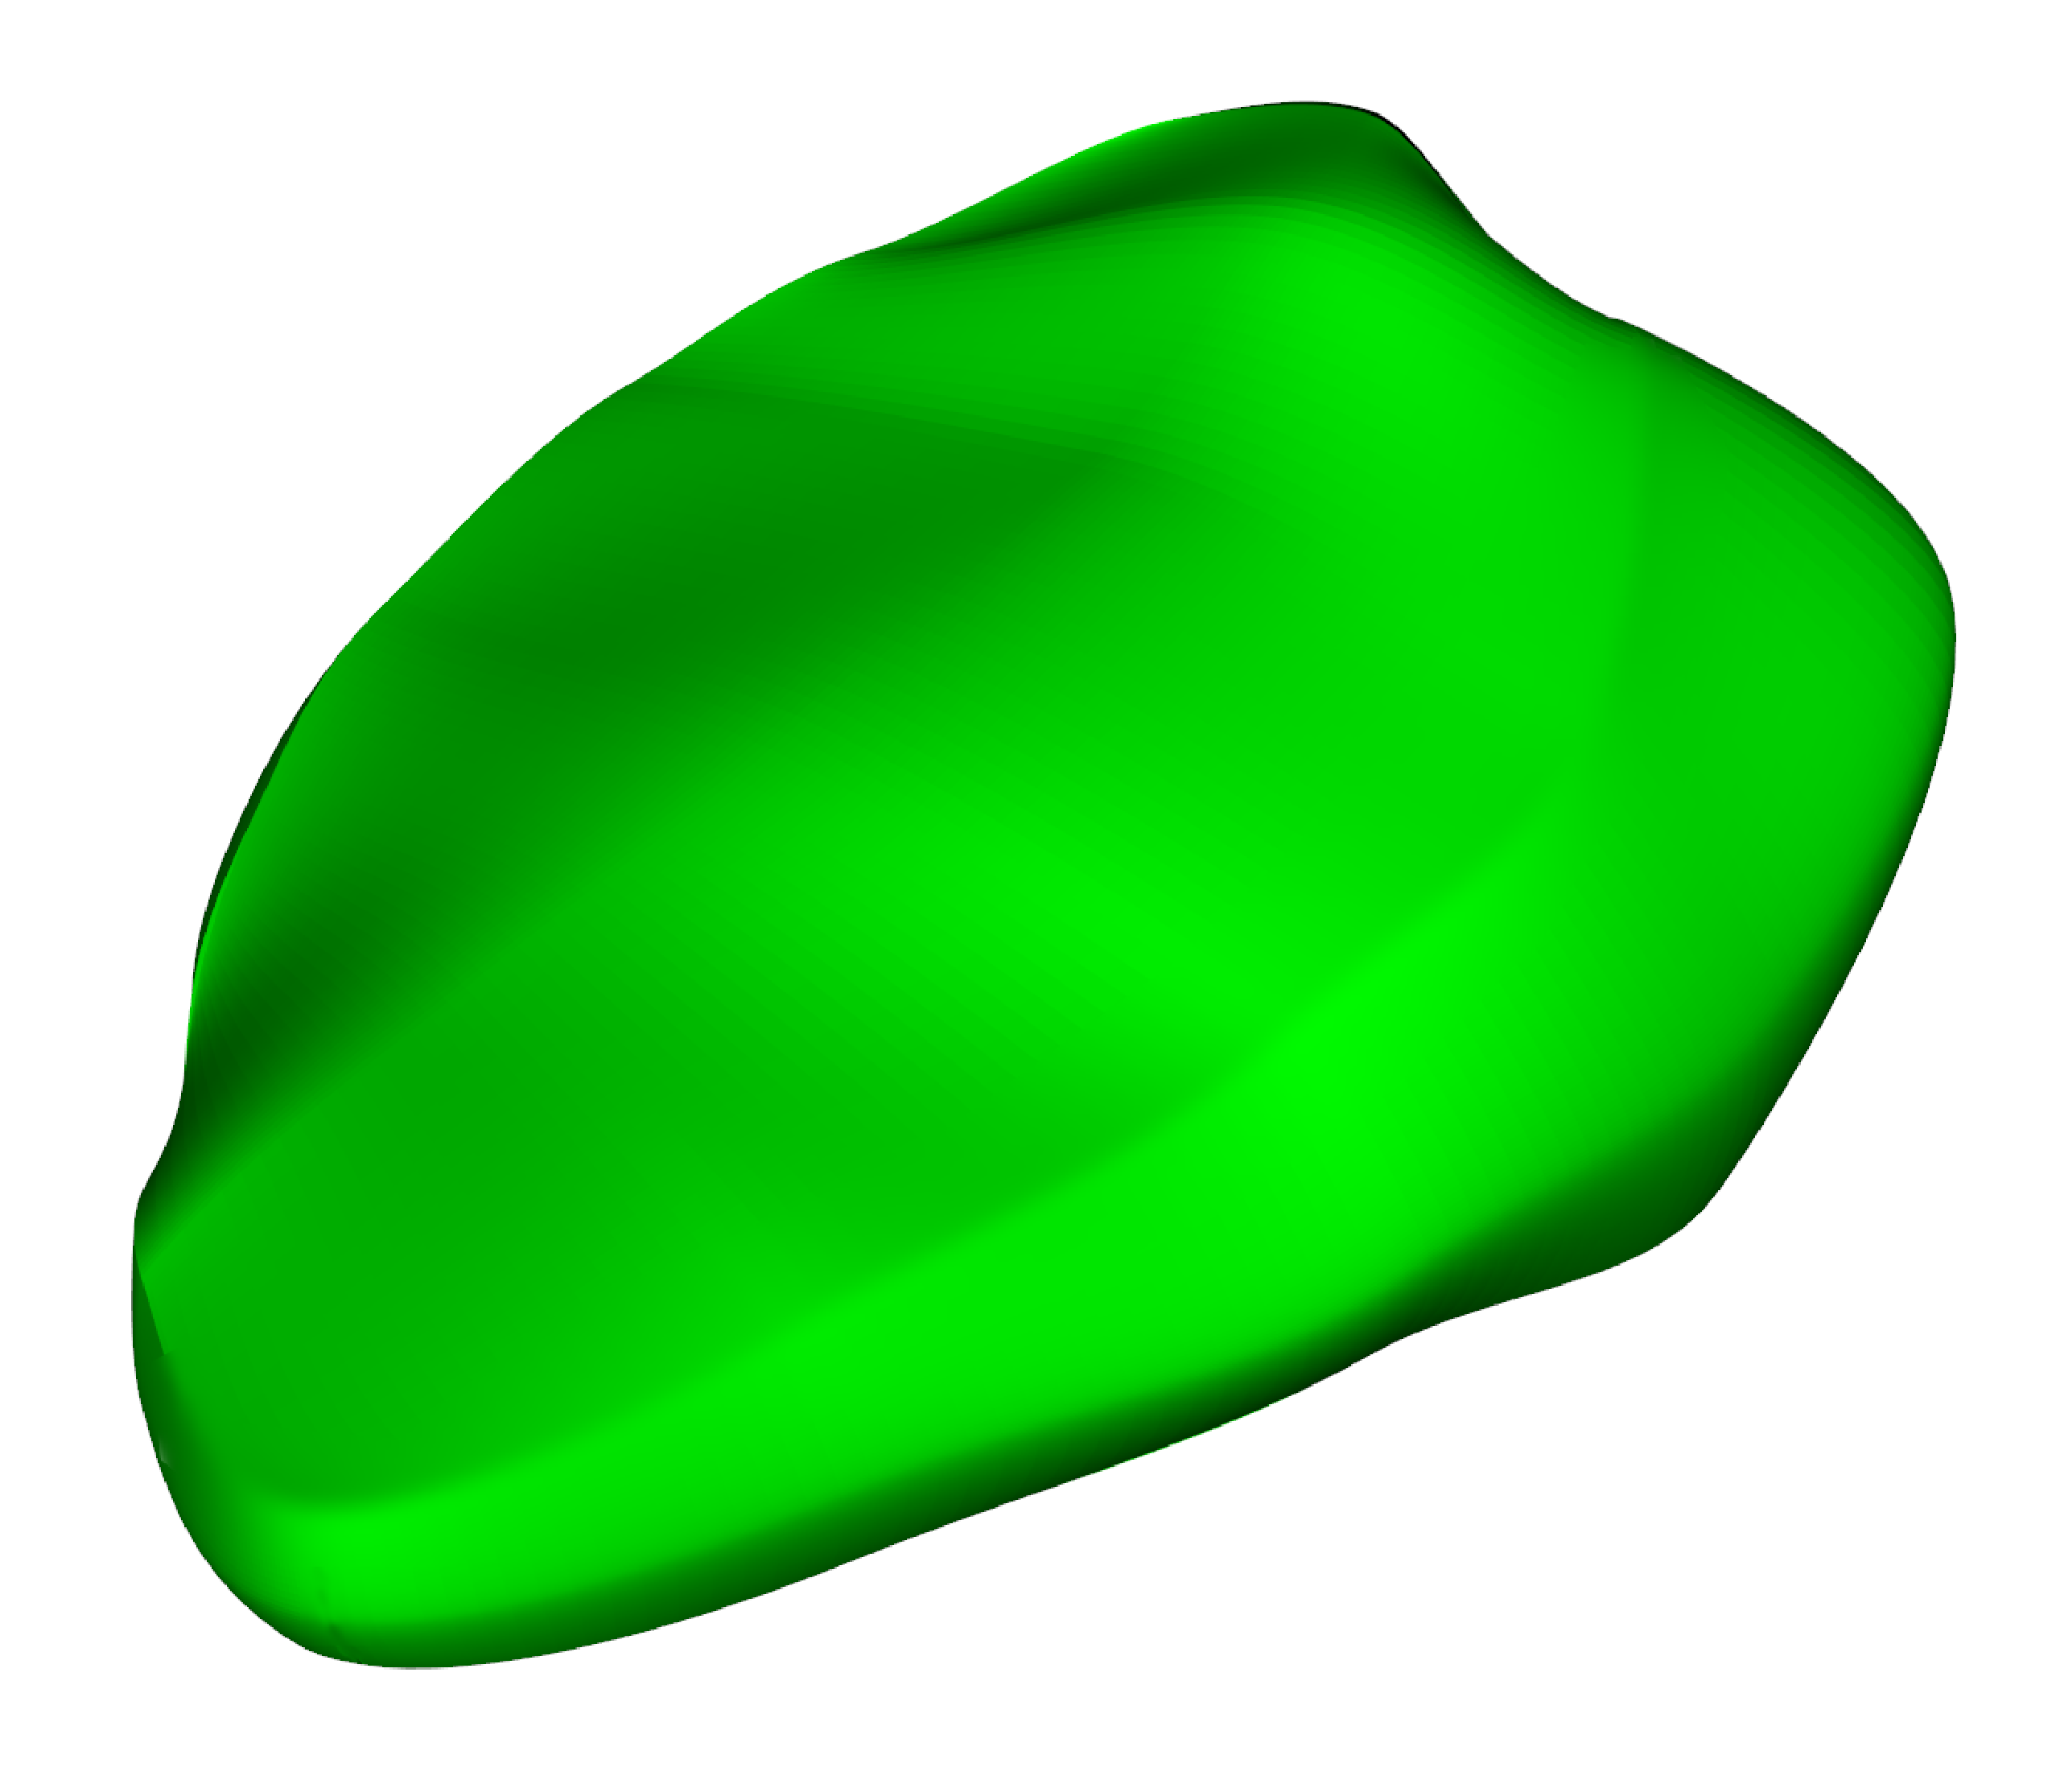
\epsfig{file = interpolationSrepSurface.eps, width = 8cm}
 \caption[Amygdala's s-rep.]{Complete s-rep of an amygdala, with top, bottom and crest surfaces. 
          The level of interpolation is higher to produce a smoother boundary.}
 \label{fig:srepInterpolated}  
\end{figure}

\subsubsection{Tubular objects} 

Different organs in the human body, 
such as blood vessels, the airways, and the intestines 
among many others are best represented using tubular structures.
Representing these objects with slab type s-reps is more difficult, 
because SS cannot be oriented in an intuitive manner. 
Instead, a parameterized space curve provides a more stable representation of a SS. 
Prominent authors such as \cite{binford1971visual}
proposed generalized cylinders, 
this method consists of a space curve, 
or axis, and a cross section function defined on the axis. For example, the function may be an ellipse. 
Another approach is the one proposed by \cite{huang1993generalized} named generalized tubes.
It is a two step approach, to segment and model tubular structures.
It starts with a local contour detection followed by a global 
recognition stage where the tube figures from the first stage are verified.
Such tube figures have been widely used on segmentation and modeling procedures,
but unfortunately, it is not trivial to include shape statistics using the approaches mentioned before;
such structures are best conceived to model individual tubes and not a population of them.
For this reason the tubular model proposed here is closely related 
to quasi-tubes, a model proposed by \cite{saboomedial}.

\begin{figure} 
 \centering  
  \subfigure[Interpolated spokes of a tube figure, the MA is shown in yellow and the spokes in cyan.
             The MA is parameterized by a single parameter $u$, while the spokes on the MA are parameterized by $(u, \phi)$, 
             $\tau$ represents the portion of the spoke from the MA to the boundary.]{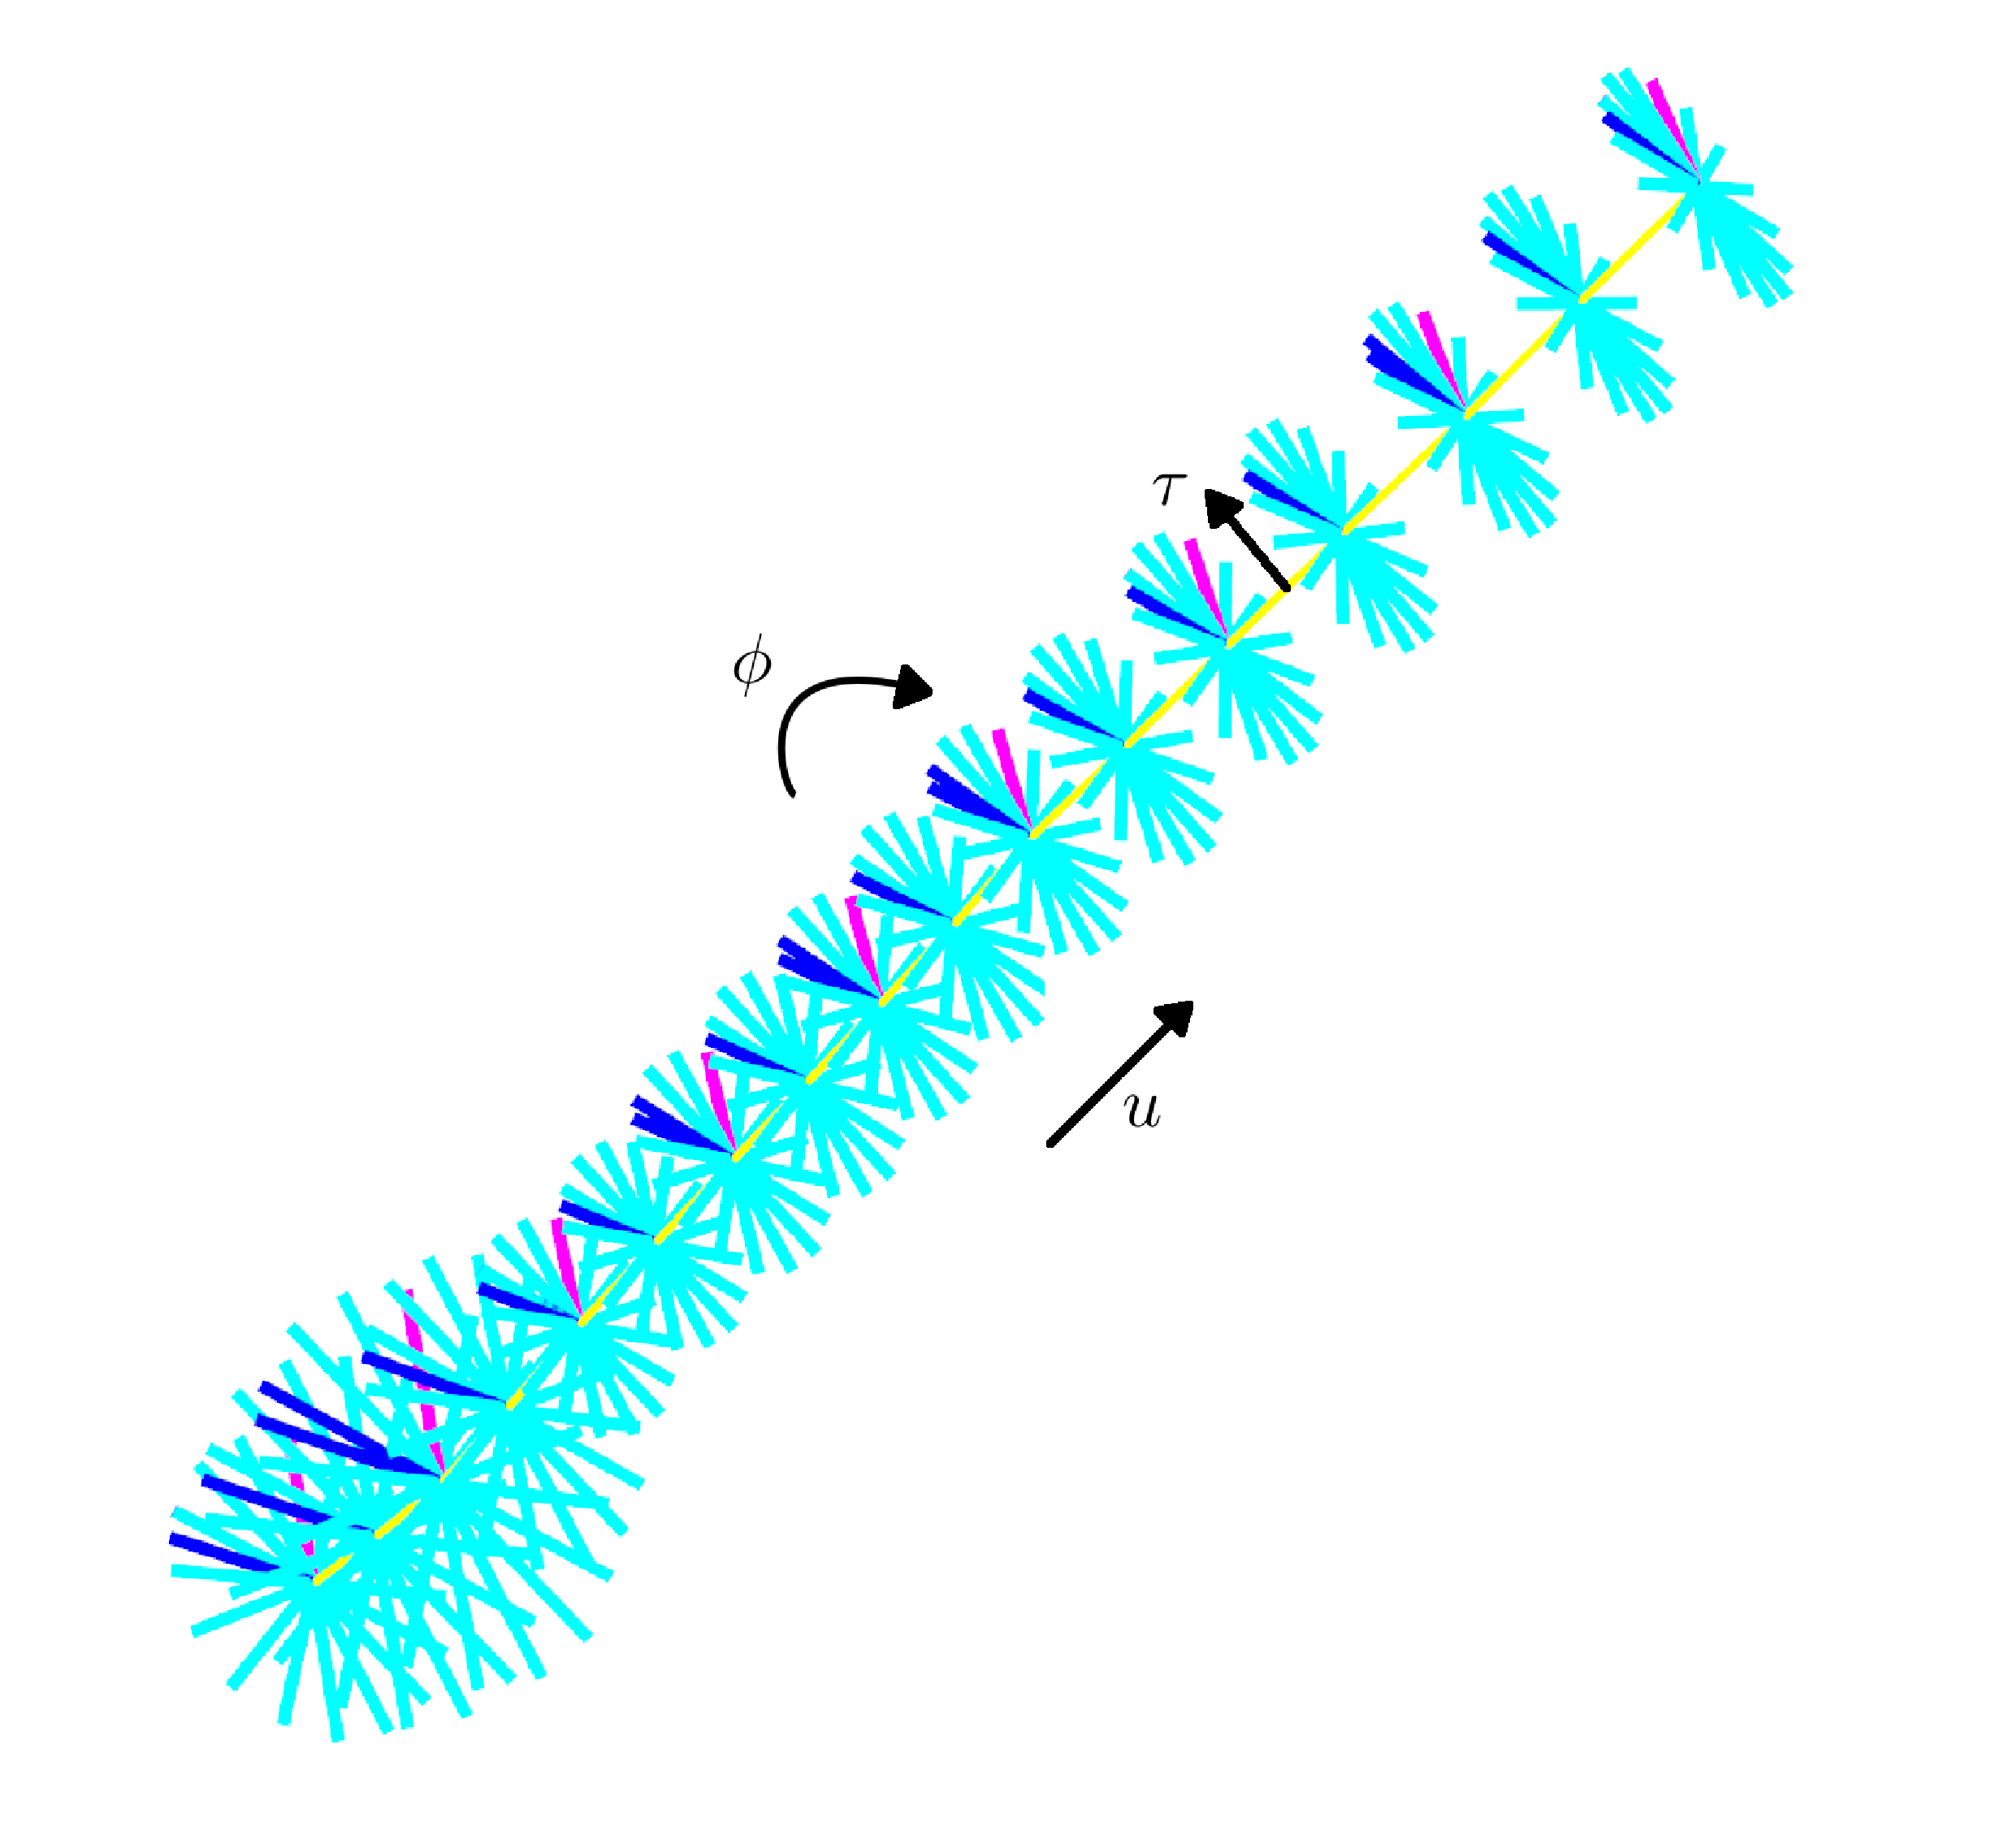
\epsfig{file = interpolationTube0.eps, width = 6cm}}
  \subfigure[The union of spoke tips produce the boundary of the tubular object]{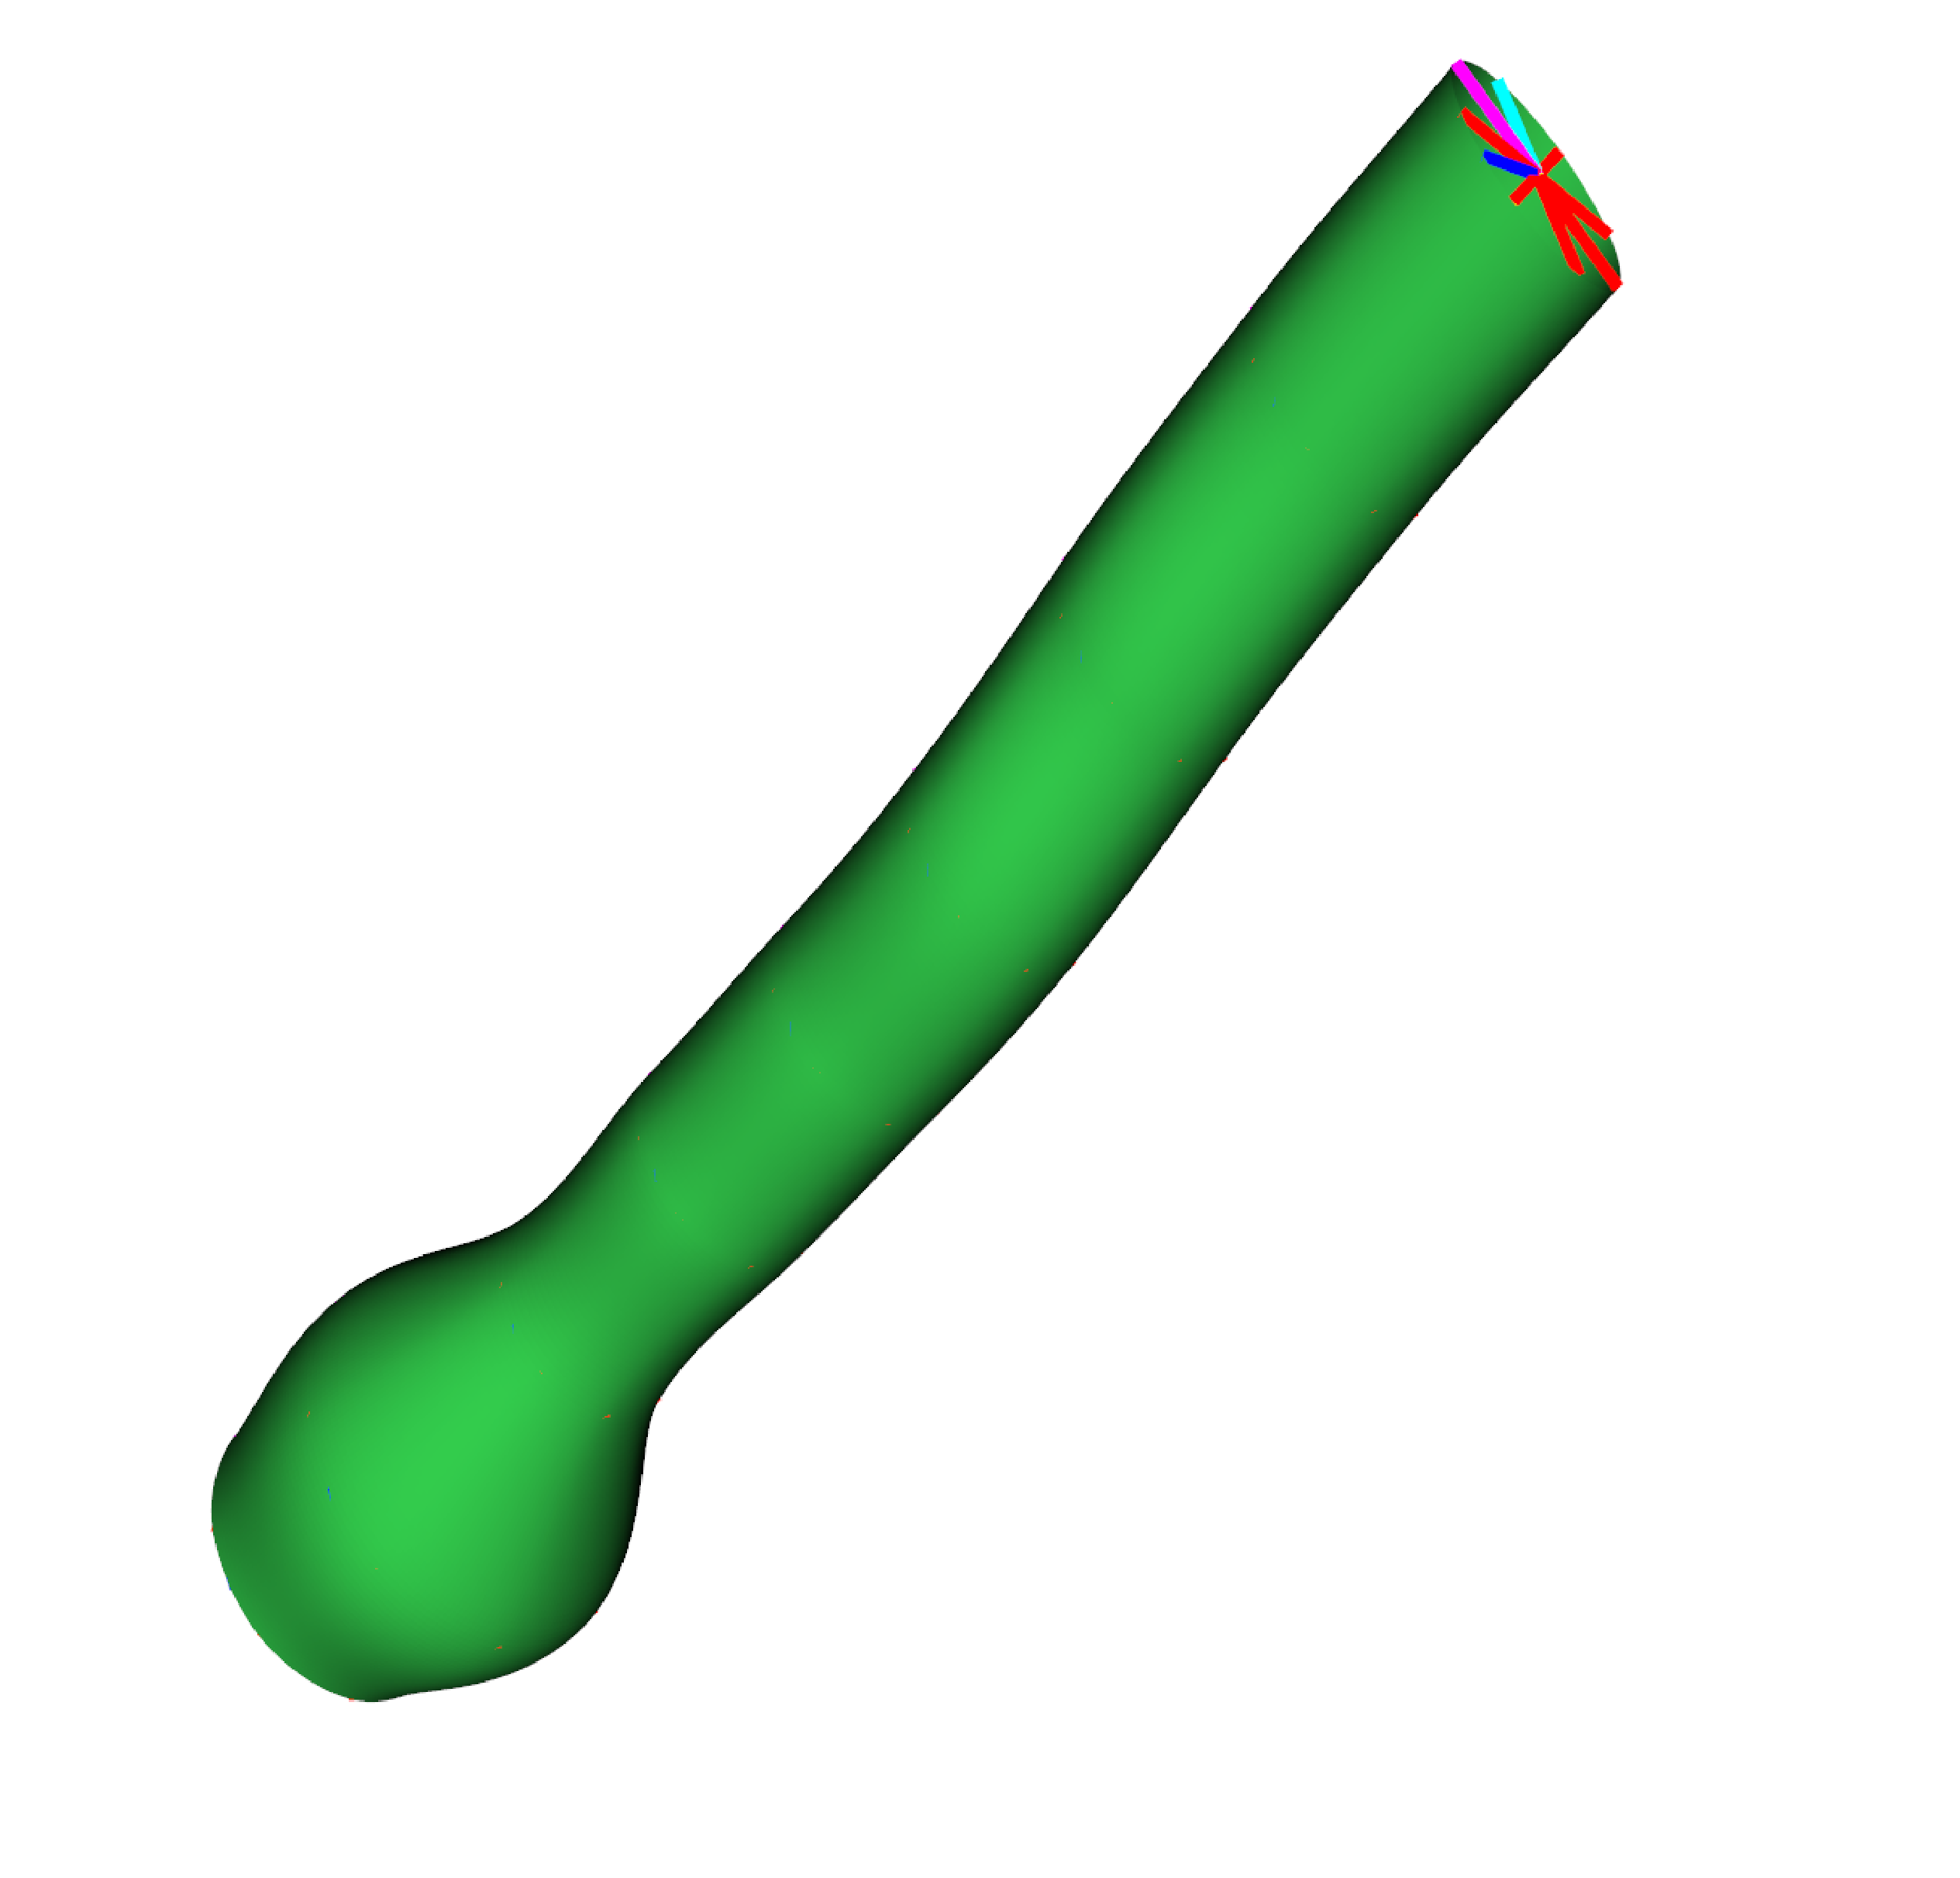
\epsfig{file = interpolationTube1.eps, width = 6cm}}
 \caption[Quasi-tube interpolation.]{The crest interpolation method is also capable of interpolating tube figures.}
 \label{fig:tubular}  
\end{figure} 

Figure  \ref{fig:tubular} shows the result of the interpolation using the same 
formulation from the crest method. 
These quasi-tubes are defined in the same manner as s-reps, $S_{rep} = \{p_i, S_i\}$; 
the difference is that the spokes are all placed following a space curve that 
defines the MA, and the interpolation is done with the spokes that share the same hub.
They are differentiated by the angle $\phi$ from 
the spoke located at $\phi = 0$ which is highlighted in magenta. 

Since the definition of this tubular object is equivalent to 
the definition of an s-rep, 
the statistical framework CPNS 
is also compatible. 
However, tubular objects are not widely used in this dissertation and
will be reserved for future work. 

The last subject that is addressed on geometric representation
is the internal coordinates of an object.

\subsection{Internal coordinates of an object}
\label{sec:internalCoordinates}

The internal coordinates of an object are described by $X2U$ maps. 
The mapping enables querying world coordinates to find object coordinates.
$X2U$ maps will be used in Chapter \ref{chapter:MRISimulation}
to map the solids generated in Chapter \ref{chapter:textureSynthesis} 
to an s-rep. This is possible since the solids are synthesized 
in a cube. Each coordinates in the cube can be related to $[u, v, \tau]$, thus, providing 
a simple mechanism to map a solid to an object. 

The amygdala shown in Figure \ref{fig:srepInterpolated} 
is composed by 18 atoms placed on a double sided grid $(m, n) = (6, 3)$, where every spoke's tail is placed.
The total number of spokes is 26 and
in order to give
a unique coordinate to every spoke, 
the MS is unfolded. 

\begin{figure} 
 \centering  
 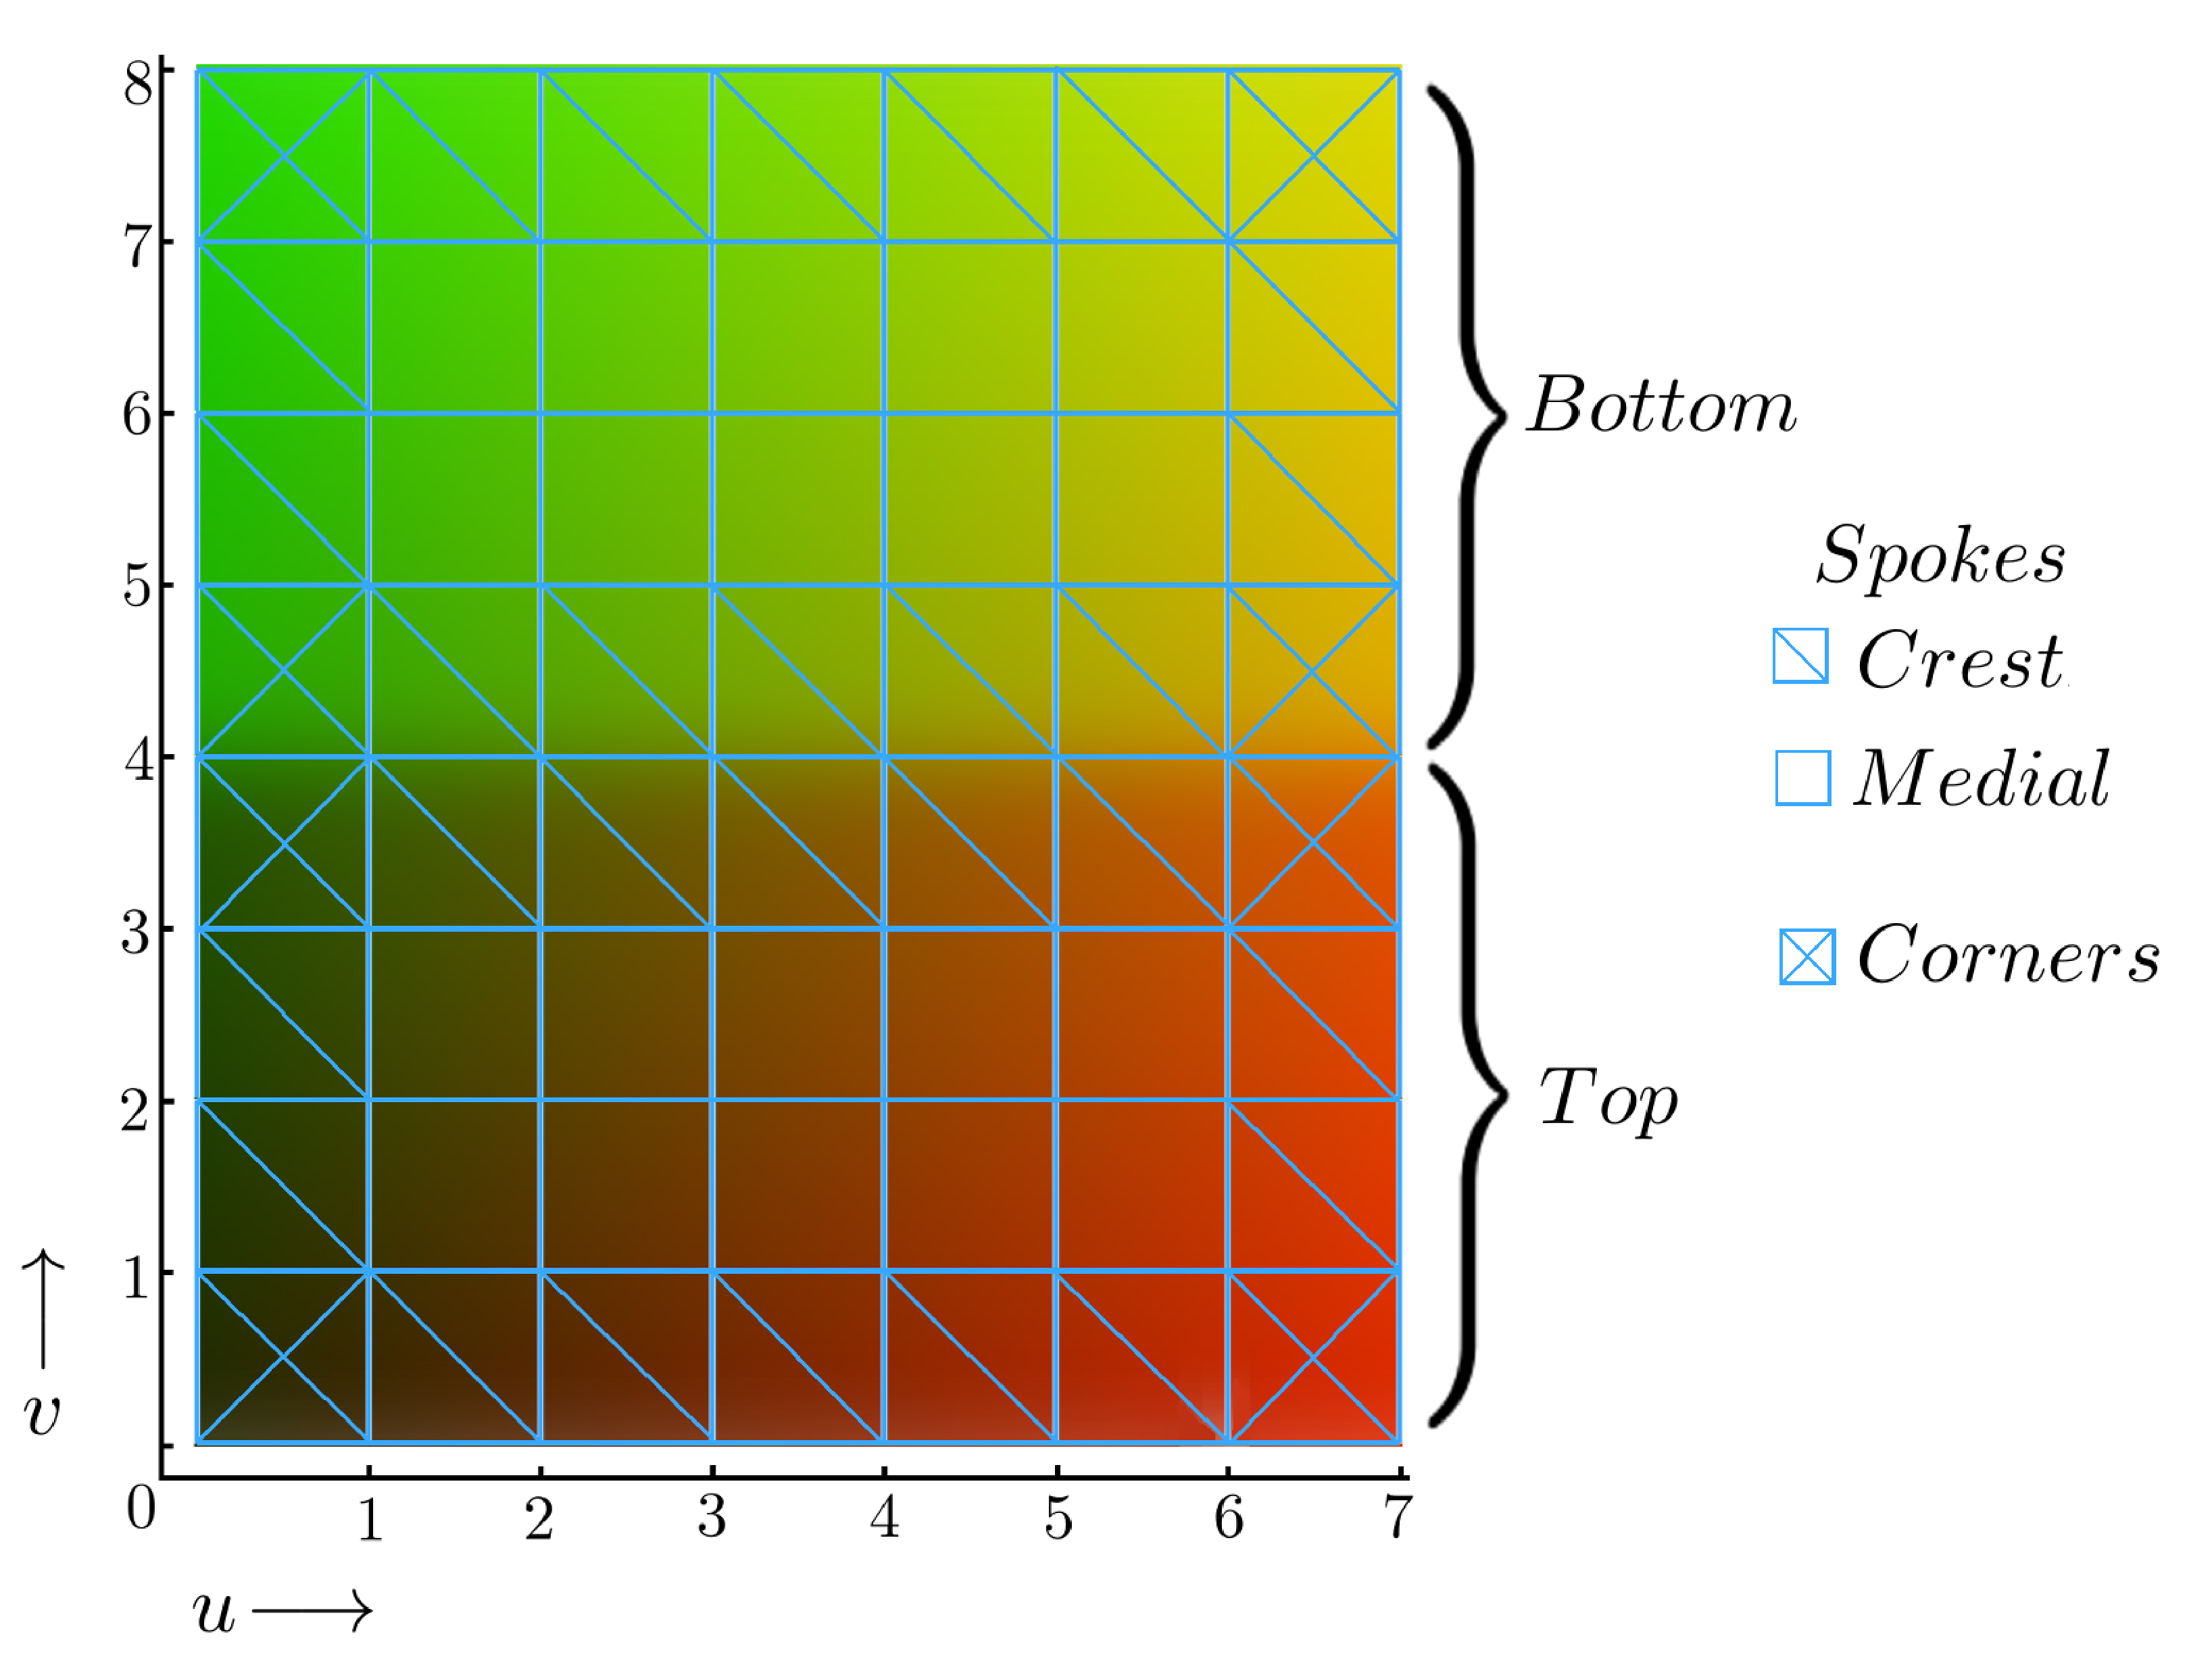
\epsfig{file = x2uMapGrid.eps, width = 13cm}
 \caption[Unfolding the s-rep.]{Unfolded s-rep of $6 \times 3$ atoms. Each intersection corresponds to a spoke in the s-rep,  
          the crest spokes repeat them selfs on the top and bottom sides. 
          The corners of the object are shown with the blue cross, 
          they also correspond to the 4 crest spokes that join top, bottom and connect the sides
          of the object. 
          Using this unfolded version of the MS we provide a unique $u, v$ value represented by the color gradient,
          the grid size is $(m + 1) \times 2\times(n + 1)$.
          }
 \label{fig:unfoldedSlab}  
\end{figure}

Figure \ref{fig:unfoldedSlab} shows a representation 
of the unique $(u, v$) coordinate given to 
every spoke in the object, they are represented by the color gradient
using red to for the $u$ direction and green for the $v$ direction. 
The blue color is used to represent the spoke length which is $\tau = 0$.

By means of the mechanisms described to interpolate the MS, top, bottom and crest spokes, 
a function $U2X(u, v, \tau) = [x, y, z] | (u, v, \tau) \in [0, 1])$ is designed to retrieve a position inside the 
object by querying $(u, v, \tau)$ coordinates.
This function is used to calculate the $X2U$ map. 

Figure \ref{fig:x2uMap} shows the $X2U$ map of the amygdala.

\begin{figure} 
 \centering  
  \subfigure[Top side]{
\epsfig{file = x2uMapTop.eps, width = 7cm}}
  \subfigure[Bottom side]{
\epsfig{file = x2uMapBottom.eps, width = 7cm}}
 \caption[X2U's map volume rendering.]{Volume rendering of an $X2U$ map showing both sides when $\tau = 1$}
 \label{fig:x2uMap}  
\end{figure} 


\section{Conclusions}
\label{sec:3dRepConclusion}

We have seen different types of approaches to model the boundaries of objects and produce statistics on 
their shape.
It has been shown that deformable models behave better 
and increase the accuracy of segmentation procedures or object recognition. They 
are less sensitive to noise and are more likely to find the global optimal object boundary.
Two major components in probabilistic deformable model methods are  
learning shape statistics and the segmentation of target images using the statistical probability distributions. 
There is still more improvement to be done 
at the training stage of the deformable model because this step requires 
too much user intervention and is time consuming. 

Besides surface modeling, a summary on 3D modeling techniques has been given. 
Those models are best suited to describe the internal features of 3D objects.
S-reps in particular are able to explain the continuum of space in an object, 
giving possibilities to include information into the model in a multi-scale fashion. 
The continuum of space described by the s-reps will be used  
to include the necessary parameters to perform MRI simulation. 

Furthermore, s-reps are suited to produce shape statistics with CPNS and can describe
shape variations with a few coefficients, a mean shape and eigenmodes of shape variation. 

The following chapter explains a novel methodology to 
fit s-reps to the brain cortex because they also support
foldability.
With the fitted structure a statistical analysis is conducted using CPNS
proving that s-reps are well suited to model 
complex structures. 

\newpage



\graphicspath{{ChapterCortex/images/}}
%% Chapitre I %%
\chapter{Cortex modeling via s-reps}
\label{chapter:cortexModeling}

\section{Introduction}
\label{sec:Introduction}

The cerebral cortex is a highly folded slab of neural tissue 
with compact interconnections that enables sophisticated processing of information.
It plays an important role in memory, attention, perceptual awareness, thought, language, and consciousness.
Progress has been made in understanding the structure and function of the cortex.
\cite{lorente1934studies} proposed that the cortex is formed by small cylinders containing vertical chains of neurons; 
These structures were later called columns, corresponding to groups of local cells running perpendicular to the cortical surface.
This hypothesis was later confirmed with the physiological studies done by \cite{mountcastle1998perceptual}. 

The cortex is a layered sheet with a more or less uniform cellular structure. 
It is composed by the following layers:
\begin{enumerate}
 \item Layer I (molecular layer): apical dendrites of cells and axons; 
 \item Layer II (external granular layer): small granule cells and some larger pyramidal cells;
 \item Layer III (external pyramidal layer): small to medium sized pyramidal neurons;
 \item Layer IV (Internal granular layer): interneurons receiving ascending sensory input and projecting to layers II/III. No pyramidal neurons are found in this layer;
 \item Layer V (Internal pyramidal layer): medium to very large pyramidal neurons; 
 \item Layer VI (Multiform layer): assortment of cell types including pyramidal cells, cells that receive input from layers II, III and V and 
       axons projecting to superficial cortical layers and subcortical regions.
\end{enumerate}
Today the columnar organization is the most widely adopted model to explain the cortical processing of information.

\begin{figure}[htb]
 \centering 
    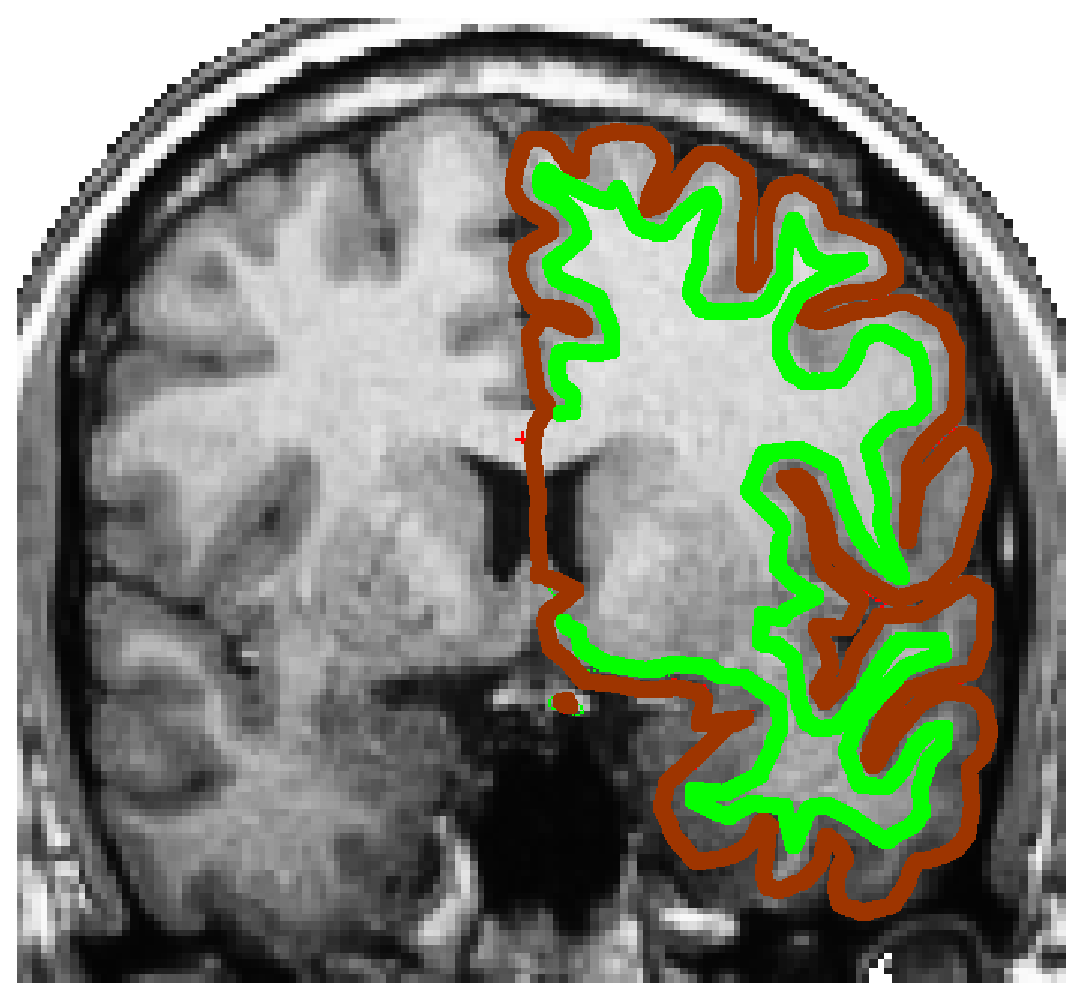
\epsfig{file = lh_BrainFreesurfer.eps, width = 8cm}
 \caption[Brain MRI.]{Brain MRI. The grey and white matter surfaces are shown in brown and green respectively.}
 \label{fig:MRIimage}  
\end{figure}

Figure \ref{fig:MRIimage} shows a slice of an MRI with the cortex region outlined. In brown the grey matter (GM) and in green the white matter (WM) surfaces are shown.
Since nearly two thirds of the cortical surface is buried within the sulci, it is difficult to perform computation and visualization tasks. 
Different procedures have been developed to unfold and map the cortical surface onto different spaces (inflated, spherical or flattened)
\cite{drury_computerized_1996}, \cite{hermosillo_unfolding_1999}, \cite{fischl_cortical_1999}, \cite{pons_area_2004}. 
This allows the cortical surface to be analyzed and visualized and statistical methods to be applied on these spaces.
\textit{Freesurfer} (an automated tool for brain's cortical surface reconstruction using structural MRI data)
uses the inflation and flattening procedure from \cite{fischl_cortical_1999}. 

Likewise, cortex evolution has also been a subject of great interest.
Much of the efforts have been focused on understanding how the folding process occurs.
Many species have folded cortices, but the degree of folding is different among them.
In general terms, a greater degree of folding is related to higher intelligence \cite{buettner1964evolutionary}.
Humans have extremely folded cortices.
%how this process occurs is not clearly understood. 
The folding patterns are 
unique to each brain, and abnormal folding is related to 
neurological disorders such as schizophrenia, epilepsy, autism and Down's syndrome.
Different methods have been proposed to explain how the folding occurs: 
growing a 2D curve in a closed space \cite{raghavan1997continuum}; 
growing 2D and 3D truss elements constrained by radially aligned fibers \cite{toro2005morphogenetic}; 
using spherical wavelets on close surfaces \cite{yu2007cortical}; 
using a FEM (finite element method) biomechanical model \cite{geng2009biomechanisms};
combining a mathematical model with biomechanical data \cite{bayly2013mechanical}.
For a recent review on folding theories see \cite{filas2013mechanisms}.

There are research opportunities in developing cortex models. 
As stated by Javier de Felipe \cite{defelipe2012neocortical}, ``it is still necessary
to achieve a better fundamental understanding of what columns
are and how they are used in cortical processes. Accordingly, it
is now important to translate recent technical advances and
new findings in the neurosciences into practical applications for
neuroscientists, clinicians, and for those interested in comparative
anatomy and brain evolution.''

Taking these facts into consideration, one of the objectives in this dissertation is to provide a
tool that models the shape of the cortex and relates to the real physical structure. 
Section \ref{sec:s-repImplementation} defines an s-rep
with the corresponding interpolation mechanisms that parameterize the interior of the object by $[u, v, \tau]$.
S-reps can be used to model the anatomic and physiologic information from the different layers of the cortex.
This information can be naturally included using the $\tau$ coordinate.

\begin{figure} 
 \centering 
	\subfigure[]{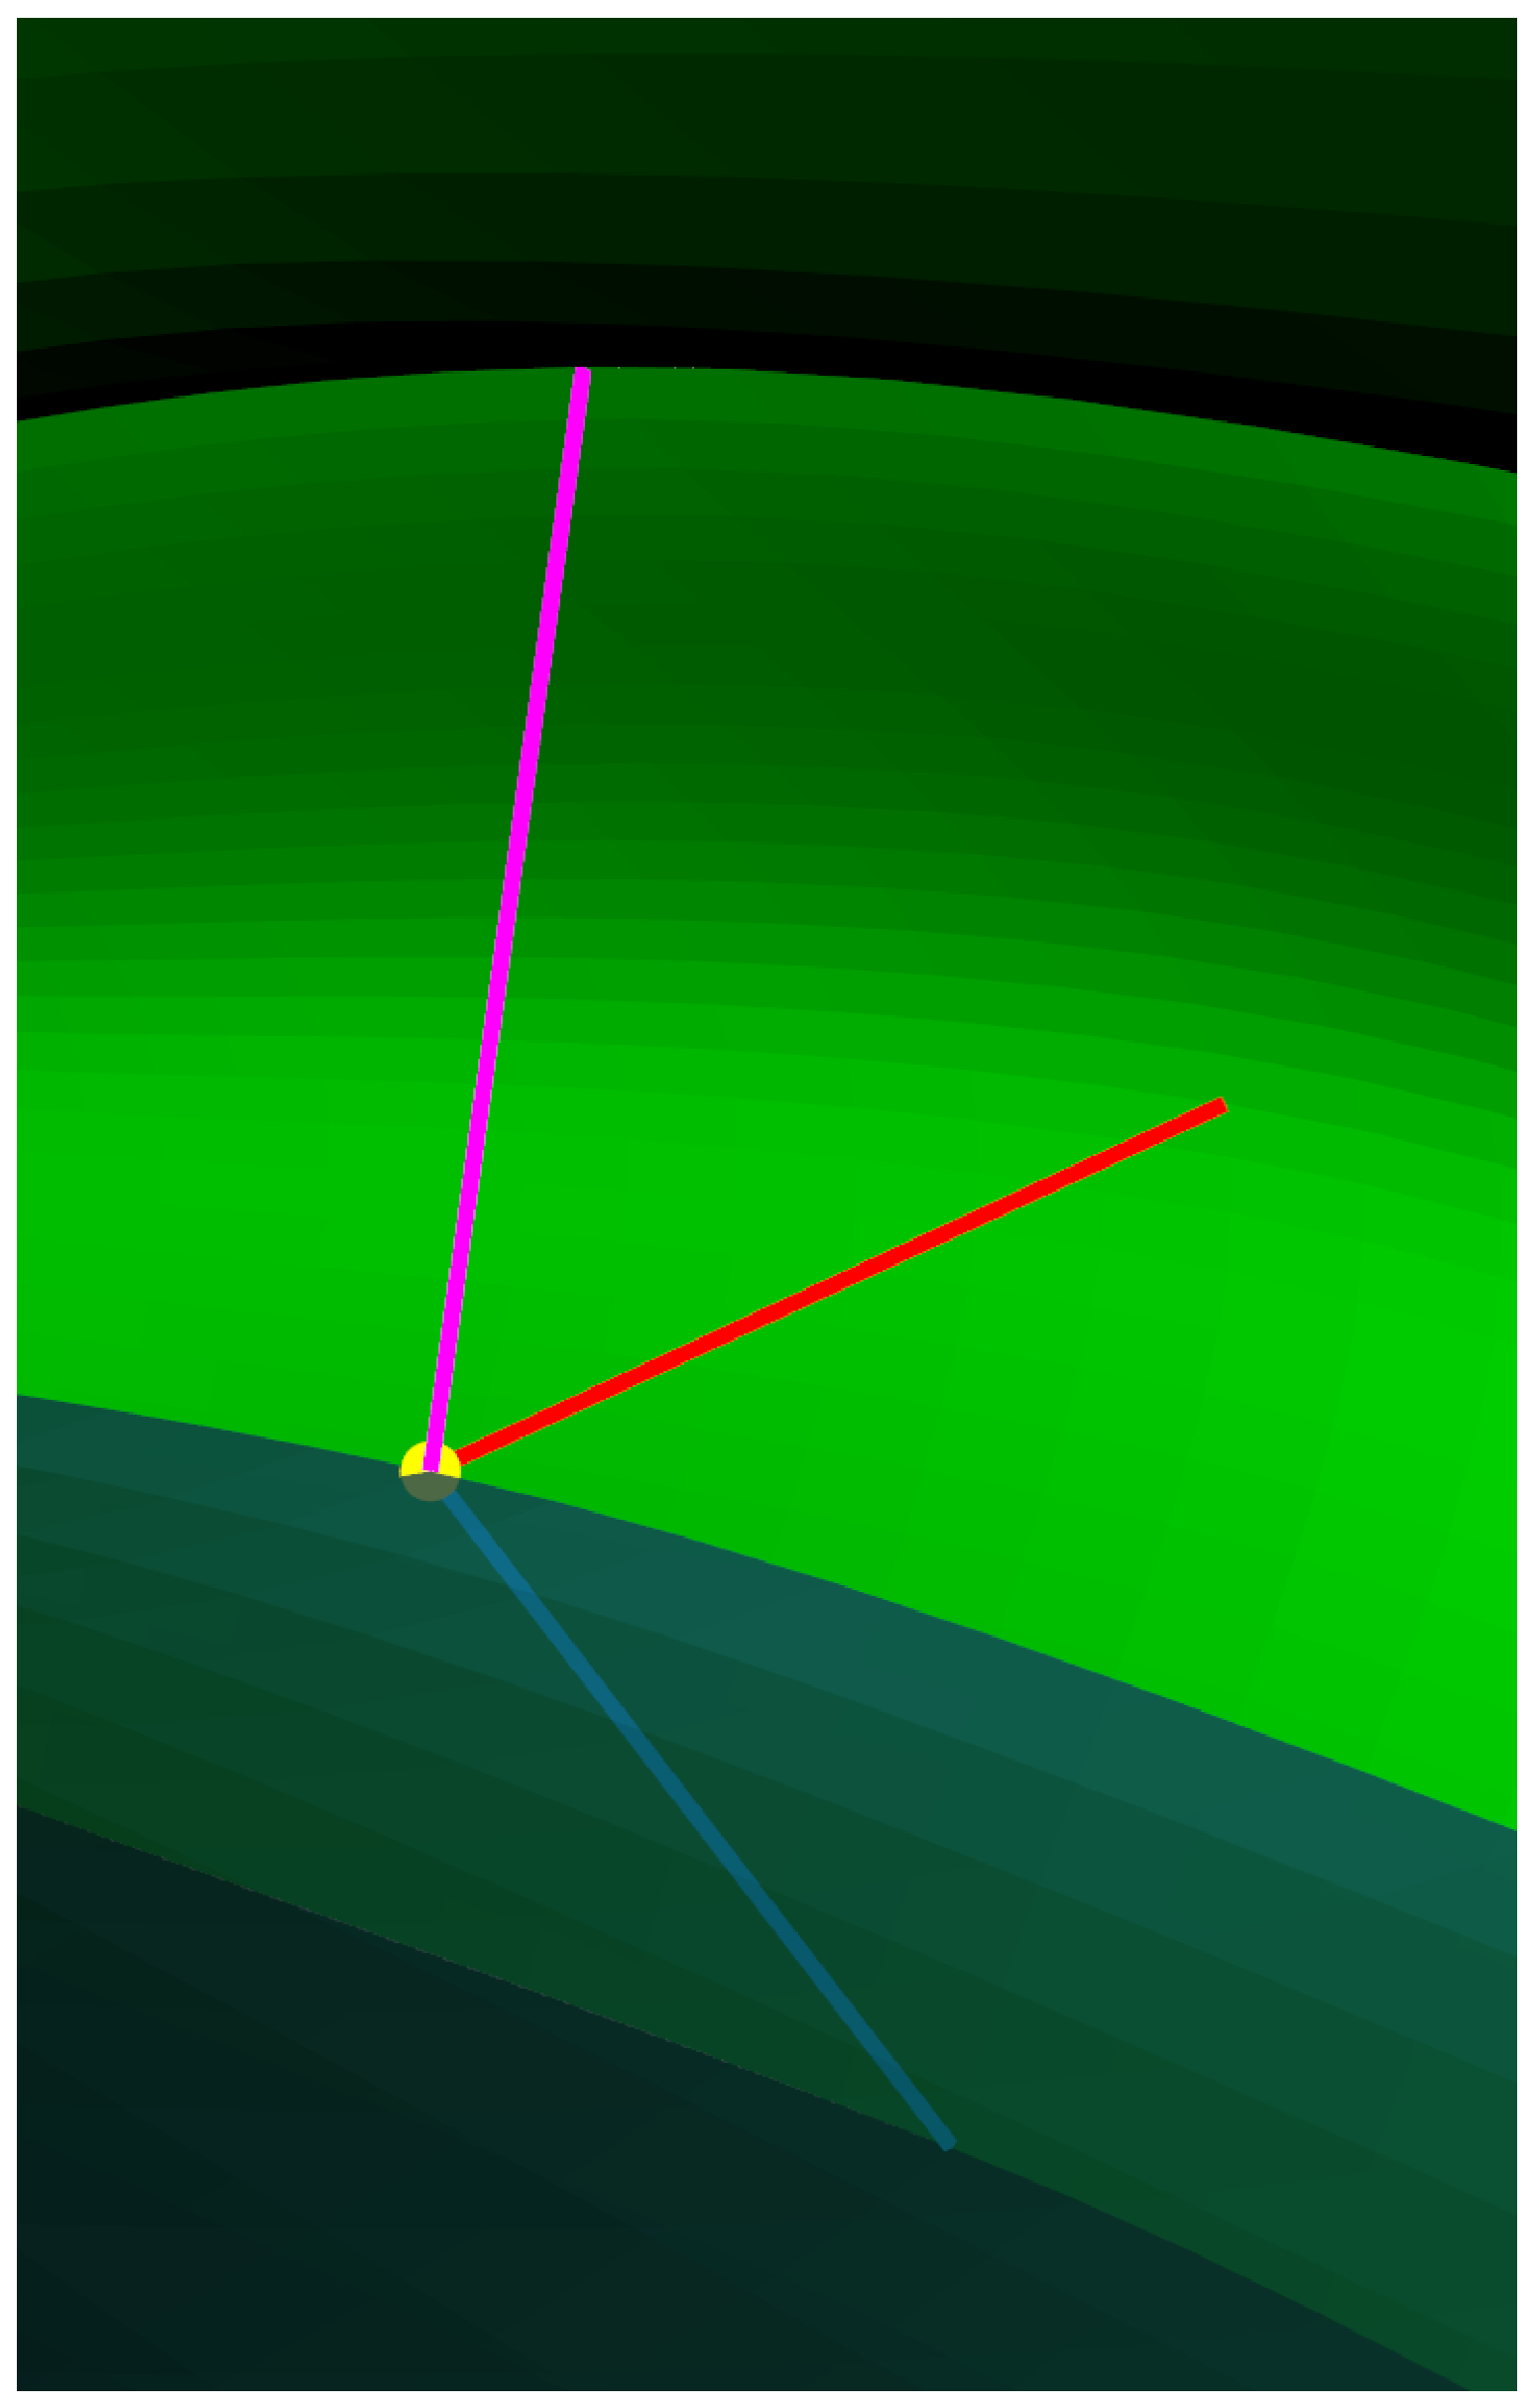
\epsfig{file = s-repatomCloseUp.eps, width = 3.25cm}}
	\subfigure[]{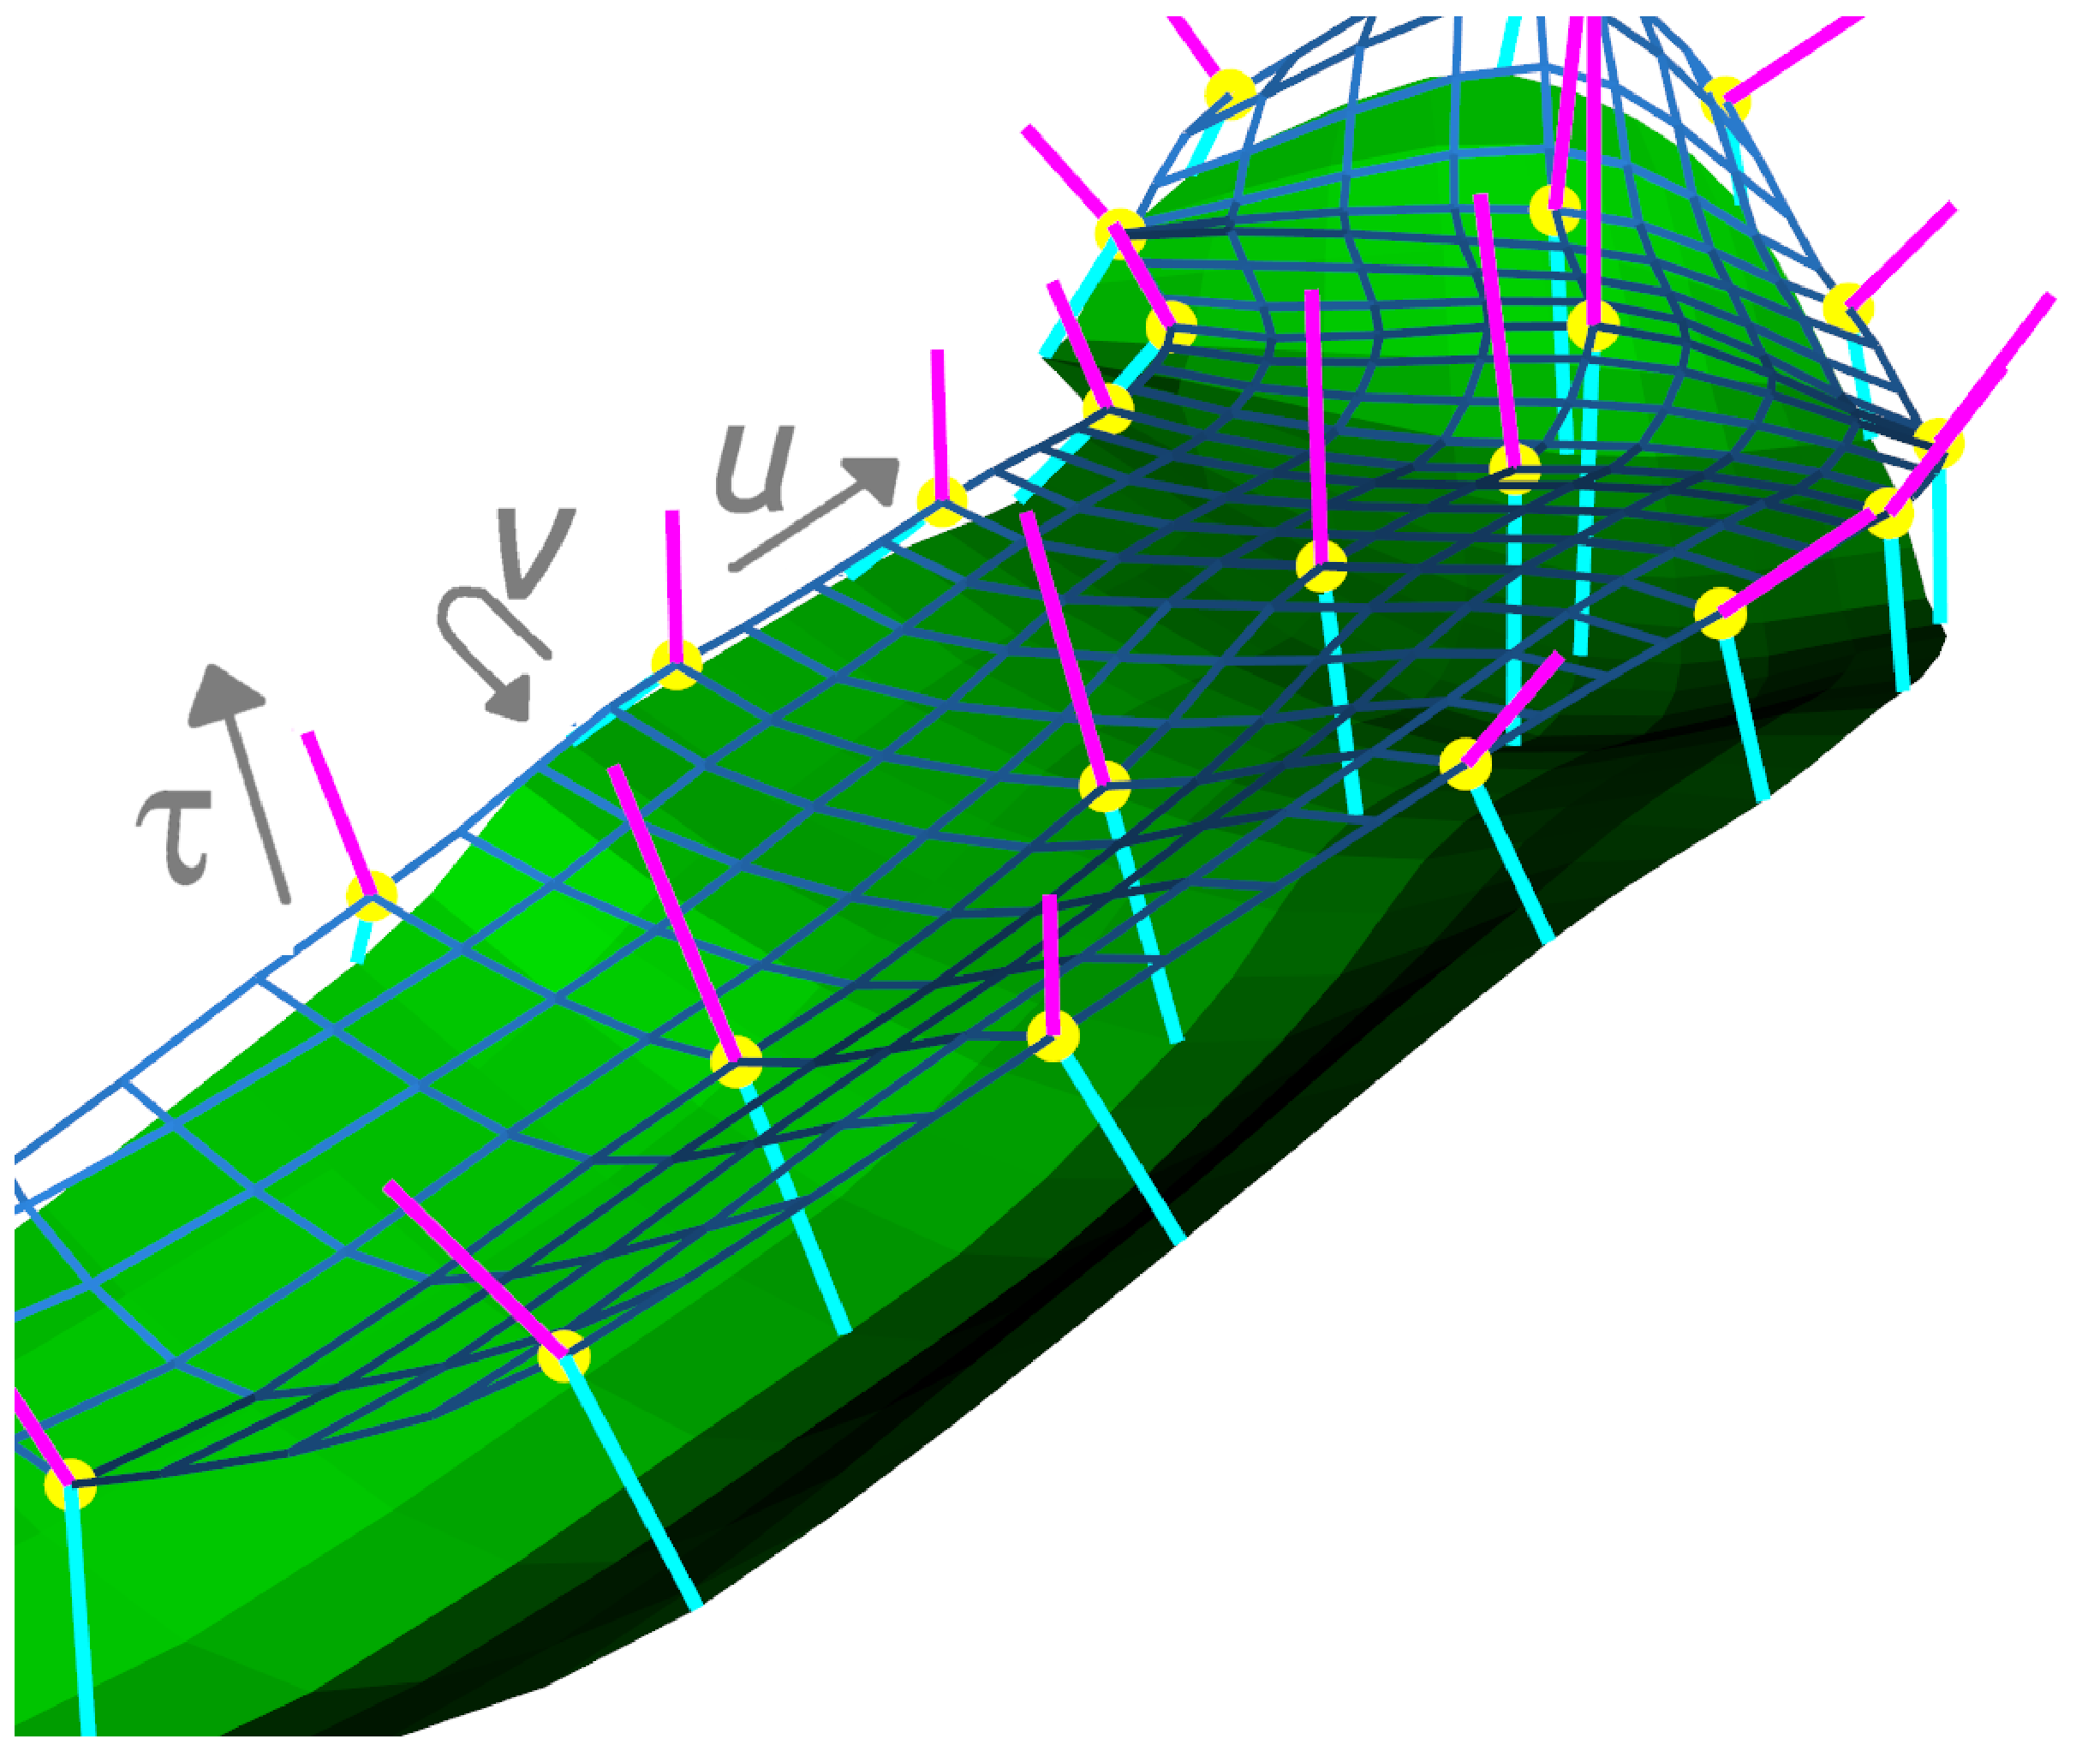
\epsfig{file = s-repFig.eps, width = 6cm}}
	\subfigure[]{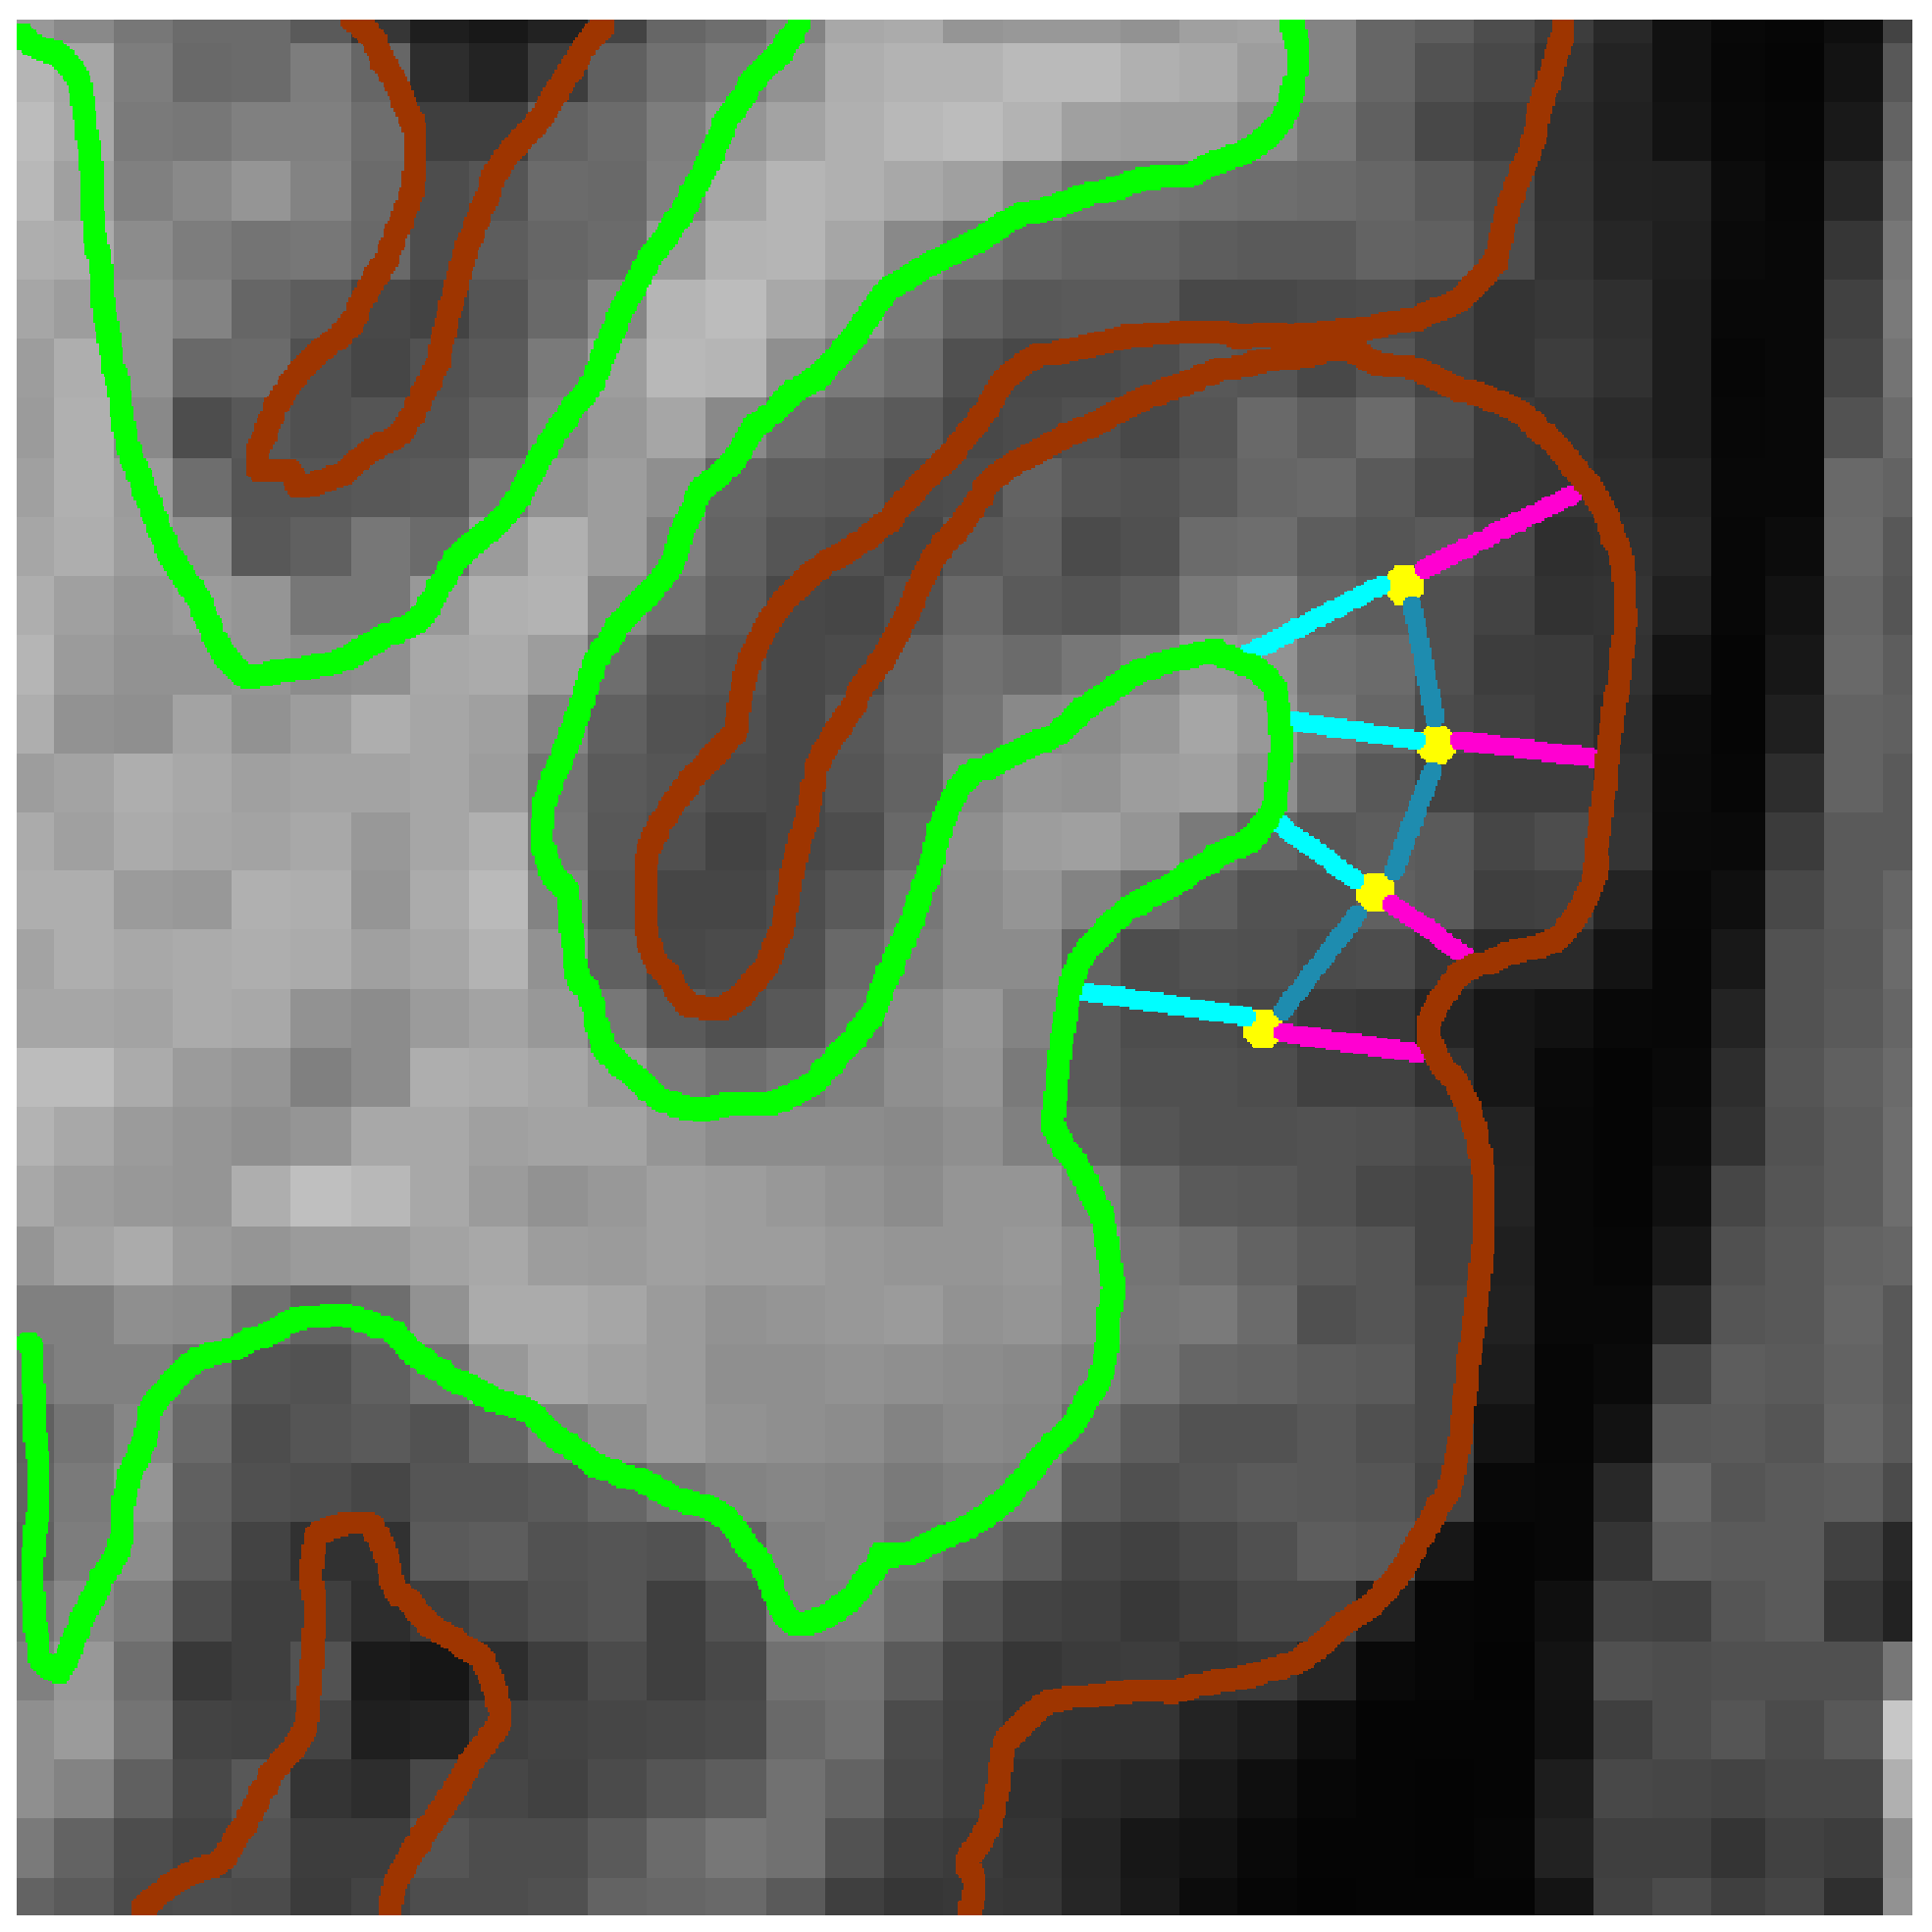
\epsfig{file = lh_BrainFreesurferZoom.eps, width = 5cm}}
 \caption[Atom close up.]{Figure (a) shows a close up of an atom represented as the yellow ball with its corresponding spokes, top (magenta), bottom (cyan), crest (red). 
          The s-rep on figure (b) shows the quasi-medial surface in wireframe representation (blue), with the sampled atoms.
          The MRI image on figure (c) shows a cross-section of the skeletal locus of the cortex and some atoms with the corresponding top and bottom spokes.}
 \label{fig:srepfigCortex}  
\end{figure}

%S-reps are defined as continuous objects using the interpolation mechanisms described in \cite{pizer_nested_2012},
%meaning that every point inside the object has a unique set of coordinates $[u, v, \tau]$. $u$ codes the width, $v$ the length of the medial locus,
%and $\tau$ the thickness of the object.
%$u$ varies from 0 to 1, $v$ wraps around the object with $v < 0.5$ on the ``anterior'' and $v > 0.5$ on the ``posterior'', and $\tau$ 
%from the skeletal locus to the object boundary, as shown in Figure \ref{fig:Srepfig}-b.
%The union of vectors form the object boundary and the union of tails represent the ``skeletal locus''. 
%Notice that s-reps model the continuum space, opening the possibility to include the cellular level and describe the layered structure 
%of the cortex.
Figure \ref{fig:srepfigCortex} shows how an s-rep fits into the cortex. 
%From now on the word s-rep is used to reference the discrete version of the object.

Besides shape description, s-reps have been used successfully to compute shape statistics and mean shapes from a population 
of objects. 
%This is done using CPNS a method analogous to PCA \cite{pizer_nested_2012}.
With this statistical description, it appears to be possible to classify objects by shape frequently more accurately than any other method.
%The majority only use surface information; in contrast, the skeletal structure brings 
%stability to the statistics and increases the correspondence of information across the population of objects.
%S-reps have been used to model internal brain structures such as the hippocampus \cite{pizer_nested_2012}. 
S-reps model single non-branching objects, and tubular objects, as explained in Section \ref{sec:quasiMedial}.
The objects modeled with s-reps until now are simple as most of them have a 
blob-like or elongated shape structure like the the hippocampus \cite{pizer_nested_2012}.

It is demonstrated that s-reps are suited to represent a folded complex structure such as the cortex.
The sheet of the object does not branch and captures the majority of the folds in the cortex. 
Moreover, a statistical analysis of shape variability is done using the s-rep description of the cortex.

The following section explains how to create an s-rep of the cortex from an MRI image.
The procedure uses a spherical representation of the cortex  \cite{fischl_cortical_1999} 
that relates the WM and the GM surfaces to the sphere.
Folding the s-rep into the cortex is done by 
projecting the SS (skeletal sheet) of the s-rep on the sphere and 
using the relationship of the sphere and the cortical surfaces.
%The folding procedure uses a function 
%that minimizes the distance to a set of closest points in the WM and GM surfaces.
%The procedure is done for every atom. It maintains
%the topology and regularity of the quads 
%or quadrangles that form the SS of the s-rep (quad definition in Equation \ref{equ:Quad}).
The following section explains in detail the procedure to create an s-rep of the cortex.
With the skeletal figure inside the cortex, 
top and bottom spokes point towards the GM and WM surfaces respectively.
The interpolation mechanisms of the s-rep allows reconstructing the GM surface and the WM surface.
Section \ref{sec:Evaluation} evaluates the quality of the interpolated surfaces.
Finally, a population of cortex s-reps is generated, and a statistical analysis is made in Section \ref{sec:Statistics} using CPNS (Composite Principal Nested Spheres, which is  
described in Appendix \ref{sec:apendixCPNS}).

\section{Acknowledging the true shape of the cortex}
\label{sec:s-repFittingCortex}


\begin{figure*} 
 \centering 
	\epsfig{file = DiagramProy.eps, width = 15cm}
 \caption[Flow diagram of s-rep projection and cortex folding.]{(a) Inflation of the cortex by \textit{Freesurfer} and rotation of the sphere to the north using the points in the corpus callosum. 
          (b) Transformation of a base s-rep into a circle.
          (c) Transformation of the circle into a sphere. 
          (d) Fitting the s-rep to \textit{Freesurfer's} data on the sphere.
          (e) Folding the SS of the s-rep inside the the cortex and determine the widths of the slab. 
          }
 \label{fig:proyProcedure}  
\end{figure*}

The cortex is a highly folded sheet. It has thickness that varies through the cortical regions. 
Unfortunately, the cortex is often represented using surfaces and is difficult to 
represent interior  features.
To acknowledge its true shape which is similar to a folded pancake, 
a procedure to create an s-rep of the cortex is proposed. 
As shown in Figure \ref{fig:proyProcedure}, the procedure has five steps:

\begin{enumerate}[(a)]
 \item A mapping of the cortex on a sphere is done using the method from \cite{fischl_cortical_1999}. 
       The sphere is rotated to the north using the corpus callosum.
 \item A regular grid or the SS of a base s-rep is transformed into a 'circular log-grid'.
 \item The 'circular log-grid' is transformed into a sphere (with a spherical cap oppening in the north pole).
 \item The SS on the sphere is fitted to the mapping of the cortex on the sphere.
 \item The SS is folded back into the shape of the cortex. During the folding procedure, the widths of the slab or the thickness of the s-rep is determined.        
\end{enumerate}

The following sections explain the details of each step and shows how to create an s-rep 
of the cortex.


\subsection{Spherical representation of the cortex by \textit{Freesurfer} and rotation}
\label{sec:Materials}

The materials used in this study are 8 
MRI scans acquired at ``CERMEP - Imagerie du vivant'' 
%********************* 
on a Siemens 
Sonata system with a 1.5 T magnet, with gradients of 40 mT/m and an 8-channel head coil. 
The overall protocol includes anatomical acquisitions, spectroscopy and diffusion.

In this study, only T1-weighted anatomical images are considered. The 8 datasets were obtained by
the acquisition of millimetric sagittal slices from a 3D T1-weighted MPR sequence (repetition time (TR) = 1880 ms, echo time (TE)
Ms = 4).
The total acquisition time of each of these anatomical images was done in 18 minutes.

All the datasets were segmented using \textit{Freesurfer}.
%and the inflation and flattening procedure from \cite{fischl_cortical_1999}.
The method proposed by \cite{fischl_cortical_1999} 
creates a spherical representation of the cortex. It removes the folds from the surface using an energy functional 
with a distance term for unfolded or positive regions. 
An unfolded region is recognized by calculating the normal direction and the ordered cross-product
of the triangle legs for every face in the surface tessellation. If the resulting vector 
is anti-parallel to the normal direction, a negative area is assigned. 
The folds from the surface are eliminated when the area is constrained to be
positive everywhere.
After the inflation procedure, the cortical surface has spherical topology. 
A mapping of the cortex is made onto a sphere providing 
a $1-1$ relationship for every point on the cortical surface and spherical mapping.
%The spherical mapping is the key to construct the s-rep of the cortex. 

The procedure to build the s-rep of the cortex uses a modified stereographic projection.
The stereographic projection \cite{snyder_map_1987} was probably known to the Egyptians in its polar form, 
but Hipparchus (2nd Century B.C) was apparently the first Greek to use it, so he is considered its inventor. 
Ptolemy referred to it as ``Planisphaerum'', the name stereographic was given by Fran\c{c}ois d'Aiguillon in 1613.
The stereographic projection enables a mapping of the points on a plane
to the sphere and it has two properties that should be treated carefully:
%is conformal (preserves angles), azimuthal (all points are proportionally correct distances from the center point),
the scale increases away from the center of the projection,
and the point opposite to the center of the projection cannot be plotted (north pole).

The first step to do a stereographic projection is to choose the north pole. 
The north pole of the sphere cannot be mapped by the stereographic projection because it
maps to infinity. For this reason, the representation must have a spherical cap opening in the north pole.

The corpus callosum is a brain structure located 
beneath the cortex. It facilitates inter-hemispheric communication with a bundle of 200-250 million fibers for this task.
Figure \ref{fig:Corpuscallosum} displays the corpus callosum. 
This brain structure is used to find the north pole.
The points in the corpus callosum are used in a fitting procedure that minimizes the geodesic distance from each point to a circle. 
The center of the best fitting circle is chosen to be the north pole.
%The point opposite to the north pole is the center of projection.

\begin{figure} 
 \centering 
 \subfigure[The internal part of the left hemisphere of the cortex. 
            The corpus callosum is shown in the figure.
            The points that compose the corpus callosum are used in the minimization procedure.]{\epsfig{file = corpuscallosum.eps, width = 7.25cm}}
 \subfigure[Spherical representation of the left hemisphere. 
            The best fitting circle is shown in cyan and the projected points  
            on top of the circle in magenta. The center of the circle is aligned with the north pole.]{\epsfig{file = sphereRotationNorth.eps, width = 7.25cm}}
 \caption[Inflation procedure, mapping the cortex on a sphere.]{The inflation procedure maps the cortical surface onto a sphere. 
          The best fitting circle is found using the points of the corpus callosum.}
 \label{fig:Corpuscallosum}  
\end{figure}

To find the best circle for a set of points in a sphere, a method similar to \cite{jung_analysis_2012} is used.
A circle on the sphere $S^2$ is defined by a vector $v_1$ and a distance $r_1 \in (0, \pi/2]$ as in equation \ref{equ:circle0},
where $\rho_d$ is the geodesic distance function.

\begin{equation}  
	C(v_1, r_1) = \{x \in S^2 : \rho_d(v_1, x) = r_1\}.
  \label{equ:circle0}
\end{equation}
The best fitting circle is found with a least squares minimization
that uses the geodesic distance as follows:
let $CC = \{x_i: i \in N\} \in S^2$ be the points of the corpus callosum on the sphere. We first define the residual $\varepsilon$ of $x_i$ from a circle
$C( v_1 , r_1 )$ of $S^2$ as the signed length of the minimal geodesic that joins $x_i$ to $C$. Then 
$\varepsilon = \rho_d( v_1 , x ) - r_1$. The sign of $\varepsilon$ is negative if $x_i$ is in the interior of $C$, and is positive if $x_i$ is in the exterior.
The best fitting circle $\hat{C} \equiv C( \hat{v}_1 , \hat{r}_1 )$ 
is found by minimizing the sum of squares of residuals of the data points to $C$. 
In other words $v_1$ and $r_1$ minimize Equation \ref{equ:optimalcircle}.

\begin{equation}  
  \hat{C} = \operatorname*{Arg\,min}_{v_1, r_1} \sum_{i=1}^{n} \varepsilon_i ( v_1 , r_1 )^2 = \operatorname*{Arg\,min}_{v_1, r_1} \sum_{i=1}^{n}\{\rho_d(x_i, v_1) - r_1 \}^2
  \label{equ:optimalcircle}
\end{equation}

Once the center of the circle is found, 
a rotation is done to align its center to the north pole. 
%A second rotation is performed to align it with the x axis. 
%This is done by finding the average point on the circle for the projected data, calculating the tangent at this point,
%and computing the opening angle with the x axis.
Figure \ref{fig:Corpuscallosum} shows the corpus callosum and a spherical representation 
of the cortex with the best fitting circle. 

The following section explains how to modify the s-rep 
to produce the best possible mapping on the sphere. 
The projection to the sphere is explained in Section \ref{sec:StereographicProjection}.

\subsection{Transforming the s-rep into a circular log grid}

An s-rep is built using a grid of sampled points where
each intersection is a hub or atom of the s-rep. 
An atom is defined as a sampled point on the SS or quasi-medial surface of the object as shown in Figure \ref{fig:srepfigCortex}-a.

To generate the s-rep of the cortex, the structured collection of atoms (the grid) is mapped on a sphere.
This mapping is equivalent to the mapmakers problem, \textit{i.e.}, to map two surfaces with
different Gaussian curvatures. This was shown to be impossible by Gauss in 1828.
To lower the distortion effects of the projection and allow the construction of the s-rep, 
the grid of the s-rep is modified.
This is done to improve the sampling of the hubs on the sphere while preserving the grid topology.

Relating the points from the plane to the sphere is the key to produce the s-rep of the cortex. 
Each projected hub can be related to the spherical representation of the cortex provided by \textit{Freesurfer}.
%(an automated tool for brain's cortical surface reconstruction using structural MRI data).

\begin{figure}[h!]
 \centering 
 \subfigure[Regular grid]{\epsfig{file = regularGrid.eps, width = 4.5cm}}
 \subfigure[Log grid]{\epsfig{file = logGrid.eps, width = 4.5cm}}
 \subfigure[Circular log grid]{\epsfig{file = logGridCircular.eps, width = 4.5cm}}
 \caption[Resampling of the s-rep.]{An s-rep is represented with a grid of points. If the regular grid is projected on the sphere
          a distortion effect is produced by the stereographic projection. In order to lower the distortion effects, the grid is resampled
          using a log function. The transformation into a circle is done to match the s-rep to the best-fitting circle of the corpuscallosum.}
 \label{fig:gridTransformation}  
\end{figure}

An s-rep is represented by a regular grid on a plane.
Mapping a regular grid on the sphere 
causes a distortion since 
the majority of the hubs will map towards the north pole (first property of the stereographic projection).
To produce the best s-rep of the cortex and capture accurately the geometry of the folds,
the hubs should be spaced evenly on the sphere. 

To attain a regular spacing of the hubs, a log function is used to resample the position of the hubs in the grid. 
Figure \ref{fig:gridTransformation} shows how the log function maps more points towards the center of projection.

\begin{equation}
  S(x) =  \left\{
		  \begin{array}{lr}
			  Min + x*(\frac{Max - Min}{N/2}), & x < \frac{N}{2} \\
			  Min + (N-x)*(\frac{Max - Min}{N/2}), & otherwise
		  \end{array}
  \right.  
  \label{equ:step}
\end{equation}

\begin{equation} 
 L(S(x)) = \left\{\begin{array}{lr}
			  \frac{log(S(x))}{log(Min)}, & x < \frac{N}{2} \\
			  -\frac{log(S(x))}{log(Min)}, & otherwise
		  \end{array}
		  \right.
  \label{equ:logscale}
\end{equation}

Equations \ref{equ:step} and \ref{equ:logscale} show how to transform the regular grid.
Each hub $(x,y) \in [0, N-1]$ is distributed regularly with $S(x) \in [Min, Max]$
where $N$ is the number of points for one side of the grid,
$Min \in (0, Max)$, and $Max$ is always set to 1.
$L(S(x)) \in [-1, 1]$ moves the points towards the center 
of projection (south pole). Having an increased number of 
points near the center reduces the distortion effects 
produced by the stereographic projection.

Finally, to further improve the projection of the grid on the sphere, 
the grid is transformed
into a circle as described in \cite{nowell_philip_math}.
By projecting the circle on the sphere, the spherical cap opening
required by the stereographic projections is naturally found.
Equation \ref{equ:squaretocircle} shows how the transformation is done. 
Notice that the points over the axis do not change, points in the corners get normalized and all others are 
transformed accordingly, as shown in Figure \ref{fig:gridTransformation}.
%for an example on the effect of 
%different grid types on the final cortex representation, see Figure \ref{fig:BestCircle}.

\begin{equation}  
	\begin{array}{lcr}
		x' & = & x \sqrt{1 - \frac{1 - y^2}{2}} \\
		y' & = & y \sqrt{1 - \frac{1 - x^2}{2}} 
	\end{array}  
  \label{equ:squaretocircle}
\end{equation}

%\begin{figure} 
%\vspace{-0.2cm}
% \centering 
% \subfigure[Square log grid]{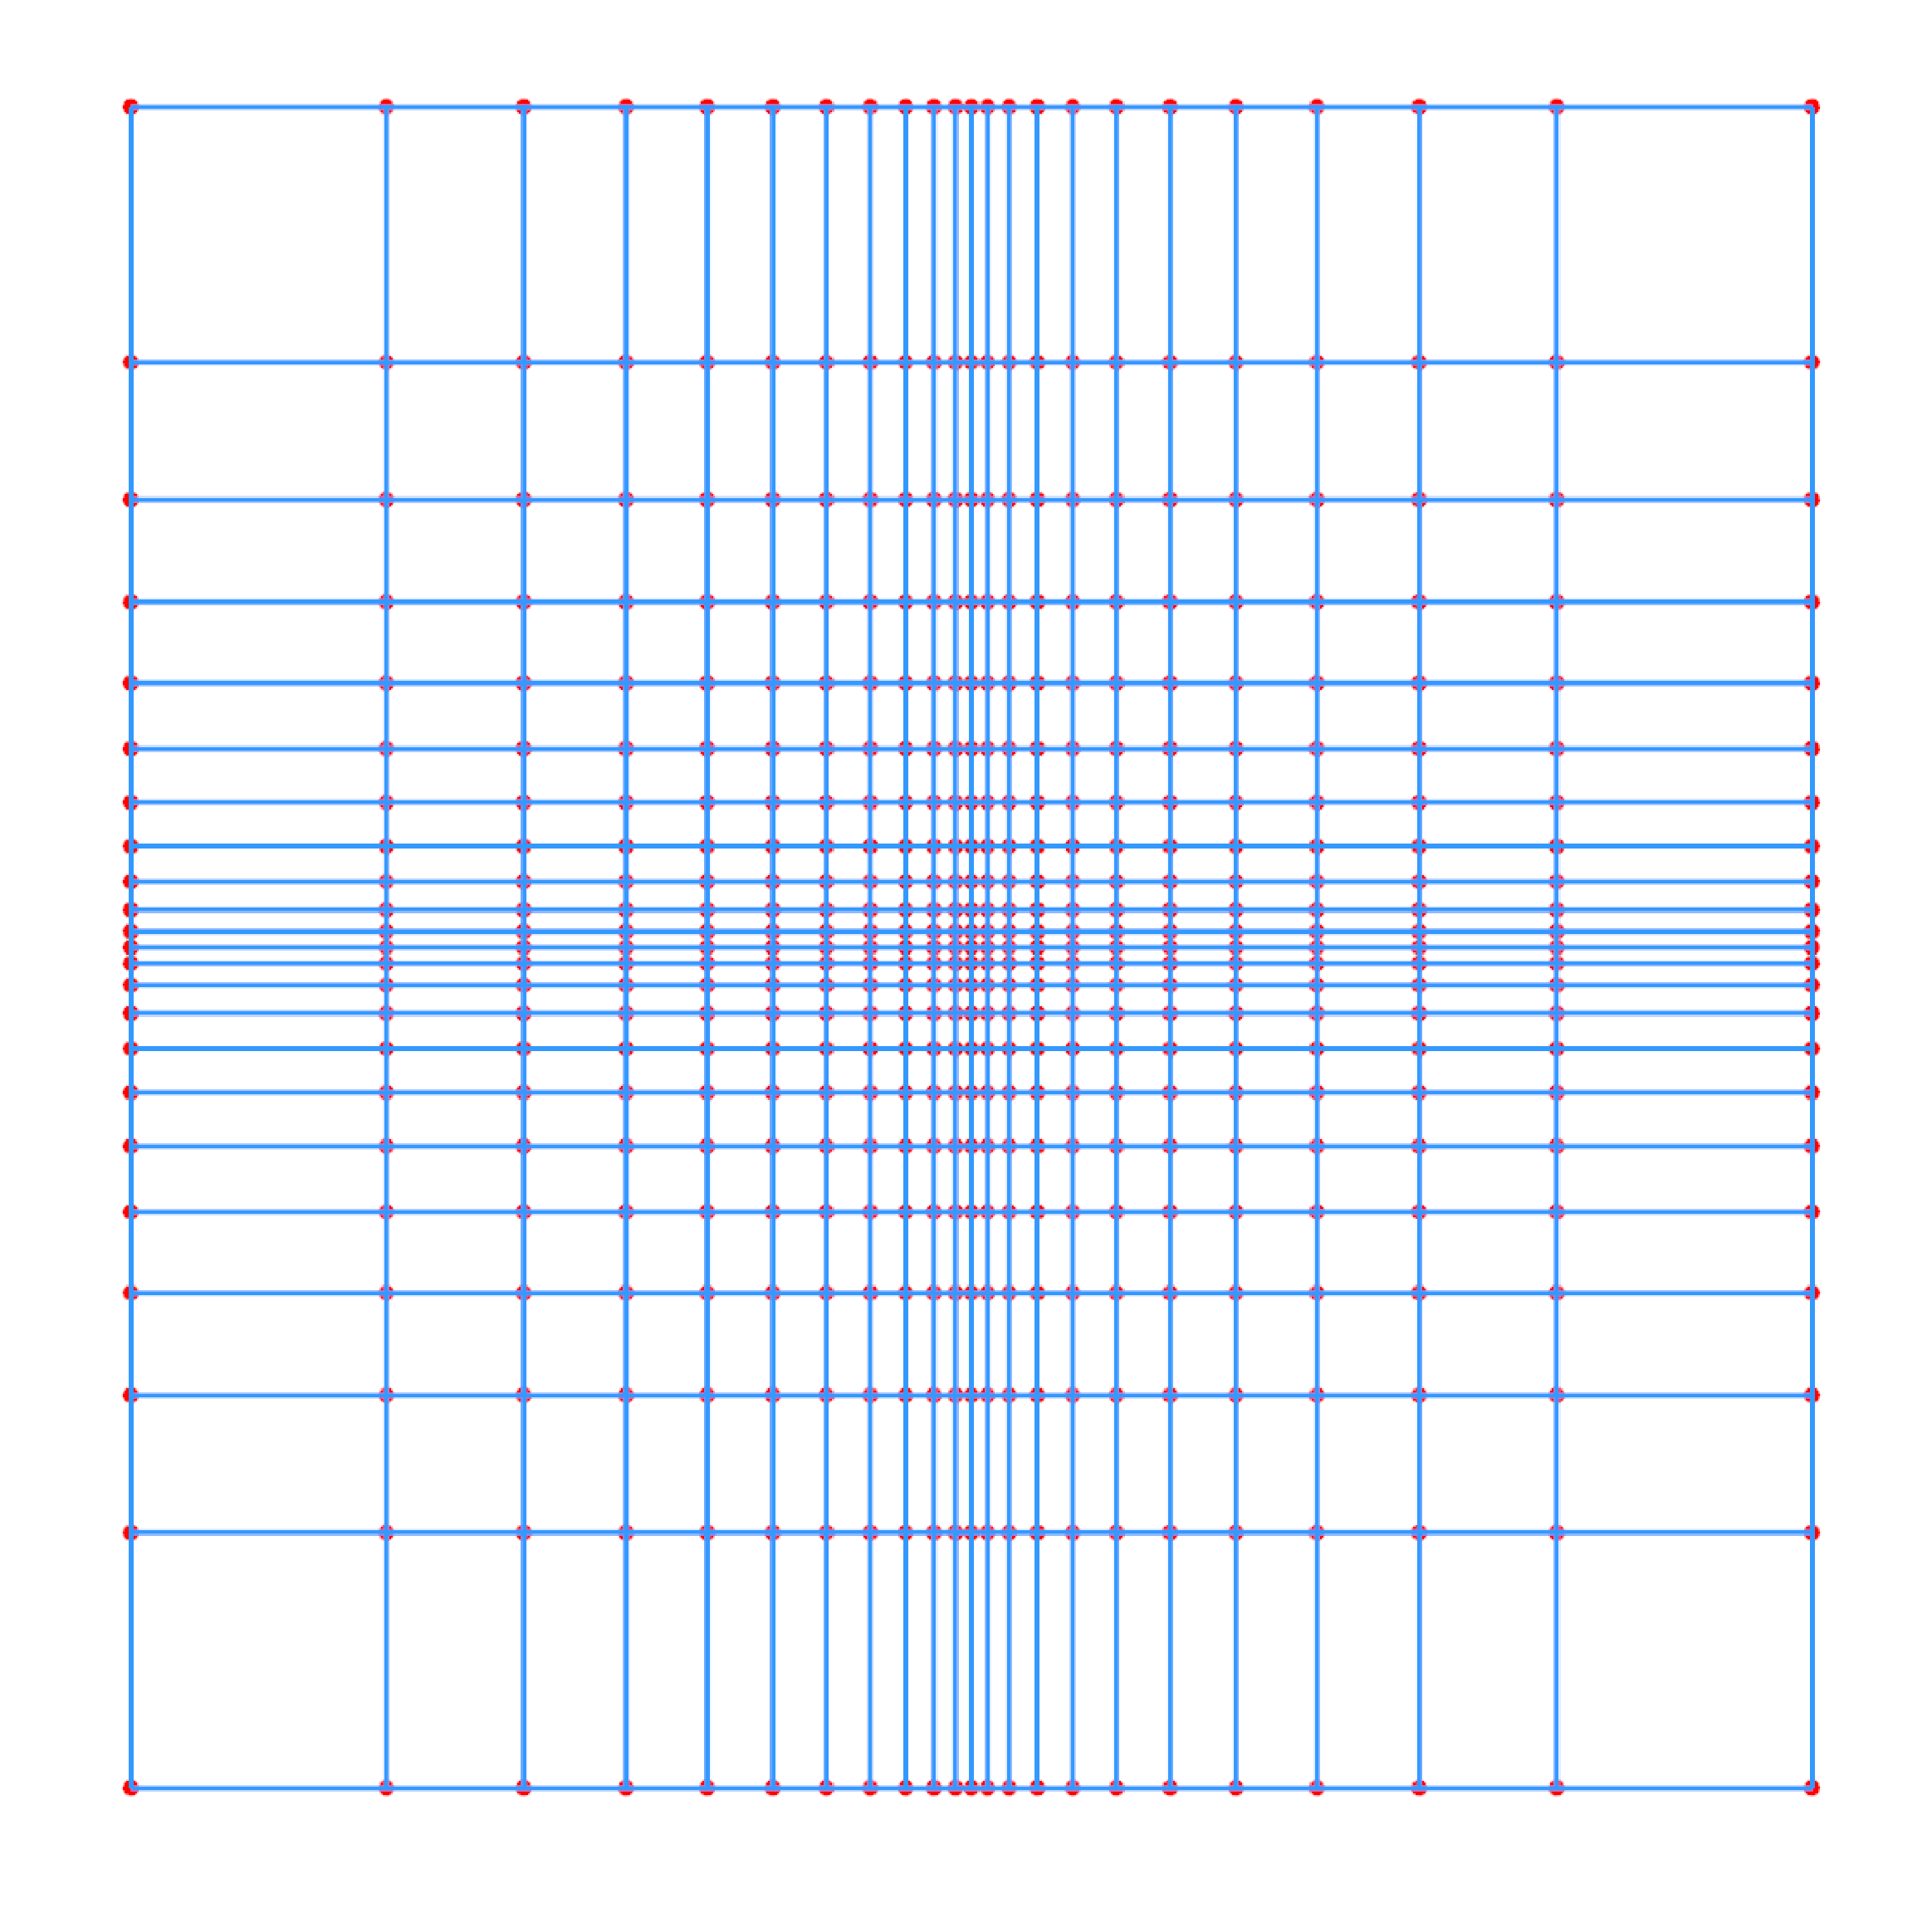
\epsfig{file = square_s-rep.eps, width = 3cm}}
% \subfigure[Circular log grid]{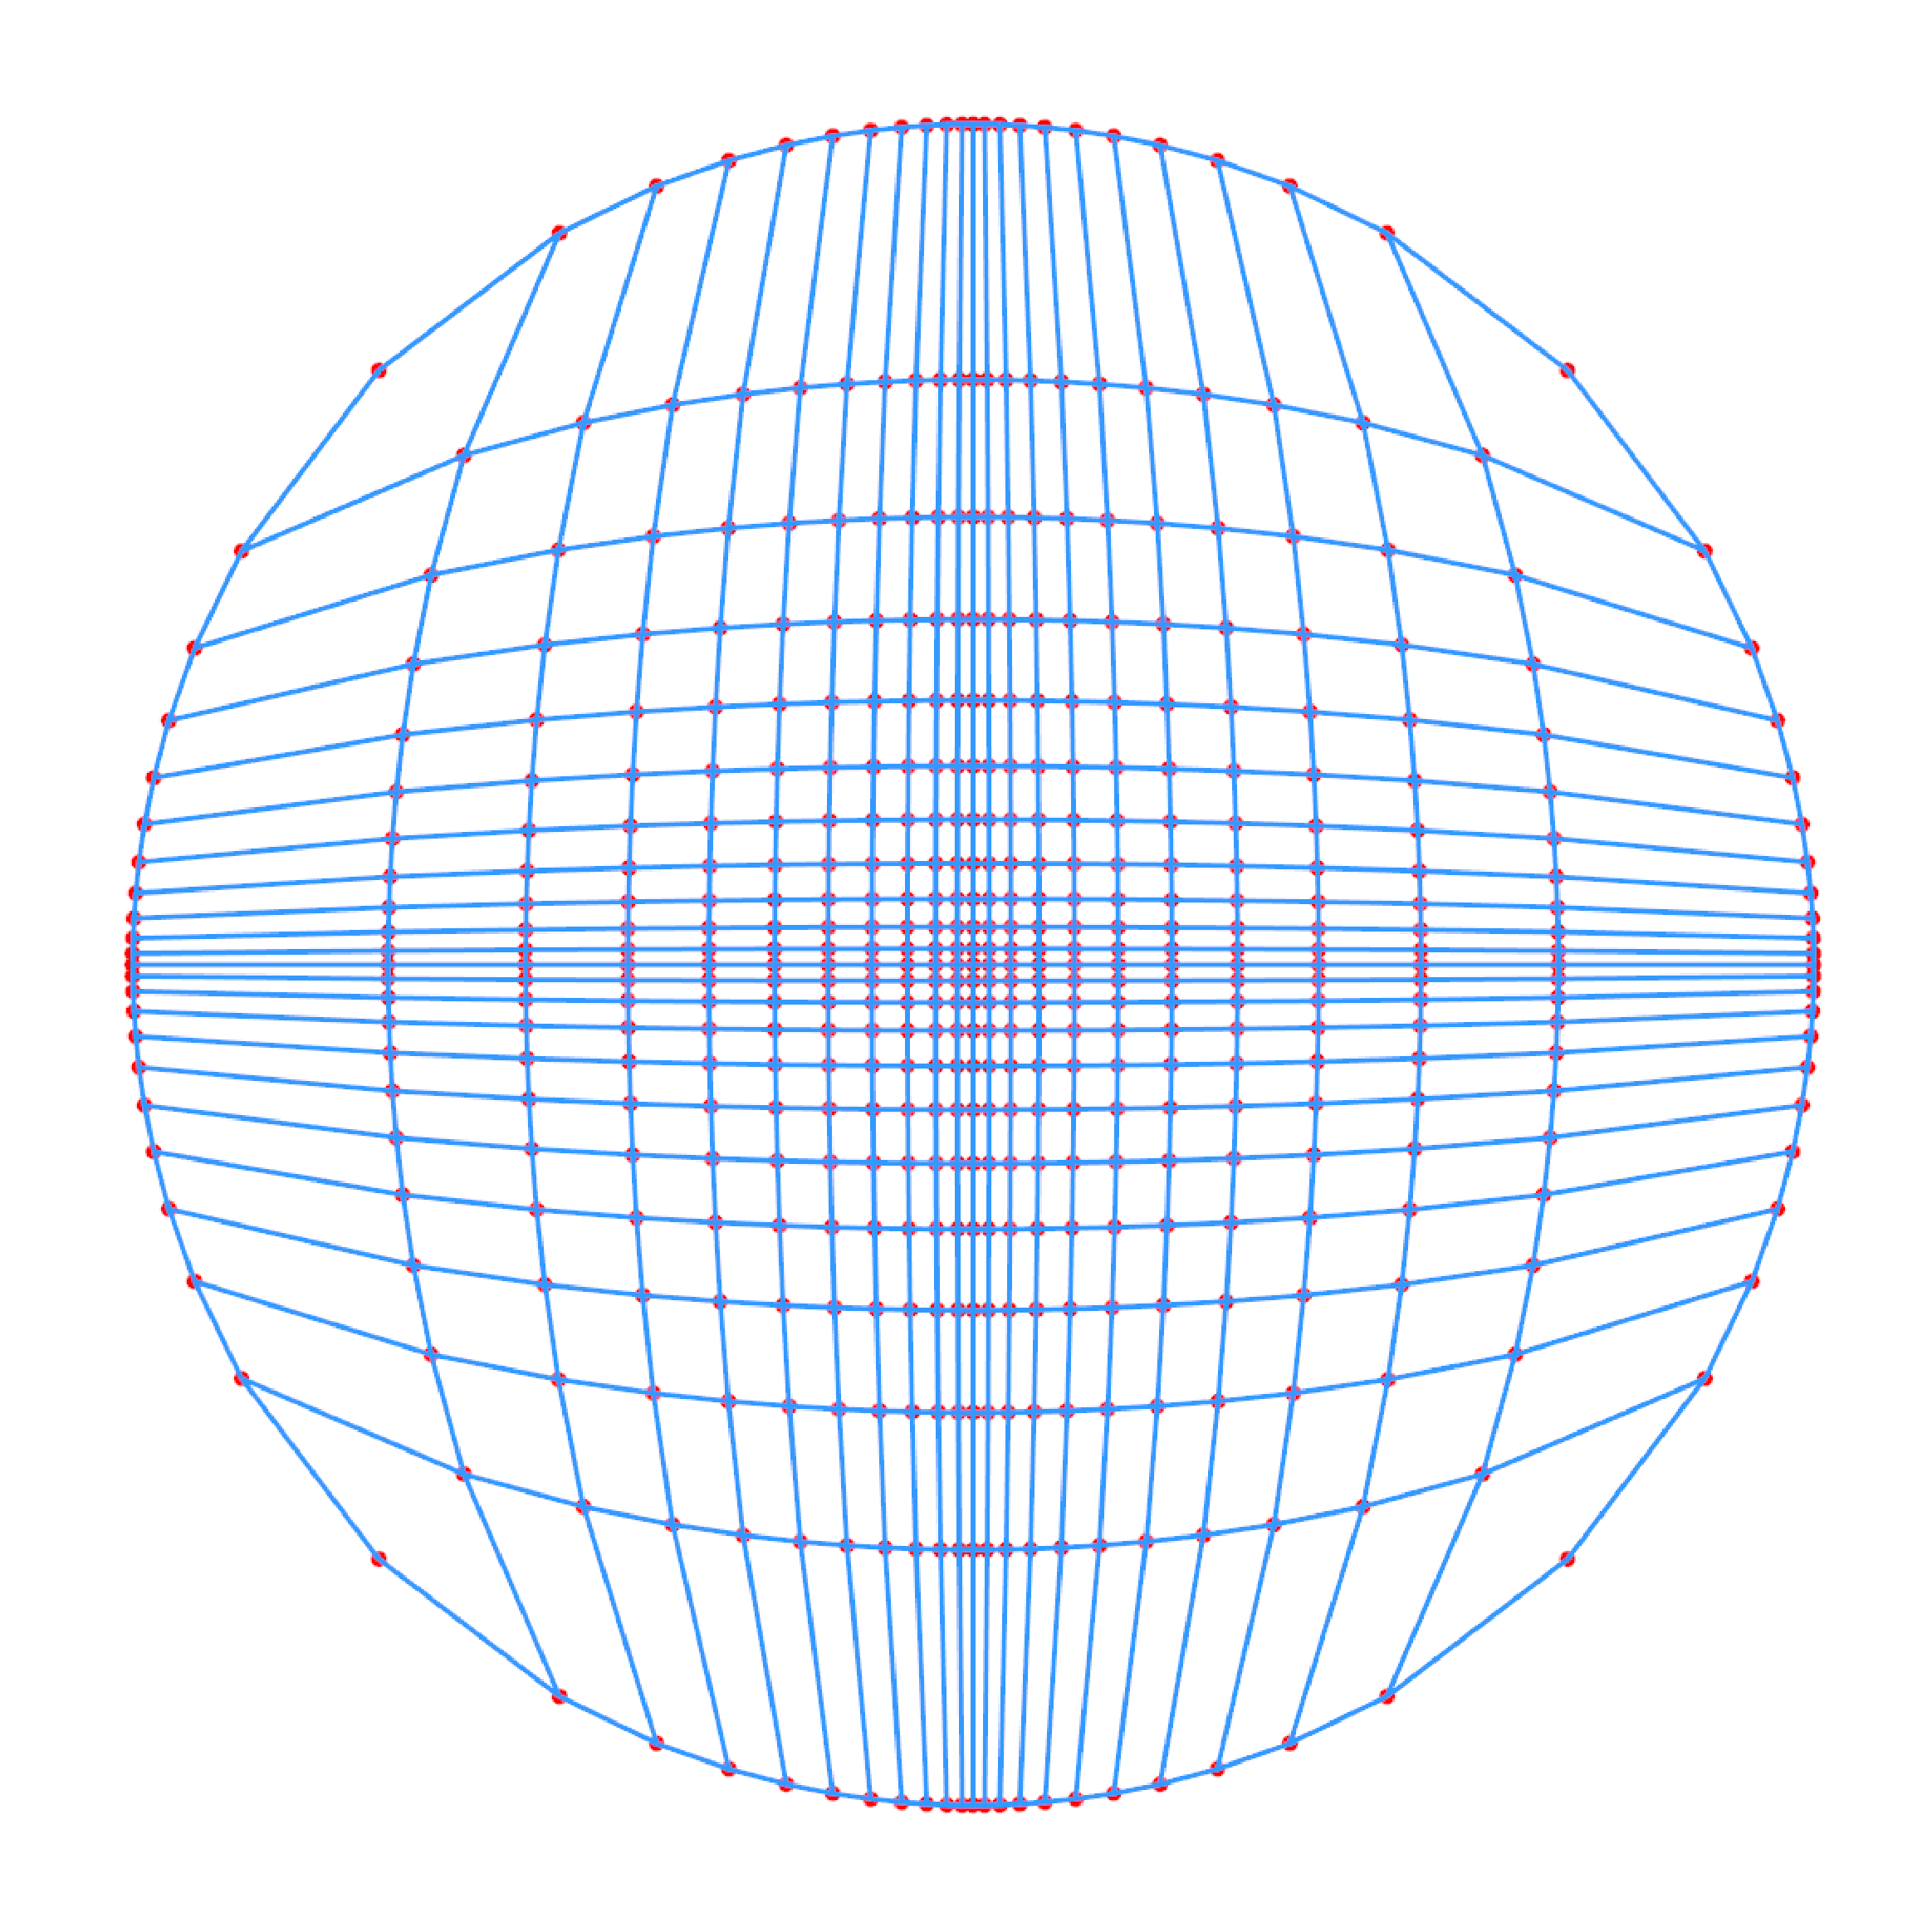
\epsfig{file = circle_s-rep.eps, width = 3cm}}
% \caption{A square grid transformed into a circle on the plane.}
% \label{fig:GridTypes} 
% \vspace{-0.1cm}
%\end{figure}

The following section explains how to project the transformed grid to the sphere.
Figure \ref{fig:SphereSamplingSphere} shows the results of mapping a regular-grid and log-grid on the sphere. 

\subsection{S-rep projection from the plane to the sphere}
\label{sec:StereographicProjection}

Once the ``circular log grid'' is created, the projection 
finds the corresponding positions on the sphere. 
Equation \ref{equ:stereoprojection} shows how the projection is done where $X = L(S(x'))$ and $Y = L(S(y'))$.

\begin{equation}  
	\begin{array}{lcc}
	    xs & = & 2X/(1 + X^2 + Y^2) \\
	    ys & = & 2Y/(1 + X^2 + Y^2) \\
	    zs & = & (-1 + X^2 + Y^2)/(1 + X^2 + Y^2)
	\end{array}
  \label{equ:stereoprojection}
\end{equation}

\begin{figure}[h!]
 \centering 
 \subfigure[Regular grid]{\epsfig{file = regularGridNorthPole.eps, width = 3.5cm}
			   \epsfig{file = regularGridSouthPole.eps, width = 3.5cm}}
 \subfigure[Log grid]{\epsfig{file = logGridNorthPole.eps, width = 3.5cm} 
		       \epsfig{file = logGridSouthPole.eps, width = 3.5cm}}
 \subfigure[Circular log grid]{\epsfig{file = circularLogGridNorthPole.eps, width = 3.5cm} 
		       \epsfig{file = circularLogGridSouthPole.eps, width = 3.5cm}}
		      
 \caption[Sphere's north and south pole sampling.]{The north (left) and south (right) poles are sampled using a regular,  a log grid and a circular log grid. 
						     The log grid sampling maps more points towards the south pole, and the circular grid 
						     produces the spherical cap opening in the representation.}
 \label{fig:SphereSamplingSphere}  
\end{figure}

Figure \ref{fig:SphereSamplingSphere} shows how the points from the regular grid and the log grid map 
on a sphere. The latter has better hub distribution on the sphere and produces a better s-rep of the cortex. 

Once the hub positions are sampled on the sphere, a fitting procedure to the spherical data provided by \textit{Freesurfer} is done.

\subsection{Fitting the s-rep to \textit{Freesurfer's} data}

At this point there are two spherical representations. 
The first one corresponds to a cortex;
the second one corresponds to the s-rep's SS.

To fit the s-rep to the spherical representation of the cortex,
each hub position is used as input to search for a set of closest points on 
the spherical representation of the cortex.
The searching procedure uses as standard closest neighborhood search algorithm 
with kd-trees. The kd-tree quickly locates the closest points on the sphere from \textit{Freesurfer}.

The folding procedure in the following section uses the points found
and their relationship to the GM and WM surfaces in order to fold the s-rep into the cortex.

\subsection{Folding the s-rep: from the sphere to the cortex}

%\begin{figure} 
% \centering 
% \subfigure[Circular grid]{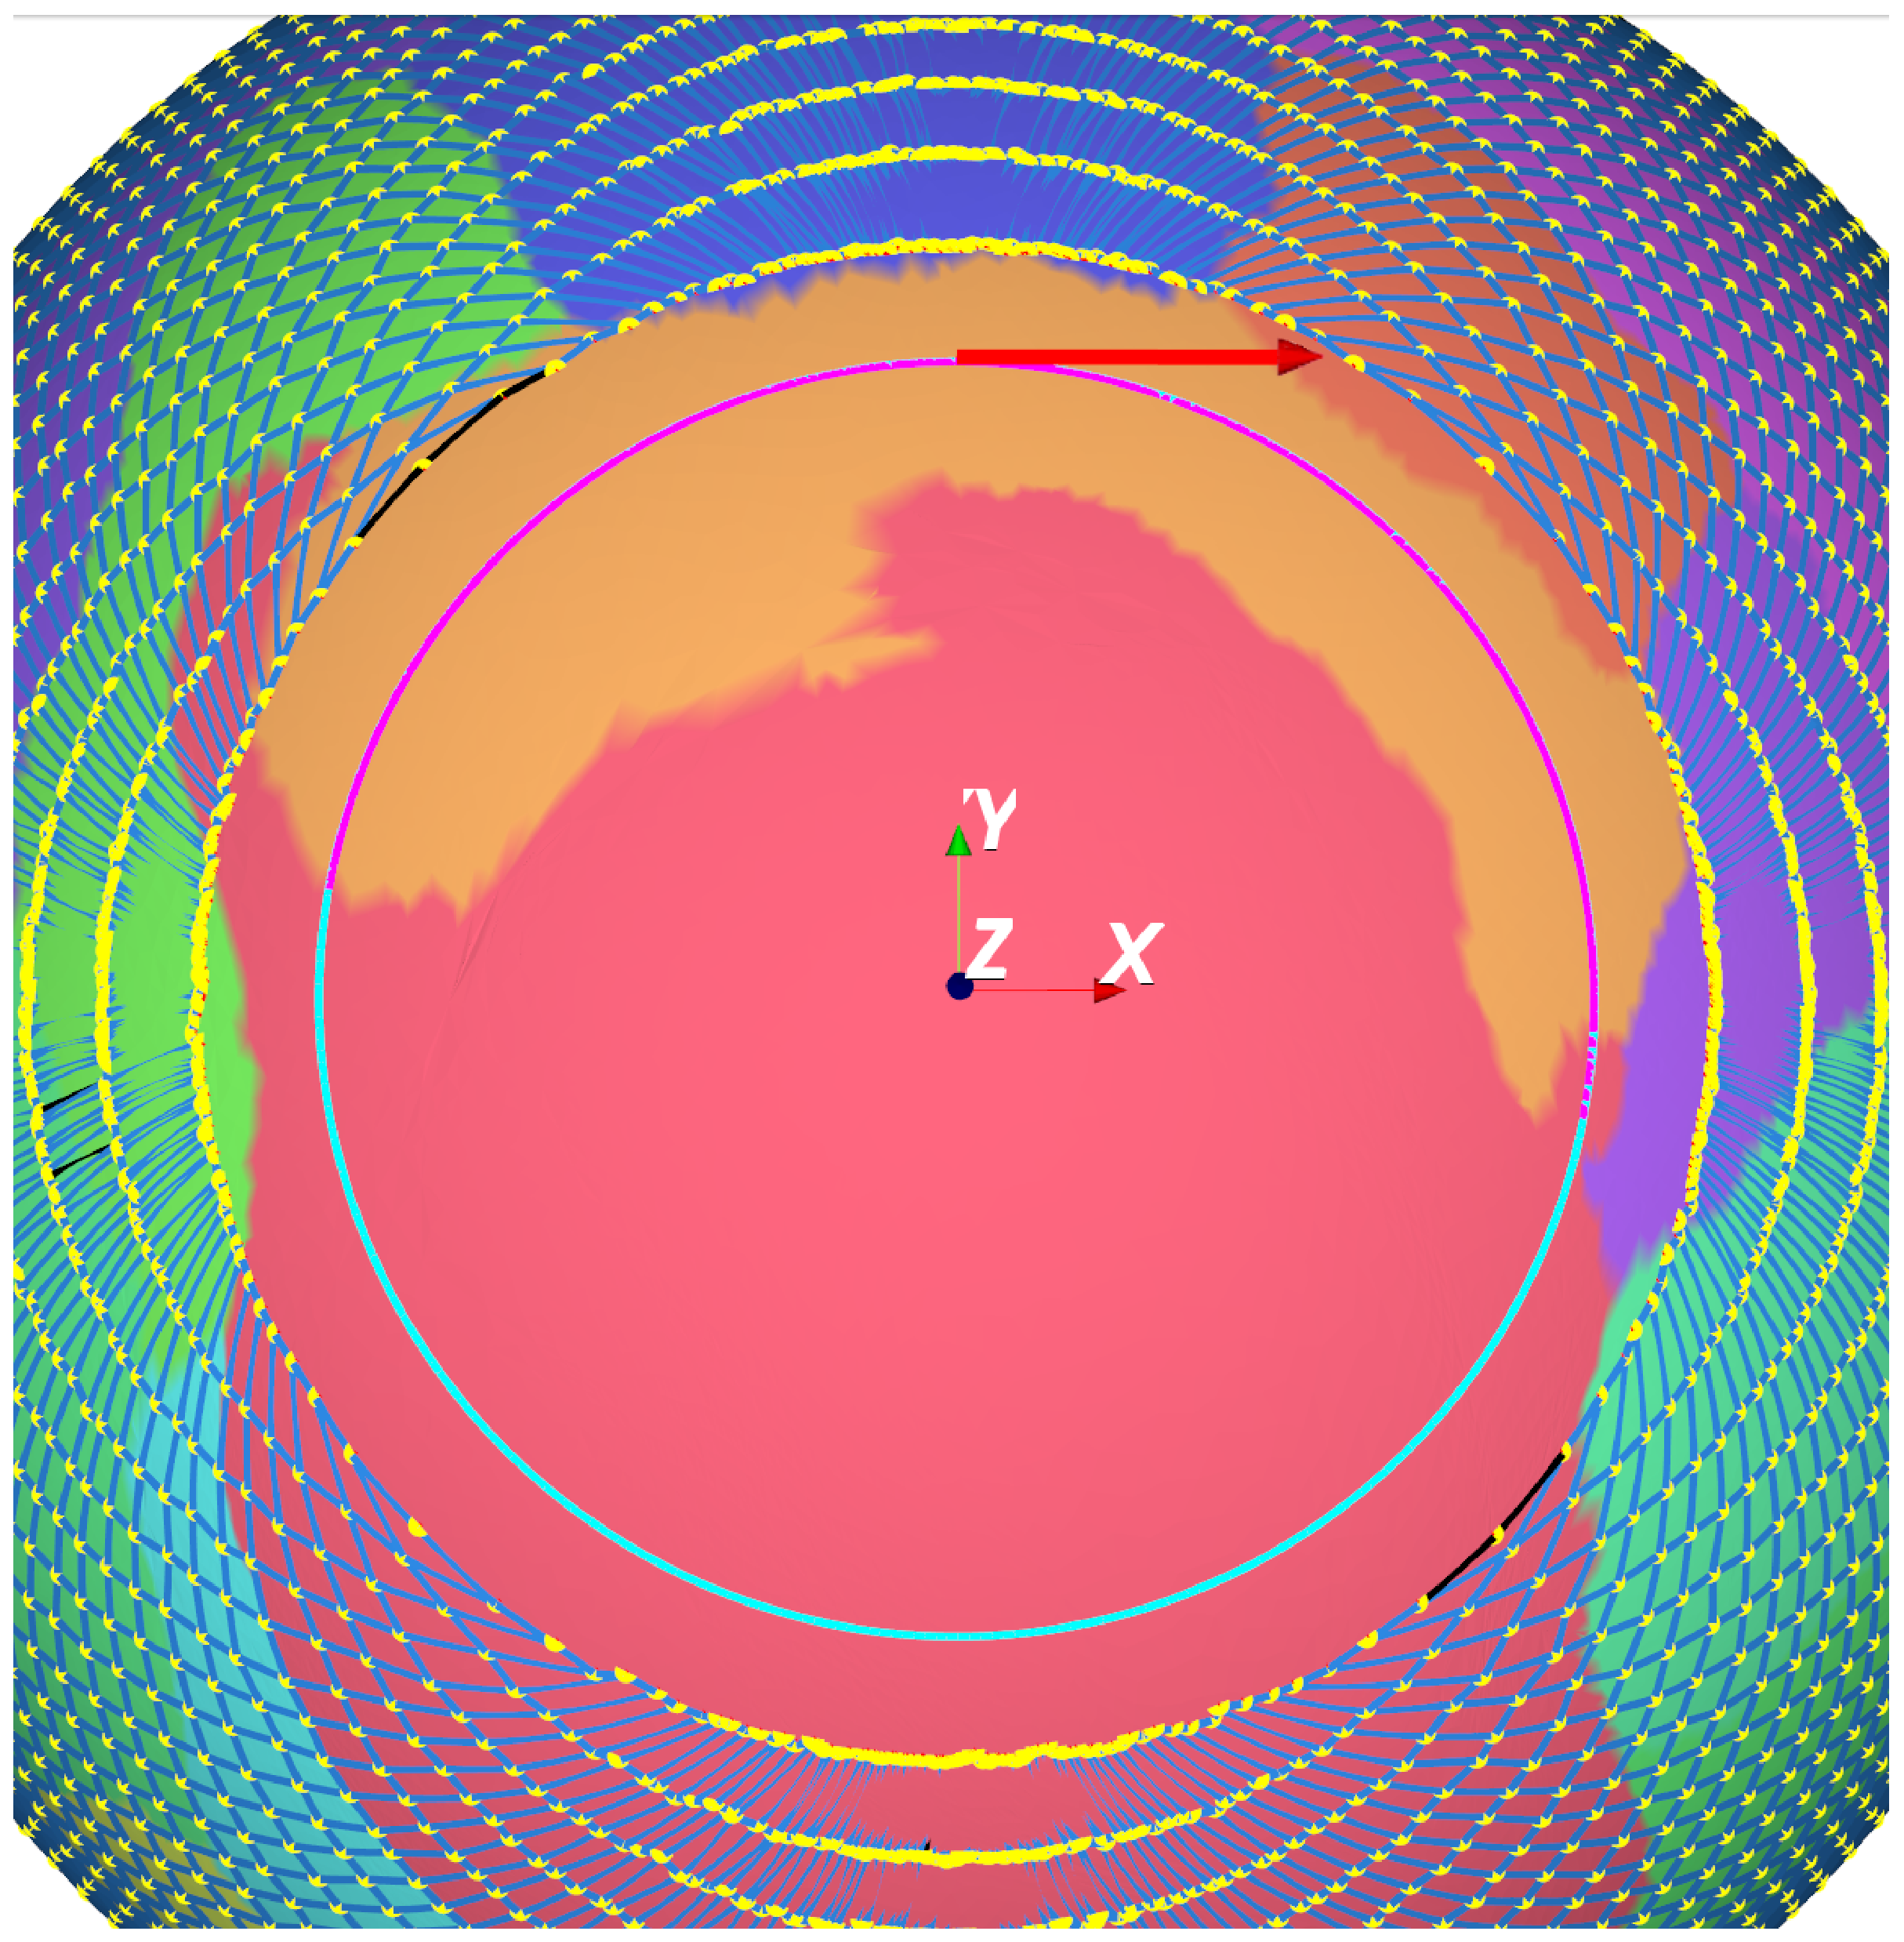
\epsfig{file = fittedSrepSphereCircularGrid.eps, width = 2.75cm}
%			   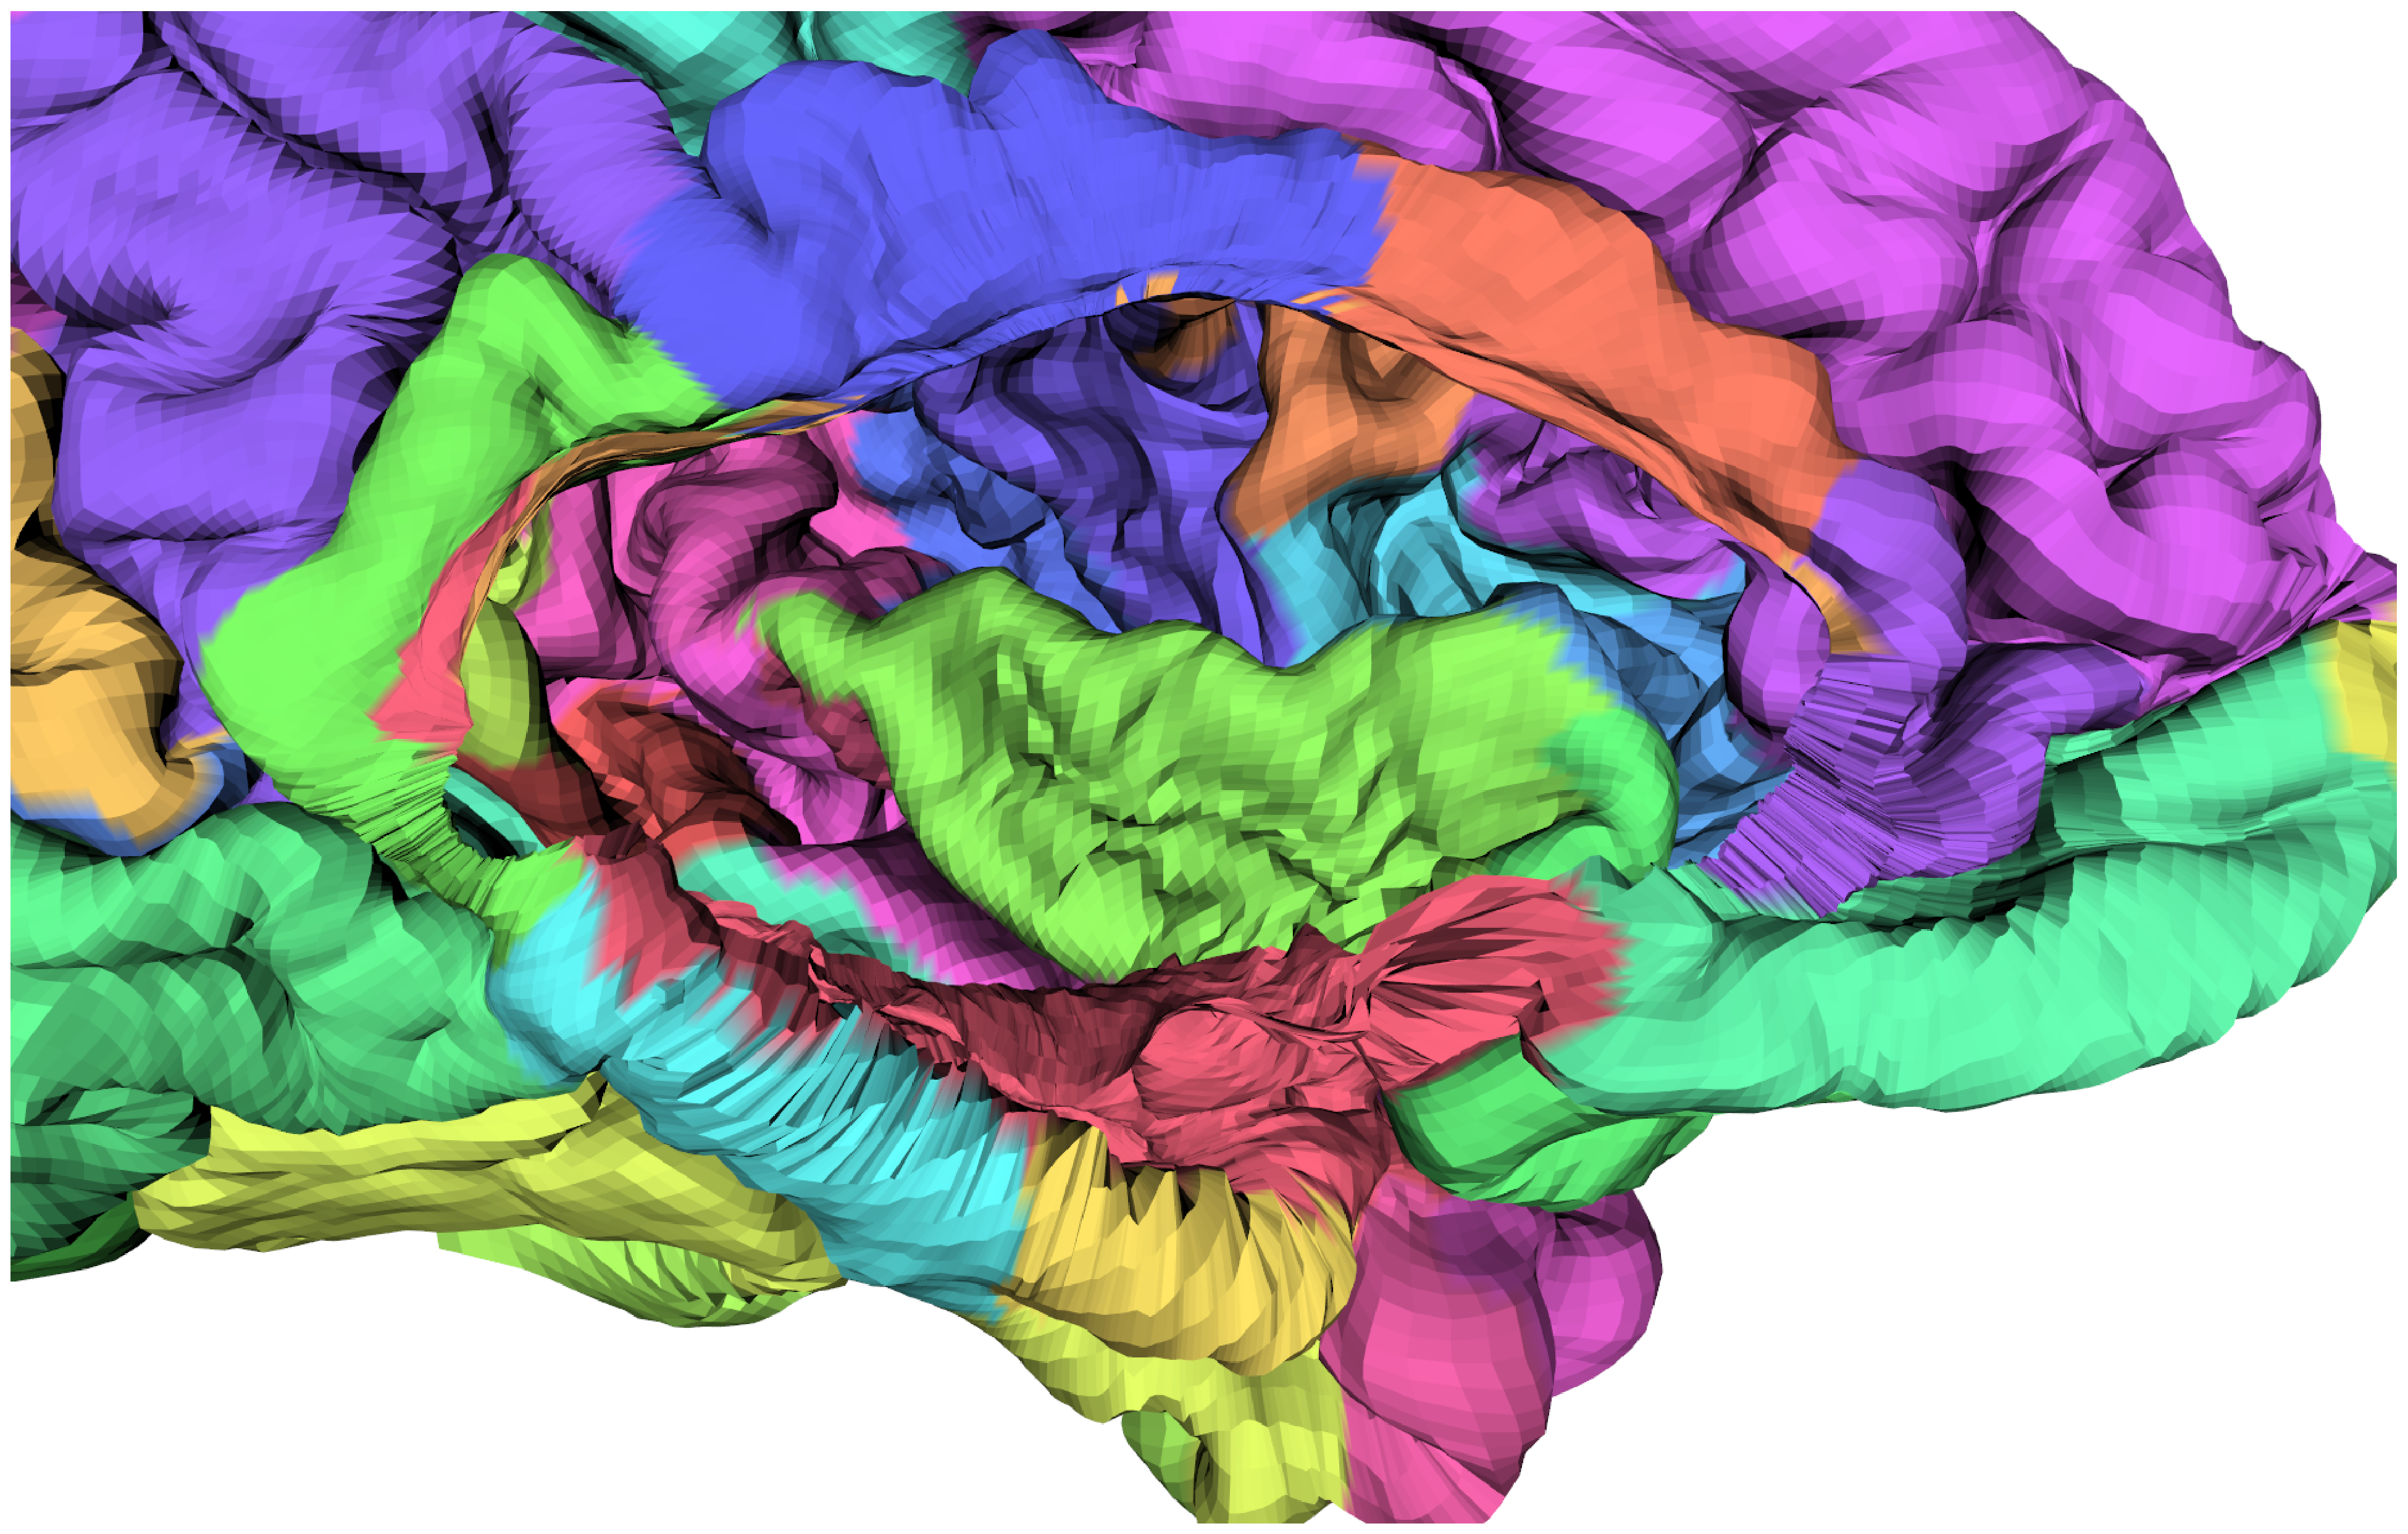
\epsfig{file = fittedSrepCircularGrid.eps, width = 3cm}}
% \subfigure[Square grid]{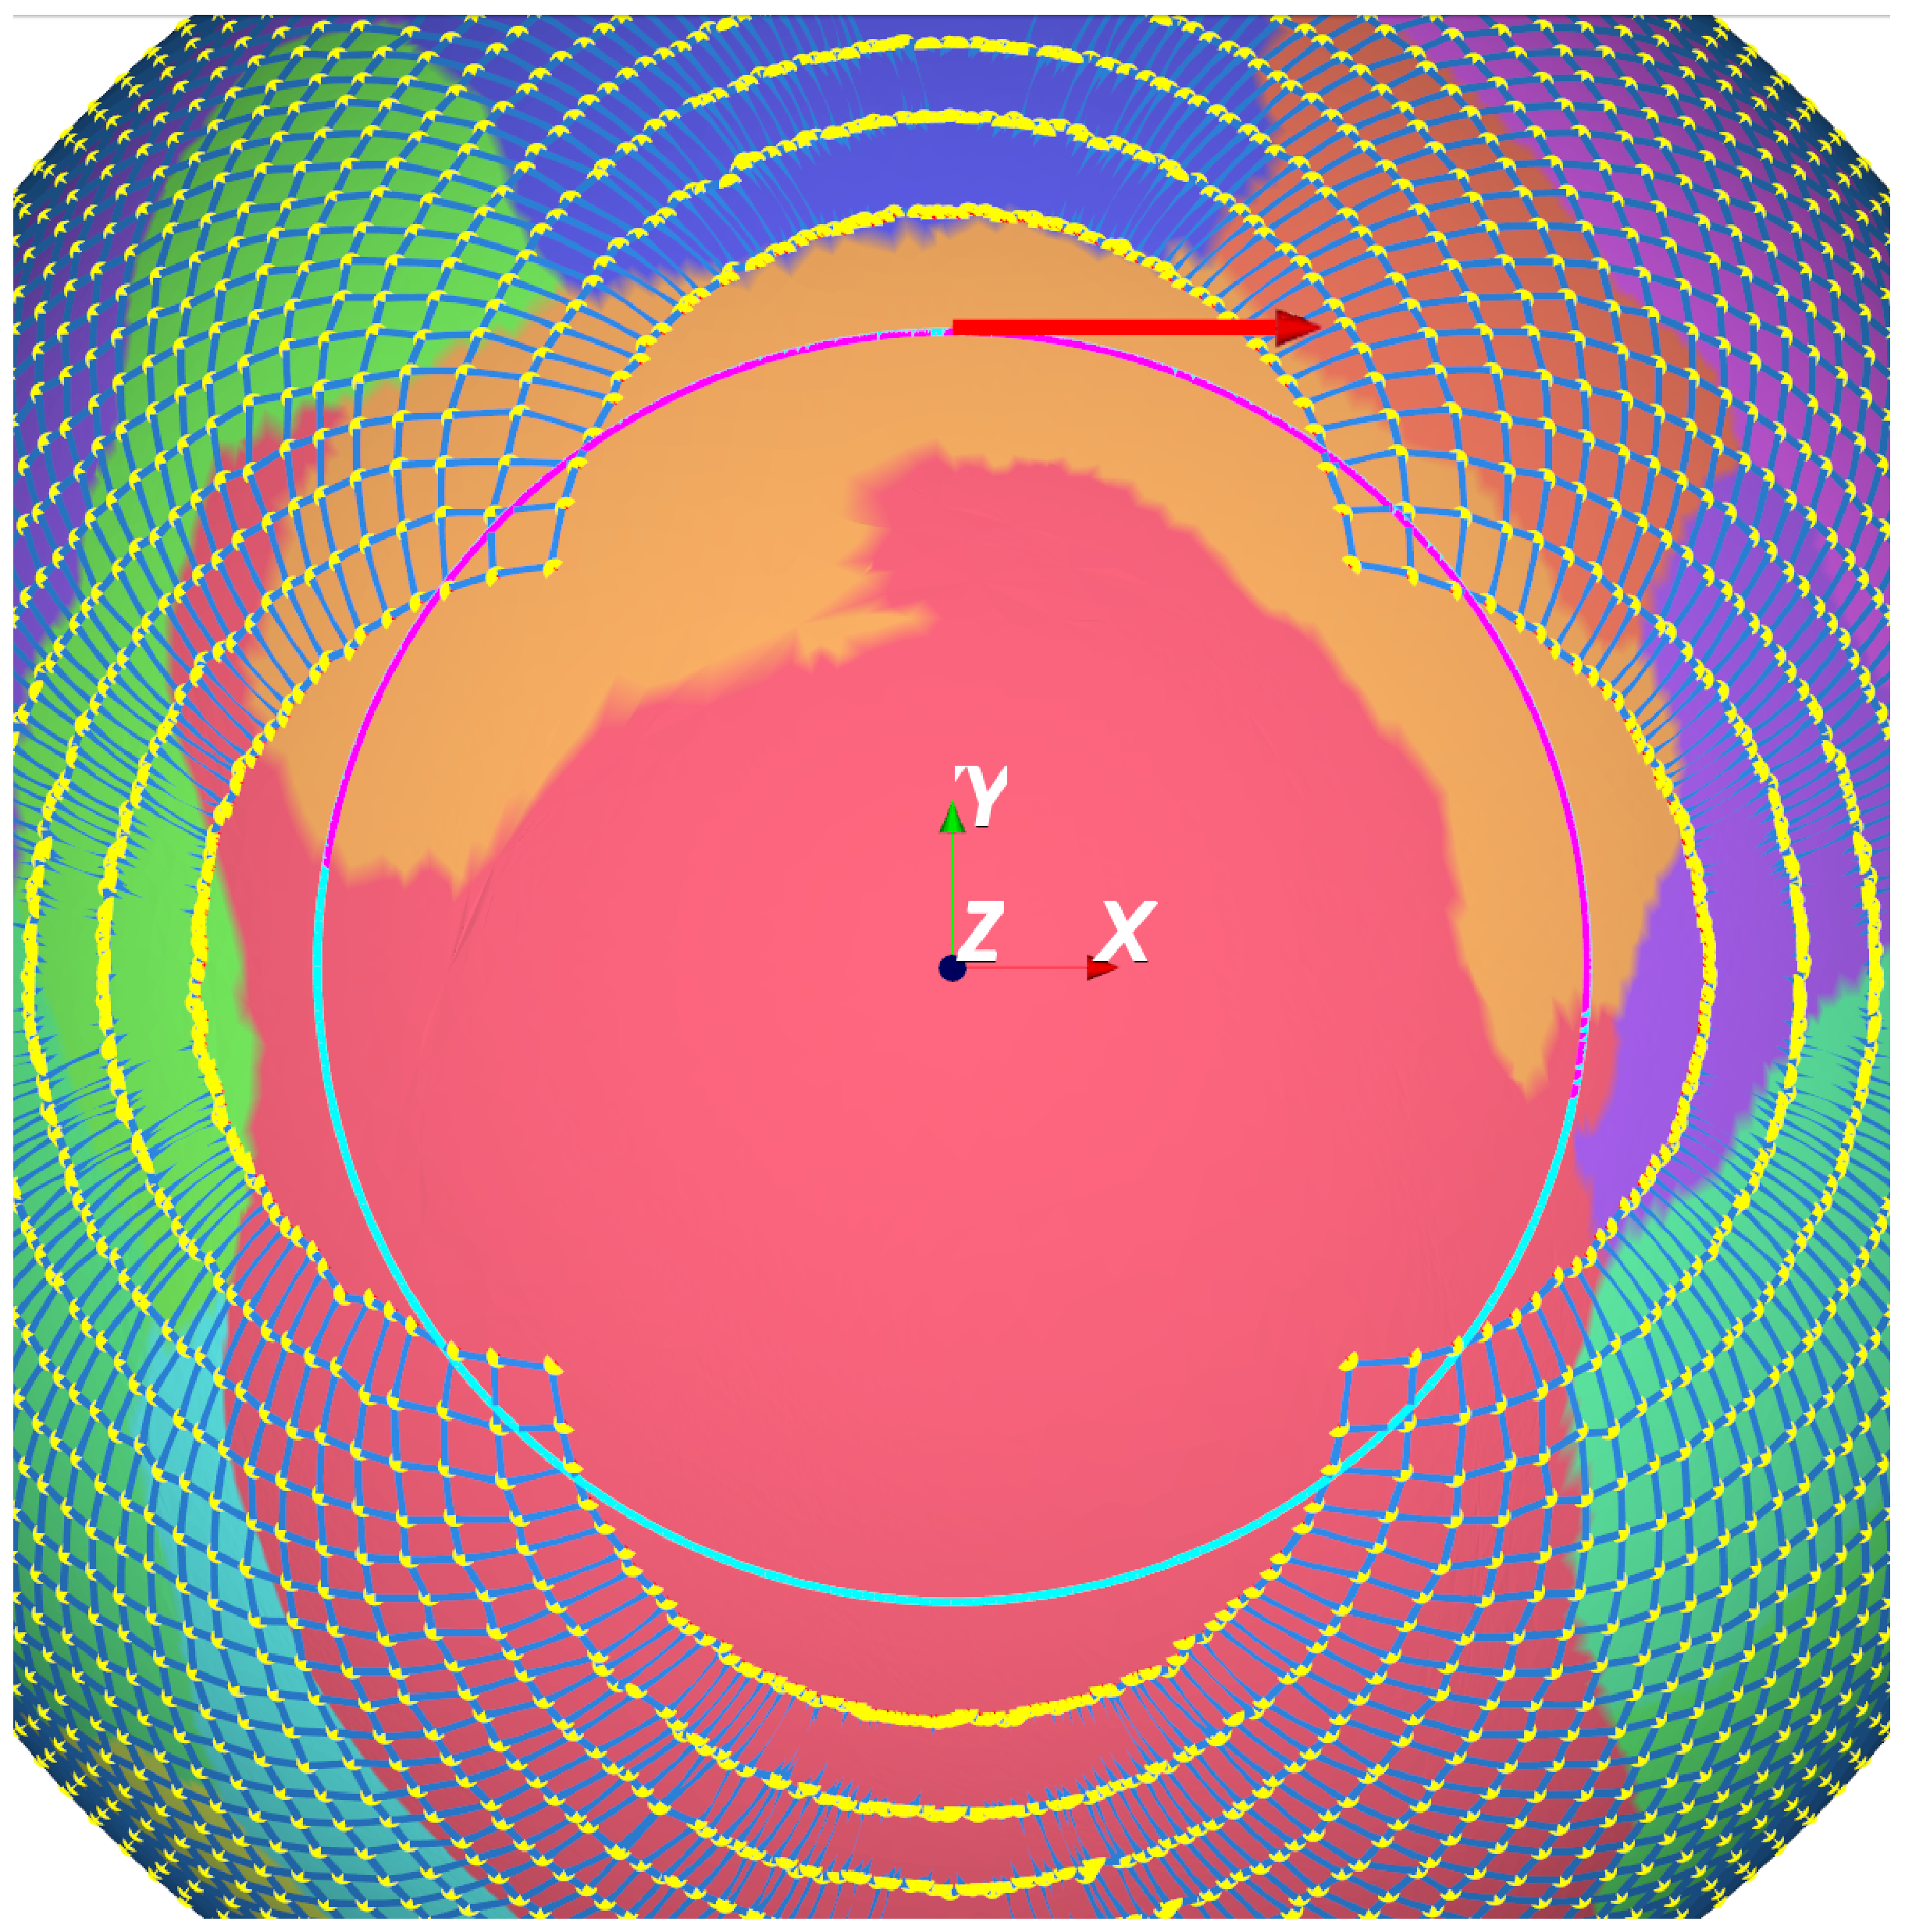
\epsfig{file = fittedSrepSphereSquareGrid.eps, width = 2.75cm} 
%		       \epsfig{file = fittedSrepSquareGrid.eps, width = 3cm}} 
% \caption{The best circle is shown in cyan, the projected points in magenta (on top of the best circle).
%	  The north pole is the center point of the best fitting circle, it is used to rotate the sphere to the north pole. 
%	  The mean of the projected points is found on the circle and is used to calculated a tangent, which is later used to 
%	  calculate a second rotation to align the data with the x axis. On figure (b), the regions highlighted in red correspond 
%	  to the corners of the grid.}
% \label{fig:BestCircle}  
%\end{figure}

The s-rep is folded into the cortex
using the points found on the sphere and
the cortical widths given by \textit{Freesurfer}. 

The following penalties minimize an objective function for each hub:

\begin{enumerate}
 \item The hub's distance to the GM and WM surfaces (~half the cortical width).
 \item The top spoke's tip distance to the GM surface.
 \item The bottom spoke's tip distance to WM surface.
 \item The normal of the SS (see Equation \ref{equ:sheetNormal}) to the normal of the WM surface.
 \item The normal of the SS to the normal of the GM surface.
\end{enumerate}


%\begin{equation}
% \hat{s_{rep}(i)} = \operatorname*{Arg\,min}_{p_i, s^{-1}_i, s^1_i} \sum_{j=1}^{k} || Cp(j) - p_i || + \left \{ \begin{array}{ll}
%                                                                                                                 ||Cp(j) - (p_i +  s^{-1}_i)||, & Cp(j) \in WM \\
%                                                                                                                 ||Cp(j) - (p_i +  s^{1}_i)||, & Cp(j) \in GM
%                                                                                                                \end{array} \right .
%                                                                                                     + || (s^{1}_i - s^{-1}_i) - NCp(i) ||
%\end{equation}

The procedure folds back the s-rep that was sampled on the spherical space to the original shape of the cortex. 
After the folding, the topology of the s-rep is preserved. 
In other words, each of the quads that build the skeletal structure 
are correctly oriented on the folded form of the cortex. 
Moreover, both top and bottom spokes point towards the GM and WM surfaces respectively. The width of the
spokes is also determined.

The interpolation mechanisms described in Section \ref{sec:s-repImplementation} can 
be used to produce the WM and GM surfaces. 
Since the implied surfaces are not equivalent to the original ones, the following section evaluates 
their quality. 

\section{Evaluation of the implied GM and WM surfaces}
\label{sec:Evaluation}

To evaluate if the surfaces are close enough to the original ones, 
a tool known as \textit{Meshvalmet} is used.
The tool uses the Hausdorff distance to estimate the difference between discrete 3D surfaces. 
The approach is based on \cite{aspert_mesh:_2002}. It
calculates the mean distance error from each vertex of the reference surface to 
a target one, in this case, the interpolated surface against the original surface. 
The comparison is done separately on the GM and WM surfaces.
The sampling step is set to $0.1$ and an absolute distance measure is used.
By lowering the sampling step and using the 
absolute distance, the accuracy of \textit{Meshvalmet} is increased.

Analyzing the results of \textit{Meshvalmet} 
yields a set of parameters to generate the best possible representation 
for all subjects. 
The parameters to set for the s-rep are size and sampling step on the sphere.
The following section analyzes the size of the s-rep.

\subsection{Best s-rep size}
\label{sec:s-repsize}

\begin{figure}[!h]
 \centering 
 \subfigure[GM surface]{\epsfig{file = lh_greyMatterGridSize.eps, width = 7.25cm}}
 \subfigure[WM surface]{\epsfig{file = lh_whiteMatterGridSize.eps, width = 7.25cm}}
 \caption[GM and WM surface mean error: grid size.]{Mean error using different grid size of the s-rep.}
 \label{fig:GridSize} 
\end{figure}

The first parameter to set is the size of the s-rep. This is based on different criteria
such as reducing the number of points in the original data. A typical cortical surface contains $130,000+$ vertex.
By using an s-rep of $160^2$ atoms, the information is reduced by $~40\%$, \textit{i.e}, 
$76.800$ tuples including the hub positions plus both spoke directions.
%Reducing the information not only allows to produce compact representation of the data but it also allows the use of new statistical tools.

Figure \ref{fig:GridSize} shows the mean error using s-reps of different sizes, tested on 8 different subjects. 
The following analysis uses a grid of $160^2$ atoms for all cases.

\subsection{Best s-rep sampling}
\label{sec:minvalue}

The second parameter to set is the initial value for the log scale sampling on the grid.
This parameter controls how the hubs will distribute on the sphere. A value close to $0$ will 
map a larger number of points towards the south pole. 
Figure \ref{fig:AverageCell} shows the average area of the quads that compose the skeletal locus of the s-rep and their SD (standard deviation).
Notice that for values greater that $0.04$, the SD increases rapidly.
Figure \ref{fig:InitialLogValue} shows the mean error of the interpolated surfaces for different $Min$ values.
According to the analysis, values between $0.01$ and $0.4$ seem reasonable as 
the minimum error overall cases for the surfaces is found inside this range.
The $Min$ value is set to $0.02$
in order to increase the regularity of the quads and 
lower the mean error of the surface.
This value produces the best results over all subjects used in the analysis. 

\begin{figure} 
 \centering  
 \epsfig{file = lh_averageCellArea.eps, width = 9cm}
 \caption[Average area of an srep's quad.]{Average quad area of the s-rep with standard deviation for different $MIN$ values of the log scale.}
 \label{fig:AverageCell}  
\end{figure}

\begin{figure} 
 \centering 
 \subfigure[GM surface]{\epsfig{file = lh_greyMatterLogScale.eps, width = 7.25cm}}
 \subfigure[WM surface]{\epsfig{file = lh_whiteMatterLogScale.eps, width = 7.25cm}}
 \caption[GM and WM surface mean error: log scale.]{Mean error of the GM and WM surfaces for different $MIN$ values of the log scale.}
 \label{fig:InitialLogValue} 
\end{figure}


Figure \ref{fig:InterpolatedCortex} shows the interpolated cortex for both hemispheres. 
The coloring on the surfaces are set according to the cortical
parcellation of the neuroanatomical structures at each location in the cortex. 
%Each atom has the corresponding label found on the spherical surface.
%During the interpolation, each new point is labeled according to a voting scheme using the labels of the closest neighboring atoms.

\begin{figure}
 \subfigure[Original surfaces.]{\epsfig{file = lh_whiteMatterOriginal.eps, width = 8cm}
			   \epsfig{file = rh_whiteMatterOriginal.eps, width = 8cm}}
 \subfigure[Interpolated surfaces.]{\epsfig{file = lh_whiteMatterInterpolated.eps, width = 8cm}
			   \epsfig{file = rh_whiteMatterInterpolated.eps, width = 8cm}}
 \caption[Comparison of the interpolated and original WM surfaces.]{Comparison of the original and interpolated WM surfaces for the left and right hemispheres.
	  The s-rep has $160^2$ atoms. The interpolated surfaces seem to have wrinkles at some places 
				      but according to the error measurement, they are close to the original ones. 
	                             Moreover, modeling the cortex via s-reps offers new capabilities such as the local coordinate system inside the structure.
	                             This new set of capabilities are not available in the regular representation.}
 \label{fig:OriginalCortex}
\end{figure}
\begin{figure} 
 \subfigure[Original surfaces.]{\epsfig{file = lh_greyMatterOriginal.eps, width = 8cm}
				  \epsfig{file = rh_greyMatterOriginal.eps, width = 8cm}}
 \subfigure[Interpolated surfaces.]{\epsfig{file = lh_greyMatterInterpolated.eps, width = 8cm}
				  \epsfig{file = rh_greyMatterInterpolated.eps, width = 8cm}}
 \caption[Comparison of the interpolated and original GM surfaces.]{Comparison of the original and interpolated GM surfaces for the left and right hemispheres.			
	The s-rep has $160^2$ atoms. The interpolated surfaces seem to have wrinkles at some places 
				      but according to the error measurement, they are close to the original ones. 
	                             Moreover, modeling the cortex via s-reps offers new capabilities such as the local coordinate system inside the structure.
	                             This new set of capabilities are not available in the regular representation.}
 \label{fig:InterpolatedCortex}  
\end{figure}

In the following section, the s-rep of the cortex is used to evaluate
the changes of cortical width using synthesized data from a base model. 

%\begin{figure}
% \vspace{-0.2cm}
% \centering 
% \subfigure[Gray matter surface]{\epsfig{file = lh_greyMatterInterpolationLevel.eps, width = 6cm}}\\
% \subfigure[White matter surface]{\epsfig{file = lh_whiteMatterInterpolationLevel.eps, width = 6cm}}
% \caption{Mean error for different start points of the log scale.}
% \label{fig:InterpolationLevel}
% \vspace{-0.1cm}
%\end{figure}

\section{Shape statistics of the cortex using CPNS}
\label{sec:Statistics}

%Statistics on objects has been applied to quite a variety of types of geometric model derived from the boundary
%cases:
%1. PCA has been applied to boundary point distribution models (\cite{cootes_training_1992}, \cite{kurtek_parameterization-invariant_2011}). 
%Kendall \cite{kendall_shape_2009} showed this is not correct as this type of models live in a space
%formed by a Cartesian product of a Euclidean space and high dimensional spheres. 
%Further developments yield a technique called PGA (principal geodesic analysis) \cite{angeles_generalized_2010} 
%which produced better statistics than PCA but still not satisfactory. 
%2.
%Deformation-of-atlas models, where the displacement of each voxel in the atlas
%is provided \cite{pennec_statistical_2009}, \cite{arsigny_log-euclidean_2006}). These models have enormous dimension, 
%and the statistical analysis is expensive and unstable with respect to the sampling
%into training cases and to noise in those training cases.
%3.
%Implicit models, such as level surfaces of pseudo-signed-distance functions \cite{clark_automatic_1998},
%that do not live in Euclidean feature spaces but are often analyzed (by PCA) as if they did.
%4.
%Skeletal models such as s-reps, live in abstract manifolds that are curved, 
%composed by a Cartesian product of a Euclidean space and a collection of spherical spaces.
%This type of models have many advantages as they capture information of the surface
%and the interior of the object by providing a local frame and a coordinate system
%created from the atoms sampled on the medial sheet. 
S-reps live in abstract manifolds that are curved,
composed by a Cartesian product of a Euclidean space and a collection of spherical spaces.
Using s-reps to compute shape statistics should yield better shape descriptors as volumetric information
is included into the analysis. 
Previous studies on s-reps of hippocampi have shown 
CPNS to yield lower-dimensional shape space with an efficient collection of modes of variation better than 
PCA-based statistical analysis of other skeletal or non skeletal models \cite{pizer_nested_2012}, \cite{schulz_2012}.
The analysis on the cortex is challenging since its dimension is very high and shape variations could go undetected
by the approach.

\begin{figure}[tb]
  \centering
  \epsfig{file = lh_CPNS_Eigen30.eps, width = 8cm}    
  \caption[Mean modes of variation for the cortex.]{Mean modes of variation for the cortical representation.}
  \label{fig:Modes}   
\end{figure}


The objective of using CPNS on the cortex is to detect cortical thickness variations.
In order to do this a test case is made using a base s-rep and 60 models derived from the same one.
The cortical thickness is reduced in specific regions of the cortex.
The datasets are created by adding some Gaussian noise to the position of the model, and to every spoke direction and radii in the s-rep. 
Each sample is going to be further modified with a linear variation of the cortical thickness,
specifically on the superior frontal and superior temporal regions of the cortex.
Spoke lengths are reduced $30\%$ of their original length.
If CPNS produces modes of variation, then the first mode should be related to the cortical thickness reduction.

Figure \ref{fig:Modes} shows the plot of the eigenvalues describing the mean modes of variation computed with CPNS.
The first mode is responsible for the largest variation found in the dataset and should correspond to 
thickness reduction in the specific areas. 

Figure \ref{fig:EigenVariation} shows the evolution of the model by manipulating the first mode of
variation. In the figure, the regions of the superior frontal
and superior temporal of the cortex are thinner, and adjacent structures remain constant through the deformation.
This can also be verified by checking the average thickness as shown in figure \ref{fig:thickness}.
As expected the first mode corresponds to the cortical thickness variation.

\begin{figure*}  
  \centering
  \subfigure[$+1.5 \sqrt{\lambda_1}$]{\epsfig{file = lh_EigenVariation30+1.5.eps, width = 3.5cm}}
  \subfigure[$+1  \sqrt{\lambda_1}$]{\epsfig{file = lh_EigenVariation30+1.eps, width = 3.5cm}}
  \subfigure[$+0.5 \sqrt{\lambda_1}$]{\epsfig{file = lh_EigenVariation30+0.5.eps, width = 3.5cm}}
  \subfigure[Mean]{\epsfig{file = lh_EigenVariation30+0.eps, width = 3.5cm}}
  \subfigure[$-0.5 \sqrt{\lambda_1}$]{\epsfig{file = lh_EigenVariation30-0.5.eps, width = 3.5cm}}
  \subfigure[$-1 \sqrt{\lambda_1}$]{\epsfig{file = lh_EigenVariation30-1.eps, width = 3.5cm}}
  \subfigure[$+1.5 \sqrt{\lambda_1}$]{\epsfig{file = lh_EigenVariation30-1.5.eps, width = 3.5cm}}
  \epsfig{file = lh_EigenVariation30Bar.eps, width = 1.75cm}
  \caption[S-rep deformation using the first mode.]{Deforming the s-rep model using the first mode of variation and comparing it against the base s-rep.}
  \label{fig:EigenVariation}   
\end{figure*}

\begin{figure}[htb] 
  \centering
  \epsfig{file = lh_EigenVariation.eps, width = 9cm}    
  \caption[Average thickness of the cortex.]{Average thickness for some cortical regions in the cortex. The two regions changing through the deformation
           are the superiorfrontal and superiortemporal.}
  \label{fig:thickness}   
\end{figure}


\section{Conclusion}
\label{sec:Conclusion}

One of the major contributions of this work is to represent the cortex as a folded slab using s-reps. 
S-reps are able to model continuum space. This characteristic can be used 
for the following purposes:
to include information in the cortex at different scale levels; provide 
new ways to analyze cortical columns, the building blocks of the cortical tissue;
analyze cortical lesions in a different space. 

These new advantages will use the local coordinate system $[u,v,\tau]$ provided by s-reps. 

A second contribution is to provide a compact representation of the cortex using CPNS. 
This statistical description models cortical thickness variations with a mean shape, some eigenmodes and a few coefficients.
Previous work with CPNS was done to study shape variations on the hippocampus using a grid size of $8*3$ atoms 
to represent the population of objects.
In this case, the s-rep size is $160 \times 160 $ atoms; nevertheless, CPNS was able to capture the localized thickness variation produced 
in the superior-frontal and superior-temporal regions of the cortex. 
This suggests that the approach could
produce statistics for longitudinal clinical 
cases that are characterized by cortical thickness variations. 
Cortical thinning is a natural process of aging \cite{doi:10.1080/13803390802635174}.
Other clinical cases such as psychosis, schizophrenia, hyperactivity disorder in children and autism
also present abnormal cortical thickness variations.

A third contribution is to model the cortex of different patients using the same underlying skeletal structure.
A test case was done to compute a mean shape of the cortex for the 8 patients used in this study. 
%This characteristic could be exploited if the statisitcs are computed for a crosswise scenario.
%Any approach that computes shape statistics, must have 
%a stable set of points or landmarks across the population and this is achieved using the SS of the s-rep.
Figure \ref{fig:CPNSMean} shows the mean surface for the 8 datasets computed with \textit{Freesurfer} and
CPNS. 
%To compute CPNS with the 8 subjects used in this study, 
%the cortical regions mapped on the sphere 
%are aligned to a generic template. 
%Using the aligned spheres to generate the s-reps
%increases the correspondence of the SS accross the population. 
%Each hub of the s-rep should map to the same region 
%in the cortex in order to perform an accurate 
%statistical analysis of shape with CPNS. 

Unfortunately in this case, CPNS was not able to detect principal modes of variation.
%and yield the set of eigenmodes unusable.
This could be for two reasons. The main one is related to the number of datasets 
used in the study. The dimension of the s-rep 
is too high compared to the sample size.
The second reason could be related to the alignment 
of each of the cortical regions. 
To produce accurate shape statistics, the objects must be aligned correctly.


\begin{figure}  
  \centering
  \subfigure[CPNS mean]{\epsfig{file = cortexCompareCPNS.eps, width = 7.25cm}}
  \subfigure[\textit{Freesurfer} mean]{\epsfig{file = cortexCompareFreesurfer.eps, width = 7.25cm}}
  \subfigure[Overlap]{\epsfig{file = cortexCompareOverlap.eps, width = 8.5cm}}  
  \caption[Mean shape of the cortex: CPNS and \textit{Freesurfer}.]{Mean shape computed from the 8 datasets.}
  \label{fig:CPNSMean}   
\end{figure}

It has been proven that s-reps are suitable 
entities to model the complex shape of the cortex and provide new ways of cortex analysis. 

Future work considers the following possibilities:
the first opportunity is related to shape analysis of the cortex in 
multiple subjects scenarios. The objective is to produce a usable set of coefficients
and eigenmodes that models a population of cortices.
A second opportunity is related to cortex analysis on longitudinal scenarios. 
For this purpose three or more acquisitions of a patient at different time points could be used 
to study the process of aging. 

The work presented here showed that CPNS can detect cortical thinning on a set of cortices; 
a third line of work seeks to describe the folding procedure of the cerebral cortex
using shape descriptors.

The following chapter explains a texture synthesis technique to create volumetric representations using 
2D image samples. The volumes can be used on s-rep models to create 
solid objects.


\newpage



\graphicspath{{ChapterTexture/images/}}
%% Chapitre I %%
\chapter{Texture synthesis for 3D object representation}
\label{chapter:textureSynthesis}

\section{Introduction}

A texture synthesis approach will be used to enhance the properties of objects. 
The objective in this dissertation is to produce solid blocs of physical parameters. 
These solids will be used with s-reps to produce simulated images.
To understand this approach, it is necessary to 
understand the properties of texture.

Objects in the real world have a large number of visual properties.
Among those properties are luminance, color, relative motion, stereo disparity
and surface characteristics including reflectance and roughness.
When all of them are combined, the result is a textured image. 

Human perception has the capability to separate textured regions.
This phenomenon is known as texture segregation;
it allows us to distinguish a wide variety of objects and materials with little effort.

Figure \ref{fig:textureSegregation} shows an image composed by 
three types of letters $Xs$, $Ts$ and $Ls$. We are able to easily detect
the left region ($Xs$) but some effort is required to differentiate
the right region ($Ts$) from the background ($Ls$). 
Even though there are no clear edges in the image, our visual 
system is capable of detecting all of the regions.
\begin{figure}
  \centering
  \epsfig{file = textureSegregation.eps, width = 8cm}  
  \caption[Texture segregation.]{Image taken from \cite{bergen1991computational}. 
	   The image has three regions that can be distinguished: 
	   One composed by $Xs$ a second one with $Ts$ and the background with $Ls$.}
 \label{fig:textureSegregation}  
\end{figure}

This type of observation led to the \textit{Julesz conjecture}, a hypothesis 
as to whether human texture perception was sensitive only to differences 
in the first %order statistics (mean, variance, skewness, kurtosis) 
and second order statistics. % (angular second moment, contrast, correlation, homogeneity, entropy).
It was later concluded by Julesz himself that images with identical third order statistics 
could also be easily discriminated by our visual system \cite{julesz1978visual}. 

The counterexamples gave the idea that it was possible to model texture with low-order statistics
and led to feature-based theoretical approaches.

\begin{definition}
 Textons are fundamental micro-structures in generic natural images and the basic elements in early (pre-attentive) visual perception.   
\end{definition}

Texture analysis by its features or textons
enabled the reduction of redundant information and produced compact 
representations of texture easier to manipulate.
This characterization found application in a wide variety of fields that include
image segmentation and object recognition \cite{leung2001representing},
and image/video editing, merging, and completion \cite{wexler2004space}.
It provided cues to understand the function of neurons in biologic vision systems
which led to advances in neurophysiological 
texture perception \cite{olshausen1997sparse}, \cite{landy2004visual}.

In computer graphics, applying textures to geometric models
is key to enhance 3D object representation. 
As texturing and rendering methods improve, 
3D virtual objects become more realistic 
and appealing to our visual system. 

The first step to apply texture in a 3D object is to acquire 
samples large enough to cover their whole surface.
To do this, we need methods capable of synthesizing texture. 

Textures can be categorized in a structural vs. stochastic tradeoff. 
Natural textures are found 
somewhere in between containing stochastic and regular aspects. 
Structural textures have regular patterns such as a tiled floor.
Stochastic textures don't have a specific structure or organization; they look 
like colored dots randomly distributed in the image. 
In general, there are two approaches to synthesize texture. Procedural 
and exemplar-based.

Procedural approaches seek to model texture using noise functions.
These methods exploit the stochastic features of textures and 
a wide variety of results can be achieved by ``structuring'' the noise.

On the other hand, exemplar-based approaches rely on the MRF (Markov Random Field)
assumption, \emph{i.e.}, texture locality and texture stationarity. 
Assume that we are able to analyze a textured image using small windows of fixed size. 
Texture locality means that new pixels could be predicted from 
the information on a single spatial window
and texture stationarity means that texture spatial statistics are invariant 
in multiple windows. 
This line of thought has many desirable properties. 
It suggest that a small textured sample can be used to 
replicate the stochastic and structural features on larger images. 
The major drawback would be the time to synthesize a result.

The first challenge of MRF approaches is to
keep the initial look of the exemplar.
This can be done by replicating the texture features at random places in 
the new image while avoiding unnatural seams and repetitions.
A second challenge is to synthesize texture on a surface using properties 
such as orientation or scale.

In this dissertation,
a MRF approach for solid texture synthesis is used.
Solid textures provide volumetric information 
and model internal properties.
They can be used to perform scattering simulations,   
enhance volume rendering of an object or reveal
internal features.
In the same manner, the synthesis method uses 2D textured images
and produces a solid with similar characteristics to the exemplar.

Solid textures will be used on organ models
to generate solids representing
the parameters for MRI image simulation. 
These parameters are obtained using relaxometry. A technique that measures 
specific physical and chemical properties of materials in MRI.
Besides generating distributions of physical parameters,  
the synthesis method can be used 
to improve the visual properties of objects. 

%After a RF (radio frequency) pulse is applied to a system it puts the nuclei in a high energy state. 
%Relaxometry measures the time in which the system relaxes or returns to equilibrium. 
%The acquired values are $T1$, $T2$, $T2^*$ and $\rho$ (proton density).
%$T1$ and $T2$ are relaxation constants measuring the spin lattice and spin spin relaxation time,
%$T2*$ measures the local field inhomogeneity and $\rho$ is the proton density or 
%concentration of mobile hydrogen atoms within the tissue. 

Exemplar textures are generated for some brain structures 
containing the corresponding physical parameters
acquired in the relaxometry images. 
The textures have four channels: $T_1$, $T_2$, $T_2^*$ and $M0$, 
\textit{i.e}, two relaxation constants, the local field inhomogeneity and proton density. 
The generated textures applied on the geometric models 
will be used to simulate an image of some brain structures,
the simulation is explained in Chapter \ref{chapter:MRISimulation}.
%The solid textures can be applied to geometric models, 
%enhancing their internal properties. 

The following section reviews the most important authors for 
procedural and exemplar-based texture synthesis.

\section{Texture synthesis methods and applications}

\subsection{Procedural texture synthesis}

Procedural texture synthesis methods are useful to simulate elements from nature 
like clouds or water waves. 
They are memory-efficient and guarantee continuity and consistency of the texture.
In theory, procedural approaches 
can generate any pattern but the calibration of the method can be a very difficult task. 
The procedure is not intuitive since the user must elaborate an analytic description of the texture.

Solid textures can be synthesized by procedural methods
\cite{perlin1985image} and \cite{peachey1985solid}.
In fact, the functions return
a color value at any given point in 3-space.

Different texture patterns have been studied.
\cite{witkin1991reaction} used a reaction-diffusion equation to generate 
stripe patterns.
\cite{walter2001integrating} used a biological model
to reproduce the texture of animal skin.

A recent approach by \cite{lagae2009procedural}
is able to generate several
natural textures like marble, wood and
different animal skin patterns. It provides 
a user-friendly interface to set up the required parameters 
to control how the texture is generated. 
Controlling the noise patterns allows texture generation according 
to surface orientation; in other words, a fiber-like texture
can be oriented on the object's surface and no object-coordinates are needed.

The advantages of procedural texture synthesis are that
it does not require much memory to synthesize the texture; 
that the resolution is not fixed and detail can be added depending on the scale;
that it can cover large areas without seams or texture repetitions;
and that it can be parameterized to generate a transition to a different texture during the procedure.

\subsection{Exemplar based texture synthesis}

In this dissertation, an exemplar-based method is used to generate solid textures. 
The reasons are that procedural textures
are difficult to build and it is hard to control how the patterns are generated.
Exemplar-based approaches provide more flexibility to be used with 
different textures in the stochastic - structured range. 

For the rest of the chapter the following definition of texture synthesis is used:

\begin{definition}
 Texture synthesis is the process of generating a larger textured image from a small exemplar.
\end{definition}

Exemplar-based synthesis usually has two stages: 
a search in the texture sample space and a merge phase to produce the 
synthesized output. Most of the methods have also been extended to
synthesize solids.

\subsubsection{Pixel-based synthesis}

The texture synthesis approach proposed by \cite{efros1999texture}, 
starts with a seed pixel and 
grows outwards. 
It performs a closest neighborhood 
search in the sample image
and then it grows by adding new pixels accordingly. 
To achieve good results with textures such as a brick wall,
it is necessary to employ large neighborhoods in order to capture 
the structure of the texture. 
Moreover, the search step does not enforce using
all of the texture information in the image and causes 
repetition of the same neighborhoods very often.

\cite{wei2000fast} proposed some improvements that modified
the search step using a fixed size neighborhood and a random initialization of the output texture. 
The fixed neighborhood allowed data structures such as kd-trees to accelerate the search phase and
allowed the random initialization enforced in the synthesis to use 
more information from the exemplar. 
Unfortunately, the method is highly dependent on 
the initialization stage and in some cases is not able to 
include all the information from the exemplar. 

\cite{ashikhmin2001synthesizing} proposed 
a speedup based on coherence. The idea is to keep
the positions on the exemplar of the synthesized pixels.
It is unlikely that pixel chosen during the synthesis 
will change to a different one.
Therefore, keeping the index position reduces the overall search time to produce an output. 
\cite{tong2002synthesis} further improved coherence by 
keeping $k$ candidate pixels. The $k$-coherence approach produces the best results among
the pixel based methods. 


\subsubsection{Patch-based synthesis}

Patch-based synthesis is similar to pixel-based approaches. 
The difference is that instead of writing a single pixel, a whole patch is written to the result. 
Some techniques conceived to produce a good result when merging patches are
the following:
overwrite the overlapping patch \cite{praun2000lapped};
blend the overlapping regions \cite{liang2001real};
find an optimal cut to seam the patches \cite{kwatra2003graphcut};
and warp the patches to ensure continuity \cite{wu2004feature}.

There are some known issues about these techniques. 
Blending the patches might cause blurring ,
and when the smooth transition between regions is not found,
the output textures contain visible seams.

In general, pixel- and patch-based approaches 
are prone to accumulate small errors 
over the synthesis procedure and lead to 
inconsistencies in the synthesized texture.

\subsubsection{Optimization-based synthesis}

Texture synthesis by optimization was proposed by \cite{kwatra:2005:SIGGRAPH}.
The approach uses the best of both techniques previously discussed. 
It calculates the output value one pixel at time, but it
uses the information from all of the patches that contribute 
to a single pixel. 
The value is determined by optimizing a 
quadratic energy function, leading to better output quality.

The global optimization framework is designed from 
an MRF assumption. If locality and stationarity are 
satisfied, a global measure of energy can 
be designed by comparing the neighborhoods 
of the input and output textures. 
The energy is defined as the distance to the
closest neighborhood in the exemplar.
The sum over all neighborhoods defines the total energy of the output texture,
and the solution of the synthesis procedure is found when 
the energy is minimized. 

Texture synthesis by optimization is very flexible. 
It has the advantage of creating models using one or multiple samples 
in order to constrain the view perpendicular to each axis direction.
It can use multi-channel textures like RGB and distance maps \cite{Lefebvre:2006:ATS:1141911.1141921}. 
%to code large unstructured areas \cite{Lefebvre:2006:ATS:1141911.1141921}.
\cite{KFCODLW07} improved the optimization procedure by adding 
histogram matching and enforcing the exemplar statistics on the volume.
\cite{chen2010high} uses index and position histograms to 
enforce the synthesis procedure to use all neighborhoods from the exemplar. 

\subsection{Enhancing medical applications using textures}

Texturing anatomical structures of the body has been used to 
understand complex medical images and distinguish 
organ details such as orientation, scale and materials \cite{netter2010atlas}.

This type of illustration is used to facilitate the communication process 
among doctors, students and patients. 
Medical students use these illustrations to facilitate the learning and training process.
Doctors and surgeons use them to explain a certain treatment to a patient.
However, it is desirable to have this information using patient-specific
data since the shape of an organ may vary depending 
on the phenotype or pathology from one patient to another. 
Moreover, patient-specific illustrations can be used to guide subsequent 
treatment and planning to an optimal direction; notably dose radiation 
for cancer treatment needs high quality patient-specific models.

\cite{merck2009model} proposed MGR (model guided rendering). It seeks 
to enhance patient-specific anatomical models
using textures and provides the mechanism 
to improve radiotherapy planning. 
\cite{kabul2011optimal} improved the mechanisms to apply texture 
to organ models by controlling the synthesis procedure using vector 
fields and texture metamorphosis.
Texture metamorphosis refers to the process of smoothly interpolating between two
textures. 

MGR uses the coordinate system provided by m-reps (see Section \ref{sec:medialRepresentations}) 
and applies solid textures to the models according to their geometric 
properties.
The following section explains the technique to synthesize solid textures.

\section{Solid texture synthesis}
\label{sec:solidTextureImplementation}
\begin{figure*}
 \centering 
 %\subfigure[]{\epsfig{file = skeletal_muscle.eps, width = 1.6cm}}
 \subfigure[]{\epsfig{file = striescardiaques.eps, width = 2cm}}
 \subfigure[]{\epsfig{file = myocyte.eps, width = 2cm}}
 %\subfigure[]{\epsfig{file = hepatocyte.eps, width = 1.6cm}}
 \subfigure[]{\epsfig{file = hepatique.eps, width = 2cm}}
 \subfigure[]{\epsfig{file = esrf.eps, width = 2cm}}
 \subfigure[]{\epsfig{file = vol.73-93-94-sliceX.eps, width = 2cm}} 
 \subfigure[]{\epsfig{file = Left_HippocampusPhysicalParams.eps, width = 2cm}}
 \caption[Exemplar textures.]{$128^2$ textured samples available to create volumetric data: 
          histology images of (a) striated cardiac muscle, (b) myocytes, 
	  (c) hepatocytes; (d - e) a slice from a SR$\mu$CT and $\mu{MR}$ image of a trabecular bone sample; (f) physical parameters image of the hippocampus 
	  ($T_1$-red, $T_2$-green, $T_2^*$-blue, $M0$-alpha. All channels rescaled between [0-255] for illustration purposes).
          }
 \label{fig:sampleimages}
\end{figure*}


The interior of organs must be textured to make them 
appear as if they were the physical parameters required for MRI simulation.
The solid texture synthesis method derives from \cite{KFCODLW07}. Similarly, the method uses exemplars and 
by means of an energy optimization process, the 3D texture looks like the 2D image in every slice.
This implementation has been reviewed in \cite{PRIE-12a}, \cite{PRIET-12b}, \cite{PRIE-11}.
The reference image can be textured elements from different sources such as: 
\begin{enumerate}
 \item Artificial images artistically created for computer graphic design or medical atlases.
 \item Real images from digital microscopy of biomedical histological slices.
 \item 2D reference textures provided by slices extracted from a $\mu{MR}$ and $SR \mu{CT}$.
 \item Textured images of physical parameters required to perform MRI simulation (the image is rescaled for visualization purposes). 
\end{enumerate}
Figure \ref{fig:sampleimages} shows some examples of texture. 

Section \ref{sec:TextureSynthesisResults} presents the generated solids with the exemplar images shown in Figure \ref{fig:sampleimages}. 

Modeling different types of organs and tissues at the cellular level represents an interest for histology, 
\emph{i.e.}, the study of tissues. Histology plays an important role in the comprehension of 
morphological relationships between the organs and tissues. It considers the structural organization 
or precise hierarchy of the organs with the smallest details. 
When a geometric model is enhanced with these type of textures, 
it will acquire structural information at different scales.

The approach is based on the optimization framework proposed by \cite{kwatra:2005:SIGGRAPH} 
defined by the following equation:

\begin{equation}
 E(o, \{e\} ) = \sum_{t} \sum_{i \in \{x, y, z\}} \sum_{u \in N_i(t)} w_{t, i} ( o_{t, i, u} - e_{t, i, u} )^2
 \label{equ:imagenergy} 
\end{equation}
\begin{equation}
 w_{t,i} = || o_{t, i} - e_{t, i} ||^{-1.2}
 \label{equ:neighweight}
\end{equation}

Equation \ref{equ:imagenergy} calculates the distance between the $x$, $y$ and $z$ neighborhoods 
of a texel $t$ in the object $o$ to the collection of 2D neighborhoods of the exemplar texture $e$. 
Equation \ref{equ:neighweight} shows how to calculate the weight given to each neighborhood.
The coefficient $-1.2$ is used to perform a robust optimization \cite{kwatra:2005:SIGGRAPH}.
When this function is minimized using IRLS (iterative re-weighted least squares), 
the result is an increase of similarity between the sample and the synthetic object.

The procedure begins at a coarse resolution assigning random values from the sample to the synthetic object. 
It alternates between a search phase, where the closest neighborhoods are found,
and an optimization phase, where the weighted average of every texel is calculated. 
When the optimization converges, it changes to a finer resolution level using linear interpolation.

The following section gives details about the implementation.
Section \ref{sec:TextureSynthesisResults} shows the volumes and Section \ref{sec:EvaluationTexture}
evaluates the quality of the synthesized texture. 

The accuracy of the synthetic images is assessed and discussed by comparing statistical and morphological parameters computed from the virtual and the real images.

\subsection{Search phase}
\label{sec:SearchPhase}

\begin{figure}[!h]  
  \centering
  \epsfig{file = search_sample.eps, width = 3cm}
  \epsfig{file = search_phase.eps, width = 6cm}
  \caption[Texture synthesis neighborhoods.]{9x9 red, blue and yellow neighborhoods for a slice in the volume, the center is represented by the colored dot.
           The green voxel is affected by multiple neighborhoods.}
  \label{fig:search_phase}  
 \end{figure}

The sample image is divided into $9 \times 9$ neighborhoods that overlap each other. 
These neighborhoods are vectorized, \emph{i.e.},
every texel from the neighborhood is stacked into a single vector. 
For RGB texels we have $9 \times 9 \times 3 = 243$ values in a single vector. 

Once the vectors from the sample are constructed, PCA (see Appendix \ref{sec:apendixPCA})
reduces the dimensionality of each vector passing from $243$ to $18$ values approximately.
Reducing the vectors is a very convenient step, there are less values but we are still keeping $95\%$ of the relevant information.
The reduced vectors can be used to perform a standard closest neighborhood search in a high dimensional space. 
The ANN library\footnote{ANN: A library for approximate nearest neighbor searching; \url{http://www.cs.umd.edu/~mount/ANN/} Mount, D. M. and Arya, S. 2006}
is used for this purpose.

During the search phase, a weight for each neighborhood is calculated. 
The energy function is written as shown in Equation \ref{equ:imagenergy}.
The weight of each neighborhood is calculated as shown in Equation \ref{equ:neighweight}. 
$N_i(t)$ represents the neighborhoods for each dimension $x$, $y$, $z$ 
and $u$ is the texel in the neighborhood of $t$. 
This means that a texel in the object is affected by multiple texels from different neighborhoods in the exemplar texture. 
The search is performed for every two texels $g_x = \{(i, 2 \times j, 2 \times k), \forall i, j, k \}$ 
($g_x$ is the voxel in a slice perpendicular to $x$). 
This is done similarly for $y$ and $z$, as shown in Figure \ref{fig:search_phase}.

Once the search phase is done the optimization phase takes place and it consists in averaging 
all the values found for each texel of the volume. 

\subsection{Optimization phase}
\label{sec:OptimizationPhase}

The optimization phase consists in averaging the values that affect one texel in the object. 
If the search phase is performed for every two texels as in \ref{sec:SearchPhase}, 
the average will be for at most 75 texels (25 for each dimension).

\begin{equation}
 o_t = \frac{ \sum_{i \in \{x, y, z\}} \sum_{u \in N_i(t)} w_{u, i, t} \times e_{u, i, t} }{ \sum_{i \in \{x, y, z\}} \sum_{u \in N_i(t)} w_{u, i, t} }
 \label{equ:texelaverage}
\end{equation}

Equation \ref{equ:texelaverage} shows the value of a texel in the object. 
When the texels present a high variability, the resulting object might be
blurred. In order to avoid this issue, 
clustering is performed to only average those texels that correspond to the principal cluster.

After the optimization phase, histogram matching is done. 
This method preserves the global statistics of the exemplar in the synthetic object.
As explained in the following section.

\subsection{Histogram Matching}
\label{sec:histogramMatching}

This method maintains the global statistics of the sample by using a histogram matching approach \cite{ROLLAND2000}, \cite{Heeger:1995:PTA:218380.218446}.
To perform histogram matching, the $CDF$ (cumulative distribution function) of the histograms 
is calculated for both the exemplar and the object. 
Two $LUTs$ are constructed in order to perform faster calculations. 
The lookup table $LUT_o$ maps the RGB values of the object
to their corresponding value in the $CDF_o$. 
The lookup table $LUT_e$ maps the $CDF_e$
to the corresponding RGB values from the sample. 
The object is then modified by taking each of the texels $t$ and using $LUT_o(t)$ to find the $CDF_o(t)$.
Using $LUT_e(CDF_o(t))$ finds the corresponding RGB value from the sample. 
The value of the object is replaced by the corresponding value in the exemplar.

%\begin{figure}[!h]  
%  \centering
%   {\epsfig{file = histogramCDFLUT.eps, width = 5.5cm}}
%  \caption{CDF of the exemplar and the object with the corresponding $LUT$ functions.}
%  \label{fig:histogramMatch} 
%\end{figure}

The following section shows some results produced by the implementation of the 
texture synthesis algorithm. 

\section{Types of solid textures}
\label{sec:TextureSynthesisResults}

%The algorithm was implemented in C++ using ITK\footnote{\url{http://www.itk.org}} for image processing and 
%VTK\footnote{\url{http://www.vtk.org}} for visualization. 
%Using ITK allowed the image processing to be performed in parallel, thus gaining computational time.
%Synthetic 3D images of both $128^3$ pixels and $256^3$ pixels were generated using different type of textures, from histology images 
%acquired with a digital microscope.% and image samples from IRM image acquisitions. 

\subsection{Isotropic texture from a 2D exemplar texture}

\begin{figure}[h!]
 \centering
 \subfigure[Striated cardiac tissue.]{
            \epsfig{file = striescardiaques.eps, width = 2cm} 
	    \epsfig{file = striescardiaquesVol.eps, width = 5cm}
	    }
 \subfigure[Liver cell tissue.]{
	    \epsfig{file = hepatique.eps, width = 2cm}
	    \epsfig{file = hepatiqueVol.eps, width = 5cm}
	    } 
 \caption[Isotropic texture synthesis.]{Results of isotropic synthesis. The striated cardiac muscle tissue (left)
          and liver cell tissue (right) were generated using a single reference texture 
          for the axial, longitudinal and transversal planes.
         }
 \label{fig:isotropicsynthesis} 
\end{figure}

Figure \ref{fig:isotropicsynthesis} shows some results when the same exemplar is used to constrain 
the axial, longitudinal and transversal planes.
The method produces a volume of striated 
cardiac muscle tissue and the liver cell tissue from histology.
Every longitudinal or transversal slice of the volume is similar to the reference texture without being, however, identical.

\begin{figure}[h!]
 \centering
 \subfigure[Hippocampus' physical parameters]{
            \epsfig{file = Left_HippocampusPhysicalParams.eps, width = 2cm} 
	    \epsfig{file = Left_HippocampusPhysicalParamsVolume.eps, width = 5cm}
	    }
 \subfigure[Amygdala's physical parameters]{
	    \epsfig{file = Left_AmygdalaSample.eps, width = 2cm}
	    \epsfig{file = Left_AmygdalaSampleVolume.eps, width = 5cm}
	    } 
 \caption[Isotropic texture synthesis of physical parameters.]{Results of isotropic texture synthesis using images of physical parameters
          of the hippocampus (left) and amygdala (right). The images have been rescaled to [0-255].}
 \label{fig:isotropicsynthesisPhysical} 
\end{figure}

Figure \ref{fig:isotropicsynthesisPhysical} shows two synthesized volumes of physical parameters. 
The MRI values (see Chapter \ref{chapter:MRISimulation}) for each component are between the following intervals: 
$T_1 = [1672 - 4111]$ , $T_2 = [787 - 1793]$, $T_2^* = [54 - 2246]$ and $M0 = [20 - 595]$.
All of them are rescaled to $[0, 255]$ and are assigned red, green, blue and transparency respectively, this is done for visualization purposes.

The following sections shows the different type of textures that can be synthesized by the approach.

\subsection{Anisotropic texture from many 2D exemplar textures}

\begin{figure}[h!] 
 \centering 
 \subfigure[Exemplar textures.]{\epsfig{file = zebra.eps, width = 2cm}
	    \epsfig{file = zebraAx.eps, width = 2cm}
	   }
 \subfigure[Generated volume.]{\epsfig{file = zebraVol.eps, width = 5cm}}
 \subfigure[Surface rendering.]{\epsfig{file = zebraSurf.eps, width = 5cm}}
 \caption[Anisotropic texture synthesis.]{Results of anisotropic synthesis. The optimization was performed using the zebra texture to constraint the longitudinal and transversal planes. The dot texture was used in the axial plane.}
 \label{fig:3DAnisotropicTexture} 
\end{figure}

Many anatomical structures and materials 
have different orientations and scales. 
These features can be illustrated by creating a texture that mimics these variations. 

Figure \ref{fig:3DAnisotropicTexture} shows the result of selecting two different textures 
to constrain the optimization.
Selecting the zebra texture and the dot pattern generated cylinder like structures. 
This is done by doing the search phase for the longitudinal and transversal planes in the zebra texture, 
while the axial plane does the search phase in the dot texture.
 
When rendering the surface of the object, we can see that the generated structure 
is very complex and consists of tubes that join and separate at arbitrary slices.
This synthetic structure can be used to test Brownian simulation algorithms 
that reveal the environment's structures.

\subsection{Anisotropic texture constrained by additional masks }

\begin{figure}[h!]
 \centering 
 \subfigure[Exemplar textures + binary masks.]{\epsfig{file = myocyte.eps, width = 2cm}
	    \epsfig{file = myocyteSgMask.eps, width = 2cm} \hspace{1cm}
	    \epsfig{file = myocyteAx.eps, width = 2cm}
	    \epsfig{file = myocyteAxMask.eps, width = 2cm}
	   } \\
 \subfigure[Longitudinal view of the volume.]{\epsfig{file = myocyteSgVol.eps, width = 5cm}}
 \subfigure[Axial view of the volume]{\epsfig{file = myocyteAxVol.eps, width = 5cm}
				  }
 \caption[Anisotropic texture synthesis and distance maps.]{Results of anisotropic synthesis starting from two different textures and their additional binary masks.}
 \label{fig:3DAnisotropicTextureAndMask}
\end{figure}

It is possible to use a distance map as an extra channel, in addition to the RGB components.
A binary image of the texture can be used to compute a distance map.
This is useful when the texture has large unstructured areas \cite{Lefebvre:2006:ATS:1141911.1141921}.

Figure \ref{fig:3DAnisotropicTextureAndMask} shows the synthesis results using different exemplar textures obtained from confocal 
images\footnote{\url{http://www1.ic.ac.uk/medicine/people/p.camelliti/}} and the corresponding binary masks. 
A signed Euclidean distance map is computed from the binary image and used as an extra channel in the synthesis procedure.

The 3D texture representing a myocyte cell tissue are quite representative of tissue viewed as complexes of cells (myocytes in red and fibroblasts in blue).
The anisotropy of the cells is conspicuous and the contrast of staining is well preserved thanks to the use of the binary masks. 
%The 3D texture represents a myocyte cell tissue.

One main advantage of this method is to generate a 3D tissue from 2D information. 
Up to now, it was impossible for the biologist or the physician to have a 3D representation 
of the cell tissue, since it is technically very difficult or even impossible to have 
an axial resolution as good as those in the slice. 
Thanks to this approach, the experts can get a virtual 3D representation of the tissues 
that are close to reality.


\begin{figure}[h!] 
 \centering
 \subfigure[2D reference textures extracted from real images and binary masks.]{
 			\label{fig:ResultVolumes_exemplar}
%	    \epsfig{file = 42.irm_Y_015.eps, width = 1cm}
%	    \epsfig{file = 42.irm_Y_015Mask.eps, width = 0.5cm}            
%	    \epsfig{file = 42.irm_Y_047.eps, width = 1cm}
%	    \epsfig{file = 42.irm_Y_047Mask.eps, width = 0.5cm}
%	    \hspace{0.5cm}
%	    \epsfig{file = vol.73-93-94-sliceX.eps, width = 1cm}
%	    \epsfig{file = vol.73-93-94-sliceXMask.eps, width = 0.5cm}                        
%	    \epsfig{file = vol.73-93-94-sliceZ.eps, width = 1cm} 
%	    \epsfig{file = vol.73-93-94-sliceZMask.eps, width = 0.5cm}}\\
% \subfigure[3D virtual images.]{
% 			\label{fig:ResultVolumes_textures}
% 			\epsfig{file = ModelESRF.eps, width = 3cm}
%			\epsfig{file = ModelIRM.eps, width = 3cm}
      \epsfig{file = 42.irm_Y_015.eps, width = 2cm}
	    \epsfig{file = 42.irm_Y_015Mask.eps, width = 1cm}            
	    \epsfig{file = 42.irm_Y_047.eps, width = 2cm}
	    \epsfig{file = 42.irm_Y_047Mask.eps, width = 1cm}
	    \hspace{0.5cm}
	    \epsfig{file = vol.73-93-94-sliceX.eps, width = 2cm}
	    \epsfig{file = vol.73-93-94-sliceXMask.eps, width = 1cm}                        
	    \epsfig{file = vol.73-93-94-sliceZ.eps, width = 2cm} 
	    \epsfig{file = vol.73-93-94-sliceZMask.eps, width = 1cm}}\\
 \subfigure[3D virtual images.]{
 			\label{fig:ResultVolumes_textures}
 			\epsfig{file = ModelESRF.eps, width = 7cm}
			\epsfig{file = ModelIRM.eps, width = 7cm}
			      } 
 \caption[$SR \mu{CT}$ and $\mu{MRI}$ synthesis.]{Results of synthesis for $SR \mu{CT}$ (left) and $\mu{MRI}$ (right) using multiple textures to constrain plans perpendicular to axis-directions and binary masks to enhance the untextured areas.
         }
 \label{fig:ResultVolumesMRI_CT} 
\end{figure}

\begin{figure}[h!] 
 \centering
 %\subfigure[Exemplars + binary masks]{\epsfig{file = esrf.eps, width = 1cm}  
 %	    \epsfig{file = esrfMask.eps, width = 1cm} \hspace{1cm}
 %	    \epsfig{file = esrf1.eps, width = 1cm} 
 %	    \epsfig{file = esrf1Mask.eps, width = 1cm}
 %	   }
\subfigure[Synthetic volume.]{
			      \epsfig{file = texture3D-SRCTSynthetic.eps, width = 7cm}
			    }
\subfigure[Real volume.]{
			      \epsfig{file = texture3D-SRCT.eps, width = 7cm}
			     }
 \caption[Surface rendering of $SR \mu{CT}$ trabecular bone.]{Surface rendering of trabecular bone architecture obtained with the synthetic texture and the SR$\mu$CT image.}
 \label{fig:bone_surface_renderingMuCT} 
\end{figure}

\begin{figure}[h!] 
 \centering 
\subfigure[Synthetic volume.]{
			      \epsfig{file = IRM_synth_4_074.eps, width = 7cm}
			     }
\subfigure[Real volume.]{
			      \epsfig{file = IRM_Original_43.eps, width = 7cm}
			    }
 \caption[Surface rendering of $\mu$MR trabecular bone.]{Surface rendering of trabecular bone architecture obtained with: a) virtual $\mu$MR image, b) real $\mu$MR image.}
 \label{fig:bone_surface_renderingIRM} 
\end{figure}

\section{Evaluation of the synthesized textures}
\label{sec:EvaluationTexture}

To assess the quality of the synthetic 3D texture, 
statistical and morphological criteria are used.
As the ultimate goal is to produce a 3D texture as close as possible to the reference object, 
a comparison of statistical and morphological features between the reference and synthetic object 
is done.

\subsection{Statistical assessment}
\label{sec:StatisticsTexture}

\begin{table}[h]
\centering
\begin{tabular}{|c|c|c|c|c|c|c|}
  \hline
  & & Mean & St. Dev & Min & Max & Mode\\
  \hline
  \multirow{2}{*}{Red} & $e$ & 189.6  & 34.7  & 45 & 255 & 148 (253) \\
		       & $o$ & 188.7 & 34.0 & 48 & 255 & 146 (33562)\\
  \hline
  \multirow{2}{*}{Green} & $e$ & 142.4 & 70.2 & 21 & 255 & 255 (189)\\
		         & $o$ & 141.4 & 69.3 & 21 & 253 & 253 (27571)\\
  \hline
  \multirow{2}{*}{Blue} & $e$ & 168.8  & 48.7 & 51 & 254 & 108 (207)\\
		        & $o$ & 168.0  & 48.1 & 51 & 252 & 102 (26765) \\
  \hline
\end{tabular}
\caption{Means and standard deviations for the RGB channels of the exemplar and the object}
\label{tab:statshisto} 
\end{table}

Figure \ref{fig:histogramsHisto} shows the histograms from the muscle exemplar texture and the synthesized object shown 
in Figure \ref{fig:isotropicsynthesis}. The total number of pixels in the texture are $128^2 = 16384$ and
$128^3 = 2097152$ for the volume. When a randomly chosen slice is taken from the volume, the global statistics are still preserved
except from sampling errors.
Table \ref{tab:statshisto} contains the means and the standard deviations calculated from the histograms, the values
from the object are similar to those of the exemplar with a variation lower than 1$\%$ for the means and lower than 2$\%$ for the standard deviations. 

\begin{figure}[h!]
 \centering  
 \subfigure[Exemplar]{\epsfig{file = redHistoSample.eps, width = 5cm} 
	    \epsfig{file = greenHistoSample.eps, width = 5cm}
	    \epsfig{file = blueHistoSample.eps, width = 5cm}
           }\\
 \subfigure[Object]{\epsfig{file = redHistoObject.eps, width = 5cm}
	    \epsfig{file = greenHistoObject.eps, width = 5cm}
	    \epsfig{file = blueHistoObject.eps, width = 5cm}
           }
 \caption[RGB histograms of exemplar and synthesized solid.]{RGB histograms of the exemplar and the object for the striated
          cardiac muscle shown in figure \ref{fig:isotropicsynthesis}.}
 \label{fig:histogramsHisto} 
\end{figure}


Figure \ref{fig:histogramsMuMR} shows the histograms of the exemplar texture and the synthetic 3D $\mu{MR}$ 
image shown in Figure \ref{fig:ResultVolumesMRI_CT}. 

Thanks to the histogram matching, 
the grey levels distribution of the marrow and the bone are quite similar in the virtual image and the reference image. 
The statistics displayed near each histogram (mean, standard deviation, mode) are also very close.

\begin{figure}[h!]
 \centering 
 \subfigure[2D sample]{\epsfig{file = HistoSampleIRM.eps, width = 7cm}}
 \subfigure[3D synthetic image]{\epsfig{file = HistoModelIRM.eps, width = 7cm}}
\caption[Histogram comparison: $\mu{MR}$]{Comparison of the histograms obtained from the reference 2D and the 3D synthetic $\mu{MR}$ image.}
 \label{fig:histogramsMuMR}
\end{figure}


The histograms of the exemplars and solids for the physical parameters are created 
using 256 bins. Figure \ref{fig:histogramsPhysical} shows the histograms for the 
exemplars and synthesized volumes of physical parameters of the hippocampus. 
Global statistics are similar to the exemplar and shows the flexibility of the method
to work with images having multiple components. 

\begin{figure}[h!]
 \centering 
 \subfigure[$T_1$ 2D sample.]{\epsfig{file = histogramT1Exemplar.eps, width = 7cm}}
 \subfigure[$T_1$ 3D volume.]{\epsfig{file = histogramT1Volume.eps, width = 7cm}}
 \subfigure[$T_2$ 2D sample.]{\epsfig{file = histogramT2Exemplar.eps, width = 7cm}}
 \subfigure[$T_2$ 3D volume.]{\epsfig{file = histogramT2Volume.eps, width = 7cm}}
 \subfigure[$T_2^*$ 2D sample.]{\epsfig{file = histogramT2StarExemplar.eps, width = 7cm}}
 \subfigure[$T_2^*$ 3D volume.]{\epsfig{file = histogramT2StarVolume.eps, width = 7cm}}
 \subfigure[$M0$ 2D sample.]{\epsfig{file = histogramRhoExemplar.eps, width = 7cm}}
 \subfigure[$M0$ 3D volume.]{\epsfig{file = histogramRhoVolume.eps, width = 7cm}} 
\caption[Histogram comparison: physical parameters.]{Comparison of the histograms obtained from the 2D exemplar (left)
                                                     and the 3D volume (right) of physical parameters for the hippocampus
                                                    shown in Figure \ref{fig:isotropicsynthesisPhysical}.}
 \label{fig:histogramsPhysical}
\end{figure}



\subsection{Morphological assessment}
\label{sec:Morphology}

We propose to quantitatively assess the accuracy of the morphological structure given by the 
synthetic 3D texture. 
The method, software and original data sets used in this section were created by \cite{revol2002}.
For this study, %we\footnote{Chantal Muller and Juan Carlos Prieto} use 
3D textured images provided by Synchrotron Radiation Computed Micro-Tomography (SR$\mu$CT) were used.
These images were acquired some years ago on beam-line ID19 at the European Synchrotron Radiation Facility 
(ESRF) in Grenoble for the needs of a study focused on osteoporosis. 
Osteoporosis is a bone fragility disease leading to spontaneous bone fractures and 
characterized by a bone mass reduction and a bone structure deterioration. 
3D Synchrotron Radiation Computed Micro-Tomography (SR$\mu$CT) provided 3D high resolution 
images with an isotropic voxel of 10 $\mu$m width and a volume size of 
$330 \times 330 \times 330$ pixels can be used to assess trabecular bone architecture \cite{revol2002}. 
We have at our disposal a set of twelve 3D SR$\mu$CT images obtained from 
twelve calcaneus bone samples excavated from deceased human. 
For the test of my method, we worked on decimated SR$\mu$CT images with a resolution of 
80$\mu$m and a size of $83 \times 83 \times 83$ voxels. 
At this resolution, the signal to noise ratio is still high enough to extract trabecular 
bone from the background by simple automated thresholding. 
This binarizing step is needed for the computation of the bone parameters.

\begin{figure}[h!]
 \centering  
 \subfigure{\epsfig{file = esrfEvaluation.eps, width = 10cm}}
 \caption[Morphological evaluation of SR$\mu$CT texture.]{Box plots for morphologic and topological architecture of bone samples in SR$\mu$CT images. The syntetic 
          texture is displayed on the scale line under each box plot by a long red line.}
 \label{fig:bone_parametresMuCT} 
\end{figure}

We computed morphologic and topological architecture parameters similar to those used in histomorphometry 
but computed on three-dimensional images from the set of the twelve volumes. 
A 3D MIL (Mean Intercept Length) method based on a three-dimensional version of the directed 
secant algorithm was chosen to produce many parameters related to the trabecular 
bone morphology \cite{Hipp97} and the Euler number was computed to estimate the bone topology. 
We considered the seven following parameters: Partial Bone Volume (BV/TV), Bone Surface to 
Bone Volume ratio (BS/BV), Trabecular Thickness (Tb. Th), Trabecular Number (Tb. N), 
Trabecular Separation (Tb. Sp) and Mean Intercept Length (MIL1). The connectivity was estimated by the Euler number 
(Euler/mm3) implemented following the method described in 
\cite{Odgaard93} and normalized by the total volume. 
The higher the Euler number's value, the less connected the bone structure is.

3D SR$\mu$CT-like texture ($128 \times 128 \times 128$ voxels) was generated from two random 
reference slices ($83 \times 83$ pixels) taken from one of the twelve SR$\mu$CT volumes.  
We binarized the texture in order to extract the virtual bone architecture by the same automated 
thresholding that was used for the set of SR$\mu$CT volumes. 
We assess the accuracy of the virtual bone structure by comparing the bone parameters computed 
from the set of SR$\mu$CT images with those computed from the synthetic 3D volume.

Figure \ref{fig:bone_parametresMuCT} displays the box plots associated to each bone parameter obtained 
from the set of SR$\mu$CT images. As our aim is not focused on the analysis or 
the interpretation of these parameters but only on the comparison of them, 
we normalized each parameter by the range between their maximum and minimum values. 
The score of the synthetic texture is displayed on the scale line under each box plot by a 
long red line. All the morphological parameters of the
virtual bone spread in a range lower than +/- one standard deviation from the mean 
value obtained from the SR$\mu$CT. 
For the topology parameter (Euler/mm3), the score is higher than the maximum value 
obtained with the SR$\mu$CT set. It means that the synthetic bone 
structure has a lower connectivity than the reference set and could represent a high degree of osteoporosis.  

Figure \ref{fig:bone_surface_renderingMuCT} shows a comparison of the surface of the virtual bone and 
the 3D SR$\mu$CT image.
The surface of the syntetic bone is smoother that the real one.

A similar evaluation of the texture is done using $\mu$MR images.

\begin{figure}[h!]
 \centering 
 \subfigure{\epsfig{file = eval_morphologique_IRM_2.eps, width = 10cm}} 
\caption[Morphological evaluation of $\mu$MR texture.]{Boxplots of morphological and topological bone parameters computed from real and synthetic $\mu$MR images.}
 \label{fig:bone_parametresMuMR}
\end{figure}

The accuracy of the virtual images is assessed by comparing the bone parameters computed from the set of 
$\mu$MR images with those computed from synthetic ones.
Figure \ref{fig:bone_parametresMuMR} displays the boxplots associated to each bone parameter obtained from the sets of real 
and virtual $\mu$MR images. 

Figure \ref{fig:bone_surface_renderingIRM} shows the segmented trabecular bones from the 3D virtual $\mu$MR images and those obtained from the 3D $\mu$MR image 
from which were taken the reference slices for the texture synthesis. 
Once again the syntetic structure is smoother than the original sample image.


\section{Conclusion}
\label{sec:Conclusions}

The method allows one to create organic tissue from small samples acquired by a digital microscope or
other image acquisition devices such as SR$\mu$CT, $\mu$MR. %or relaxometry techniques.
The quality of the textures was demonstrated 
quantitatively from both statistical and morphological points of view.
The morphological analysis showed a lower quality of synthesized bone.

This texture synthesis approach is able to preserve the statistical information 
with accuracy and the morphology of the given sample in a lower degree.
Even though the computed morphological parameters were 
inside the range of plausible values, the quality of the bone is degraded.  
If the synthesized volumetric object must preserve structure, a procedural approach 
to synthesize texture might be a better option than the approaches using 2D samples of texture.
As mentioned in the introduction of this chapter, procedural approaches are difficult to parameterize. 

%Latter tests showed that the zebra-dot 3D texture can be useful for simulation especially in the framework of Brownian simulation.
The following chapter explains MRI simulation and
the procedure to acquire the textured samples 
for some brain structures. 
To produced simulated MRI, textured samples containing information of physical parameters are used.
These samples of physical parameters do not contain structural information, so 
the proposed approach can be used to produced volumes of physical parameters.

The solid textures are combined 
with s-reps (see Section \ref{sec:solidRep}) to enhance their properties 
and enable MRI simulation.


\newpage


\graphicspath{{ChapterSimulation/images/}}
\chapter{MRI simulation of the brain using textured s-reps}
\label{chapter:MRISimulation}

\section{Introduction}
\label{sec:introSimulation}

Medical imaging consists of acquiring details of the interior of the human body with different techniques. 
Among these techniques we find MRI (magnetic resonance imaging), CT (computed tomography),
US (ultrasound) and PET (positron emission tomography). 
The information acquired using these techniques is
widely used in the medical domain to diagnose and plan treatments for patients.

Each technique has complex and expensive imaging devices.
They require regular maintenance and are used only by specialized staff. 
In order to calibrate a device for a specific type of acquisition, there is a large number of parameters 
that need to be set.
There has been research on methods and techniques to optimize these parameters. 
Depending on the organs in the human body we need to study,
varying the input parameters will produce more or less contrast among organ tissues. 
Acquiring details in the image for specific organs or regions requires
understanding the effect of each parameter in the acquisition.
%For example, MRI simulation might be parameterized with different ET (echo time) or TR (repetition time).
%ET is the time between the application of the $90^o$ pulse and the peak of 
%the echo signal in Spin Echo and Inversion Recovery pulse sequences. 
%TR is the amount of time between successive pulse sequences applied to the same slice. 
%Image simulators are also computationally heavy and they require many resources 
%to produce quality simulated images. 

It is not possible to use human patients as imaging targets to optimize an imaging device. 
This is due to lack of knowledge about the scene. There is no way to know 
beforehand the disposition of the elements inside a human body.
Another option is to use physical phantoms.
Unfortunately, they are impractical because they cannot duplicate in-vivo conditions.

Besides the optimization issues, the data produced by these devices 
might be reserved for medical diagnosis only. 
This renders the data unavailable for research purposes
and poses a challenging problem for calibrating the image acquisition devices.

An image simulation approach could be used to solve both issues. 
It can be used to optimize a set of image acquisition parameters, 
or it can be used to produce low cost datasets of an image modality.

There are two basic approaches for image simulation. The first one consists of 
applying the physics present in the acquisition process to a digital model \cite{CHAR-09}.
This technique has an advantage because
the digital model provides a gold standard that can be used afterwards to validate 
and improve segmentation or quantification algorithms.
The second approach is related to texture synthesis. Texture synthesis is useful to mimic mammograms \cite{Castella:08}
and possibly other types of imaging modalities. 
%Designing scaffolds represents a growing interest 
%in bio-materials, specially in tissue engineering, as they are used to support the stem cell structure 
%and help the process of tissue reconstruction.

The first type of approach needs 
two components to produce a simulated image: object model (geometry and physical parameter distribution)
and image simulators.

Object models contain information about anatomy, pathology and physiology. They might be
dynamic, and they must be parameterized according to the image modality we wish to obtain. 
Some physical parameters to perform a simulation could be
radioactivity, chemical composition, magnetic properties, etc. 

In order to produce convincing simulated images, the virtual object must be as close as possible to a real world object. 
Some attempts have been made to produce simulated images 
using deformable models \cite{segars2008realistic}, \cite{le2009incorporating}, \cite{tobon2011realistic}.
The challenge of using a deformable model is to 
estimate the physical parameter distribution inside the object. A second challenge is related to shape modeling of human morphology. 
As explained in Chapter \ref{chapter:3DModels}, there has not been a well established 
methodology to model shape, or to compute statistics that capture shape variability across 
a population of objects. 

An alternative to image simulation with deformable models 
is to use acquisitions that estimate the physical parameter
distribution for the organ tissues; 
the geometry and physical properties can be used to run the simulation.
This approach produces realistic images, but a previous acquisition 
is always needed to simulate new data. 
In the case of MRI simulation, the physical parameters are estimated with 
relaxometry techniques and the acquisitions can be used to produce simulated images.

The \textit{VIP} (Virtual Imaging Platform) is a web platform for multi-modality medical image simulation \cite{marion2011multi}, \cite{glatard2011virtual}. 
The objectives of the \textit{VIP} are to provide access to high computing resources; to facilitate access to the simulation software;
and to share models created by the users. 

The \textit{VIP} provides access to simulators of different medical imaging modalities. 
The following simulators are available: 
FIELD-II for Ultrasound imaging (US) \cite{jensen2004simulation}; 
PET-Sorteo for Positron Emission Tomography (PET) \cite{reilhac2004pet}; Sindbad for Computed Tomography (CT) \cite{tabary2009realistic}; 
SIMRI \cite{benoit2005simri} and SimuBloch \cite{caom3}, both for Magnetic Resonance Imaging (MRI).

In this dissertation, an MRI simulation of the brain is done using a digital model and an image simulator.
The deformable model explained in Section \ref{sec:quasiMedial} named s-reps is used 
to model the following brain structures: 
amygdala, caudate, hippocampus,  lateral ventricles, pallidum, putamen and cortex (see Chapter \ref{chapter:cortexModeling} for the procedure to create an s-rep of the cortex).
The texture synthesis algorithm developed in Chapter \ref{chapter:textureSynthesis} is used 
to generate a distribution of physical parameters for each brain structure. 
Each s-rep model is textured with the corresponding physical parameters. 
When all structures are textured, they are merged into a volumetric image 
that contains the distribution of physical parameters of each structure.

The following section gives an overview of the simulator. 
Section \ref{sec:simulationExperiment} explains how to apply a texture to an s-rep.
Some examples are shown using RGB images followed by examples using images of physical parameters. 

After the texturing, the models are merged and provided to \textit{SimuBloch}.
The result is a simulated MRI from s-reps and texture synthesis.
Section \ref{sec:EvaluationSimulation} evaluates the MRI by running the segmentation 
pipeline of \textit{Freesurfer} (an automated tool for brain's cortical surface reconstruction using structural MRI data).

\section{Overview of \textit{SimuBloch}}
\label{sec:simulationDeformable}

\begin{figure}
 \centering   
 \epsfig{file = simuBloch.eps, width =12cm} 
 \caption[\textit{SimuBloch}]{Simulation workflow for \textit{SimuBloch}. The input object is composed by image volumes of $T1$, $T2$, $T2*$ and $M0$. Depending on the 
			       acquisition parameters, different outputs can be generated.}
 \label{fig:simuBloch}  
\end{figure}

\textit{SimuBloch} is an MRI simulator developed by \cite{caom3}. 
The purpose of \textit{SimuBloch} is to validate 
MRIs of molecular neuro-inflammation within Multiple Sclerosis lesions.

An MR relaxometry technique is used 
to acquire the values of the four physical parameters needed to produce simulated images. 
The parameters are as follows: 

\begin{itemize}
 \item $T1$ or the relaxation constant measuring how fast the spinning nuclei will emit their absorbed RF into the surrounding tissue.
 \item $T2$ or the relaxation constant measuring the time needed for the protons found in water molecules in biological tissue to return to equilibrium.  
 \item $T2*$ or field inhomogeneity. The field inhomogeneity is the principal cause of image distortion and signal loss.
 \item $M0$ or proton density $\rho$, measuring the mobile hydrogen atoms in the tissue. 
\end{itemize}

\textit{SimuBloch} uses the physical parameters of materials to produce simulated images. 
Each of the parameters are provided to \textit{SimuBloch} using 3D images.
Each voxel contains the physical parameter needed to compute the local spin magnetization. % using an improved version of the DESPOT algorithm.

Using the physical parameters, the simulator is able to compute
various types of acquisitions including  
$T1$-weighted, $T2$-weighted, $PD$-weighted, FLAIR, etc. 
similar to the sequences implemented in a real device. 

Figure \ref{fig:simuBloch} explains the workflow of a simulation. 

\textit{SimuBloch} is available to use on the \textit{ VIP}\footnote{\url{http://vip.creatis.insa-lyon.fr/}} platform. 
A test case is available on the \textit{ VIP}. It has three images of physical parameters: $T1$, $T2$, and $M0$. 
Figure \ref{fig:simuBlocPhysical} shows a slice of the image of physical parameters and the result 
of \textit{SimuBloch}. The result image is a $T1$-weighted acquisition with $TR=500$ and $TE=8.4$.

\begin{figure}
 \centering    
 \subfigure[Physical parameters.]{\epsfig{file = SimuBlochPhysicalParameters.eps, width =5cm}}
 \subfigure[Simulated image using \textit{SimuBloch}]{\epsfig{file = SimulatedImageSimuBloch, width =5cm}}
 \caption[\textit{SimuBloch} physical parameters.]{The physical parameters from SimuBloch are composed into a single image. $T1$ is shown in red, $T2$ in green and $M0$ in blue. 
	    All channels are rescaled between $[0-255]$ for visualization purposes.
	    The simulated image is a $T1w$ with acquisition parameters of $TR=500$ $TE=8.4$.
	    }
 \label{fig:simuBlocPhysical}  
\end{figure}


The following section explains how to generate simulated physical parameters images from s-reps 
and solid texture synthesis.


\section{Texturing s-reps}
\label{sec:simulationExperiment}

The texture synthesis algorithm developed in Section \ref{sec:solidTextureImplementation} 
uses 2D textured images to create solid blocks of texture.
The procedure keeps the statistical features of the sample (this was shown in Section \ref{sec:EvaluationTexture})
and some structural features as well.

The solid blocks or cuboids can be warped into an s-rep using an $X2U$ map (see Section \ref{sec:internalCoordinates} for a review on $X2U$ maps and 
the object coordinates $U = [u, v, \tau]$).
The $X2U$ map parameterizes every position inside the s-rep with the $[u, v, \tau]$ coordinate system. 
These coordinates can be modified to map the length, width and height of the cuboid. 
In other words, a function is designed to map every position 
in the s-rep to a position in the cuboid.

The following section explains how the mapping is done.
RGB textures with different patterns are warped 
into s-reps to help understand the procedure.

Section \ref{sec:simulationExperimentPhy} explains how to 
extract 2D samples of physical parameters
that can be used to synthesize solids. 
The resulting solids
are warped to s-rep models in order
to enhance their internal properties
with physical parameters.

The s-rep models are from different subcortical 
structures and the cortex. 
The enhanced representations are used to produce MRI simulated images with \textit{SimuBloch}.

\subsection{Warping RGB textures}
\label{sec:simulationExperimentRGB}

\begin{figure} 
 \centering   
 %\subfigure[Image samples]{\epsfig{file = hippocampusZebraTexture.eps, width =2cm}}
 \subfigure[Mapping the solid texture to the s-rep with the $X2U$ map. 
	    The values of $v$ and $\tau$ are modified to enforce the continuity of the solid inside the object.]{\epsfig{file = explainX2U-b.eps, width=8cm}}
 \subfigure[Volume rendering of an $X2U$ map of the s-rep. The map is sliced to reveal the internal color gradient where 
            the $u$, $v$ and $\tau$ are colored with red, green and blue.]{\epsfig{file = explainX2U-c.eps, width=6cm}}
 \caption[Warping a solid texture to an s-rep.]{The $X2U$ map is used to warp the solid texture inside the object. 
                                                The $[u, v, \tau]$ coordinates are transformed into $[u, \hat v, \hat \tau]$ mapping 
						 the length, width and height of the cuboid.}
 \label{fig:texturingS-reps}  
\end{figure}

To warp a solid texture, every position inside the s-rep with coordinates $[u, v, \tau]$ is assigned a corresponding position in a solid block of texture.
Since the synthesis procedure is done inside a cuboid of arbitrary size $(Size_x, Size_y, Size_z)$,
the objective is to design a function $U2C$ such that $U2C(u, v, \tau) = \{ [s_x, s_y, s_z] : s_{x, y, z} \in [0, Size_{x, y, z}] \}$.
In other words, each internal coordinate of the s-rep has a corresponding position in the cuboid.

As explained in Section \ref{sec:internalCoordinates}, there are two functions that allows going 
from world coordinates to object coordinates and vice versa, namely $X2U(x, y, z) = [u, v, \tau]$ and $U2X(u, v, \tau) = [x, y, z]$.
An $X2U$ map stores the coordinates $[u, v, \tau] \in [0, N], N = 1$  of an s-rep at every world coordinate $[x, y, z]$.
%The map provides access from world coordinates to object coordinates in $O(1)$.
Recall that in object coordinates, $v$ wraps around the object ($v \in [0, 0.5]$ for the top side of the s-rep and 
$v \in [0.5, 1]$ for the bottom side of the s-rep) 
and $\tau$ maps from $\tau = 0$ at the SS (skeletal sheet) to the object's boundary at $\tau = 1$.

The function $U2C$ uses a modified version of the $v$ and $\tau$ coordinates
in order to provide continuity of the solid texture inside the s-rep. 
$v$ is modified to map the top and bottom sides of the object to the width of the solid,
and $\tau$ is modified to start at half the height of the cuboid.
The top side of the s-rep will map to the upper part of the cuboid
while the bottom side of the s-rep will map to the lower part of the cuboid. 
This is done in two steps: mapping $v$ and $\tau$ to the variables $\hat v$ and $\hat \tau$ 
and then mapping $[u, \hat v, \hat \tau]$ to $[s_x, s_y, s_z]$.

$\hat v$ and $\hat t$
map to the width and height of the cuboid 
as shown in Equations \ref{equ:modX2Uv} and \ref{equ:modX2Uv} respectively. 
Both transformations depend on the side of the skeletal sheet parameterized by $v < 0.5$ for the top 
and $v > 0.5$ for the bottom.
The $u$ coordinate is not modified and maps the length of the cuboid.

Figure \ref{fig:texturingS-reps}-a shows 
how to modify the $[u, v, \tau]$ coordinates. Figure \ref{fig:texturingS-reps}-b
shows the volume rendering of the $X2U$ map where
the coordinates $[u, v, \tau]$ are colored with red, green and blue respectively (the $X2U$ map is sliced to reveal the internal gradient). 

The size $(Size_x, Size_y, Size_z)$ of the cuboid should be chosen according to the s-rep physical dimensions. 
This is done to preserve the structural information of the texture as it 
might be distorted during the texture warp. This issue arises when the cuboid and the s-rep differ in physical size.
Equation \ref{equ:modX2UWarp} 
shows how to modify the coordinates according to the solid's size.


\begin{equation}
 \hat{v} = \left \{ \begin{array}{ll} 
                     2v,  & v < 0.5 \\
                     2(1 - v), & otherwise
                    \end{array} \right .
  \label{equ:modX2Uv}
\end{equation}
\begin{equation}
 \hat{\tau} = \left \{ \begin{array}{ll} 
                     0.5 + \tau/2, & v < 0.5 \\
                     0.5 - \tau/2, & otherwise
                    \end{array} \right .
  \label{equ:modX2Ut}
\end{equation}
\begin{equation}
  U2C(u, v, \tau) = (u, \hat{v}, \hat{\tau}) \left [ \begin{matrix}
							  Size_x & 0 & 0 \\
							  0 & Size_y & 0 \\
							  0 & 0 & Size_z
							\end{matrix} \right ] = [s_x, s_y, s_z]. 
  \label{equ:modX2UWarp}
\end{equation}

The complete set of functions enables going from world coordinates $[x, y, z] {}_{\overrightarrow{{}_{X2U}}} [u, v, \tau]$
to s-rep coordinates
and from s-rep coordinates $[u, v, \tau] {}_{\overrightarrow{{}_{U2C}}} [s_x, s_y, s_z]$
to the cuboid. Therefore, every s-rep internal position has a corresponding position in the solid.
By querying world coordinates, the information in the solid texture can be retrieved
allowing the texture warp.

A solid texture of size $(256, 128, 64)$ was synthesized
and warped to an s-rep.
The structural features are preserved
as shown in Figure \ref{fig:volumeRenderingS-repsText}
with the volume rendering representation. 

Figure \ref{fig:volumeRenderingCortex} shows a volume rendering representation of the cortex using a zebra and a dot texture. 
The size of the solid texture is $[4096, 4096, 32]$. The tubular structure mimics the cortical columns running perpendicular 
to the cortical surface (see Chapter \ref{chapter:cortexModeling} for a review of cortical columns). 

\begin{figure} 
 \centering   
 \subfigure[Sample and volume.]{\epsfig{file = spheres.eps, width =1.5cm} 
                    \epsfig{file = spheresCuboid.eps, width =4cm}}
 \subfigure[Volume rendering]{\epsfig{file = spheresVolumeRendering.eps, width =5.5cm}
				           \epsfig{file = spheresVolumeRendering1.eps, width =5.5cm}}   
 \subfigure[Sample and volume.]{\epsfig{file = striescardiaques.eps, width =1.5cm} 
                    \epsfig{file = striescardiaquesCuboid.eps, width =4cm}}
 \subfigure[Volume rendering]{\epsfig{file = stricardiaquesVolumeRendering0.eps, width =5.5cm}
				           \epsfig{file = stricardiaquesVolumeRendering1.eps, width =5.5cm}} 
 \caption[S-rep textured with spheres and striated cardiac tissue.]{Volume rendering of an textured s-rep. The size of the synthesized texture is $(256, 128, 64)$. 
								     The texture is warped inside the object using the $X2U$ map of the s-rep and 
							             is cut at a random location revealing internal features.}
 \label{fig:volumeRenderingS-repsText}  
\end{figure}

\begin{figure} 
 \centering   
 \subfigure[Samples]{\epsfig{file = zebra.eps, width =2cm} \epsfig{file = zebraAx.eps, width =2cm}}
 \subfigure[Zebra volume]{\epsfig{file = zebraAxVol.eps, width =8cm}} 
 \subfigure[Volume rendering of an s-rep of the cortex using the zebra texture.]{\epsfig{file = zebraAxCortex.eps, width =15cm}} 
 \caption[S-rep of the cortex with zebra texture.]{The size of the synthesized solid is $[4096, 4096, 32]$. The texture is warped inside the object using the $X2U$ map. In this case
						    the cylinders from the texture run perpendicular to the cortical surface. Similar to the cortical columns explained in Chapter \ref{chapter:cortexModeling}.}
 \label{fig:volumeRenderingCortex}  
\end{figure}

The following section explains how to extract 2D samples of physical parameters.
The exemplars are used to generate solid textures that 
can be warped into an s-rep with the procedure just explained.

The s-reps are from the following brain structures:
amygdala, caudate, hippocampus, lateral ventricles, pallidum, putamen and cortex.

Additionally, the s-rep of the cortex is used to locate
the WM (white matter) and cerebral spinal fluid regions in the brain.

Each s-rep and brain region is textured individually,
and then they are merged into a single image. 
The result is a volumetric image with multiple components,
$T1$, $T2$ and $M0$, the parameters
needed to produce a simulated $T1$-weighted image.

\subsection{MRI simulation with textures of physical parameters}
\label{sec:simulationExperimentPhy}

The first step towards MRI simulation is to generate 2D samples of physical parameters.
The exemplars are extracted from a relaxometry image measuring 
the physical properties of brain tissues.
The brain structures considered are the following:
amygdala, caudate, hippocampus, lateral ventricles, pallidum, putamen, cortex, WM and cerebral spinal fluid.
Each of the generated 2D samples 
will be provided to the texture synthesis algorithm in order to create solid textures of physical parameters.

Unfortunately, acquiring accurate exemplars is out of the scope of this dissertation.
For the purpose of demonstrating the capabilities of s-reps and the texture synthesis procedure, 
simple 2D image samples of physical parameters are created from 
a relaxometry acquisition available at \textit{VIP} \cite{caom3}. 

This image of physical parameters shown in Figure \ref{fig:simuBlocPhysical}-a.
Figure \ref{fig:simuBlocPhysical}-b shows the corresponding simulated image with \textit{SimuBloch}.
To locate each brain structure in the image of physical parameters, 
the simulated MRI is segmented with \textit{Freesurfer}. 
The segmentation provides binary masks 
that can be used to locate the subcortical structures, the cortex, the WM and the cerebral spinal fluid.

The 2D samples are created by  
randomly choosing a position inside the brain structure (with help of the binary mask) and
copying neighborhoods of size $3\times3$ to the image sample. 
The procedure continues until the exemplar is covered completely.

Figure \ref{fig:physicalParamsSamples} shows the exemplars of physical parameters, the size of the images is $128^2$ pixels.
\begin{figure} 
 \centering   
 \subfigure[Amygdala]{\epsfig{file = amygdala_Sample.eps, width =2cm}}
 \subfigure[Caudate]{\epsfig{file = caudate_Sample.eps, width =2cm}}
 \subfigure[Cortex]{\epsfig{file = cerebral_Cortex_Sample.eps, width =2cm}}
 \subfigure[Lateral ventricle]{\epsfig{file = lateral_Ventricle_Sample.eps, width =2cm}}
 \subfigure[Pallidum]{\epsfig{file = pallidum_Sample.eps, width =2cm}} 
 \subfigure[Putamen]{\epsfig{file = putamen_Sample.eps, width =2cm}}  
 \caption[Image samples of physical parameters]{Samples of physical parameters for the brain structures. The noise from the samples is reduced with a Gaussian filter ($\sigma = 0.5$).}
 \label{fig:physicalParamsSamples}  
\end{figure}
All the generated exemplars are used to synthesize solid textures.
%The solid textures of physical parameters are applied to s-reps of brain 
%structures in order to enhance their internal properties.
%The following structures are modeled with s-reps: amygdala, caudate, hippocampus, lateral ventricles, pallidum, putamen and cortex.

S-reps of subcortical structures are fitted to three different datasets previously segmented by \textit{Freesurfer}.
The fitting procedure is described in Section \ref{sec:quasiMedial}.
The hemispheres of the cortex are generated with the procedure described in 
Section \ref{sec:s-repFittingCortex}.

As mentioned before, the s-rep of the cortex 
is used to locate the region corresponding to the WM. 
To locate this region, the $X2U$ map of the cortex 
is extended in the $\tau$ direction. In other words, the outside region of the 
cortex is coded with $\tau > 1$. 

Recall that the $v$ coordinate codes the top and bottom regions of the s-rep.
For values of $v < 0.5$ and $\tau > 1$ we can reach the folds produced by the GM surface, 
and for $v > 0.5$ and $\tau > 1$ we can reach the WM region.
Using the extended $X2U$ map, the WM region is located and a binary image that has the shape of the WM
is generated.

The binary mask can be used to ``carve'' WM texture out of the cuboid. 
The cuboid has equal size to the binary image of the WM region
and all non-zero voxels are textured with the information in the cuboid.

The outer region of the implied GM surface is textured with cerebral spinal fluid in a similar manner.

\begin{figure} 
 \centering   
 \subfigure[Colored s-reps of subcortical structures.]{\epsfig{file = multiobject.eps, width =7cm}}
 \subfigure[Textured s-reps of subcortical structures with physical parameters.]{\epsfig{file = multiobjectTexturedPhysical.eps, width =7cm}} 
 \subfigure[Textured right hemisphere.]{\epsfig{file = right_cerebral_Cortex_Texture.eps, width =7cm}} 
 \subfigure[Textured left hemisphere.]{\epsfig{file = left_cerebral_Cortex_Texture.eps, width =7cm}}
 \caption[Multi object subcortical]{Multi-object complex of sub-cortical structures for the left and right hemispheres. 
				    The subcortical structures shown are: amygdala, caudate, hippocampus, 
				    lateral ventricle, putamen and pallidum. 
				    They are shown respectively in Figure (a) in colors: red, blue, yellow, cyan, dark yellow and green. 
				    Figure (b) shows the textured s-reps with physical parameters.
				    Figures (c) and (d) show the right and left hemispheres of the cortex.}
 \label{fig:physicalParamsObjects}  
\end{figure}

All textured objects are merged into a single 3D image in the following order:
WM, cerebral spinal fluid, cortex and subcortical structures.
The resulting volume has three components ($T1, T2$ \textit{and} $M0$) and the geometry of the brain structures.
\textit{SimuBloch} can produce a simulated $T1$-weighted image using the generated volume of physical parameters.

Figure \ref{fig:physicalParamsObjectsImage} shows three cases to test the simulation procedure.
\begin{figure} 
 \centering   
 \subfigure[Subject 1]{\epsfig{file = SynthPhysicalParameters.eps, width =7cm}}
 \subfigure[Subject 2]{\epsfig{file = SynthPhysicalParameters0.eps, width =7cm}}
 \subfigure[Subject 3]{\epsfig{file = SynthPhysicalParameters1.eps, width =7cm}} 
\caption[Synthetic textured complex.]{The textured s-reps can generate an image of physical parameters by merging 
					the results into a single image.
					The WM and cerebral spinal fluid regions are textured 
					with the extended $X2U$ map of the cortex. Figures (a) to (c) show the results of merging 
					the solid textures into a single image. 
					$T1$ is shown in red, $T2$ in green and $M0$ in blue. 
					All channels are rescaled between $[0-255]$ for visualization purposes.
					}
 \label{fig:physicalParamsObjectsImage}  
\end{figure}
The following section evaluates the quality of the simulated images.

\section{Evaluation of the simulated image}
\label{sec:EvaluationSimulation}

To evaluate the quality of the images, a segmentation with \textit{Freesurfer} is performed. 
If these images are close enough to real MRI acquisitions, they should be able to be segmented by
\textit{Freesurfer}. Figure \ref{fig:physicalParamsObjectsImageSimu} shows the result of the simulation with \textit{SimuBloch}.
The simulation parameters of the acquisition were $TR=500$ and $TE=8.4$.

\begin{figure} 
 \centering   
 \subfigure[Subject 1]{\epsfig{file = SynthSimulated.eps, width =7cm}}
 \subfigure[Subject 2]{\epsfig{file = SynthSimulated0.eps, width =7cm}}
 \subfigure[Subject 3]{\epsfig{file = SynthSimulated1.eps, width =7cm}} 
\caption[Simulated brain MRI for three subjects.]{Result of \textit{SimuBloch} using the physical parameters image shown in Figure \ref{fig:physicalParamsObjectsImage}.}
 \label{fig:physicalParamsObjectsImageSimu}  
\end{figure}

\begin{figure} 
 \centering   
 \subfigure[Subject 1]{\epsfig{file = SynthOrig.eps, width =7cm}}
 \subfigure[Subject 2]{\epsfig{file = SynthOrig0.eps, width =7cm}}
 \subfigure[Subject 3]{\epsfig{file = SynthOrig1.eps, width =7cm}} 
\caption[Original brain MRI for three subjects.]{The source images used to create the s-rep models. The slices resemble those shown in Figure \ref{fig:physicalParamsObjectsImageSimu}, i.e., the simulated images.}
 \label{fig:physicalParamsObjectsImageOrig}  
\end{figure}

As expected, \textit{Freesurfer} is able to segment the images and produces a cortical parcellation and subcortical labeling of structures.
The results of the segmentation are shown in Figure \ref{fig:physicalParamsObjectsSegmentedImage}.
The image shows the WM and GM surfaces in yellow and cyan respectively;
the labels given to the subcortical structures; and the cortical parcellation.
\begin{figure} 
 \centering   
 \subfigure[Subject 1]{\epsfig{file = SynthSegmented.eps, width =7cm}}
 \subfigure[Subject 2]{\epsfig{file = SynthSegmented0.eps, width =7cm}}
 \subfigure[Subject 3]{\epsfig{file = SynthSegmented1.eps, width =7cm}} 
\caption[Segmented MRI for three simulated subjects.]{Result of \textit{Freesurfer}. Freeview (a visualization tool from \textit{Freesurfer}) is used to 
							visualize the surfaces and the segmented labels of the subcortical structures.
							The yellow line corresponds to the WM surface and the red line to the GM surface.}
 \label{fig:physicalParamsObjectsSegmentedImage}  
\end{figure}

\begin{figure} 
 \centering   
 \subfigure[Left hemisphere WM surface.]{\epsfig{file = lh_S1_Simu_OrigSurface.eps, width =5.5cm} \epsfig{file = lh_S1_Orig_OrigSurface.eps, width =5.5cm}} 
 \subfigure[Left hemisphere GM surface.]{\epsfig{file = lh_S1_Simu_PialSurface.eps, width =5.5cm} \epsfig{file = lh_S1_Orig_PialSurface.eps, width =5.5cm}}
 \subfigure[Right hemisphere WM surface.]{\epsfig{file = rh_S1_Simu_OrigSurface.eps, width =5.5cm} \epsfig{file = rh_S1_Orig_OrigSurface.eps, width =5.5cm}}
 \subfigure[Right hemisphere GM surface.]{\epsfig{file = rh_S1_Simu_PialSurface.eps, width =5.5cm} \epsfig{file = rh_S1_Orig_PialSurface.eps, width =5.5cm}}
\caption[Visual comparison for cortical surface for Subject 1.]{Subject 1. Visualisation of curvature map for the WM surface and the GM surface in the left and right hemispheres of the cortex.
                                                   The images on the left column correspond to the simulated MRI segmented by \textit{Freesurfer}. 
                                                   The images on the right column correspond to the real MRI segmented by \textit{Freesurfer}. 
                                                   The global structure of the cortex is preserved. However, some differences can be seen as the segmentation of the simulated cortex
                                                   seems thinner. Also, the segmentation does not fully segment the superior temporal and middle temporal regions of the cortex.}
 \label{fig:physicalParamsObjectsSegmentedImageCortex1}  
\end{figure}


\begin{figure} 
 \centering   
 \subfigure[Left hemisphere WM surface.]{\epsfig{file = lh_S2_Simu_OrigSurface.eps, width =5.25cm} \epsfig{file = lh_S2_Orig_OrigSurface.eps, width =5.25cm}} 
 \subfigure[Left hemisphere GM surface.]{\epsfig{file = lh_S2_Simu_PialSurface.eps, width =5.25cm} \epsfig{file = lh_S2_Orig_PialSurface.eps, width =5.25cm}}
 \subfigure[Right hemisphere WM surface.]{\epsfig{file = rh_S2_Simu_OrigSurface.eps, width =5.25cm} \epsfig{file = rh_S2_Orig_OrigSurface.eps, width =5.25cm}}
 \subfigure[Right hemisphere GM surface.]{\epsfig{file = rh_S2_Simu_PialSurface.eps, width =5.25cm} \epsfig{file = rh_S2_Orig_PialSurface.eps, width =5.25cm}}
\caption[Visual comparison for cortical surface for Subject 2.]{Subject 2. Visualisation of curvature map for the WM surface and the GM surface in the left and right hemispheres of the cortex.
                                                   The images on the left column correspond to the simulated MRI segmented by \textit{Freesurfer}. 
                                                   The images on the right column correspond to the real MRI segmented by \textit{Freesurfer}. 
                                                   The global structure of the cortex is preserved. However, the segmentation produces an artifact at the base of 
                                                   the cortical surfaces.}
 \label{fig:physicalParamsObjectsSegmentedImageCortex2}  
\end{figure}


\begin{figure} 
 \centering   
 \subfigure[Left hemisphere WM surface.]{\epsfig{file = lh_S3_Simu_OrigSurface.eps, width =5.5cm} \epsfig{file = lh_S3_Orig_OrigSurface.eps, width =5.5cm}} 
 \subfigure[Left hemisphere GM surface.]{\epsfig{file = lh_S3_Simu_PialSurface.eps, width =5.5cm} \epsfig{file = lh_S3_Orig_PialSurface.eps, width =5.5cm}}
 \subfigure[Right hemisphere WM surface.]{\epsfig{file = rh_S3_Simu_OrigSurface.eps, width =5.5cm} \epsfig{file = rh_S3_Orig_OrigSurface.eps, width =5.5cm}}
 \subfigure[Right hemisphere GM surface.]{\epsfig{file = rh_S3_Simu_PialSurface.eps, width =5.5cm} \epsfig{file = rh_S3_Orig_PialSurface.eps, width =5.5cm}}
\caption[Visual comparison for cortical surface for Subject 3.]{Subject 3. Visualisation of curvature map for the WM surface and the GM surface in the left and right hemispheres of the cortex.
						     
                                                   The images on the left column correspond to the simulated MRI segmented by \textit{Freesurfer}. 
                                                   The images on the right column correspond to the real MRI segmented by \textit{Freesurfer}. 
                                                   Some local differences can be detected between the surfaces, but 
                                                   the overall structure of the cortex is preserved. }
 \label{fig:physicalParamsObjectsSegmentedImageCortex3}  
\end{figure}

A curvature map illustrates the degree of curviness in a surface.
In the case of the cortex, the map shows in green the areas of high convexity and in red the areas with high concavity. 
This corresponds to the gyri and sulci respectively.

Figures \ref{fig:physicalParamsObjectsSegmentedImageCortex1}, \ref{fig:physicalParamsObjectsSegmentedImageCortex2}, and \ref{fig:physicalParamsObjectsSegmentedImageCortex3} 
show the curvature map of the cortical surfaces for Subjects 1, 2 and 3 respectively.
The images on the left column correspond to the simulated data and the images on the right column correspond to the 
real data (the data used to fit the s-reps). 
The images are similar but not identical. 
In some cases, the cortex seems to be thinner or the regions in the cortex are under- or over-segmented 
by \textit{Freesurfer}. Nevertheless, these disagreements are quite small.

The following section gives a conclusion of the image simulation approach.
%Solid textures of physical parameters were created with the texture synthesis procedure.
%The solids are applied to different s-reps via the warping procedure explained in section \ref{sec:simulationExperimentRGB}.
%The following structures are fitted using s-reps:
%amygdala, caudate, hippocampus,  lateral ventricles, pallidum, putamen and the cortex.

\section{Conclusions}
\label{sec:ConclusionsSimu}

In conclusion, the approach is successful as
indicated by the fact that the images can be segmented by \textit{Freesurfer}. 
The cortical surfaces are reconstructed from the simulated data and globally, the cortical surfaces are similar to the real data
but local differences can be detected between the images.
Moreover, the simulated images are generated from
deformable models and textures lacking structural information. 
If the samples have structure, the texture synthesis algorithm 
can be used to its full potential and the results are likely to improve.

A single acquisition of physical parameters suffices to produce three new MRIs, but
extracting the textured samples was a difficult task due to low image resolution. 
\cite{CHAR-09} uses a label mask corresponding to the type of organ tissue, an average value and a standard deviation to 
generate the physical parameter distribution.
Following this logic, the image samples of physical parameters were 
created by sampling voxels inside the brain structures. Each sample is representative 
of each tissue.
As shown by the results, 
the simulated images with the physical parameters were able to 'trick' 
the segmentation pipeline of \textit{Freesurfer}. 

Future work aims to improve the image samples of physical parameters. This images 
should have the values of physical parameters and the appropriate texture distribution
according to each brain structure being modeled.
The $X2U$ map can also be used to texture the objects locally. 
Instead of having a single sample for a brain structure, 
different samples can be used to texture 
the regions in the brain structure accordingly. 

A second objective seeks to generate statistical descriptions of shape 
for the subcortical structures and the cortex using s-reps and CPNS.
The statistical descriptions will model healthy and pathological shape variations
for the subcortical structures and the cortex.
New brain structures can be generated from the statistics
allowing the combination of shapes from healthy and disease populations. 

The following chapter gives a global conclusion for this dissertation and proposes
future work according to the results found in these experiments.
\chapter{Conclusions and perspectives}
%\addcontentsline{toc}{part}{Conclusions and perspectives}
\label{chapter:Conclusions}

\section{Synopsis of the work}

The principal objective of this dissertation was to propose a technique able 
to model internal and external features of organs. 
Describing internal features and 
surface characteristics closes the gap 
between virtual objects and objects in the real world. 
Objects with such characteristics are needed to improve 
existent simulation procedures. 

After reviewing the state of the art techniques for 
shape modeling, it can be concluded that 
s-reps provide features superior to other techniques. 
One of the most important characteristic of this technique
is the possibility to describe the interior of an object. 
This quality was widely used through this dissertation.
It allows including information from different spatial scales
or sources such as histology images and/or physical parameters. 

To prove the capabilities of s-reps, 
the human brain became the target organ to be modeled.
From this task came the 
most important contribution of this dissertation,
which is the procedure to model the 
cerebral cortex using s-reps. 

The cerebral cortex has never been modeled 
with techniques describing internal features. 
From now on, a single non-branching object 
can be used to describe both cortical surfaces plus the interior. 
S-reps provide new ways to analyze cortical columns and analyze cortical lesions in a different parametric space.

Besides describing the shape of the cortex, it was proven 
that a population of cortices can be described by a mean shape, a set of eigenmodes 
and some coefficients. CPNS and the cortex representation 
enabled a compact representation or a statistical description of thickness 
variations in the cortex. 

The second objective of this dissertation, \textit{i.e.}, 
to provide a mechanism to model the volumetric properties of an object,
was fulfilled with a method to synthesize solids. 
This technique is compatible with s-reps and 
allows describing the interior of the object using parameters from various sources such as: 
RGB textured images; images from histology; images from $\mu MR$ and $\mu CT$; and physical parameters. 

A simulation of the brain was done using 
the techniques just described. 
S-reps of the subcortical structures were fitted 
to real MRI images segmented with \textit{Freesurfer}.
The subcortical structures include: amygdala, caudate, hippocampus, lateral ventricles, pallidum and putamen.

Using this set of s-reps, 
the internal properties of the objects were enhanced 
with textures of physical parameters. 
MRI images were simulated using the virtual object and \textit{SimuBloch}. 
The MRIs were validated using the automatic segmentation 
procedure proposed by \textit{Freesurfer}.

\section{Future work}

There are three possibilities identified for future work.
Improvement of the statistical shape description of the cortex, 
improvement of the simulation framework
and working towards the establishment of a technique 
to estimate scalar features based on shape descriptions.

The shape description of the cortex 
with s-reps and CPNS could
provide new research opportunities to
analyze shape variability in control and pathological subjects for crosswise (multiple subjects)
and longitudinal (same subject but multiple acquisitions) scenarios.
The shape description of the cortex could help researchers understand 
brain development and to identify the principal shape variations as the human brain grows. 
%Enhancing current knowledge should lead to novel theories. 

The simulation framework can be improved 
by acquiring better textured samples of physical parameters 
and generating statistical shape descriptions of the organ structures 
modeled with s-reps.

As mentioned in Section \ref{sec:ConclusionsSimu} the full potential of 
the approach to simulate images is not achieved. The textured samples 
do not contain structural information and they have a low resolution. 

With the statistical shape descriptions of organs, 
a completely different set of structures can be generated
using a few coefficients.
Control and pathological shapes can be combined to produce new simulated images.

There are two major applications for this framework, 
the optimization of image acquisition parameters 
and the validation of segmentation algorithms.

Finally, 
a methodology to estimate scalar features based on shape description needs to 
be established. 
For example, we wish to estimate the gray matter anisotropies
in thalamic nuclei based on a fitted s-rep to the structure
and clinical resolution DTI images. 

The nuclei are only visible in a high resolution DTI acquisition. 
Unfortunately, this acquisition cannot be done routinely.
In order to identify this feature, 
a set of patients with DTI and $T1-$weighted image
acquisitions will be used in the study. 

The procedure will use the $T1-$weighted images to fit s-reps.
The fitting produces tight representations of an s-rep
and increases the correspondence between internal positions $[u, v, \tau]$ among thalami.

Shape statistics will be computed using CPNS, 
and a statistical analysis will be done for 
the nuclei density using the coordinate system $[u, v, \tau]$. 
This is possible since the internal positions are in correspondence.

The statistics will contain shape and nuclei density 
descriptions for each position inside the s-rep. 

To estimate the nuclei density in a new thalamus, 
the mean shape produced by CPNS is fitted to the structure.
The nuclei density can be estimated based on 
the shape deformation and the density statistical description. 

This approach could be use to detect other type of scalar features. 

\chapter{Résumé de thèse}
\label{chapter:IntroductionFR}

\section{Introduction}

Les progrès récents sur les modalités d'imagerie et de calcul numériques ont ouvert un nouveau 
domaine d'étude de la variabilité biologique de l'anatomie humaine. Ce nouveau domaine est appelé 
l'\textit{anatomie computationnelle} (CA).

La CA, telle que définie par \cite{Grenander1998}, possède trois aspects principaux : construction de formes 
anatomiques ou modélisation par des points, des courbes, des surfaces et des volumes ; comparaison de ces modèles ; 
et l'analyse statistique de la variabilité de forme.
Les statistiques permettent de déduire et de tester des hypothèses d'états pathologiques. 
Cela se fait à l'aide de tests statistiques qui déterminent la probabilité qu'une hypothèse soit vraie ou fausse. 
Par exemple, un nouvel échantillon pourra être classé comme malade ou sain 
selon son score.

La construction automatique des modèles anatomiques a été le principal intérêt de nombreux groupes de recherche dans le monde entier.
Ces modèles sont basés sur des algorithmes et des équations qui capturent le comportement et/ou l'apparence de l'objet.
En plus des tests d'hypothèse, ces modèles sont également utilisés dans différents types de procédures de simulation, 
par exemple, la simulation d'images médicales.

L'imagerie médicale consiste à acquérir des détails de l'intérieur du corps humain en utilisant différents techniques ou modalités.
Parmi ces modalités on retrouve entre autre : l'IRM (imagerie par résonance magnétique), 
le scanner X, les ultrasons (échographie)  et la TEP (tomographie par émission de positons). 
Elles sont employées couramment en clinique pour diagnostiquer et planifier les traitements des patients avec l'information "vue" dans l'image. Ces dispositifs d'imagerie peuvent être très coûteux, ils nécessitent un entretien régulier et ne peuvent être utilisés que par un personnel qualifié.

Dans ce contexte, la simulation d'image médicale est définie comme le processus de production d'une image de synthèse d'une modalité spécifique à l'aide de la géométrie d'un objet virtuel. 
L'objet virtuel en question pourrait être un organe ou un système d'organes.

L'un des objectifs de la simulation d'image est l'amélioration des dispositifs d'imagerie. 
Cela peut se faire quand la simulation améliore la compréhension des phénomènes d'acquisition, 
ou lorsque la simulation permet d'étalonner un ensemble spécifique de paramètres pour produire un résultat souhaité. 
Une fois une simulation réussie, l'expérience peut s'effectuer sur l'appareil réel.

Une autre utilisation des images simulées est l'évaluation de la performance des algorithmes de traitement d'image, 
dont la segmentation. Avec une image simulée, les résultats d'une segmentation peuvent être comparés directement au modèle d'objets virtuels. 
D'autres types de simulations sont faites pour mieux comprendre les différents processus biologiques comme : la déformation du muscle, le cycle cardiaque, le cycle respiratoire, le pliage corticale etc.

Sachant toutes les applications possibles dans le domaine médical, le défi d'aujourd'hui est de créer un être humain virtuel. 
Pour ce faire, il faut un modèle capable d'intégrer les informations anatomique, physiologique, mécanique, biologique et physique.
Cet homme virtuel pourrait servir à améliorer les procédures de simulation et aussi les tests d'hypothèse pour les états pathologiques.

Le premier objectif de cette thèse est de fournir une technique assez générique capable de 
représenter la forme de divers organes. Cette technique doit être capable d'inclure l'information à différentes échelles spatiales.
Il existe de nombreuses approches permettant de modéliser la forme d'un objet. 
Les modèles déformables sont utilisés couramment et ils sont connus pour leur performance.  
Ils sont notamment en mesure d'automatiser, dans une certaine mesure, 
la segmentation de structures sur une image, et ils sont capables de produire des statistiques 
selon les déformations. Malheureusement, ces techniques ne permettent pas intrinsèquement 
leur utilisation dans un contexte de simulation réaliste d'organes. 

Le deuxième objectif de cette thèse est d'offrir une procedure pour synthétiser des solides, c'est à dire les propriétés 
de la surface et les propriétés internes de l'objet. 
La procédure de synthèse utilise des échantillons de petites dimensions extraits d'images de référence.
Le résultat synthétisé est visuellement et statistiquement similaire à l'image de référence.
Les modèles de texture peuvent provenir de différentes sources telle que des images réelles (CT, IRM ...), 
l'histologie, ou plus complexes tel que des paramètres physiques.
Les solides générés peuvent être utilisés pour améliorer la visualisation et/ou les propriétés 
internes des modèles créés à l'aide de la technique décrite dans 
la partie \ref{sec:3DModelsfr}.

Le troisième objectif est d'utiliser la description géométrique couplée avec les propriétés des paramètres physiques et simuler des images IRM.
Ces images sont validées avec des algorithmes de segmentation utilisés couramment.

Ce résumé de thèse est organisé de la façon suivante.  
La partie \ref{sec:3DModelsfr} résume les caractéristiques les plus importantes de la méthode utilisée tout au long de cette thèse pour la modélisation de forme. Cette technique est appelée s-rep. 
La partie \ref{sec:cortexModelingfr} présente la contribution plus importante de ce travail de thèse.  
Il s'agit d'une méthodologie permettant de créer une représentation de cortex. Le modèle s'inspire du fait que la forme réelle du cortex est proche de celle d'une ``crêpe'' pliée. 
La plupart des méthodes n'utilisent que l'information surfacique.
La partie \ref{sec:textureSynthesisfr} résume la procédure pour synthétiser les solides.
La partie \ref{sec:conclusionsfr} conclut ce résumé et annonce quelques perspectives à suivre.

\section{Représentation des objets en 3D}
\label{sec:3DModelsfr}

Les progrès technologiques ont permis le développement de modèles 3D de haute qualité. Ces modèles sont utilisés dans divers secteurs de l'industrie.
Ils décrivent l'apparence de l'objet d'une façon mathématique et ils peuvent être utilisés dans l'animation, le prototypage et la simulation.
La géométrie de l'objet est au cœur de ces procédures.

Aujourd'hui, le défi est de créer des modèles d'objets adaptés pour les procédures de simulations réalistes.
Ils doivent fournir les mécanismes permettant d'inclure les informations de diverses sources, à différentes échelles spatiales et permettant également de travailler avec plusieurs objets.
En plus, leur forme doit être représentative d'une population.
Cela implique la mise en place d'une méthodologie pour calculer la moyenne des formes et une description de la variabilité dans une population.
Actuellement, il n'y a aucun formalisme bien établi pour manipuler la forme, ni pour calculer une forme moyenne.
%Ceux sont plutôt difficiles tâches en vision par ordinateur.
% De façon généralisée, il devrait y avoir plus d'efforts pour comprendre
% Comment les mécanismes de la perception humaine
% traitent de forme comme ils le font très bien, mais ils ne sont pas complètement compris.

Élaborer un modèle avec les caractéristiques mentionnées ci-dessus, ouvre la possibilité d'améliorer les procédures existantes de simulation; d'acquérir une meilleure compréhension des systèmes du corps humain; d'améliorer l'analyse automatisée sur les images médicales et également d'améliorer la médecine personnalisée.
Les interventions médicales (non invasives) pourraient être planifiées à l'aide des modèles ``patient spécifique'' s'ils ont été créés à partir d'information acquise sur des images médicales.
La modélisation 3D se divise en deux catégories : modélisation de surfaces et modélisation de volume.
Les modèles de surface représentent la couche externe de l'objet uniquement. 
Ils sont stockés comme un ensemble de primitives telles que des points, des arêtes ou des polygones qui définissent la frontière de l'objet.
Au cours des 20 dernières années, la plupart des recherches en représentation ont été faites sur cette catégorie car  plus facile à manipuler.
La modélisation des surfaces peut être divisée en deux sous-catégories : représentations de points saillants et représentations de frontières ou b-reps.

En revanche, les modèles solides représentent l'extérieur et l'intérieur de l'objet.
Ils se divisent principalement en deux sous-catégories: les modèles basés sur la déformation d'un atlas et les représentations médianes.
% Malheureusement, des modèles solides nécessitent plus de puissance informatique et ont été utilisés principalement à des fins de recherche.
Cette section fait un résumé des représentations médianes car c'est la technique utilisée pour les développements de cette thèse. 
Cette approche offre aussi des avantages pour décrire l'intérieur d'un objet,  ce qui n'est pas le cas de nombreuses autres méthodes.
Le chapitre \ref{chapter:3DModels} donne une revue complète des techniques de représentations.

\subsection{Représentations médiane}
\label{sec:quasiMedialfr}

\begin{chapquote}{Harry Blum}
Pour une notion si simple comme l'emplacement d'un objet, la description par son contour ou périmètre est particulièrement pauvre.
\end{chapquote}

Le concept de représentation médiane a commencé avec \cite{blum1967transformation}.
Blum a remarqué que pour toute forme, il était possible de calculer son axe médian. 
En le faisant, les objets pouvaient être décrits depuis l'intérieur vers l'extérieur, contrairement  aux techniques qui cherchent à modéliser l'extérieur de l'objet uniquement.

Pour expliquer ce concept Blum a utilisé une analogie de ``champ en feu'', où la formation de l'axe médian se fait en mettant le feu à la couche externe de l'objet. Le feu se propage uniformément vers l'intérieur de l'objet et lorsque les fronts se rencontrent, nous trouvons l'axe médian.%, une notion liée aux courbes de niveau.
Suite à ce concept, la définition d'un axe médian est:
\begin{definition}
L'axe \textbf{médian} est la collection de points intérieurs équidistants avec au moins deux points sur la frontière de l'objet.
\label{def:medialAxisfr}
\end{definition}

Parallèlement au MA (axe médian) une MAT (transformation de l'axe médian) est générée:

\begin{definition}
La \textbf{transformation d'axe médian} est la distance de chaque point de l'axe médian à la frontière la plus proche de l'objet.
\end{definition}

Dans le contexte de l'analogie ``champ en feu'', la MAT ajoute à chaque point de l'axe une valeur équivalente à la durée de combustion depuis la frontière jusqu'à ce que les deux fronts se rencontrent dans le MA.
La MAT a été critiquée vu que des petites perturbations sur la frontière produisent des changements significatifs sur le MA, ce qui ne rend pas une description pratique de la forme d'un objet.
Cette instabilité a fait l'objet de nombreuses recherches qui visaient à produire un meilleur calcul du MA.
L'idée est d'identifier les sous-ensembles significatifs qui composent le MA en échangeant l'exactitude contre la stabilité.

En général, pour accroitre la stabilité, un élagage du MA est fait par un seuil et un critère qui détermine la ``substance'' et la ``connexion''. La substance étant la partie concrète de l'objet, et la connexion, comment les pièces sont reliées.
Pour avoir une meilleure compréhension de cette notion on peut imaginer une main.
Une main est composée par une paume (un bloc) et des doigts (des protubérances) ou considérez-la comme une collection d'objets connexes. 
La substance est connectée d'une telle manière que nous percevons une main.
L'objectif est donc de trouver ces connexions.

Différents auteurs proposent des approches pour calculer un MA stable : voir les méthodes de
\cite{culver1999accurate}, \cite{amenta2001power}, \cite{katz2003untangling}, \cite{miklos2010discrete}.

Un MA stable est un descripteur de forme puissant qui produit représentations compactes de la forme et de la surface d'un objet.
Les concepts ``point central'' et positions à l'intérieur et par rapport à l'objet sont décrits plus efficacement à l'aide du MA.

En 2D, le MA est créé à partir des centres des cercles de rayon maximal ayant au moins deux points en commun avec la frontière de l'objet. L'union des centres de ces cercles forme le MA.
En 3D le MA est composé des feuilles générées avec les centres des sphères de rayon maximum inscrites dans l'objet.
De manière générale, le MA s'étend dans les dimensions supérieures, où il est défini à partir d'hypersurfaces générées avec les hypersphères de rayon maximum inscrites dans l'objet.

Une question importante liée aux représentations médianes est de savoir si les analyses statistiques sont viables sur une population d'objets.
La principale difficulté consistera à produire la correspondance des structures.
Pour utiliser une représentation médiale pour l'analyse statistique de la forme, la construction du MA s'effectuera d'une manière différente: le MA doit avoir une structure stable pour la population d'objets que nous voulons étudier.

Si nous prenons en considération comment le MA est construite, nous voyons que la procédure est une approche haut-bas. Elle commence à la frontière de l'objet et en utilisant la procédure pour inscrire des sphères, le MA est obtenu.
La deuxième alternative consiste à construire le MA dans le sens inverse.
\cite{styner2001medial} propose une approche bas-haut pour construire le MA.

Pour résumer, la méthode de Styner calcule un MA moyen d'une population d'objets suivi d'un échantillonnage de la moyenne en utilisant une grille régulière des points. 
La grille de points est ajustée à la moyenne. Le résultat est utilisé comme le nouveau MA.

Pour calculer la moyenne du MA, une PDM (modèle de distribution de points)  est créée à partir des représentations en SPHARM (harmoniques sphériques) des MA calculés pour chaque objet dans la population.
Une PCA (analyse des composantes principales, voir Annexe \ref{sec:apendixPCA}) est faite sur la PDM. Cette analyse permet de calculer une moyenne, dans ce cas un MA moyen.
Enfin, la grille de points ou m-rep (définition donnée ci-après) est ajustée à la moyenne par la minimisation d'une fonction de distance sur les points.
Une série de tests est exécutée pour évaluer si le m-rep représente correctement chaque objet, ainsi que la population en général.

Un m-rep est un objet continu qui définit le MA d'un objet comme un ensemble d'espaces topologiques \cite{pizer1999segmentation}, \cite{yushkevich2003continuous}, \cite{pizer2003deformable}.
La MS (feuille médiale en 3D, équivalent à MA en 2D) est paramétrée par $MS (u, v)$ où $u$ et $v$ peuvent prendre toutes valeurs comprises entre $[0, 1] \in R$.
La MS est un ensemble continu $C^2$ d'atomes médians avec une surface implicite $y_{0}$ pour la surface supérieure et $y_{1}$ pour la surface inférieure.

\begin{equation}
MS (u, v) = \{x, r, n_0, n_1\}
\label{equ:medialSheetAtomFR}
\end{equation}

L'équation \ref{equ:medialSheetAtomFR} définit un atome pour chaque $(u, v)$ sur la MS,
$x$ correspond à la position sur la MS, $n_0$ et $n_1$ sont des vecteurs et $r$ est la longueur de ces deux vecteurs ($n_{0, 1}$ sont des vecteurs normalisés).


Un autre type d'atome se trouve sur les bords de l'objet, nommé atome de crête.
La crête est chargée de joindre les surfaces supérieures et inférieures pour produire un contour fermé.

Pour décrire un m-rep informatiquement, un ensemble discret d'atomes est utilisé.
Par la suite, le mot m-rep fait référence à la version discrète de l'objet.
Les m-reps utilisent les mécanismes d'interpolation décrits dans \cite{thall2004deformable}, pour reconstruire la surface de l'objet.
La surface interpolée est en correspondance aux normales décrites par les vecteurs $n_0$ et $n_1$.
La surface est $C^2$ continue partout.
% De méthode de ce Thall surface permet de calculer les atomes médianes interpolées.

En résumé, les m-reps sont des structures qui décrivent efficacement la géométrie d'un objet d'une manière multi-échelle.
Ils peuvent être utilisés pour la segmentation des images médicales \cite{pizer2005method} et pour effectuer des analyses statistiques sur la variabilité de forme \cite{fletcher2004principal}.
La méthode employée par m-reps pour produire des statistiques est appelée PGA (analyse des géodésiques principales) une généralisation de la PCA (analyse en composantes principales).

La PGA décrit les variations sur les espaces sphériques avec des grands cercles.
Malheureusement, les données porté par un modèle m-rep sont décrites sur des petits cercles et 
la description de la variabilité avec une PGA n'est pas optimale.
Une méthode plus appropriée peut être développée en prenant en compte cette information.

La section suivante fait un résumé des s-reps, la technique développée et utilisée tout au long de cette thèse.

\subsection{Représentations quasi-médianes}

Les représentations quasi-médianes \cite{pizer_nested_2012} ou s-reps, diffère des représentations 
médiane dans le critère strictement médial imposée sur chaque atome. 
C'est-à-dire, la position d'un atome n'est pas nécessairement le centre d'une sphère maximal inscrite dans la forme.
Dans un s-rep, les atomes situés au centre d'une sphère maximale sont favorisés dans le processus d'optimisation 
mais des petits écarts sont tolérés, 
ce qui signifie que les rayons (vecteurs vers la surface) peuvent avoir différentes longueurs;
Cela se fait dans l'objectif d'améliorer l'ajustement du s-rep à un objet donné.

Les s-reps sont des objets continus, définies comme un locus (lieu central) de vecteurs $(p, S)$ 
avec la queue situé à $p$ et une direction qui pointe vers $p + S$. 
Ils sont paramétrés par $(u, v)$ tels que la feuille squelettique ($SS=$\textit{Skeletal Sheet}) est définie comme 
$SS = \{p (u, v): \in \forall (u, v) [0, 1] \} $, 
les vecteurs $SP = \{S (u, v): \in \forall (u, v) [0, 1] \} $ et la frontière de l'objet est 
$BO = \{p (u, v) + S (u, v): \in \forall (u, v) [0, 1] \} $.
L'union des queues des vecteur forme le locus squelettique comme un feuille entièrement plié, 
c'est-à-dire, la partie supérieure de la feuille est paramétrée par $v \in [0, 0.5] $ et la face inférieure par $v \in [0,5; 1]$.
Selon cette définition, tous les points à l'intérieur de l'objet sont accessibles par au moins un vecteur; 
il faut faire attention aux coins de l'objet car ils sont atteints par plusieurs 
vecteurs mais ils permettent à la SS de se plier et créer cette représentation d'objet avec une description interne.

Les longueurs des vecteurs sont définis comme $r (u, v) = |S (u, v) | $ et les directions des rayons comme $U (u, v) = S (u, v) / r (u, v) $.

La section \ref{sec:internalCoordinates} explique en détaille les notions sur la description interne d'un objet et la génération des cartes $X2U$, qui permettent le passage d'une coordonnée physique à une coordonnées s-rep.
Ces cartes seront utilisées dans la section \ref{sec:MRISimulationfr} pour améliorer les propriétés des s-reps avec de l’information volumétrique.

%\begin{figure}
%\centering
%\subfigure[slabular]{\epsfig{file = s-repSlab.eps, width = 16 cm}}
%\subfigure[quasi-tube]{\epsfig{file = s-repTube.eps, width = 16 cm}}
%\caption[SLAB de type s-rep.]{Image extraite de \cite{pizer_nested_2012}. Dalle S-rep, intérieur, objet de remplissage. Paramétré par \in [0, 1] $ (u, v, \tau)$
%chaque point à l'intérieur de l'objet sont accessibles par un seul a parlé.
%De même, une figure de tube est para maitrisé par $(u, \phi, \tau)$, $\phi$ est la rotation autour de la courbe de l'espace qui définit la MA.}
%\label{Fig:srepFigure}
%\end{figure}

D'une façon similaire aux m-reps, les s-reps sont représentés avec un ensemble discret d'atomes.
Par la suite, s-rep fait référence à la version discrète de l'objet.
Les s-reps utilisent les mécanismes d'interpolation décrits dans \cite{damon2003smoothness},
\cite{han2006interpolation}, \cite{damon2008swept}. 
Avec ces mécanismes d'interpolation, la surface de l'objet ainsi que tous les positions internes de l'objet peuvent être trouvées.

En plus de la modélisation de forme en utilisant les mécanismes d'interpolation, le but est de produire des s-reps utilisables pour des analyses statistiques.
Pour calculer des statistiques sur un ensemble d'objets, la SS d'un s-rep doit rester stable dans chaque instance de la population d'objets.

Les résultats statistiques sont robustes quand les points saillants des objets sont en correspondance dans la population.

Tout d'abord, un s-rep est créé à partir d'une image binaire.
Cela est obtenu par des méthodes de segmentation automatiques ou manuelles
appliquées à des images médicales d'une certaine modalité.

Avec cette image binaire, une transformé de distance est calculé. 
La transformé de distance associe une valeur de distance à chaque point de l'image au point plus proche de la frontière de l'objet. 
Les points à l'intérieur de l'objet ont des valeurs négatives, les points à l'extérieur de l'objet ont des valeurs positives, et les points dans la frontière sont égaux à 0.

Un processus d'ajustement est utilisé pour aligner le s-rep à l'image binaire. 
Ce processus est guidée par le calcul des gradients dans la transformé de distance.
L'ajustement a principalement 3 étapes: la première étape consiste à aligner le s-rep sur l'image ; 
la deuxièmement étape consiste à déplacer chaque atome séparément (le mouvement d'un atome modifie la surface) ; 
la troisième étape consiste à modifier les longueurs des vecteurs vers la surface.

Avec cette procédure, une figure squelettique de base peut être placée sur un ensemble d'images binaires. 
Le processus d'ajustement crée la meilleure représentation pour 
l'image binaire et augmente la correspondance des positions d'objet à travers la population.

L'ensemble des s-reps contient un squelette stable et modélise les objets dans la population,  
La méthode CPNS (composite principal nested spheres, 
voir annexe \ref{sec:apendixCPNS}) est utilisé pour le calcul de statistiques de forme.

CPNS produit une forme moyenne et un ensemble de modes propres.
Toutes les formes dans la population peuvent être modélisées avec la forme moyenne,  les modes propres et un ensemble de coefficients.
En général, il est possible d'obtenir des statistiques robustes pour la forme des objets 
en 3D à l'aide des représentations médianes.
 
La section suivante fait un résumé pour expliquer la mise en œuvre de représentations médiales.

\subsection{Modélisation d'objet avec s-reps}
\label{sec:s-repImplementationfr}

\subsubsection{Interpolation de la feuille médiane}

L'interpolation de la feuille médiane est faite avec splines cubiques d'Hermite.
Pour produire l'interpolation, les dérivées partielles pour chaque atome sur la SS, et la normale doivent être définies.

Sois $s_{rep} = \{(p_i, S_i) : i \in N\}$ et $N = m \times n$, un s-rep est représenté par une grille discrète d'atomes.
L'interpolation utilise les quatre points de contrôle dans chaque quadrangle de la grille.

%A quad est défini comme
% $MMO {i, j} = \{S (i/n, j/m), S ((i+1)/n, j/m), S ((i+1)/n, (j + 1) /n), S (i/n, (j + 1) / m): J'ai \in [1, n], \in j [1 m] \}] $)),
Les équations \ref{equ:pDerivativeUFr} et \ref{equ:pDerivativeVFr} indiquent 
comment calculer la dérivée partielle pour un atome dans le sens de $u$ et de $v$ sur la SS. 
$\Delta u = 1/m$ et $\Delta v = 1/n$ correspondent à la longueur de déplacement. 
$\Delta u$ est le déplacement le long de la direction $u$ vers le prochain atome sur 
la grille des atomes discrets, de même pour la direction $v$.

\begin{equation}
 \partial p(u, v)_u = \left \{ \begin{array}{ll}
                      p(u + \Delta u, v) - p(u , v) & u = 0\\
                      \big (p(u + \Delta u, v) - p(u - \Delta u, v)\big )/2 & 0 < u < 1 \\
                      p(u, v) - p(u - \Delta u, v) & u = 1
                     \end{array} \right .
\label{equ:pDerivativeUFr}
\end{equation}

\begin{equation}
 \partial p(u, v)_v = \left \{ \begin{array}{ll}
                      p(u, v + \Delta v) - p(u, v) & v = 0\\
                      \big (p(u, v + \Delta v) - p(u, v - \Delta v) \big ) /2 & 0 < v < 1 \\
                      p(u, v) - p(u, v - \Delta v) & v = 1
                     \end{array} \right .
\label{equ:pDerivativeVFr}
\end{equation}

L'équation \ref{equ:sheetNormalFr} donne une approximation à la normale d'un atome à la SS.
La normale est calculée à partir des vecteurs situés à la même position sur la SS mais directions opposées.

\begin{equation}
  \begin{array}{cc}
   N(u, v) \approx \frac{S(u, v) - S(u, 1 - v)}{||S(u, v) - S(u, 1 - v)||}  & u  \in [0, 1], v \in [0, 0.5] \\
  \end{array}
\label{equ:sheetNormalFr}
\end{equation}

\begin{equation}
 H_{control} = \left [ \begin{array}{cccc}
                    p_{11} & p_{12} 			& \partial p_{{11}_v}^T & \partial p_{{12}_v}^T \\
                    p_{21} & p_{22}			& \partial p_{{21}_v}^T & \partial p_{{22}_v}^T \\
                    \partial p_{{11}_u}^T & \partial p_{{12}_u}^T	& h_{0} & h_{0} \\
                    \partial p_{{21}_u}^T & \partial p_{{22}_u}^T	& h_{0} & h_{0} \\
                    
                   \end{array} \right ]
  \label{equ:hermiteControlFr}
\end{equation}

Pour interpoler la SS, un matrice d'Hermite est défini dans l'équation \ref{equ:hermiteControlFr}, où $\partial p(u,v)^T = \partial p(u,v) - (\partial p(u,v) \cdot N(u, v))N(u,v)$ est la projection des dérivés discrets dans les directions $u$ où $v$ sur les plans de la tangente qui sont déterminés par les normales $N(u,v)$. 
L'interpolation de la SS dépend des normales et des dérivés discrets; $h_{0}$ est un vecteur rempli de $0$.

\begin{equation}
 \begin{array}{l}
  H_1(s)= 2s^3 - 3s^2 + 1\\
  H_2(s)= -2s^3 + 3s^2\\
  H_3(s)= s^3 - 2s^2 + s\\
  H_4(s)= s^3 - s^2\\
 \end{array}
\label{equ:weightFunctionsFr}
\end{equation}

\begin{equation}
 p(u, v) = \left [ \begin{array}{cccc} H_1(\hat u) & H_2(\hat u) & H_3(\hat u) & H_4(\hat u) \end{array} \right ]
                H_{control}
           \left [ \begin{array}{c} H_1(\hat v) \\
				     H_2(\hat v) \\ 
				     H_3(\hat v) \\ 
				     H_4(\hat v) 
		    \end{array} \right ]
\label{equ:interpolatedPointFr}
\end{equation}

La position interpolée d'un atome quelconque sur la SS est indiquée dans l'Équation \ref{equ:interpolatedPointFr}, en utilisant un patch de control de matrice de Hermite et les fonctions de poids définies dans l'Équation \ref{equ:weightFunctionsFr}.
$\hat u = (u - floor(u)) / \Delta u$, où $floor(u)$ retourne la coordonnée $u$ de l'atome à $p_{11}$, de même pour $\hat v$.

De manière similaire, l'interpolation des vecteurs peut être faite à l'aide de fonctions d'Hermite. 
Au lieu d'utiliser les points de contrôle
$p (u, v)$, les vecteurs $S (u, v)$ sont utilisés. 
En conséquence, les dérivés discrètes sont calculées pour chaque vecteur, 
aucune projection n'est faite en utilisant les normales à la SS ; 
l'interpolation des vecteurs ne dépend que des dérivés discrètes.

La surface supérieure et inférieure peut être générée à l'aide des mécanismes décrits ci-dessus.
Les surfaces supérieures et inférieures se rencontrent à la crête de l'objet.
La section suivant explique comment effectuer l'interpolation de la crête pour produire la surface complète de l'objet.

\subsubsection{Interpolation de crête}
\label{sec:crestInterpolationfr}

Pour interpoler la crête, nous voulons créer une surface qui ne s'effondre pas vers l'intérieur de l'objet, \textit{i.e.}, sa section doit être convexe dans la direction principale et préserver la continuité $C^2$. 
La surface doit aussi correspondre aux dérivés partiels afin de produire une surface lisse.

La méthode d'interpolation de crête est expliquée en montrant comment interpoler les longueurs $r$ entre deux vecteurs selon un angle $\theta$.
La fonction $r(\theta)$ renvoie la longueur à un angle donné.
De façon similaire, nous voulons interpoler la section transversale de la crête
avec l'angle thêta qui paramètre le parcours du vecteur qui pointe vers la surface supérieure 
jusqu'au vecteur qui pointe vers la surface inférieur.

La même problématique peut être étendue à trois dimensions où l'interpolation produit une courbe dans l'espace.
Afin de produire une surface interpolée, la section transversale se déplace le long de la crête où se situe le bord de la SS.

\begin{equation} 
 \frac{\partial^2 r(\theta)}{\partial \theta} = q_0  +  q_1  \theta + q_2  \theta^2   
 \label{equ:curvaturefr}
\end{equation}

La première étape consiste à définir une fonction quadratique de la courbure, comme montré dans l'équation \ref{equ:curvaturefr}, nous voulons avoir une courbe convexe interpolée.
En intégrant cette équation deux fois, nous trouvons la fonction qui donne la longueur pour $\theta \in [0, \theta_{max}]$.

\begin{eqnarray} 
  \frac{\partial r(\theta)}{\partial \theta} &=& \int_0^{\theta_{max}} \frac{\partial^2 r(\theta)}{\partial \theta} \partial \theta \\
  \frac{\partial r(\theta)}{\partial \theta} &=& \frac{\partial r_0}{\partial \theta} + q_0  \theta + \frac{1}{2}  q_1  \theta^2 + \frac{1}{3}  q_2  \theta^3  \\
  r(\theta) &=& \int_0^{\theta_{max}} \frac{\partial r(\theta)}{\partial \theta} \partial \theta \\
  r(\theta) &=& r_0 + \frac{\partial r_0}{\partial \theta}  \theta + \frac{1}{2}  q_0  \theta^2 + \frac{1}{6}  q_1  \theta^3 + \frac{1}{12}  q_2  \theta^4  
\end{eqnarray}

Nous allons commencer par résoudre les coefficients de $q_1$ et $q_2$, en utilisant le système d'équations $r(\theta)$, $\partial r(\theta)/\partial \theta$ et $\partial^2 r(\theta)/\partial \theta$, comme indiqué dans l'équation \ref{equ:solveQ1fr}.

\begin{eqnarray} 
q_2 &=& \frac{6}{\theta_{max}^4} (2 \partial r_{end} \theta_{max} + q_0 \theta_{max}^2 - 6 r_{end} + 6 r_0 + 4 \partial r_0 \theta_{max}) \\
q_1 &=& \frac{-6}{\theta_{max}^3} (-\partial r_{end} + r_0 + \partial r_0 \theta_{max} +  \frac{q_0}{2} \theta_{max} + \frac{q_2}{12} \theta_{max}^4)
\label{equ:solveQ1fr}
\end{eqnarray} 

Il existe une solution au problème pour chaque $q_0$, mais la solution optimale se trouve lorsque $q_0$ minimise tel qu'indiqué dans l'équation \ref{equ:minimizeCurvaturefr}.

\begin{equation}
 \partial r_{end} =  -1 \partial r_{end} = 0 \partial r_{end} = 1 r_0 \theta \partial r_0
\end{equation}

\begin{equation}  
  \hat q_0 = \operatorname*{arg\,min}_{q_0} \sum_{\theta = 0}^{\theta_{max}} \frac{\partial^2 r(\theta)}{\partial \theta}
  \label{equ:minimizeCurvaturefr}
\end{equation}

Pour produire un courbe dans l'espace, la méthode est appliquée séparément aux coordonnées $[x, y, z]$.
En utilisant l'information discrète donnée par le s-rep,
il est possible de récupérer les positions $p_0$, $p_{fin}$ et calculer les dérivées discrètes 
$\partial p_0$ et $\partial p_{fin} $ qui sont les paramètres nécessaires pour l'ajustement de la courbe.
Les atomes de crête du s-rep forment une boucle autour de l’objet où les positions de crête sont données par $cp_n$ et $n$ est le nombre de positions de crête.
Les dérivées directionnelles sont calculées comme $\partial cp_j = (cp_{j + 1} - cp_{j - 1}) / 2$ qui sont projetés sur le plan tangent, donné par les normales de la SS à chaque atome $\partial \hat {cp_j} = \partial cp_j - (\partial cp_j \cdot N_ {cp_j}) N_ {cp_j} $.

Le même mécanisme d'interpolation est utilisé pour les vecteurs en haut, crête et en bas, par conséquence, pour un $t$ donnée, il est possible de trouver le vecteur de haut $CS(t)^1$, le vecteur de crête $CS(t)^0$ et le vecteur de bas $CS(t)^{-1}$; plus la position sur la crête de l'objet.

Enfin l'interpolation est faite pour cet ensemble de vecteurs, ce qui permet de produire 
la surface de crête interpolée de haut vers le bas.

La section suivante expose la représentation des coordonnées internes d'un s-rep afin de permettre 
l'inclusion des propriétés internes volumiques.

\subsubsection{Coordonnées internes d'un s-rep}
\label{sec:internalCoordinatesfr}

Les coordonnées internes d'un objet sont décrits par des cartes $X2U$.
Ces cartes permettent la requête des coordonnées spatiales $[x, y, z]$ et retourne des coordonnées relative à l'objet $[u, v, \tau]$.
Les cartes $X2U$ serviront dans la section \ref{sec:MRISimulationfr} pour mapper les solides générés avec la méthode décrit dans la section \ref{sec:textureSynthesisfr}.
Cela est possible parce que les solides sont synthétisés dans un cube. Chaque point dans le cube peut être liée à $[u, v, \tau]$, fournissant ainsi, un mécanisme pour mapper un solide dans un s-rep.

Pour créer un carte $X2U$, chaque vecteur dans la SS (la feuille squelettique) du s-rep  est représenté par une coordonnée $[u, v]$.
$\tau$ est utilisé pour représenter la longueur du vecteur jusqu'à la surface.

Grâce aux mécanismes d'interpolation de la SS et des vecteurs (haut, bas et crête), la fonction $U2X(u, v, \tau) = [x, y, z] | (u, v, \tau) \in [0, 1]) $ donne la position en coordonnées  physiques $[x, y, z]$ correspondant aux coordonnées $[u, v, \tau]$ de l'objet.
$v \in [0, 0.5] $ fait référence aux vecteurs dans la face supérieur et $v \in [0,5; 1]$ fait référence aux vecteurs dans la face inférieure du s-rep par rapport à la SS.

En utilisant la fonction $U2X$, la carte $X2U$ de l'objet est créée.
Avec un carte $X2U$, l'accès aux coordonnées d'objet est fait avec une complexité  de $O(1)$.

\subsection{Conclusions}
\label{sec:3dRepConclusionfr}

Les s-reps sont capables de modéliser l'espace continu dans un objet.
Il est donc possible d'inclure de l'information volumique à la représentation géométrique.
On pourrais envisager des représentations multi-échelle de cette information.
Cette caractéristique est utilisée pour inclure les paramètres nécessaires pour effectuer une simulation d'IRM.

En plus des possibilités de description interne d'un objet, les s-reps sont adaptés pour le calcul de la variabilité statistique de forme sur une population d'objets modélisée avec la même SS.
Ce calcul de variabilité statistique est fait avec CPNS.
Par conséquence, tous les objets dans la population peuvent être décrits avec quelques coefficients, et la forme moyenne et les modes propres obtenus avec l'analyse via CPNS.

La section suivant explique une nouvelle méthodologie pour modéliser le cortex du cerveau avec s-reps.
Avec cette structure une analyse statistique est menée à l'aide du CPNS, ce qui prouve que les s-reps sont bien adaptées pour modéliser des structures complexes.

\section{Modélisation du cortex par de s-reps}
\label{sec:cortexModelingfr}
\subsection{Introduction}
\label{sec:introductionfr}

Le cortex cérébral à la forme d'une feuille pliée de tissu neuronal avec 
des interconnexions compactes qui permettent le traitement de l'information par le cerveau.
Il joue un rôle important dans la mémoire, l'attention, la perception, la pensée, le langage et la conscience.
Des avancées ont été réalisées pour comprendre la structure et la fonction du cortex.
\cite{lorente1934studies} suggère que le cortex est formé par des petits cylindres qui contiennent des chaînes verticales des neurones ;
Ces structures ont été appelées colonnes, et correspondent aux groupes de cellules perpendiculaires à la surface corticale.
Cette hypothèse a été confirmée dans les études physiologiques faites par \cite{mountcastle1998perceptual}.

Le cortex est une feuille stratifiée avec une structure cellulaire plus ou moins uniforme.
Aujourd'hui, l'organisation en colonne est le modèle établi pour expliquer le traitement de l'information dans le cortex.

Presque deux tiers de la surface corticale est caché dans les sillons. Il est difficile 
d'effectuer des analyses statistiques et la visualisation du cortex.
Différentes procédures ont été élaborées pour déplier et mapper la surface corticale sur différents espaces (gonflés, sphériques ou aplatis)
\cite{drury_computerized_1996}, \cite{hermosillo_unfolding_1999}, \cite{fischl_cortical_1999}, \cite{pons_area_2004}.
Cela permet à la surface corticale d'être analysée et visualisée. 
Des méthodes statistiques peuvent aussi être appliquées sur ces espaces.
\textit{Freesurfer} 
(un outil automatisé pour la reconstruction de la surface corticale du cerveau à l'aide des données d'IRM structurelles) 
utilise la procédure de gonflement et d'aplatissement de \cite{fischl_cortical_1999}.

De la même façon, l'évolution du cortex a été un sujet de grand intérêt.
Une grande partie des efforts a aidé à comprendre comment le processus de pliage se produit.
Les pliages sont uniques à chaque cerveau et un repliement anormal est lié aux problèmes 
neurologiques comme la schizophrénie, l'épilepsie, l'autisme et le syndrome de Down.
Pour une revue récente sur les théories de pliage voir \cite{filas2013mechanisms}.

Il y a de nombreuses possibilités ouvertes de recherche dans le développement des modèles du cortex.
Comme indiqué par Javier de Felipe \cite{defelipe2012neocortical}, 
``il est encore nécessaire d'atteindre une meilleure compréhension fondamentale sur les colonnes corticales et 
comment elles sont utilisées dans les processus du cortex. En conséquence, il est important de traduire 
ces dernières avancées techniques et découvertes en neurosciences en applications pratiques pour les neuroscientifiques, 
les cliniciens et pour ceux qui s'intéressent à l'anatomie comparative et évolutif du cerveau''.

Compte tenu de ces faits, l'un des objectifs de cette thèse est de fournir un outil qui modélise la forme du cortex et se rapporte à la structure physique réelle.
La section \ref{sec:s-repImplementationfr} définit un s-rep avec les mécanismes d'interpolation correspondants pour paramétrer l'intérieur de l'objet en $[u, v, \tau]$.
Les s-reps peuvent être utilisés pour modéliser les informations anatomiques et physiologiques des différentes couches du cortex.
Cette information peut être incluse naturellement à l'aide de la coordonnée $\tau$.

En plus de fournir une description de forme, les s-reps ont été utilisés avec succès pour le calcul statistique sur la forme et le calcul de la forme moyenne sur une population d'objets.
%, Cela se fait à l'aide du CPNS une méthode analogue à l'APC \cite{pizer_nested_2012}.
Avec cette description statistique, il semble possible de classifier des objets selon sa forme.
% La majorité n'utiliser les informations de surface ; en revanche, la structure du squelette apporte
% stabilité aux statistiques et augmente la correspondance de l'information dans l'ensemble de la population d'objets.
%S-reps ont été utilisés pour modéliser les structures du cerveau interne comme l'hippocampe \cite{pizer_nested_2012}.
Les objets modélisés avec s-reps jusqu'à présent sont simples. La plupart d'entre eux ont une
forme de type arrondi ou allongé comme celle de l'hippocampe \cite{pizer_nested_2012}.

Il est démontré que les s-reps sont capables de représenter une structure pliée et complexe comme le cortex.
La feuille de l'objet ne crée pas de branches et capture la majorité des plis du cortex.
Avec cette structure, une analyse statistique de la variabilité de la forme est faite sur le cortex.

La section suivante fait un résumé qui explique comment créer un s-rep du cortex.
La procédure utilise une représentation sphérique du cortex \cite{fischl_cortical_1999} où la surface de la matière blanche (WM) et la surface de la matière gris sont liées à une sphère.
Le pliage du s-rep dans le cortex est fait avec la projection de la SS (feuille squelettique du s-rep) dans une sphère et l'ajustement de cette SS à la représentation sphérique du cortex.
Grâce à la relation entre la sphère et les surface corticales, le s-rep est plié à l'intérieur du cortex.
% La procédure pliante utilise une fonction
% qui minimise la distance d'un ensemble de points plus proche dans les surfaces de WM et GM.
% La procédure est effectuée pour chaque atome. Il maintient
% la topologie et la régularité des quads
% ou quadrangles qui forment les SS de la s-rep (définition quatre dans l'équation \ref{equ:Quad}).
Avec la figure squelettique à l'intérieur du cortex, les méthodes d'interpolation indiquées dans la section précédente peuvent reconstruire la surface de la GM et la surface de la WM.
La section \ref{sec:Evaluation} évalue la qualité des surfaces interpolées.
La section \ref{sec:Statistics} à l'aide du CPNS (décrit dans l'annexe \ref{sec:apendixCPNS}),
fait une analyse statistique sur une population d'objets. 

\subsection{La véritable forme du cortex}

Le cortex est une feuille très pliée. Son épaisseur varie à travers des régions corticales.
Malheureusement, le cortex est souvent représenté à l'aide de surfaces et il est difficile 
de représenter les caractéristiques internes.
Pour reconnaître la vraie forme du cortex qui ressemble à une crêpe pliée,
Nous proposons une procédure pour créer un s-rep du cortex.

La procédure comprend cinq étapes :

\begin{enumerate}[(a)]
\item Une cartographie du cortex sur une sphère s'effectue à l'aide de la méthode de \cite{fischl_cortical_1999}.
Cette sphère est tournée vers le Nord en utilisant le corps calleux.
\item La grille régulière ou la SS d'une s-rep de base est transformée en une « grille circulaire logarithmique ».
\item La « grille circulaire logarithmique » est transformée en une sphère (avec un trou au pôle Nord).
\item La SS sur la sphère est ajustée à la cartographie du cortex sur la sphère.
\item La SS est repliée dans la forme du cortex. Au cours de la procédure de pliage, l'épaisseur du cortex (longueur de chaque vecteur du s-rep) est déterminée.
\end{enumerate}
Les détails de chaque étape sont décrites dans la section \ref{sec:s-repFittingCortex}.

Une fois le s-rep du cortex est créée, les surfaces corticales peuvent être reconstruites à l'aide des mécanismes d'interpolation.
La qualité des surfaces est évaluée dans la section \ref{sec:Evaluation}.

La section \ref{sec:Statistics} utilise CPNS sur le s-rep du cortex et vise à déterminer si une variation d'épaisseur corticale peut être détectée.
Un cas de test est fait à l'aide d'une s-rep de base et 60 modèles dérivés de celle-la.
L'épaisseur corticale est réduite dans certaines régions du cortex.
L'ensemble de données est créé en ajoutant un peu de bruit gaussien 
à la position du modèle et à chaque direction des vecteurs du s-rep.
Chaque échantillon va être modifié avec une variation linéaire de l'épaisseur corticale, 
plus précisément sur la région frontale supérieure et la région temporale supérieure du cortex.
Si CPNS produit des modes de variation, le premier mode devrait être lié à la réduction de l'épaisseur corticale.

Comme prévu, après l'analyse statistique il est déterminé que le premier mode propre correspond à la variation de l'épaisseur corticale.
D'une façon similaire à PCA, une modèle du cortex dans la population peut être modélisée 
avec une liste des coefficients $b_n$ et les vecteurs propres $P_n$ produit par CPNS. 

Le modèle du cortex est déformé uniquement dans le premier mode de variation avec 
\begin{equation}
 b_n = \left\{
		  \begin{array}{lr}
			  c \in [-1.5, 1.5], & n = 1 \\
			  0, & otherwise
		  \end{array}
		  \right. 
\end{equation}
Quand ce nouveau modèle est comparé contre le modèle de base, on retrouve des variations dans la zone supérieure frontale et temporale supérieure du cortex. 

La section suivante fait un résumé sur la représentation du cortex avec s-reps et les résultats obtenus.

\subsection{Conclusions}

L'apport principal de ce travail est de représenter le cortex par la méthode de s-reps comme une feuille 
épaisse et pliée.
Les s-reps ont des caractéristiques qui permettent d'inclure de l'information à une échelle donnée, 
de fournir une nouvelle façon d'analyser les colonnes corticales et
d'analyser les lésions corticales dans un espace topologique différent.
Ceci est permis par le système de coordonnées volumique $[u, v, \tau] $ porté par les s-reps.

Une deuxième contribution consiste à fournir une représentation compacte du cortex à l'aide de la méthode CPNS.
Cette description statistique modélise les variations d'épaisseur corticale avec une forme moyenne, certains modes propres et quelques coefficients.
CPNS est capable de détecter des variations d'épaisseur localisée 
dans les régions du cortex supérieur-frontale et supérieur-temporale.
Ceci suggère que l'approche peut produire des statistiques pour les cas cliniques 
longitudinal (même patient, plusieurs acquisitions dans le temps)
caractérisées par les variations d'épaisseur corticale \cite{doi:10.1080/13803390802635174}.
D'autres cas cliniques tels que la psychose, la schizophrénie, 
l'hyperactivité chez les enfants et l'autisme présentent des variations anormales de l'épaisseur corticale.

Il a été prouvé que les s-reps sont adaptés à la modélisation de formes complexe comme celle du cortex et de fournir 
un nouveau moyen d'analyse.

%Les travaux futurs considèrent les possibilités suivantes:
%Analyse de la forme du cortex avec plusieurs patients. L'objectif est de produire un ensemble utilisable des coefficients et modes propres qui modélisent une population de cortex.
%Une deuxième possibilité est liée à l'analyse du cortex sur les cas longitudinaux.
%À cette fin, trois ou plusieurs acquisitions d'un patient à différents moments pourraient servir à étudier les processus de vieillissement.

Le travail présenté montre que la méthode CPNS peut détecter un amincissement cortical sur un ensemble de modèle s-rep du cortex.

La section suivant décrit une technique de synthèse de texture permettant de créer des représentations volumique 
à partir d'échantillons d'images 2D. Les texture 3D peuvent être utilisés avec les s-reps pour créer des modèles volumiques.

\section{Synthèse de texture pour la représentation d'objets en 3D}
\label{sec:textureSynthesisfr}

\subsection{Introduction}

%Une approche de synthèse de texture sert à améliorer les propriétés des objets.
L'objectif est de produire des volumes de paramètres physiques.
Ces volumes peuvent être placés à l'intérieur d'un s-rep pour représenter ses propriétés physiques.
Avec un simulateur d'image et une description des objets, des images simulées peuvent être générées.
Pour comprendre la méthode de synthèse de la texture 3D, il est nécessaire de comprendre les propriétés de texture que l'on cherche 
à modéliser.

Les objets dans le monde réel ont un grand nombre de propriétés visuelles.
Parmi ces propriétés il y a la luminance, la couleur et les caractéristiques de surface 
comme la réflectivité et la rugosité.
Les variations spatiales plus ou moins rapides et régulières de ces caractéristiques 
produisent des images dites texturées.

Le système visuel humaine a la capacité de distinguer les régions texturées.
Ce phénomène est connu comme la ségrégation de texture ;
Il nous permet de distinguer une grande variété d'objets et matériaux avec peu d'effort.

On peut distinguer des régions texturées même s'il n'y a aucune frontière visible dans l'image.
Ce type d'observations ont conduit à la \textit{conjecture de Julesz}, 
une hypothèse qui cherche à déterminer si la perception 
humaine de textures est sensible aux différences dans les statistiques 
de première et de seconde ordre. 
% (moyenne, variance, coefficient d'asymétrie, kurtosis) et deuxième ordre. 
% (deuxième de moment angulaire, contraste, corrélation, homogénéité, entropie).
Julesz a conclut que des images 
avec des statistiques identiques jusqu'au troisième ordre 
pouvaient être distinguées par notre système visuel \cite{julesz1978visual}.

Cependant des contre-exemples à la conjecture de Julesz ont conduit à utiliser essentiellement
les statistiques du premier et deuxième ordre dans les méthodes d'analyse et de synthèse de 
texture.

\begin{definition}
Les textons sont des microstructures fondamentales dans les images naturelles et ils 
sont les éléments de base dans la perception visuelle (pré-attentive).
\end{definition}

L'analyse de texture par les textons a permis de réduire 
l'information redondante et de produire des  représentations compactes de texture plus facile à manipuler.
Cette technique a été appliquée dans une grande variété de domaines qui incluent la segmentation et 
la reconnaissance d'objets \cite{leung2001representing}, l'édition d'image et de vidéo, la fusion et la complétion \cite{wexler2004space}.
Elle a fourni des éléments pour aider à comprendre la fonction 
des neurones dans les systèmes biologiques de vision. 
Elle a permis des progrès dans la neurophysiologie de la perception de texture \cite{olshausen1997sparse}, \cite{landy2004visual}.

En informatique, appliquer des textures aux modèles géométriques est la clé pour améliorer la représentation d'objets en 3D. 
Les objets texturés deviennent plus réalistes et ils sont plus agréables pour notre système visuel.

Pour appliquer une texture à un objet 3D, la première étape est d'acquérir des échantillons suffisamment 
larges pour couvrir toute la surface de l'objet.
Pour atteindre cet objectif, il faut des méthodes capables de synthétiser une texture sur des grands surfaces.

Une texture peut être modélisée par un mélange d'approche stochastique et d'approche structurelle.
Les textures naturelles se trouvent quelque part entre les deux car elles contiennent des aspects stochastiques et réguliers.
Les textures structurelles ont des motifs réguliers quasi périodique comme un sol pavé.
Les textures stochastiques n'ont pas une structure régulière identifiable.
Il y a deux approches pour synthétiser une texture, les méthodes procédurales et les méthodes basées sur un motif de base.

Les approches procédurales cherchent à modéliser la texture à l'aide de fonctions de bruit.
Ces méthodes exploitent les caractéristiques stochastiques des textures.
Il est possible d'atteindre une grande variété de résultats par la ``structuration'' du bruit.

Les approches basées sur de motifs dépendent de l'hypothèse de localité et de stationnarité de la texture.
Supposons que nous pouvons analyser une image texturée avec une petite fenêtre de taille fixe.
La localité signifie qu'un nouveau pixel peut être prédit à partir des informations sur une seule fenêtre spatiale 
et la stationnarité de texture signifie que les statistiques spatiales de la texture sont invariantes sur plusieurs fenêtres.
Ce type de méthodes possède de nombreuses propriétés souhaitables.
Il suggère qu'un petit échantillon de texture peut être utilisé pour reproduire 
les caractéristiques stochastiques et structurelles sur une image plus grande.
L'inconvénient est le temps de synthèse du résultat.

Le premier défi d'une approche stochastique consiste à préserver l'aspect initial du motif.
Cela peut être fait en reproduisant les caractéristiques de la texture à des endroits aléatoires 
dans une image et les discontinuités non réalistes.
Un deuxième défi consiste à synthétiser la texture sur une surface à l'aide des propriétés comme l'orientation ou l'échelle.

Dans cette thèse, une approche stochastique pour synthétiser des textures volumique est utilisée.
Les textures 3D portent l'information volumique et modélisent les propriétés internes d'un objet.
Elles peuvent être utilisées pour effectuer des simulations de dispersion, 
améliorer le rendu volumique d'un objet ou révéler des caractéristiques internes.
La méthode de synthèse 
utilise des échantillons d'images 
2D texturées et produit un texture 3D avec les mêmes caractéristiques.

Les textures 3D seront utilisées sur des modèles d'organes pour générer la géométrie 
et la distribution des paramètres nécessaires pour la simulation d'IRM.
Ces paramètres sont obtenus à l'aide de la relaxométrie, 
une technique qui mesure les propriétés physiques et chimiques des matériaux.
En plus de générer des distributions des paramètres physiques, 
la méthode de synthèse peut être utilisée pour améliorer les propriétés visuelles des objets.

Quelques textures sont générées pour certaines structures du cerveau.
Elles contiennent les paramètres physiques correspondants à chaque tissu acquis dans les images de relaxométrie.
Les textures ont quatre canaux : $T_1$, $T_2$, $T_2^*$ et $M0$ (deux constantes de relaxation, 
l'inhomogénéité du champ local et la densité des protons).
Les textures générées sont appliquées sur les modèles de structures cérébrales.
Ces modèles seront utilisés pour simuler une image d'IRM,
comme expliquée dans la section \ref{sec:MRISimulationfr}.

La section suivante explique la technique de synthèse de texture utilisée dans cette thèse.

\subsection{Synthèse de texture solide basé sur optimisation}

La synthèse de texture par optimisation a été proposée par \cite{kwatra:2005:SIGGRAPH}.
La méthode par optimisation est basée sur le modèle MRF (Markov Random Field). 
Si la localité et la stationnarité sont satisfaites, 
une mesure globale d'énergie peut être conçue en comparant les voisinages de la texture d'entrée et de sortie.
L'énergie est définie à partir de la distance des voisinages 
dans le volume 3D aux voisinages les plus proches dans le motif de base. 

La somme sur tous les voisinages définit l'énergie totale de la texture de sortie.
La solution de la procédure de synthèse est trouvée quand l'énergie est minimale.

La synthèse de texture par optimisation est très flexible.
Elle a l'avantage de créer des modèles à l'aide d'un ou plusieurs échantillons, 
car un échantillon différent peut être utile pour contraindre la vue perpendiculaire à un axe ($[x, y, z]$).
L'approche peut utiliser des textures multicanal comme RVB (rouge, vert et bleu) et de cartes 
de distance pour coder les régions non structurées \cite{Lefebvre:2006:ATS:1141911.1141921}.

L'approche est définie par l'équation suivante :

\begin{equation}
 E(o, \{e\} ) = \sum_{t} \sum_{i \in \{x, y, z\}} \sum_{u \in N_i(t)} w_{t, i} ( o_{t, i, u} - e_{t, i, u} )^2
 \label{equ:imagenergyfr} 
\end{equation}
\begin{equation}
 w_{t,i} = || o_{t, i} - e_{t, i} ||^{-1.2}
 \label{equ:neighweightfr}
\end{equation}

La mesure de distance compare les voisinages $x$ $y$ et $z$ d'un texel $t$ dans l'objet $o$ contre les voisinages de l'échantillon
de texture $e$.
Quand cette distance est minimisée à l'aide d'une méthode de moindres carrés pondérés itératifs (IRLS),
le résultat est une augmentation de la similitude entre l'échantillon et l'objet synthétique.

La procédure commence avec une résolution grossière et assigne des valeurs aléatoires de l'échantillon à l'objet synthétique.
Ensuite, il alterne entre une phase de recherche où les voisinages plus proches sont trouvés  et une phase d'optimisation 
où la moyenne pondérée de chaque texel est calculée.
Lorsque l'optimisation converge, il passe à un niveau de résolution plus fin à l'aide d'une interpolation linéaire.

Pour les détailles d'implémentation voir la section \ref{sec:solidTextureImplementation}. 
La qualité des textures est évaluée dans la section \ref{sec:solidTextureImplementation}.
La section suivante donne une conclusion de l'approche.


\subsection{Conclusion}
\label{sec:conclusions}

La méthode de synthèse permet de créer des tissus organiques réalistes à partir des petits échantillons 
acquis par un microscope ou d'autres sources d'acquisition comme l'imagerie SR$\mu$ CT, $\mu MR$ ou relaxométrie.
La qualité des textures est démontrée quantitativement du point de vue statistique et morphologique.
% Ces derniers tests ont montré que la texture 3D zèbre-point peut être utile pour la simulation, notamment dans le cadre de simulation brownienne.

Le chapitre suivant explique la simulation d'IRM.
Les textures solides sont mises à l'intérieur des s-reps (voir section \ref{sec:solidRep}) pour représenter leurs propriétés physiques.
En utilisant les échantillons texturés, des textures 3D sont synthétisés et appliqués aux différentes s-reps.
Les nouvelles représentations sont utilisées pour créer une IRM simulée.


\section{Simulation d'IRM du cerveau à l'aide des s-reps texturés}
\label{sec:MRISimulationfr}

\subsection{Introduction}

L'imagerie médicale consiste à acquérir des détails de l'intérieur du corps humain avec différentes techniques.
Parmi ces techniques on retrouve l'imagerie par résonance magnétique (IRM), tomodensitométrie (CT),
ultrason (US) et tomographie par émission de positons (TEP).
L'information acquise avec ces techniques est largement 
utilisée dans le domaine médical pour diagnostiquer et planifier les traitements des patients.

Chaque technique est complexe et possède des appareils d'imagerie coûteux.
Ils nécessitent un entretien régulier et ils sont utilisés uniquement par du personnel spécialisé.
Afin de calibrer un appareil pour un type spécifique d'acquisition, il y a un grand nombre de paramètres qui doivent être définis.

%Il y a de la recherche en méthodes et techniques afin d'optimiser ces paramètres.
Selon les organes dans le corps humain à observer, la variation 
des paramètres produira plus ou moins de contraste entre les tissus du corps humain.
Pour acquérir des détails dans l'image pour certains organes ou régions, il faut comprendre l'effet de chaque paramètre sur l'acquisition.

L'utilisation des patients humains pour optimiser un dispositif d'imagerie n'est pas possible
car la disposition des tissus et des organes n'est pas connu.
Les fantômes physiques ne sont pas pratiques car ils ne peuvent pas reproduire les conditions in-vivo.

%En plus de problèmes d'optimisation, les données peuvent être réservées pour le diagnostic médical uniquement.
%Ces problèmes rendent les données non disponibles pour la recherche et posent un problème difficile pour étalonner les appareils d'acquisition d'image.

La simulation d'image peut être utilisée pour résoudre cette problématique.
Elle peut être utilisée pour optimiser un ensemble de paramètres d'acquisition d'image, 
ou pour produire des ensembles de données à faible coût pour une modalité d'image.

Il y a deux approches de base pour la simulation d'image. La première consiste à
appliquer un modèle physique du processus d'acquisition sur un modèle numérique d'organe \cite{CHAR-09}.
Cette technique a un avantage car le modèle numérique peut être utilisé pour 
valider et améliorer les algorithmes de segmentation ou de quantification.
La deuxième approche est liée à la synthèse de texture. 
La synthèse de texture est, par exemple, utile pour imiter les mammographies \cite{Castella:08} 
et peut-être d'autres types de modalités d'imagerie.

Dans ce mémoire de thèse, le premier type d'approche est utilisé pour simuler des images médicales.
Il y a deux composants nécessaires pour créer une image simulée: 
un modèle d'objet (géométrie d'objet et distribution des paramètres physiques) et un simulateur d'image.

Les modèles d'objets contiennent de l'information sur l'anatomie, la physiologie et la pathologie. 
Ils peuvent être dynamiques et ils doivent être paramétrés selon la modalité de l'image que nous voulons obtenir.
%Certains paramètres pour effectuer une simulation peuvent être la radioactivité, la composition chimique, les propriétés magnétiques, etc.

Afin de produire des images simulées réalistes, l'objet virtuel doit être proche de l'objet du monde réel.
Quelques tentatives ont été faites pour produire des images simulées
à l'aide de modèles déformables \cite{segars2008realistic}, \cite{le2009incorporating}, \cite{tobon2011realistic}.
La difficulté dans l'utilisation d'un modèle déformable est d'estimer 
la distribution des paramètres physiques à l'intérieur de l'objet. 
Une deuxième difficulté est liée à la modélisation de la forme de la morphologie humaine.
Comme expliqué dans le chapitre \ref{chapter:3DModels}, 
il n'y a pas une méthodologie bien établie pour modéliser la forme, ou pour calculer des statistiques 
qui tiennent compte de la variabilité de forme dans l'ensemble d'une population d'objets.

%L'alternative à la simulation d'image avec les modèles déformables consiste à utiliser une acquisition d'image réelle. La géométrie et les propriétés physiques peuvent être extraites de l'image pour lancer la simulation.
%Cette approche produit des images réalistes. L'inconvénient est le besoin d'acquisitions précédentes pour simuler les nouvelles données.

%Le \textit{VIP} (plate-forme d'imagerie virtuelle) est une plate-forme web pour la simulation multimodale des images médicales \cite{marion2011multi}, \cite{glatard2011virtual}.
%Les objectifs de \textit{VIP} sont fournir l'accès aux ressources de calcul élevés ; faciliter l'accès aux logiciels de simulation ; et partager les modèles créés par les utilisateurs.

%Le \textit{VIP} donne accès aux simulateurs de différentes modalités d'imagerie médicale.
%Les simulateurs suivants sont disponibles :
%FIELD-II pour les images ultrason (US) \cite{jensen2004simulation} ;
%PET-Sorteo pour les images par émission de positrons (TEP) \cite{reilhac2004pet}; Sindbad pour la tomodensitométrie (CT) \cite{tabary2009realistic};
%SIMRI \cite{benoit2005simri} et SimuBloch \cite{caom3}, tous les deux pour l'imagerie par résonance magnétique (IRM).

Dans cette thèse, une simulation d'IRM du cerveau est faite.
Le modèle déformable expliqué dans la section \ref{sec:quasiMedial} basé sur la méthode s-rep est utilisé 
pour modéliser les structures cérébrales suivantes: 
l'amygdale, le noyau caudé, l'hippocampe, les ventricules latéraux, le pallidum, le putamen et 
le cortex (voir chapitre \ref{chapter:cortexModeling} pour la méthode de création d'un s-rep du cortex).
L'algorithme de synthèse de texture développé dans le chapitre \ref{chapter:textureSynthesis} 
est utilisé pour générer de nouvelles distributions des paramètres physiques pour les structures cérébrales.
Chaque modèle s-rep est texturé avec les paramètres physiques correspondants.
Une image texturée contenant les structures est générée et utilisée comme entrée du simulateur. 
Le résultat est une image IRM simulée à partir des s-reps.

%Les modèles et les textures sont utilisés pour simuler une IRM.
La section \ref{sec:EvaluationSimulation} évalue les images simulées 
en exécutant le pipeline de segmentation de \textit{Freesurfer} 
(un outil automatisé pour la reconstruction de surface corticale du cerveau à l'aide de données de l'IRM structurelles).

La section suivante fait un résumé du processus de simulation.

\subsection{Simulation d'IRM avec s-reps texturés}

Le simulateur utilisé (\textit{SimuBloch}) utilise les paramètres physiques des matériaux pour produire des images simulées.
Chaque paramètre est fourni à \textit{SimuBloch} à l'aide des images 3D.
Chaque voxel contient les paramètres physiques nécessaires pour calculer le spin local de magnétisation.
%avec une version améliorée de l'algorithme de DESPOTE.

En utilisant les paramètres physiques, le simulateur est en mesure de calculer divers types 
d'acquisitions dont $T1$-pondéré, $T2$-pondéré, $PD$-pondéré, FLAIR, etc. similaires aux séquences existantes dans un appareil réel.

\textit{SimuBloch} est accessible sur la plate-forme \textit{VIP}\footnote {\url {http://vip.creatis.insa-lyon.fr/}}.

L'algorithme de synthèse de texture développé dans la section \ref{sec:TextureSynthesisResults} est capable de
préserver la structure et les caractéristiques statistiques d'un échantillon d'image 2D (cela est démontré dans la section \ref{sec:EvaluationTexture}).
Les textures solides peuvent être appliquées aux s-reps en utilisant les coordonnées d'objet (voir section \ref{sec:internalCoordinates} pour les coordonnées d'objet).
La section \ref{sec:simulationExperimentRGB} explique en détail comment appliquer ou déformer une texture à un s-rep.
La section \ref{sec:simulationExperimentPhy} explique le procès pour obtenir des échantillonnes de texture des paramètres physiques  et montre un ensemble de structures cérébrales texturées. 
La section \ref{sec:EvaluationSimulation} montre l'évaluation des images simulées en utilisant des algorithmes de segmentation connu.

La section suivante donne une conclusion de l'approche de simulation.

\subsection{Conclusion}

La capacité de l'algorithme de synthèse de texture n'est pas utilisée entièrement. 
Les échantillons d'image utilisés pour créer les données simulées ne contiennent pas d'information structurelle. 
Ce type d'information peut être conservé par l'approche de synthèse de texture.
L'extraction de texture à partir des images des paramètres physiques a été une tâche difficile en raison de la résolution d'image.
\cite{CHAR-09} utilise une moyenne et un écart-type pour générer la distribution de paramètres physiques.
Dans cette logique, les échantillons d'image des paramètres physiques ont été créés en choisissant 
des voxels dans les structures cérébrales. 
Les échantillons sont représentatifs de chaque tissu mais ils ne contiennent aucune information structurelle.
Les résultats montrent que les images simulées ont été 
correctement segmentées par \textit{Freesurfer}
car les surfaces corticales sont bien reconstruites. 
Globalement, les surfaces corticales sont similaires aux données 
réelles mais quelques différences locales peuvent être détectées entre les images.

Le travail futur vise à améliorer les échantillons d'image des paramètres physiques. 
Ces images doivent avoir la texture correspondant à la structure du cerveau.

Un deuxième objectif vise à générer une description statistique de forme pour les structures sous-corticales et le cortex à l'aide des s-reps et CPNS.
Les descriptions statistiques vont permettre modéliser des variations sur les sujets sains et pathologiques pour les structures sous-corticales et le cortex.

Avec les descriptions statistiques de forme et de texture, l'objectif est de produire des nouvelles images sans avoir 
besoin des acquisitions pour évaluer les paramètres physiques et la géométrie d'objet. 
Les structures de l'image simulée pourront avoir la forme caractéristique de pathologies décrites par les statistiques.

\section{Conclusions et perspectives}
\label{sec:conclusionsfr}

\subsection{Conclusions}

L'objectif principal de cette thèse était de proposer une technique capable de modéliser 
les caractéristiques structurelles internes et externes des organes.
%Quand les caractéristiques internes et de surface sont décrites, l'écart entre les objets virtuels et dans le monde réel rétréci.
%Des objets avec ces caractéristiques sont nécessaires pour améliorer les procédures de simulations existantes.

Après avoir examiné les techniques existantes pour modéliser la forme, on peut conclure que 
les s-reps fournissent des fonctionnalités supérieures à d'autres techniques.
Une caractéristique très importante est la possibilité de décrire facilement l'intérieur d'un objet
en cohérence avec la forme.
Cela permet d'inclure des informations provenant de différentes échelles 
spatiales ou sources telles que des images d'histologie et/ou des paramètres physiques.

Pour prouver les capacités des s-reps, le cerveau humain a était choisi comme organe à modéliser.
Il en ressort la contribution la plus importante de cette thèse, 
qui est la procédure pour modéliser le cortex cérébral avec un s-rep.

Le cortex cérébral n'a jamais été modélisé avec des techniques décrivant les caractéristiques internes.
Maintenant, un seul objet non ramifiée peut être utilisé pour décrire les deux surfaces corticales plus l'intérieur du cortex.
La méthode s-rep fournit de nouvelles façons d'analyser 
les colonnes corticales et d'analyser les lésions corticales dans un espace paramétrique différent.

En plus de décrire la forme du cortex, il a été prouvé qu'une population de cortex peut 
être décrite par une forme moyenne, un ensemble de modes propres et quelque coefficient. 
La méthode CPNS (composite principal nested spheres, voir annexe \ref{sec:apendixCPNS}) 
et la représentation du cortex a permis la création d'une représentation compacte 
avec une description statistique d'épaisseur dans le cortex.

Le deuxième contribution de cette thèse est de fournir une méthode pour modéliser les propriétés volumétriques d'un objet
par une méthode de synthèse des textures 3D.
Cette technique est compatible avec s-reps et permet de décrire l'intérieur d'un objet à 
l'aide de paramètres provenant de diverses sources.

Une simulation d'IRM du cerveau a été faite en utilisant les techniques décrites.
Les s-reps ont été utilisés pour la modélisation des structures sous-corticales 
mises en correspondance avec des IRM segmentés avec \textit{Freesurfer}.
Les structures sous-corticales incluent : l'hippocampe, les ventricules latéraux, le pallidum, l'amygdale, le noyau caudé et le putamen.

Les propriétés internes des objets ont été modélisé avec des textures basées sur des paramètres physiques.
Les structures sous-corticales et le cortex ont été fusionnées dans une image 3D contenant l'information des paramètres physiques. 
Cette image est fourni à un simulateur (\textit{SimuBloch}) et le résultat est des images simulées d'IRM.
Ces images ont été correctement segmentés par les algorithmes de segmentation automatique de \textit{Freesurfer}.

\subsection{Perspectives}

Des travaux futurs pourraient améliorer les descriptions statistiques du cortex à l'aide des s-reps et CPNS.
Ces méthodes proposent de nouvelles possibilités pour décrire la variabilité de forme 
dans des groupes de patients normaux où pathologiques, pour différents sujets lors d'un suivi longitudinal.

Aujourd'hui, le processus de pliage du cortex n'est pas bien compris.
Décrivant les variabilités de forme du cortex d'un point de vue statistique, 
la méthode s-reps peut aider les chercheurs à comprendre 
quelles sont les variations de forme principales et comment le cerveau humain se développe.

Un deuxième objectif serait d'améliorer les procédures de simulation d'images 
en créant un atlas du cerveau à l'aide de s-reps.
Une première étape devrait être d'acquérir les meilleurs échantillons de paramètres physiques.
Les échantillons texturés ne contiennent pas d'information structurelle 
et ils ont une faible résolution.
La prochaine étape serait de générer les descriptions statistiques des 
structures sous-corticales et du cortex, pour les sujets de normaux et les sujets pathologiques.
Avec les descriptions statistiques et quelques coefficients, un jeu complètement différent des structures peut être généré.

%L'optimisation des paramètres d'acquisition d'image pour les dispositifs et la validation des algorithmes de segmentation vont bénéficier de ce cadre de simulation d'image.

Un troisième objectif serait de créer une méthodologie 
capable d'estimer des fonctions scalaires basées sur la description de la forme d'un objet.
Par exemple, il serait possible d'estimer la densité des noyaux dans le thalamus à partir de sa forme modélisé avec un s-rep.
La densité des noyaux dans le thalamus n'est visible que dans des séquences d'acquisition IRM particulières.
Malheureusement, cette acquisition n'est pas faite systématiquement.

%Afin d'estimer la densité des noyaux, un ensemble de patients avec des acquisitions DTI et $T1-$pondérée seront utilisées dans l'étude.

La procédure utilisera les images $T1-$pondérées segmentées pour l'ajustement d'un s-rep au thalamus.
L'ajustement produit des représentations précises du thalamus et augmente la correspondance entre les positions 
internes $[u, v, \tau]$ entre deux patient.

Des statistiques de forme seront calculées à l'aide de CPNS, et une analyse statistique 
faite pour la densité des noyaux en utilisant le système de coordonnées $[u, v, \tau]$.
Cela est possible puisque les positions internes sont en correspondance.

Les statistiques contiendront des informations sur la forme et la densité des noyaux à chaque position interne du s-rep.

Pour estimer la densité des noyaux dans un nouveau thalamus, la forme moyenne produite par le CPNS est ajusté sur la structure segmentée.
La densité des noyaux peut être estimée sur la base de la déformation et la description statistique de densité.

Cette approche pourrait être utilisée pour détecter d'autres types de fonctions scalaires.

% *************** Appendixes ***************

\begin{appendix}
\part*{Appendices}
\addcontentsline{toc}{part}{Appendix}
% ********** Appendix 1 **********
\chapter{Principal Component Analysis}
\label{sec:apendixPCA}

Principal Component Analysis (PCA) is a way of identifying patterns in the data.
PCA is able to detect the principal directions of variation and
is a powerful tool for analysing data that lives in high dimensional spaces.
Common uses of PCA are to produce compress or compact datasets
by finding and removing redundant information. 
After the compression, any of the points in the original dataset can be represented
using a small number of parameters.

The following sections explains how to use PCA. 

\section{Computing PCA}

The mean of the data must be substracted from each dimension for PCA to work properly.  
By doing this, the data set has mean zero. 

\subsection{Compute the mean}

\begin{equation}
 \bar{x} = \frac{1}{s} \sum^s_{i=1} x_i
\end{equation}
$x$ is a dataset where each column represents an object from the population.  
$s$ is the number of objects in $x$, 
$\bar{x}$ is a vector with the mean of the data calculated for each dimension.

\subsection{Compute the covariance of the data}

\begin{equation}
 cov(X, Y) = \frac{1}{s-1} \sum^s_{i=1} (X_i - \bar{X})(Y_i - \bar{Y})
 \label{equ:covariance}
\end{equation}

\begin{equation}
 C = C_{ab} = cov(Row(x, a), Row(x, b))
 \label{equ:covarianceMatrix}
\end{equation}

The covariance matrix $C$ \ref{equ:covarianceMatrix} is a square matrix that contains at each position the covariance \ref{equ:covariance} between 
the $a$ and $b$ dimension of the dataset $x$. Notice that when $a = b$ we get the regular variance.
$Row(x, a)$ retrieves row $a$ from the data. 

\subsection{Perform eigenanalysis on the covariance}

\begin{equation}
 C = Q \Lambda Q^{-1}
 \label{equ:eigenDecomposition}
\end{equation}
Equation \ref{equ:eigenDecomposition} shows how to perform an eigenanalysis
where $Q$ is a square matrix whose $i^{th}$ column is the eigenvector $q_i$
of $C$ and $\Lambda$ is the diagonal matrix whose diagonal elements are the 
corresponding eigenvalues $\lambda_i$, i.e., $\Lambda_{ii}=\lambda_i$.
All eigenvectors must satisfy the following:

\begin{equation}
 C q_i = \lambda_i q_i 
 \label{equ:eigenAnalysis}
\end{equation}
where $\lambda_i$ is the eigenvalue associated to the eigenvector $q_i$. 
The eigenvectors have unit length, and the eigenvalues 
are sorted so that $\lambda_i \geq \lambda_{i+1}$.

\subsection{Compute the total variance}

\begin{equation}
 V_t = \sum_t \lambda_i
 \label{equ:totalVariance}
\end{equation}

Each eigenvalue gives the variance of the data about the mean in the
direction of the corresponding eigenvector. 

\subsection{Use a number of eigenvalues}

\begin{equation}
 \sum_{i=1}^t \lambda_i \geq f_v V_t
 \label{equ:chooseVectors}
\end{equation}

To represent the data with the most significative information a number of eigenvectors $P$ is chosen
by using their corresponding eigenvalues. 
As show in equation \ref{equ:chooseVectors}, $f_v \in [0, 1]$ defines the proportion of the total variation 
in the data that is going to be explained. 
For example: in order to explain $95\%$ of the information, $f_v = 0.95$, this means that
the first $n$ eigenvectors are used whose eigenvalues add up to $0.95 V$.

\section{Producing a compact data set}

To produce the compressed data set, a matrix $P_t =(p_1 | p_2 | ... | p_t)$ of the eigenvectors chosen to describe the dataset is used, as shown in equation \ref{equ:chooseVectors}.
The matrix $P_t$ is multiplied by the adjusted data set, yielding $x_c$, a compact representation of the data, as shown in equation \ref{equ:compressData}.

\begin{equation}
 x_c = P_t^T (x - \bar{x}) 
 \label{equ:compressData}
\end{equation}

\section{Recovering the original data}

In some situations such as compression, getting the original data back is important. 
When a reduced number of eigenvectors is used, 
the transformation to get the original data, looses some information.
Notice that the only way to get the original data back is by using all the eigenvectors.

\begin{equation}
 (x - \bar{x}) = (P_{t=n}^T)^{-1} x_c
 \label{equ:dataBack0}
\end{equation}

In the case where all the eigenvectors are used, it turns out that the inverse of $P_n$ is equal to the transpose, 
so $(P_{t}^T)^{-1} = P_t$.
This step also applies even when a set of eigenvectors is used, but as mentioned before
some data is lost during the final transformation, as shown in Equation \ref{equ:dataBack1}

\begin{equation}
 x = P_{n} x_c + \bar{x}
 \label{equ:dataBack1}
\end{equation}


% ********** End of appendix **********

% ********** Appendix 1 **********

\graphicspath{{appendix/images/}}

\chapter{Principal Nested Spheres}
\label{sec:apendixCPNS}

PNS (Principal Nested Spheres) is an extension of PCA proposed to analyze data that lives on spherical manifolds. 
Examples of such data are directions like the spokes in s-reps (see Section \ref{sec:quasiMedial}).
Similarly to principal directions in PCA, PNS finds principal arcs through the data and gives a mechanism 
for dimension reduction. 
The term principal arc is defined by \cite{jung2011principal}.
%Instead of straight lines, PNS uses arcs.

This appendix is an overview of PNS, highlighting the construction of the Nested Spheres
and decomposition onto principal arcs. For details on the approach see \cite{jung_analysis_2012}.

%\begin{definition}
 %Given two points on the sphere, an \textbf{arc} is the shortest path or the segment of a circle that joins both points. 
%\end{definition}

PNS gives a more suited description of the data when major variations can be best described by potential arcs that are either 
small circles or great circles. 
This is in contrast to PGA (principal geodesic analysis),
which describes data variations using geodesics \cite{fletcher2004principal}, \cite{huckemann2010rejoinder}.

PNS decomposes the data space so that the major one-dimensional variation becomes linearly represented. 
For a unit \textit{d-sphere} $S^d$, which is the set of unit vectors in $R^{d+1}$. The analysis gives a 
decomposition of $S^d$ that captures the variation in a lower dimensional subsphere.
The subspheres are small spheres or great spheres depending on the type of analysis, \textit{i.e.}, by small circles or great circles. 
The type of analysis can be set by default or selected automatically with a hypothesis 
test that decides which type of subsphere to use. 

The sequential decomposition provides the best k-dimensional approximation $\varPsi_k$ of the data for
each $k = \{0, 1, . . . , d - 1\}$. The sphere $\varPsi_k$ is called the k-dimensional principal nested sphere and
is a submanifold of the higher dimensional principal nested spheres. The sequence of principal
nested spheres is
\begin{equation}
 \varPsi_0 \subset \varPsi_1 \subset ... \subset \varPsi_{d-1} \subset S^d.
 \label{equ:sequenceNestedSpheres}
\end{equation}

The procedure of fitting principal nested spheres involves iterative reduction of the data 
dimension.
The following section explains how to analyze the data using PNS.

\section{Computing PNS}

\subsection{Arc distance}

Equation \ref{equ:geodesic} shows the arc distance function between two points $x$ and $y$. The solution is unique unless
the points are antipodal, \textit{i.e.}, $x^Ty = -1$.
\begin{equation}
 \rho_d(x, y) = cos^{-1}(x^Ty)
 \label{equ:geodesic}
\end{equation}

\subsection{Subsphere}

Equation \ref{equ:subsphere} shows the definition
of a subsphere $A_{d-1}$ of $S^d$, 
defined by an axis $v \in S^d$ and a distance $r \in (0, \pi/2]$.

\begin{equation}
 A_{d-1}(v, r) = \{x \in S^d :  \rho_d(v, x) = r \}
 \label{equ:subsphere}
\end{equation}

The subsphere $A_{d-1}$ is an intersection of $S^d \subset R^{d+1}$
with a $d$-dimensional hyperplane such that $\{x \in R^{d+1}: v^Tx - cos(r) = 0\}$.

\subsection{Rotation to the north pole}

\begin{figure} 
 \centering 
 \epsfig{file = bestFitRotation.eps, width = 5cm}
 \caption{Rotation of the sub-sphere $A_{d-1}$ to the northpole.}
 \label{fig:rotateNorth}  
\end{figure}

Suppose that $a$ and $b$ are unit vectors in $R^m$, the rotation matrix $\Omega(a, b)$
moves $a$ to $b$ along a minimal path on the unit sphere.
\cite{amaral2007pivotal} defined a rotation matrix as
\begin{equation}
   \begin{array}{r}
      A = ac^T - ca^T\\
      c = {b - a(a^T b)}/||b - a(a^T b)||\\
      \theta = \rho_d(a, b)\\
      \Omega(a, b) = I_d + sin(\theta)A + {cos(\theta) - 1}(aa^T + cc^T).
    \end{array}
 \label{equ:rotateNorth}
\end{equation}

\subsection{Transformation of subsphere}

\begin{equation}
 \begin{array}{r}
 f_k(x) = \frac{1}{sin(r_k)} R^{-}(v_k)x, x \in A_{d-k} \\
 f_k^{-1}(x^\dagger) = R^T(v_k) \left [ \begin{array}{c}
                                        sin(r_k) \cdot x^\dagger \\
                                        cos(r_k) \end{array} \right ],
                       x^\dagger \in S^{d-k}
 \end{array}
 \label{equ:subFunction}
\end{equation}

Equation \ref{equ:subFunction} shows the function $f$ that enables going from a sphere dimension $S^d$ to a sub-sphere $S^{d-1}$
and the corresponding inverse, where $x \in A_{d-1}$, $x^\dagger \in S^{d-k}$.
Matrix $R$, rotates the data to the north pole.
$R = \Omega(v_k, e_k)$, where $e_k$ is the north pole, \textit{i.e.}, $e_k = (0,...,0,1)^T$.
$R^{-}$ is the $m \times m+1$ matrix consisting of the first $m$ rows of $R$.

\subsection{Best fitting subsphere}

\begin{figure} 
 \centering 
 \epsfig{file = bestFittinSpherek.eps, width = 14cm} 
 \caption[Best fitting sphere and projection to sub-sphere]{The data points $x$ are shown in red, the best fitting sub-sphere to the data is shown in green $A_{d-1}(v_1, r_1)$, the vector $v_1$ is shown in magenta,
          the projected data points $x^P = P(x)$ in yellow on top of the best fitting circle. 
          Function $x^\dagger = f_1(x^P)$ takes the projected points on $A_{d-1}(v_1, r_1)$ to the sub-sphere $S^{d-1}$.}
 \label{fig:bestFittingSphere}  
\end{figure}

Let $x_1, ..., x_n$ be a sample in $S^d$, $d \geq 2$. The shortest distance 
from $x$ to a subshpere $A_{d-1}(v_1, r_1)$ of $S^d$ 
is the lenght of the minimal path that joins $x$ to $A_{d-1}$. 

The best fitting subsphere $\hat A_{d-1} = A_{d_1}(\hat v_1, \hat r_1)$ 
is found by minimizing the sum of squares of residuals of the data points to $\hat A_{d-1}$.
Equation \ref{equ:bestsubsphere} shows the procedure to find the best fitting subsphere.

\begin{equation}
 \hat A_{d-1}  = \operatorname*{Arg\,min}_{v_1, r_1} \sum_{i=1}^{n} \varepsilon_i ( v_1 , r_1 )^2 = \operatorname*{Arg\,min}_{v_1, r_1} \sum_{i=1}^{n} \big( \rho_d(x_i, v_1) - r_1 \big)^2
 \label{equ:bestsubsphere}
\end{equation}

Once the sub-sphere is found the points are projected to it, as shown in Equation \ref{equ:projectionSubSphere}.

\begin{equation}
 P\big( x, A_{d-1}(v, r) \big) = \frac{sin(r) x + sin\big(\rho_d(x, v) - r\big)v}{sin\big(\rho_d(x, v)\big)}
 \label{equ:projectionSubSphere}
\end{equation}

Let $x^P = P(x,\hat A_{d-1})$ be the projected point on the sub-sphere.
$x^P$ can be transformed from $\hat A_{d-1}$ to $S^{d-1}$ using the formula defined at \ref{equ:subFunction},
$x^\dagger = f(x^P)$ with $v_k = \hat v_1$ and $r_k = \hat r_1$.

Figure \ref{fig:bestFittingSphere} shows an example of finding the best fitting sub-sphere for the data points.

\subsection{Sequence of principal nested spheres}

The method finds the sequence of best fitting sub-spheres from 
the projected data points $\hat f \big ( P(x, \hat A_{d-k}) \big) \in S^{d-k} ( x \in S^{d-k+1})$. 
When a sub-sphere is fitted, the residuals defined by $\varepsilon_{i, d - k}$ are kept for later use as 
analogues of principal component scores.

The lowest best fitting sub-sphere $\hat A_1$ is a small circle isomorphic to $S^1$.
Since no further sphere or circle can be used to reduce the dimensionality, 
the Fr\'{e}chet mean is computed. 
Equation \ref{equ:frechetMean} defines the Fr\'{e}chet mean \cite{frechet1944integrale}, \cite{frechet1948elements}, \cite{karcher1977riemannian}, \cite{bhattacharya2003large}.

\begin{equation}
 \hat A_0 = \operatorname*{Arg\,min}_{x \in S^1} \sum_{i = 1}^n \rho_1(x, x_i^\dagger)^2
 \label{equ:frechetMean}
\end{equation}

The sequence of principal nested spheres in $S^d$ is $\{ \hat \varPsi_0, ..., \hat \varPsi_{d-1}\}$,
where $\hat \varPsi_{d - k}$ is defined as shown in Equation \ref{equ:principalNested}.
$\hat \varPsi_0$ is the principal nested spheres mean.

\begin{equation}
 \varPsi_{d - k} = \left\{ \begin{array}{ll}
                              \hat f_1^{-1} \circ ... \hat f_{k - 1}^{-1} &	(k = 2, ..., d), \\
                              \hat A_{d - 1}  & (k = 1) \end{array} \right.
 \label{equ:principalNested}
\end{equation}

Similarly,
the mean value $\hat A_0$ can be projected back to $S^d$ 
by recursively composing the inverse functions
as shown in Equation \ref{equ:principalNested}.
%If $\bar A_0^\dagger = A_0$ is the mean value at the lowest fitting sub-sphere, then 
%at $S^d$ is $\bar A_{d-k} = f_{d-k}^{-1}(f_{d-k+1}^{-1}(\hat A_{d-k+1}^\dagger))$.


\section{Residuals and principal arcs}

The signed residuals $\varepsilon_{i, d - k} (i = 1, ..., n)$ collected during the fitting process
are rescaled to make them commensurate. 
This is done by multiplying $\prod_{i = 1}^{k - 1} sin(\hat r_i)$ 
to the residuals as
\begin{equation}
 \Xi(d - k)_{1 \times n} = \prod_{i = 1}^{k - 1} sin(\hat r_i) (\varepsilon_{i, d - k}, ..., \varepsilon_{n, d - k}).
 \label{equ:commensurateResiduals}
\end{equation}
where $(\varepsilon_{i, d - k}, ..., \varepsilon_{n, d - k})$ is a row vector of residuals. 

The commensurate residuals are combined into a $d \times n$ matrix.
Each entry in $\Xi(k)$ lies in a subset of $E = [ \pi, \pi] \times [-\pi/2, \pi/2)^{d-1}$
and correspond to the sample's coordinates in terms of the principal nested sphere.

\begin{equation}
  \hat X_{PNS} = \left [ \begin{array}{c}
                          \Xi(0) \\
                          \Xi(1) \\
                          . \\
                          . \\
                          . \\
                          \Xi(d-1) \\
                         \end{array} \right ]
 \label{equ:principalResiduals}
\end{equation}

To compute the principal arcs (analogues to principal directions), 
each point in $S^d$ can be mapped to $E$ using the projection \ref{equ:projectionSubSphere} and rescaling.
Leading to a mapping $h: S^d \rightarrow E$.
The $k$th principal arc $\gamma_k$ coincides with direction $e_k$ and is parameterized
by $\gamma_k(t) = h(te_k)$, where $e_k$ is a vector of zeros with 1 at the $k$th position. 

The matrix $\hat X_{PNS}$ can be used to visualize the structure of the data.
Further analysis can be done on $\hat X_{PNS}$ using conventional multivariate statistics based on Euclidean geometry such as PCA.

% ********** End of appendix **********


\end{appendix}



%%%%%%%%%%%%%%%%%%%%%%%
%% END 
%%%%%%%%%%%%%%%%%%%%%%%
\backmatter
\bibliographystyle{inputs/apalike}
%\bibliographystyle{plain}
\bibliography{biblio}
\addcontentsline{toc}{part}{Bibliography}

\newpage
\ifodd \thepage ~\newpage ~\fi

\pagestyle{empty}
%\addcontentsline{toc}{subsubsection}{}

\begin{changemargin}{-2cm}{-1cm}

\textbf{Abstract} \\

Geometric modeling has been one of the most researched areas 
in the medical domain.
Today, there is not a well established methodology to model the shape of an organ. 
There are many approaches available and each one of them have different strengths and weaknesses.

Most state of the art methods to model shape use surface information only.
There is an increasing need for techniques to support volumetric information.
Besides shape characterization, a technique to differentiate objects by shape is needed.
This requires computing statistics on shape.

%The current challenge of research in life sciences is to create
%models to represent the surface, the interior of an object,
%and give statistical differences based on shape.

In this work, we use a technique for shape modeling that is
able to model surface and internal features and 
is suited to compute shape statistics.

Using this technique, a procedure to model the human cerebral cortex is proposed. 
This novel representation offers new possibilities to analyze cortical lesions
and compute shape statistics on the cortex.

The second part of this work proposes a methodology to 
parameterize the interior of an object.
The method is flexible and can 
enhance the visual or the physical properties of an object.

The geometric modeling enhanced with physical parameters is used 
to produce simulated magnetic resonance images.
This image simulation approach is validated by analyzing the behavior and performance of classic segmentation algorithms for real images.\\

\textbf{Keywords}\\
S-rep, texture synthesis, shape statistiques, medical image simulation, cortex modeling.\\
\\

\textbf{R\'esum\'e} \\

La mod\'elisation g\'eom\'etrique a \'et\'e l'un des sujets les plus \'etudi\'es pour la repr\'esentation des structures anatomiques dans le domaine m\'edical.
Aujourd'hui, il n'y a toujours pas de m\'ethode bien \'etablie pour mod\'eliser la forme d'un organe.
Cependant, il y a plusieurs types d'approches disponibles et chaque approche a ses forces et ses faiblesses.

La plupart des m\'ethodes de pointe utilisent uniquement l'information surfacique mais
un besoin croissant de mod\'eliser l'information volumique des objets appara\^{\i}t.
En plus de la description g\'eom\'etrique, il faut pouvoir diff\'erencier les objets d'une population selon leur forme.
Cela n\'ecessite de disposer des statistiques sur la forme dans organe dans une population donn\'e.

Dans ce travail de th\`ese, on utilise une repr\'esentation capable de mod\'eliser les caract\'eristiques surfaciques et internes d'un objet.
La repr\'esentation choisie (s-rep) a en plus l'avantage de permettre de d\'eterminer les statistiques de forme pour une population d'objets.

En s'appuyant sur cette repr\'esentation, une proc\'edure pour mod\'eliser le cortex c\'er\'ebral humain est propos\'ee.
Cette nouvelle mod\'elisation offre de nouvelles possibilit\'es pour analyser les l\'esions corticales
et calculer des statistiques de forme sur le cortex.

La deuxi\`eme partie de ce travail propose une m\'ethodologie pour d\'ecrire de mani\`ere param\'etrique l'int\'erieur d'un objet.
La m\'ethode est flexible et peut am\'eliorer l'aspect visuel ou la description des propri\'et\'es physiques d'un objet.

La mod\'elisation g\'eom\'etrique enrichie avec des param\`etres physiques volumiques
est utilis\'ee pour la simulation d'image par r\'esonance magn\'etique pour produire des simulations plus r\'ealistes.
Cette approche de simulation d'images est valid\'ee en analysant le comportement et les performances des m\'ethodes de segmentations
classiquement utilis\'ees pour traiter des images r\'eelles du cerveau.


\end{changemargin}


\end{document}
